\documentclass[12pt, a4paper, twoside, openright]{ociamthesis}  % default square logo 



%load any additional packages

%%Pacchetti utili anche se non necessari
%\usepackage{amsfonts}
%\usepackage{amsmath}
%\usepackage{latexsym}
%\usepackage{tabularx}
\usepackage[english]{babel}
%\usepackage[hidelinks,bookmarks=true]{hyperref}
%\usepackage{graphicx}
%\usepackage{floatflt}
%\usepackage{float}
%%\usepackage[latin1]{inputenc} 
%\usepackage{multirow} 
%\usepackage[titletoc]{appendix}
%\usepackage{listings}
%\usepackage{xcolor}
%\usepackage{longtable} 
%\usepackage{verbatim}
%\usepackage{booktabs}
%\usepackage{amsmath,amssymb,amsfonts}
%\usepackage{nameref}
%\usepackage{longtable}
%\usepackage{lscape} 
%\usepackage{csquotes}
%\usepackage{listings}
%\usepackage[flushleft]{threeparttable}
%%\usepackage[caption = false]{subfig}
%\usepackage{slashbox}
%\usepackage{rotating}
%\usepackage{pdflscape}

\usepackage{lineno,hyperref}
\modulolinenumbers[5]
\usepackage{url}
\usepackage{times,amsmath,epsfig,amssymb}
\usepackage{subfigure}
\usepackage{wrapfig}
\usepackage{amsfonts}
%\usepackage{hyperref}
%\usepackage{cite}
\usepackage{ctable}
\usepackage{tabularx,booktabs}
\usepackage{amsmath}
\usepackage{svg}
\newtheorem{theorem}{Theorem}
\newtheorem{corollary}[theorem]{Corollary}
\newtheorem{definition}{Definition}
\newtheorem{example}{Example}
\newtheorem{lemma}[theorem]{Lemma}
\newtheorem{proposition}[theorem]{Proposition}
\newtheorem{problem}{Problem}
\newtheorem{remark}{Remark}
\newtheorem{assumption}{Assumption}

\newcommand{\X}{\mathcal{X}}
\newcommand{\Xd}{\mathcal{X}_d}
\newcommand{\Xdi}{\mathcal{X}_{d_\iota}}
\newcommand{\Xdj}{\mathcal{X}_{d_\jmath}}
\newcommand{\Xu}{\mathcal{X}_u}
\newcommand{\Y}{\mathcal{Y}}
\newcommand{\Yij}{\mathcal{Y}_{ij}}
\newcommand{\Real}{\mathbb{R}}
\newcommand{\Dij}{\mathcal{D}_{ij}}
\newcommand{\D}{\mathcal{D}}
\newcommand{\T}{\mathcal{T}}
\newcommand{\Tij}{\mathcal{T}_{ij}}
\newcommand{\Tilj}{\mathcal{T}_{i\ell_j}}
\newcommand{\F}{\mathcal{F}}
\newcommand{\Fij}{\mathcal{F}_{ij}}
\newcommand{\Filj}{\mathcal{F}_{i\ell_j}}
\usepackage{lineno,hyperref}
\modulolinenumbers[5]

\usepackage{setspace}
\DeclareMathOperator{\tr}{tr}
\def\BibTeX{{\rm B\kern-.05em{\sc i\kern-.025em b}\kern-.08em
    T\kern-.1667em\lower.7ex\hbox{E}\kern-.125emX}}

%Footnote without number

\newcommand\blfootnote[1]{%
  \begingroup
  \renewcommand\thefootnote{}\footnote{#1}%
  \addtocounter{footnote}{-1}%
  \endgroup
}


%% For Theorems, Lemmas, Definitions etc.   
%\usepackage{blindtext}
%\usepackage{amssymb}
%
%\usepackage{algorithm}
%\usepackage[noend]{algpseudocode}
%
%\usepackage{amsthm}
%
%\allowdisplaybreaks[1] 

%\newtheorem{theorem}{Theorem}
%\newtheorem{theorem}{Theorem}[section]
%\newtheorem{corollary}{Corollary}[theorem]
%\newtheorem{lemma}[theorem]{Lemma}

%\theoremstyle{remark}
%\newtheorem*{remark}{Remark}
%
%\theoremstyle{definition}
%\newtheorem{definition}{Definition}[section]

%\renewcommand\qedsymbol{$\blacksquare$}
%\newcommand {\ps} {\,{\bf \cdot}} % prodotto scalare
%
%\renewcommand{\mkbegdispquote}[2]{\itshape}
%
%\setcounter{MaxMatrixCols}{15}

%%%%%%%%%%%%%%%%%%%%%%%%%%%%%%%%%%%%%%%%%%%%%%%%

%\usepackage{titlesec}
%
%\titleclass{\subsubsubsection}{straight}[\subsection]
%
%\newcounter{subsubsubsection}[subsubsection]
%\renewcommand\thesubsubsubsection{\thesubsubsection.\arabic{subsubsubsection}}
%\renewcommand\theparagraph{\thesubsubsubsection.\arabic{paragraph}} % optional; useful if paragraphs are to be numbered
%
%\titleformat{\subsubsubsection}
%  {\normalfont\normalsize\bfseries}{\thesubsubsubsection}{1em}{}
%\titlespacing*{\subsubsubsection}
%{0pt}{3.25ex plus 1ex minus .2ex}{1.5ex plus .2ex}
%
%\makeatletter
%\renewcommand\paragraph{\@startsection{paragraph}{5}{\z@}%
%  {3.25ex \@plus1ex \@minus.2ex}%
%  {-1em}%
%  {\normalfont\normalsize\bfseries}}
%\renewcommand\subparagraph{\@startsection{subparagraph}{6}{\parindent}%
%  {3.25ex \@plus1ex \@minus .2ex}%
%  {-1em}%
%  {\normalfont\normalsize\bfseries}}
%\def\toclevel@subsubsubsection{4}
%\def\toclevel@paragraph{5}
%\def\toclevel@paragraph{6}
%\def\l@subsubsubsection{\@dottedtocline{4}{7em}{4em}}
%\def\l@paragraph{\@dottedtocline{5}{10em}{5em}}
%\def\l@subparagraph{\@dottedtocline{6}{14em}{6em}}
%\makeatother
%
%\setcounter{secnumdepth}{4}
%\setcounter{tocdepth}{4}
%
%\lstset { %
%    language=C++,
%    backgroundcolor=\color{black!5}, % set backgroundcolor
%    basicstyle=\footnotesize,% basic font setting
%}

%%%%%%%%%%%%%%%%%%%%%%%%%%%%%%%%%%%%%%%%%%%%%%%%%%%%%%%%%

%input macros (i.e. write your own macros file called mymacros.tex 
%and uncomment the next line)
%\include{mymacros}

\title{Model Identification and Control of Priority Queueing in Software Defined Networks} %\\[1ex] %your thesis title,
%}   %note \\[1ex] is a line break in the title

\author{Enrico Reticcioli}             %your name
\college{Universit\`a degli Studi dell'Aquila}  %your college

\advisor{Prof. Alessandro D'Innocenzo}
\coadvisor{Prof. Fabio Graziosi}
\coordinator{Prof. Vittorio Cortellessa}

\renewcommand{\submittedtext}{A thesis submitted for the degree of}
\degree{Doctor of Philosophy}     %the degree
\degreedate{2021}         %the degree date

%end the preamble and start the document
\begin{document}

%this baselineskip gives sufficient line spacing for an examiner to easily
%markup the thesis with comments
\baselineskip=18pt plus1pt

%set the number of sectioning levels that get number and appear in the contents
\setcounter{secnumdepth}{4}
\setcounter{tocdepth}{4}

\maketitle                  % create a title page from the preamble info
%\afterpage{\null\newpage}

%DA SCOMMENTARE PER LA STAMPA

%\begin{dedication}

\end{dedication}        % include a dedication.tex file
\begin{acknowledgements}

This work was supported by the Italian Government under Cipe resolution n.135 (Dec. 21, 2012), project \emph{INnovating City Planning through Information and Communication Technologies} (INCIPICT).

\end{acknowledgements}   % include an acknowledgements.tex file

%\afterpage{\null\newpage}

\begin{abstract}
The heterogeneity of modern network infrastructures involves different devices and protocols bringing out several issues in organizing and optimizing network resources, making their coexistence a very challenging engineering problem. In this scenario, Software Defined Network (SDN) architectures decouple control and forwarding functionalities by enabling the network devices to be remotely configurable/programmable in run-time by a controller, and the underlying infrastructure to be abstracted from the application layer and the network services, with the final aim of increasing flexibility and performance. As a direct consequence identifying an accurate model of a network and forwarding devices is crucial in order to apply advanced control techniques such as Model Predictive Control (MPC) to optimize the network performance. An enabling factor in this direction is given by recent results that appropriately combine System Identification and Machine Learning techniques to obtain predictive models using historical data retrieved from a network. This paper presents a novel methodology to learn, starting from historical data and appropriately combining autoregressive exogenous(ARX) identification with Regression Trees and Random Forests, an accurate model of the dynamical input-output behavior of a network device that can be directly and efficiently used to optimally and dynamically control the bandwidth of the queues of switch ports, within the SDN paradigm. Both the Mininet network emulator environment and a real dataset obtained from measurements of the network of an Italian internet service provider (Sonicatel S.r.l.). have been used to validate the prediction accuracy of the derived predictive models. The benefits of the proposed dynamic queueing control methodology in terms of Packet Losses reduction and Bandwidth savings (i.e. improvement of the Quality of Service) has been finally demonstrated.
\end{abstract}          % include the abstract

\begin{romanpages}          % start roman page numbering
\tableofcontents            % generate and include a table of contents
\listoffigures              % generate and include a list of figures
\listoftables               % generate and include a list of figures
\end{romanpages}            % end roman page numbering

%\chapter*{\centering Notation}  

This is a list of notation I used in this work. In general, italic latin or greek letters denote sets and matrices, italic overline latin letters indicate vectors. Small subscripts latin or greek letters denote elements of sets, vectors, matrices, variables, functions, parameters, or indices. Due to a limited supply of alphabetical symbols, I have reused some for several purposes. Their usage should be clear form the context, nevertheless I apologize for any confusion that may arise. 
The following table summarizes the most commonly used symbols.
%
\begin{center}
\small
\begin{longtable}{ll}% p{1.4in}
\hline
 \textbf{Notation}   & \textbf{Explanation} \\ \hline
 \endhead
 \hline
 \endfoot
    SW                                      & Software \\
    HW                                      & Hardware \\
    HPV                                     & Hypervisor \\
    MC                                      & Mixed-Criticality \\
    MCES                                    & Mixed-Criticality Embedded Systems \\
    HMPS                                   & Heterogeneous Multi-Processor Systems \\
    H-MPSoC                                & Heterogeneous Multi-Processor System-On-Chip \\
    TDMA                                    & Time Division Multiple Access \\
    DSE                                     & Design Space Exploration \\
    ESL                                     & Electronic System-Level \\
    EDA                                     & Electronic Design Automation \\
    VLSI                                    & Very large scale integration \\
    VHSIC														& Very High Speed Integrated Circuits \\
    VHDL														& VHDL Hardware Description Language \\
    BHV                                     & Behavioural Level (Modeling) \\
    HML                                     & Hepsycode Modeling Language \\
    MoC                                     & Model of Computation  \\
    CSP                                     & Communicating Sequential Processes \\
    KPN                                     & Kahn Processes Network \\
    DF                                      & Dataflow Model \\
    $SBS = \{SBM, RI, NFC\}$                & System Behaviour Specification \\
	$SBM = \{PS, CH\}$                      & System Behavior Model           \\ 
	$PS = \{ps_{1}, ps_{2}, .. , ps_{n}\}$  & \textit{n} concurrent processes \\
	$C(ps_{i})$                             & Criticality level associated to process $ps_{i}$ \\ 
	$CH = \{ch_{1}, ch_{2}, .. , ch_{c}\}$  & \textit{c} logical channels     \\
	\textbf{$RI = \{(I_{1}(t_1), O_{1}), {\dots}, (I_{r}(t_r), O_{r})\}$}    & Reference Inputs  \\
	$I_{j}(t_j) = \{(i^{j}_{1}(t_j), {\dots}, (i^{j}_{s}(t_j))\}^\intercal$  & Timed Inputs  \\
	$O_{j} = \{(o^{j}_{1}, {\dots}, (o^{j}_{t})\}^\intercal$  & Expected outputs  \\
	FR                                       & Functional Requirements \\
  NFR                                     & Non-Functional Requirements \\
	TC                                      & Timing Constraints \\
	AC                                      & Architectural Constraints \\
	SD                                      & Scheduling Directives \\ 
	TTC                                     & Time-to-Completion \\
	TFF                                     & Target Form Factor \\
	SoC                                     & System-on-Chip  \\
	SOPC                                    & System On Programmable Chip \\
	ASIC                                    & Application Specific Integrated Circuit \\
	ASIP                                    & Application Specific Instruction Set Processor \\
	PLD                                     & Programmable Logic Devices \\
	FPGA                                    & Field Programmable Gate Array  \\
   SoB                                     & System On-Board \\
	PCB                                     & Printed Circuit Board  \\
	TTA                                     & Target Template Architecture \\
	RR                                      & Round Robin  \\
	FCFS                                    & First-Came First-Served \\
	FP                                      & Fixed Priority  \\
	GPP                                     & General Purpose Processor \\
	NRE                                     & Not Recurrent Engineering \\
   GPU                                     & Graphical Processing Unit \\
   SPP                                     & Single/Specific Purpose Processor \\
	DSP                                     & Digital Signal Processor \\
	ASP                                     & Application Specific Processor \\
	FSM                                     & Finite State Machine \\
	Geq                                     & Equivalent Gates \\
    LUT                                     & Look-Up Table \\
    HDL                                     & Hardware Description Language \\
    COTS                                    & Common/Commercial Off-The-Shelf \\
    IC                                      & Integrated Circuit \\
    IP                                      & Intellectual Property \\
    ISA                                     & Instruction Set Architecture \\
    ISS                                     & Instruction Set Simulator \\
    NP                                      & Network Processor \\
    OS                                      & Operating System \\
    RTL                                     & Register Transfer Level (Modeling) \\
    RTOS                                    & Real Time Operating System \\
    SDL                                     & System Description Language \\
    SysML                                   & System Modeling Language \\
    TLM                                     & Transaction Level Modeling \\
    UML                                     & Unified Modeling Language \\
    $PT = \{pt_{1}, {\dots}, pt_{q}\}$      & \textit{q} HPV-based SW partitions \\
    $\mathbb{N}_{\geq 0}^{q}$               & Natural numbers greater than or equal to zero \\
    $TL = \{PU, MU, EIL\}$                  & Technology Library \\
    $PU = \{pu_{1}, {\dots}, pu_{p}\}$      & \textit{p} Processing Units \\
    $MU = \{mu{}_{1}, {\dots}, mu{}_{m}\}$  & \textit{m} Memory Units \\
    $EIL = \{il{}_{1}, {\dots}, il{}_{l}\}$ & \textit{l} External Interconnection Links \\
    IIL                                     & Internal interconnection Link \\
    CU                                      & Communication Unit \\
    CC4CS                                   & Clock Cycle for C Statement \\
    VLMU                                    & Volatile Memory Units \\
    NVLMU                                   & Non-Volatile Memory Units \\
    $BB = \{bb{}_{1}, {\dots}, bb{}_{b}\}$  & \textit{b} Basic Blocks \\
    PAM                                     & Partitioning Architecture and Mapping \\
    SOOP                                     & Single-objective Optimization Problem \\
    $\Omega$                                & Feasible set of an optimization problem \\
    $\bar x = \{x_1,\ldots, x_n\} \in \mathbb{R}^n$ & \textit{n-dimensional} decision variable vector \\
    $f(\bar x) \in \mathbb{R}$              & Single objective function \\ 
    MOOP                                     & Multi-objective Optimization Problem \\
    $\bar F(\bar x) = [f_1(\bar x), \ldots , f_k(\bar x)] \in \mathbb{R}^{k}$ & Vector of objective functions \\
    $\bar F = \{f_1,\ldots, f_k\}$          & Vector of objective function values \\
    $\bar u \preceq \bar v$                 & $\bar u$ dominate $\bar v$ \\
    $\bar F^I = \{ f^I_1, \ldots , f^I_k\} \in \mathbb{R}^{k}$ & Ideal Point \\
    $\bar F^U = \{ f^U_1, \ldots , f^U_k\} \in \mathbb{R}^{k}$ & Utopian point \\
    $\bar F^N = \{ f^N_1, \ldots , f^N_k\} \in \mathbb{R}^{k}$ & Nadir point \\
    GA                                      & Genetic Algorithm \\
    $\bar \omega = \{\omega_1, \ldots , \omega_k \} \in \mathbb{R}^{k}$ & Weight vector \\
	$ps_i \Rightarrow pu_x$                 & $ps_i$ is allocated on $pu_x$ \\
\end{longtable}
\addtocounter{table}{-1}
\label{table5}
\end{center}
\normalsize

\addcontentsline{toc}{chapter}{Introduction}
\chapter*{\centering Introduction}  

A communication network involves the interconnection of a large number of devices, protocols and applications, as well as application, service and user specific Quality of Service (QoS) and Quality of Experience (QoE) requirements: the problem of optimizing the performance of such a complex distributed system while guaranteeing the desired QoS and QoE specifications is a very challenging engineering problem since the heterogeneity and complexity of such network infrastructures pose a number of challenges in effectively modeling, managing and optimizing network resources (e.g. see \cite{Neely2010,Lemeshko2019} and references therein). A Knowledge Plane (KP) approach \cite{Clark2003} has been proposed to enable automation, recommendation and intelligence by applying machine learning and cognitive techniques. However the KP approach has not been prototyped nor deployed because each node of traditional network systems, such as routers or switches, can only view and act over a small portion of the system. This implies that each node can learn only from a (small) part of the complete system and therefore it is very complex to design control algorithms beyond the local domain \cite{Mestres2017}.

Thanks to the recently introduced SDN paradigm \cite{Sezer2013,Kreutz2015, Jarschel2014, Chen2015, Ameigeiras2015} the control plane and the data plane are decoupled: this enables the possibility of learning (i.e. identifying) dynamical network models to be used for management and optimization purposes. Indeed, in SDN, network resources are managed by a logically centralized controller that owns a global view of the network: this feature provides the capacity of monitoring and collecting, in real-time, data on the network state and configuration as well as packet and flow-granularity information \cite{Amaral2016}. Recent advances in computing technologies such as Graphics Processing Unit and Tensor Processing Unit provide a good opportunity to apply promising machine learning techniques (e.g., deep neural networks) in the network field \cite{Wang2018, Usama2017}. Data is the key to the data-driven machine learning algorithm: the centralized SDN controller has a global network view, and is able to collect various network data. The potential impact of machine learning in networks is evident from the huge literature on the topic: Patcha and Park \cite{Patcha2007} have given a detailed description of machine learning techniques in the domain of intrusion detection; Nguyen and Armitage \cite{Nguyen2008} focus on IP traffic classification; Bkassiny et al. \cite{Bkassiny2013} have surveyed existing machine learning based methods in Cognitive Radio Networks; \cite{Alsheikh2014} investigated how machine learning techniques can be applied in wireless sensor networks; Wang et al. \cite{Wang2015} have presented the state-of-the-art on Artificial Intelligence based techniques applied to evolve heterogeneous networks and discussed future research challenges; Buczak and Guven \cite{Buczak2016} investigated data mining methods for cyber-security intrusion detection; Klaine et al. \cite{Klaine2017} have surveyed machine learning algorithms for self organizing cellular networks; \cite{Fadlullah2017} investigated how to improve network traffic control using machine learning techniques; Hodo et al. \cite{Hodo2017} focus on machine learning based Intrusion Detection System; Zhou et al. \cite{Zhou2017} focus on cognitive radio technologies enforced by machine learning techniques to enhance spectrum utilization and energy efficiency of wireless networks; Chen et al. \cite{Chen2017} have studied neural networks solutions applied in wireless networks for virtual reality and edge caching; Usama et al. \cite{Usama2017} have applied unsupervised learning techniques in the general domain of networking. Although machine learning techniques have been widely investigated in the communication scientific community, to the best of our knowledge no existing work focuses on the applications of machine learning and control theory for identifying models of network devices in the domain of Software Defined Network (SDN), with the aim of efficiently apply Model Predictive Control.

Based on the real-time and historical network data, machine learning techniques can indeed bring intelligence in the SDN controller by creating network models and performing data analysis, network optimization and automated provision of network services. The programmability of SDN enables that the optimal network solutions (e.g., configuration and resource allocation) made by machine learning algorithms can be executed on the network in real time. More in detail, a SDN controller device can configure the forwarding state of each switch by using a standard protocol called OpenFlow (OF) \cite{McKeown2008}. Thanks to the OF \textit{counter variables} (e.g. flow statistics, port statistics, queue statistics, etc.), the controller can retrive information (feedback) from the network devices and store/process them for optimization purposes \cite{OFP13}. A SDN controller can supervise many aspects of traffic flow, as segment routing and queue management on switch ports. 

In \cite{Boero2016} a heuristic method is proposed to balance the packet load among queues in order to reduce packet losses, which does not aim at providing an optimal solution. Indeed, the most difficult challenge to be addressed in order to apply optimization techniques is to derive a predictive model of the queues of the switch behaviour. On this line of research, Cello \textit{et al.} provide in \cite{Cello2016} a predictive model for estimating QoS in order to detect the need for a re-routing strategy due to link saturation. However, this framework cannot be used to apply traffic optimization techniques. In \cite{LeeIEEEToN2007} an initial effort is conducted to derive a general hybrid systems framework to model the flow of traffic in communication networks. In \cite{DiBenedetto2014} the authors provide a first formulation and implementation, based on hybrid systems theory, of a mathematical and simulative environment to formally model the effect of router/link failures on the dynamics of TCP and UDP packet flows belonging to different end-user services (i.e. http, ftp, mailing and video streaming). However, even though hybrid systems are very effective in modelling a network of routers, using such framework for implementing traffic optimization is out of question for computational complexity issues. A further research question focuses on designing strategies for periodic updating of network models, in order to maintain good performance despite the evolution of the real system \cite{Mulinka2018}.

Numerous studies have been conducted to maximize the performance of the controller and OpenFlow switch of SDN, however, few results and methodologies exist to model and perform optimal control of SDN switches with priority scheduling. By analyzing the literature regarding the traffic management in SDN and queue with priority more in general, we can distinguish three different approaches:

\begin{itemize}
  \item \textit{Heuristic approaches}, where algorithms to both identify and control traffic within a queue are based on rule-of-thumbs and empirical approaches that do not take into account any particular model: in \cite{Boero2016} a heuristic method is proposed to balance the packet load among queues in order to reduce packet losses, which does not aim at providing an optimal solution; in \cite{Umadevi} authors provide a scheduling algorithm for handling the incoming data traffic by enqueuing packets into the corresponding queue based on priority and High Priority queue is dequeued first; in \cite{Olariu} the authors define multiple queues with different priority classes, which are used to prioritize VoIP packet based on delay, and the controller decides where to enqueue the packet based on delay and considering 5 different decision thresholds.
  
  \item \textit{Parametric approaches}, where the control of queues is based on less heuristics and more objective methods. More precisely, one of more parameters that describe the QoS of an SDN are chosen and optimization is performed based on \textit{static} models characterised by such parameters: both in \cite{Haiyan} and \cite{ChenWang} the authors consider different approaches to model and control queuing delays with specific network parameters; in \cite{Najjar} QoE is taken into account in the context of VOIP and the decision metric for selecting the best link for establishing a new VoIP call is based on the MOS quality metric, which is a typical measure of the level of a user's satisfaction of the quality of a call. These approaches despite the fact that are easy to understand and to implement, may not be often suitable to describe and control traffic flows in large and complex networks as they are not based on a \textit{dynamical} network model.
  
  \item \textit{Model-based approach}, where a \textit{dynamical} mathematical model of packet flows within a queue is considered, is the one most related to the research conducted in this Thesis. In the classical literature of queuing theory, in particular applied to SDN, most of the approaches are based on classic structures for models \cite{MDPSDNSURV} and many techinques are exploited to estimate the parameters and the state of a queue \cite{ParameterStateEst}. In \cite{Sood2016PerformanceAO}, the authors emphasized that switch performance depends on multiple factors such as: flow-table size, packet arrival rate, etc., and they took these key factors into account for the design of their M/Geo/1 system where the arriving packets follow a Poisson distribution and the service times follows a Geometric distribution; in \cite{SINGH201824}, beside describing a comprehensive review of the literature (mostly M/M/k and M/G/k), authors derived a new model for a queueing network, based on Quasi Bird Death (QBD) processes; another approach based on a dynamical model for Model Predictive Control is described in \cite{SchoffMPC}, where the authors derive a Discrete Time Markov Jump Linear System to model a queueing network with the aim of defining predictive control policies based on MPC; finally, in \cite{WANG2012120} the author proposes a new congestion control algorithm based on MPC, called MPAQM, where the queue length is predicted based on the extended TCP/AQM system model and a state estimator. The main drawback of the approach proposed by the authors here is that they linearize and discretize the model of a TCP/AQM interconnection system as illustrated in \cite{TCPSTATESPACE}; Nonlinear MPC can be applied, but the problem is that the resulting optimization problem can be nonconvex and so hard to solve. In such scenarios, linearization is a solution but not always a good solution because of the fact that linearize a model of a complex system not always ensure adequate control performance, especially when the system is going to operate far from of the linearization point.
%  
% \textbf{Non ho capito questo ultimo paragrafo: se fanno linearizzazione, perche' si potrebbe usare MPC non lineare? La parte dopo, che dice che con la linearizzazione si possono avere problemi, mi sembra invece giusta. Forse si deve prima dire che la linearizzazione non funziona sempre, e spostare alla fine la frase su nonlinear MPC spiegando pero' che AL POSTO della linearizzazione si puo' direttamente applicare nonlinear MPC, che pero' ha i suoi problemi...giusto?}
  \end{itemize}


Obviously the most interesting are the Model-based approaches. However, their main drawback is related to the identification of the model. One issue is related to the need of having access to the queue's buffer data to identify the model and, at least with commercial hardware, this is not possible in general. A second issue is that classical models, such as the ones previously discussed, are usually designed to provide best accuracy for one step prediction. When applying MPC one wants to forecast and exploit the value of state variables for multiple steps ahead: using classical approaches this is achieved by using the prediction computed at $k+1$ to predict the state at $k+2$, and so on. This approach is not always accurate when a long prediction horizon is considered, since many additional issues arise such as error propagation and increased uncertainty. In such situations, a multiple output strategy where a model is able to directly predict the state at different future time steps, or one model for each time step as we will propose in this work, can increase the MPC performance. Of course this comes with additional computational complexity, especially when the number of time steps to be forecasted increases: however, will be shown later on, this is not an issue in our methodology since the future predictions can be computed exploiting the advantages of binary decision trees and parallel computation.
The last and most important issue is that the mathematical models proposed in such literature does not allow to directly exploit Model Predictive Control methods with, simultaneously, good accuracy and a realistically implementable computational complexity, i.e. using Quadratic Programming (QP) solvers. Tackling such research challenges is the main topic of this Thesis. Indeed, to the best of the author's knowledge, the state of the art in deriving accurate dynamical models of communication networks still lacks of methods that exploit historical network data to learn (identify) a dynamical network model that can be directly used for optimal control (e.g. of segment routing and/or queue management) and is practical from the computational complexity point of view \cite{Neely2010,Lemeshko2019,Kim2019,Aljoby2019,Lebedenko2018,Le2007,SouravGhosh2005}.

In this scenario, computing technologies such as graphic processing and tensor processing units represent a good opportunity to implement advanced control theoretic (e.g. Model Predictive Control - MPC) and machine learning algorithms (e.g. decision trees, deep neural networks, etc.) in the communication networks \cite{Wang2018, Usama2017, Xie2019, Xu2018}. In summary, the real-time programmability of SDN controllers and the availability of massive historical data enable the exploitation of data analysis and optimization techniques for improving networks efficiency and performance.

The goal of this thesis is to address this challenge exploiting control theory combined with Machine Learning techniques. Queues bandwidth control must rely on an accurate model for predicting queues state: a novel methodology to learn an accurate model of the dynamical input-output behavior of a switch device starting from historical data, that combines ARX identification with regression trees and random forests algorithms \cite{Carner2017, Jain2016, Pasquini2017}, has been presented as the main contribution of this Thesis. At first a comparison between the prediction accuracy of the proposed technique with respect to Neural Network (NN) models has been shown. Then in a network emulation environment the proposed novel identification technique (differently from NNs, that provide nonlinear predictive models that are impractical for optimization) has been directly and efficiently used to control the bandwidth of the queues of switch ports with the final aim of reducing packet losses, and thus improving QoS, taking into account the priority of different services.
%\textcolor{blue}{as the main contribution of this paper we present a novel methodology, that combines ARX identification with regression trees and random forests algorithms \cite{Carner2017, Jain2016, Pasquini2017}, to learn starting from historical data an accurate model of the dynamical input-output behavior of a switch device. We first compare the prediction accuracy of our technique with respect to Neural Network (NN) models and show in a network emulation environment that our novel identification technique (differently from NNs, that provide nonlinear predictive models that are impractical for optimization) can be directly and efficiently used to control the bandwidth of the queues of switch ports with the final aim of reducing packet losses, and thus improving QoS, taking into account the priority of different services. We test a closed loop system based on Model Predictive Control on a SDN network emulation, exploiting the Mininet environment \cite{Mininet} and the D-ITG traffic generator \cite{Avallone2004, Botta2012, Botta2013}. In particular, our D-ITG traffic generator has been configured to produce stochastic traffic whose mean value follows the pattern of a real data set (where packets are differentiated by their Differentiated Services Code Point - DSCP - priority index) extracted from two days logs of a router of a large service provider network.}

The manuscript is organized as follows: a background knowledge about SDN and Machine learning has been introduced in Chapter \ref{sec:SDN_BGK} and in Chapter \ref{sec:ML_BGK} respectively; in Chapter \ref{sec:SDNNetSim} the network emulation environment has been illustrated; in Chapter \ref{secSwitchedModeling} the model identification technique and its embedding in a MPC problem formulation solvable via Quadratic Programming (QP) has been described; in Chapter \ref{secExpRes} the prediction accuracy and control performance validation using the proposed emulation environment has been provided.


%A communication network involves the interconnection of a large number of devices, protocols and applications, as well as application, service and user specific Quality of Service (QoS) and Quality of Experience (QoE) requirements: the problem of optimizing the performance of such a complex distributed system while guaranteeing the desired QoS and QoE specifications is a very challenging engineering problem since the heterogeneity and complexity of such network infrastructures pose a number of challenges in effectively modeling, managing and optimizing network resources (e.g. see \cite{Neely2010,Lemeshko2019} and references therein). A Knowledge Plane (KP) approach \cite{Clark2003} has been proposed to enable automation, recommendation and intelligence by applying machine learning and cognitive techniques. However the KP approach has not been prototyped nor deployed because each node of traditional network systems, such as routers or switches, can only view and act over a small portion of the system. This implies that each node can learn only from a (small) part of the complete system and therefore it is very complex to design control algorithms beyond the local domain \cite{Mestres2017}.
%
%The applications of machine learning in networks is become crucial for future developments. Patcha and Park \cite{Patcha2007} have given a detailed description of machine learning techniques in the domain of intrusion detection. Nguyen and Armitage \cite{Nguyen2008} focus on IP traffic classification. Bkassiny et al. \cite{Bkassiny2013} have studied learning problems in Cognitive Radio Networks, and surveyed existing machine learning based methods to address them. How machine learning techniques can be applied in wireless sensor networks has been investigated in \cite{Alsheikh2014}. Wang et al. \cite{Wang2015} have presented the state-of-the art Artificial Intelligence based techniques applied to evolve the heterogeneous networks, and discussed future research challenges. Buczak and Guven \cite{Buczak2016} have researched on data mining methods for cyber security intrusion detection. Klaine et al. \cite{Klaine2017} have surveyed the machine learning algorithms solutions in self organizing cellular networks. How to improve network traffic control by using machine learning techniques has been studied in \cite{Fadlullah2017}. Hodo et al. \cite{Hodo2017} focus on machine learning based Intrusion Detection System. Zhou et al. \cite{Zhou2017} focus on using cognitive radio technology with machine learning techniques to enhance spectrum utilization and energy efficiency of wireless networks. Chen et al. \cite{Chen2017} have studied the neural networks solutions applied in wireless networks such as communication, virtual reality and edge caching. Usama et al. \cite{Usama2017} have applied unsupervised learning techniques in the domain of networking.
%%Although machine learning techniques have been applied in various domains, no existing works focus on the applications of machine learning in the domain of Software Defined Network (SDN).
%
%Thanks to the recently introduced SDN paradigm \cite{Sezer2013,Kreutz2015, Jarschel2014, Chen2015, Ameigeiras2015} the control plane and the data plane are decoupled: this enables the possibility of learning (i.e. identifying) dynamical network models to be used for management and optimization purposes. Indeed, in SDN, network resources are managed by a logically centralized controller that owns a global view of the network: this feature provides the capacity of monitoring and collecting, in real-time, data on the network state and configuration as well as packet and flow-granularity information \cite{Amaral2016}. Recent advances in computing technologies such as Graphics Processing Unit and Tensor Processing Unit provide a good opportunity to apply promising machine learning techniques (e.g., deep neural networks) in the network field \cite{Wang2018, Usama2017}. Data is the key to the data-driven machine learning algorithms. The centralized SDN controller has a global network view, and is able to collect various network data. Based on the real-time and historical network data, machine learning techniques can bring intelligence to the SDN controller by performing data analysis, network optimization, and automated provision of network services. The programmability of SDN enables that the optimal network solutions (e.g., configuration and resource allocation) made by machine learning algorithms can be executed on the network in real time.
%
%More in detail, a SDN controller device can configure the forwarding state of each switch by using a standard protocol called OpenFlow (OF) \cite{McKeown2008}. Thanks to the OF \textit{counter variables} (e.g. flow statistics, port statistics, queue statistics, etc.), the controller can retrive information (feedback) from the network devices and store/process them for optimization purposes \cite{OFP13}. A SDN controller can supervise many aspects of traffic flow, as segment routing and queue management on switch ports. In \cite{Boero2016} a heuristic method is proposed to balance the packet load among queues in order to reduce packet losses, which does not aim at providing an optimal solution.
%
%Indeed, the most difficult challenge to be addressed in order to apply optimization techniques is to derive a predictive model of the queues of the switch behaviour. On this line of research, Cello \textit{et al.} provide in \cite{Cello2016} a predictive model for estimating QoS in order to detect the need for a re-routing strategy due to link saturation. However, this framework cannot be used to apply traffic optimization techniques. In \cite{LeeIEEEToN2007} an initial effort is conducted to derive a general hybrid systems framework to model the flow of traffic in communication networks. In \cite{DiBenedetto2014} the authors provide a first formulation and implementation, based on hybrid systems theory, of a mathematical and simulative environment to formally model the effect of router/link failures on the dynamics of TCP and UDP packet flows belonging to different end-user services (i.e. http, ftp, mailing and video streaming). However, even though hybrid systems are very effective in modelling a network of routers, using such framework for implementing traffic optimization is out of question for computational complexity issues. A further research question focuses on designing strategies for periodic updating of network models, in order to maintain good performance despite the evolution of the real system \cite{Mulinka2018}.
%
%Numerous studies have been conducted to maximize the performance of the controller and OpenFlow switch of SDN, however, few results and methodologies exist to model and perform optimal control of SDN switches with priority scheduling. By analyzing the literature regarding the traffic management in SDN and queue with priority more in general, we distinguish three different approaches:  "An empirical approach", where algorithms to both identify and control traffic within a queue are based on rule of thumbs or simple approaches that does not take into consideration any particular parameter or model. In \cite{Boero2016} a heuristic method is proposed to balance the packet load among queues in order to reduce packet losses, which does not aim at providing an optimal solution. In \cite{Umadevi} authors provide a scheduling algorithm for handling the incoming data traffic by enqueuing packets into the corresponding queue based on priority. High Priority queue is dequeued first. In \cite{Olariu}, authors define multiple queues with different priority classes, which are used to prioritize VoIP packet based on delay. The controller decides where to enqueue the packet based on delay and considering 5 different decision thresholds. "A parametric Approach", where the control of queues is based on less heuristic and more objective methods: one of more parameters, that describes the QoS of an SDN are chosen and optimization is done based on static carachterization of such parameters. Both in \cite{Haiyan} and \cite{ChenWang} authors consider different approaches to model and control queuing delays with specific network parameters.In \cite{Najjar} QoE is taken into consideration in the context of VOIP: the decision metric for selecting the best link for establishing a new VoIP call is based on the MOS quality metric which is a typical measure of the level of a user’s satisfaction of the quality of a call. These approaches despite the fact that they are easy to understand and to implement, may not be often suitable to describe and control traffic flows in very big and complex networks. "Model Based Approach", where a dynamical mathematical characterization of the packets flowing within a queue is taken into account. In the classic literature of queuing theory, in particular applied to SDN, most of the approaches are based on classic structures for models, \cite{MDPSDNSURV} and many techinques are exploited to estimate the parameters and the state of a queue \cite{ParameterStateEst}. The main problems we address for these types of approaches are related to the identification of the parameters of the models because, one has to access to the queue's buffer and often, at least with commercial hardware, it is not possible to obtain these measures. Moreover, the formulation proposed in literature are not suitable to be exploited for Model Predictive Control as we do in our work. In \cite{Sood2016PerformanceAO}, authors emphasized that switch performance depends on multiple factors such as: flow-table size, packet arrival rate, etc; they took these key factors into account for the design of their M/Geo/1 system where the arriving packets follow a Poisson distribution and the service times follows a Geometric distribution. In \cite{SINGH201824}, beside describing a comprehensive review of the literature (mostly M/M/k and M/G/k), authors derived a new model for a queueing network, based on Quasi Bird Death (QBD) processes. In \cite{WANG2012120} author propose a new congestion control algorithm based on MPC, called MPAQM. In this work, the queue length is predicted based on the extended TCP/AQM system model and a state estimator. The main drawback of the approach proposed by the authors here is that they linearized and discretized the model of a TCP/AQM interconnection system illustrated in \cite{TCPSTATESPACE}; Nonlinear MPC can be done, but the problem is that the resulting optimization problem can be nonconvex and so hard to solve. In such scenarios, linearization is a solution but not always a good solution because of the fact that linearize a model of a complex system not always ensure adequate control performance, especially when the system is going to operate far from of the linearization point. Another approach based on a dynamical model for Model Predictive Control is described in \cite{SchoffMPC}, where authors derive a Discrete Time Markov Jump Linear System to model a queueing network with the aim of defining predictive control policies, based on MPC.
%
%To the best of the author knowledge the state of the art in deriving accurate dynamical models of communication networks still lacks of methods that exploit historical network data to learn (identify) a dynamical network model that can be directly used for optimal control (e.g. of segment routing and/or queue management) and is practical from the computational complexity point of view \cite{Neely2010,Lemeshko2019,Kim2019,Aljoby2019,Lebedenko2018,Le2007,SouravGhosh2005}. In this scenario, computing technologies such as graphic processing and tensor processing units represent a good opportunity to implement advanced control theoretic (e.g. Model Predictive Control - MPC) and machine learning algorithms (e.g. decision trees, deep neural networks, etc.) in the communication networks \cite{Wang2018, Usama2017, Xie2019, Xu2018}. In summary, the real-time programmability of SDN controllers and the availability of massive historical data enable the exploitation of data analysis and optimization techniques for improving networks efficiency and performance.
%
%The goal of this thesis is to address this challenge exploiting control theory combined with Machine Learning techniques. Queues bandwidth control must rely on an accurate model for predicting queues state:
%a novel methodology to learn an accurate model of the dynamical input-output behavior of a switch device starting from historical data, that combines ARX identification with regression trees and random forests algorithms \cite{Carner2017, Jain2016, Pasquini2017}, has been presented as the main contribution of this work. At first a comparison between the prediction accuracy of the proposed technique with respect to Neural Network (NN) models has been shown. Then in a network emulation environment the proposed novel identification technique (differently from NNs, that provide nonlinear predictive models that are impractical for optimization) has been directly and efficiently used to control the bandwidth of the queues of switch ports with the final aim of reducing packet losses, and thus improving QoS, taking into account the priority of different services.
%%\textcolor{blue}{as the main contribution of this paper we present a novel methodology, that combines ARX identification with regression trees and random forests algorithms \cite{Carner2017, Jain2016, Pasquini2017}, to learn starting from historical data an accurate model of the dynamical input-output behavior of a switch device. We first compare the prediction accuracy of our technique with respect to Neural Network (NN) models and show in a network emulation environment that our novel identification technique (differently from NNs, that provide nonlinear predictive models that are impractical for optimization) can be directly and efficiently used to control the bandwidth of the queues of switch ports with the final aim of reducing packet losses, and thus improving QoS, taking into account the priority of different services. We test a closed loop system based on Model Predictive Control on a SDN network emulation, exploiting the Mininet environment \cite{Mininet} and the D-ITG traffic generator \cite{Avallone2004, Botta2012, Botta2013}. In particular, our D-ITG traffic generator has been configured to produce stochastic traffic whose mean value follows the pattern of a real data set (where packets are differentiated by their Differentiated Services Code Point - DSCP - priority index) extracted from two days logs of a router of a large service provider network.}
%
%The manuscript is organized as follows: a background knowledge about SDN and Machine learning has been introduced in Chapter \ref{sec:SDN_BGK} and in Chapter \ref{sec:ML_BGK} respectively; in Chapter \ref{sec:SDNNetSim} the network emulation environment has been illustrated; in Chapter \ref{secSwitchedModeling} the model identification technique and its embedding in a MPC problem formulation solvable via Quadratic Programming (QP) has been described; in Chapter \ref{secExpRes} the prediction accuracy and control performance validation using the proposed emulation environment has been provided.

%now include the files of latex for each of the chapters etc
\addcontentsline{toc}{chapter}{PART I: Background Knowledge}
\chapter*{\centering PART I: Background Knowledge}
\section{Software Defined Networks Architecture} \label{sec:SDN_BGK}
The Open Networking Foundation (ONF) \cite{ONF} is a nonprofit consortium dedicated to the development and standardization of SDN. The SDN paradigm has been defined by ONF as follows: “In the SDN architecture, the control plane and data plane are decoupled, network intelligence and state are logically centralized, and the underlying network infrastructure is abstracted from the applications” \cite{Sezer2013}.
A SDN architecture is presented is composed by three main planes, including data plane, control plane and application plane. The architectural components of each plane and their interactions are shown in Figure \ref{fig:{ONF}}. In the following, we will give a brief description of these planes and their interactions.
\begin{figure}[tb!]
	\centering
	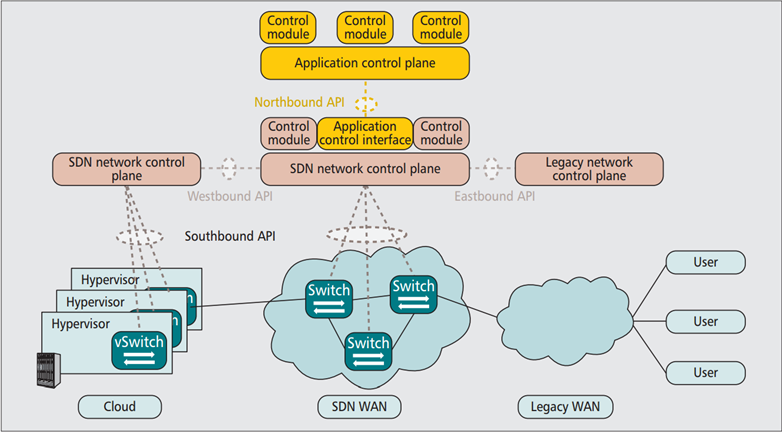
\includegraphics[width=13cm]{figure/ONF.png}
	\caption{The high-level SDN architecture.}
	\label{fig:{ONF}}
\end{figure}
\begin{itemize}
\item[] \textbf{Data Plane} : The data plane, or infrastructure plane, is the lowest layer in SDN architecture. This plane is composed by physical switches and virtual switches and others forwarding devices. Virtual switches are software-based switches, which can run on common operating systems. Open vSwitch \cite{OVS}, Indigo \cite{Indigo} and Pantou \cite{Pantou} are three implementations of virtual switches. Physical switches are hardware-based switches. They can be implemented on open network hardware (e.g., NetFPGA \cite{Lockwood2007}) or implemented on networking hardware vendors’ merchant switches. Many networking hardware vendors such as HP, NEC, Huawei, Juniper and Cisco, have supported SDN protocols. Virtual switches support complete features of SDN protocols, while physical switches lack the flexibility and feature completeness. However, physical switches have a higher flow forwarding rate than virtual switches.  SwitchBlade \cite{Anwer2010} and ServerSwitch \cite{Lu2011} are two NetFPGA-based physical switches.
These switches in data plane are responsible for forwarding, dropping and modifying packets based on instructions received from the Control Plane (CP) through Southbound Interfaces (SBIs).
\item[] \textbf{Control Plane}: The control plane is the “brain” of SDN systems, which can define network resources, dynamically choose forwarding rules and make network administration flexible and agile. The controller is responsable of many relevant tasks like:
\begin{itemize}
\item[•] the communication between forwarding devices and applications;
\item[•] it exposes and abstracts network state information of the data plane to the application plane;
\item[•] it translates the requirements from applications into custom policies and distributes them to forwarding devices;
\item[•] provides essential functionalities that most of network applications need, such as shortest path routing, network topology storage, device configuration and state information notifications etc.
\end{itemize}
There are many controller architectures, such as Ryu \cite{RYU}, OpenDayLight, \cite{Medved2014} NOX \cite{NOX}, POX \cite{POX}, Floodlight \cite{Floodlight} and Beacon \cite{Erickson2013}. Three communication interfaces allow the controllers to interact: southbound, northbound (NBI) and eastbound/westbound interfaces.
The	SBIs are defined between the control plane and the data plane. They allow forwarding devices to exchange network state information and control policies with the CP and provide functions such as statistics reports, forwarding operations, programmatic control of all device-capability advertisements and event notifications. OpenFlow \cite{McKeown2008} promoted by ONF is the first and the most popular open standard SBI. There exist other less popular proposals such as OVSDB \cite{OVS_Pfaff}, Protocol-Oblivious Forwarding (POF) \cite{Song2013} and OpenState \cite{Bianchi2014}. With NBIs, automation, innovation and management of SDN networks has been facilitate thanks to the fact that applications can exploit the abstract network views provided by the CP. The ONF is trying to define the standard NBIs and a common information model.
The eastbound/westbound interfaces are used in the multi-controller SDN networks. Due to the vast amount of data flows in such networks and the limited processing capacity of one controller the large-scale networks are always partitioned into several domains and each domain has its own controller.
The eastbound/westbound interfaces are responsible for the communication among multiple controllers. This communication  is necessary to exchange information in order to provide a global network view to the upper-layer applications. Onix \cite{Koponen} and HyperFlow \cite{Tootoonchian} are two distributed control architectures. Because their eastbound/westbound interfaces are private, they cannot communicate with each other. To enable the communication between different types of SDN controllers, SDNi \cite{yin2012}, East-West Bridge \cite{Lin2013} and Communication Interface for Distributed Control plane (CIDC) \cite{Benamrane2017} have been proposed as eastbound/westbound interfaces to exchange network information. However, the eastbound/westbound interfaces have not yet been standardized.
\item []\textbf{Application Plane}: The highest layer in the SDN architecture is the application plane. These applications can provide new services and perform business management, optimization and can obtain the required network state information through controllers’ NBIs. Based on the received information and other requirements, the applications can apply some control logic to change network behaviors.
The SDN-based applications have attracted a lot of attention from academia. Mendiola et al. \cite{Mendiola2017} have discussed the impact of SDN on Traffic Engineering (TE) and surveyed the SDN-based TE solutions. Security in SDN has been surveyed in \cite{Ahmad2015, ScottHayward2016, Rawat2017, Ali2015, Yan2016, Dargahi2017}. Especially, Yan et al. \cite{Yan2016} have researched on Distributed Denial of Service (DDoS) attacks in SDN-based cloud computing systems, and discussed future research challenges. Fault management in SDN has been surveyed in \cite{Fonseca2017}, which gives an identification and classification of the main fault management issues, and does valuable surveys and discussions about efforts that address those issues. Guck et al. \cite{Guck2018} have studied the centralized QoS routing mechanisms in SDN, and introduced a novel Four-Dimensional (4D) evaluation framework.
SDN has been deployed in many networks, such as transport networks \cite{Alvizu2017}, optical networks \cite{Thyagaturu2016}, wireless networks \cite{Haque2016, Chen2015}, Internet of Things (IoT) \cite{Bera2017}, edge computing \cite{Baktir2017}, Wide Area Networks (WAN) \cite{Michel2017}, cloud computing \cite{Jain2013}, Network Function Virtualization (NFV) \cite{Li2015, Liang2015}.
\end{itemize}
For more informations on SDN, please refer to \cite{Nunes2014, Jarraya2014, Xia2015, Hu2014, Xie2015, Trois2016, Huang2017, Blenk2016}.


\subsection{Workflow}
To understand the SDN architecture, it is important to recall its basic operation. Figure \ref{fig:{WorkFlow}} shows the working procedure of the OpenFlow-based SDN network \cite{OFP13}. Each OpenFlow switch has a flow table and uses the OpenFlow protocol to communicate with the SDN controller. The messages transmitted between the OpenFlow-based switches and the software-based controller are standardized by the OpenFlow protocol \cite{Erickson2013}. The OpenFlow controller can manage the traffic forwarding by modifying flow entries in switches flow tables.
\begin{figure}[tb!]
	\centering
	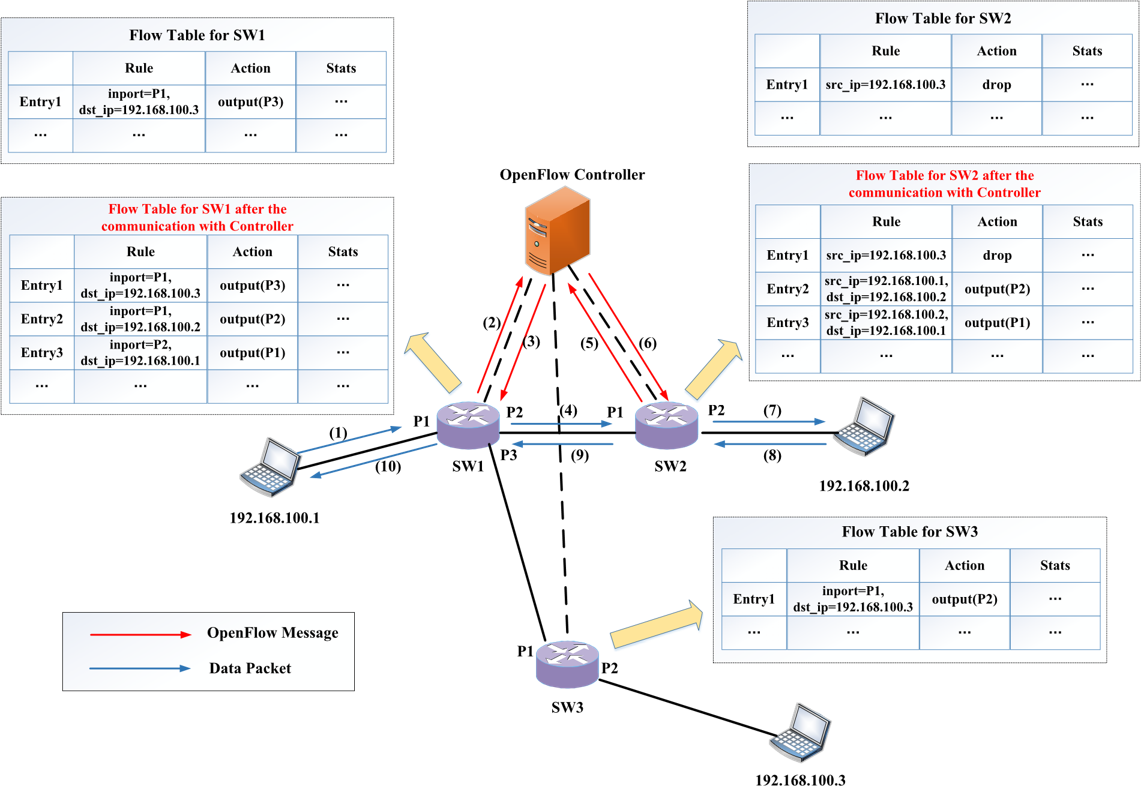
\includegraphics[width=13cm]{figure/WorkFlow.png}
	\caption{Example of OpenFlow-based SDN network.}
	\label{fig:{WorkFlow}}
\end{figure}
The flow table in the OpenFlow switch is comprised of flow entries to determine the processing actions of different packets on the data plane. When an OpenFlow switch receives a packet on the data plane, the packet header fields will be extracted and matched against flow entries. If a matching entry is found, the switch will process the packet locally according to the actions in matched flow entry. Otherwise, the switch will forward an OpenFlow PacketIn message to the controller (arrows 2 and 5). The packet header (or the whole packet, optionally) is included in the OpenFlow PacketIn message. Then, the controller will send OpenFlow FlowMod messages to manage the switch’s flow table by adding flow entries (arrows 3 and 6), which can be used to process subsequent packets of the flow.  For example, by adding two flow entries (i.e., Entry2 and Entry3) at SW1 and SW2, the communications between $192.168.100.1$ and $192.168.100.2$ are allowed.
However, packets from $192.168.100.3$ to $192.168.100.2$ are denied at SW2 due to security policies.
%====================================================================================================
%====================================================================================================
\section{Overview Of Machine Learning Algorithms} \label{sec:ML_BGK}
Machine learning is evolved from a collection of powerful techniques in AI areas. These methods start from training data to learn useful structural patterns and models. A machine learning approach consists of two main phases: the training phase and the decision making phase. In the training phase, after a data mining period that creates a training dataset, machine learning methods are applied to learn a system model. In the decision making phase, the trained model is used to estimate the output corresponding to each new input.
Machine learning algorithms can be distinguished into four main categories: supervised, unsupervised, semi-supervised and reinforcement learning.
\begin{figure}[tb!]
	\centering
	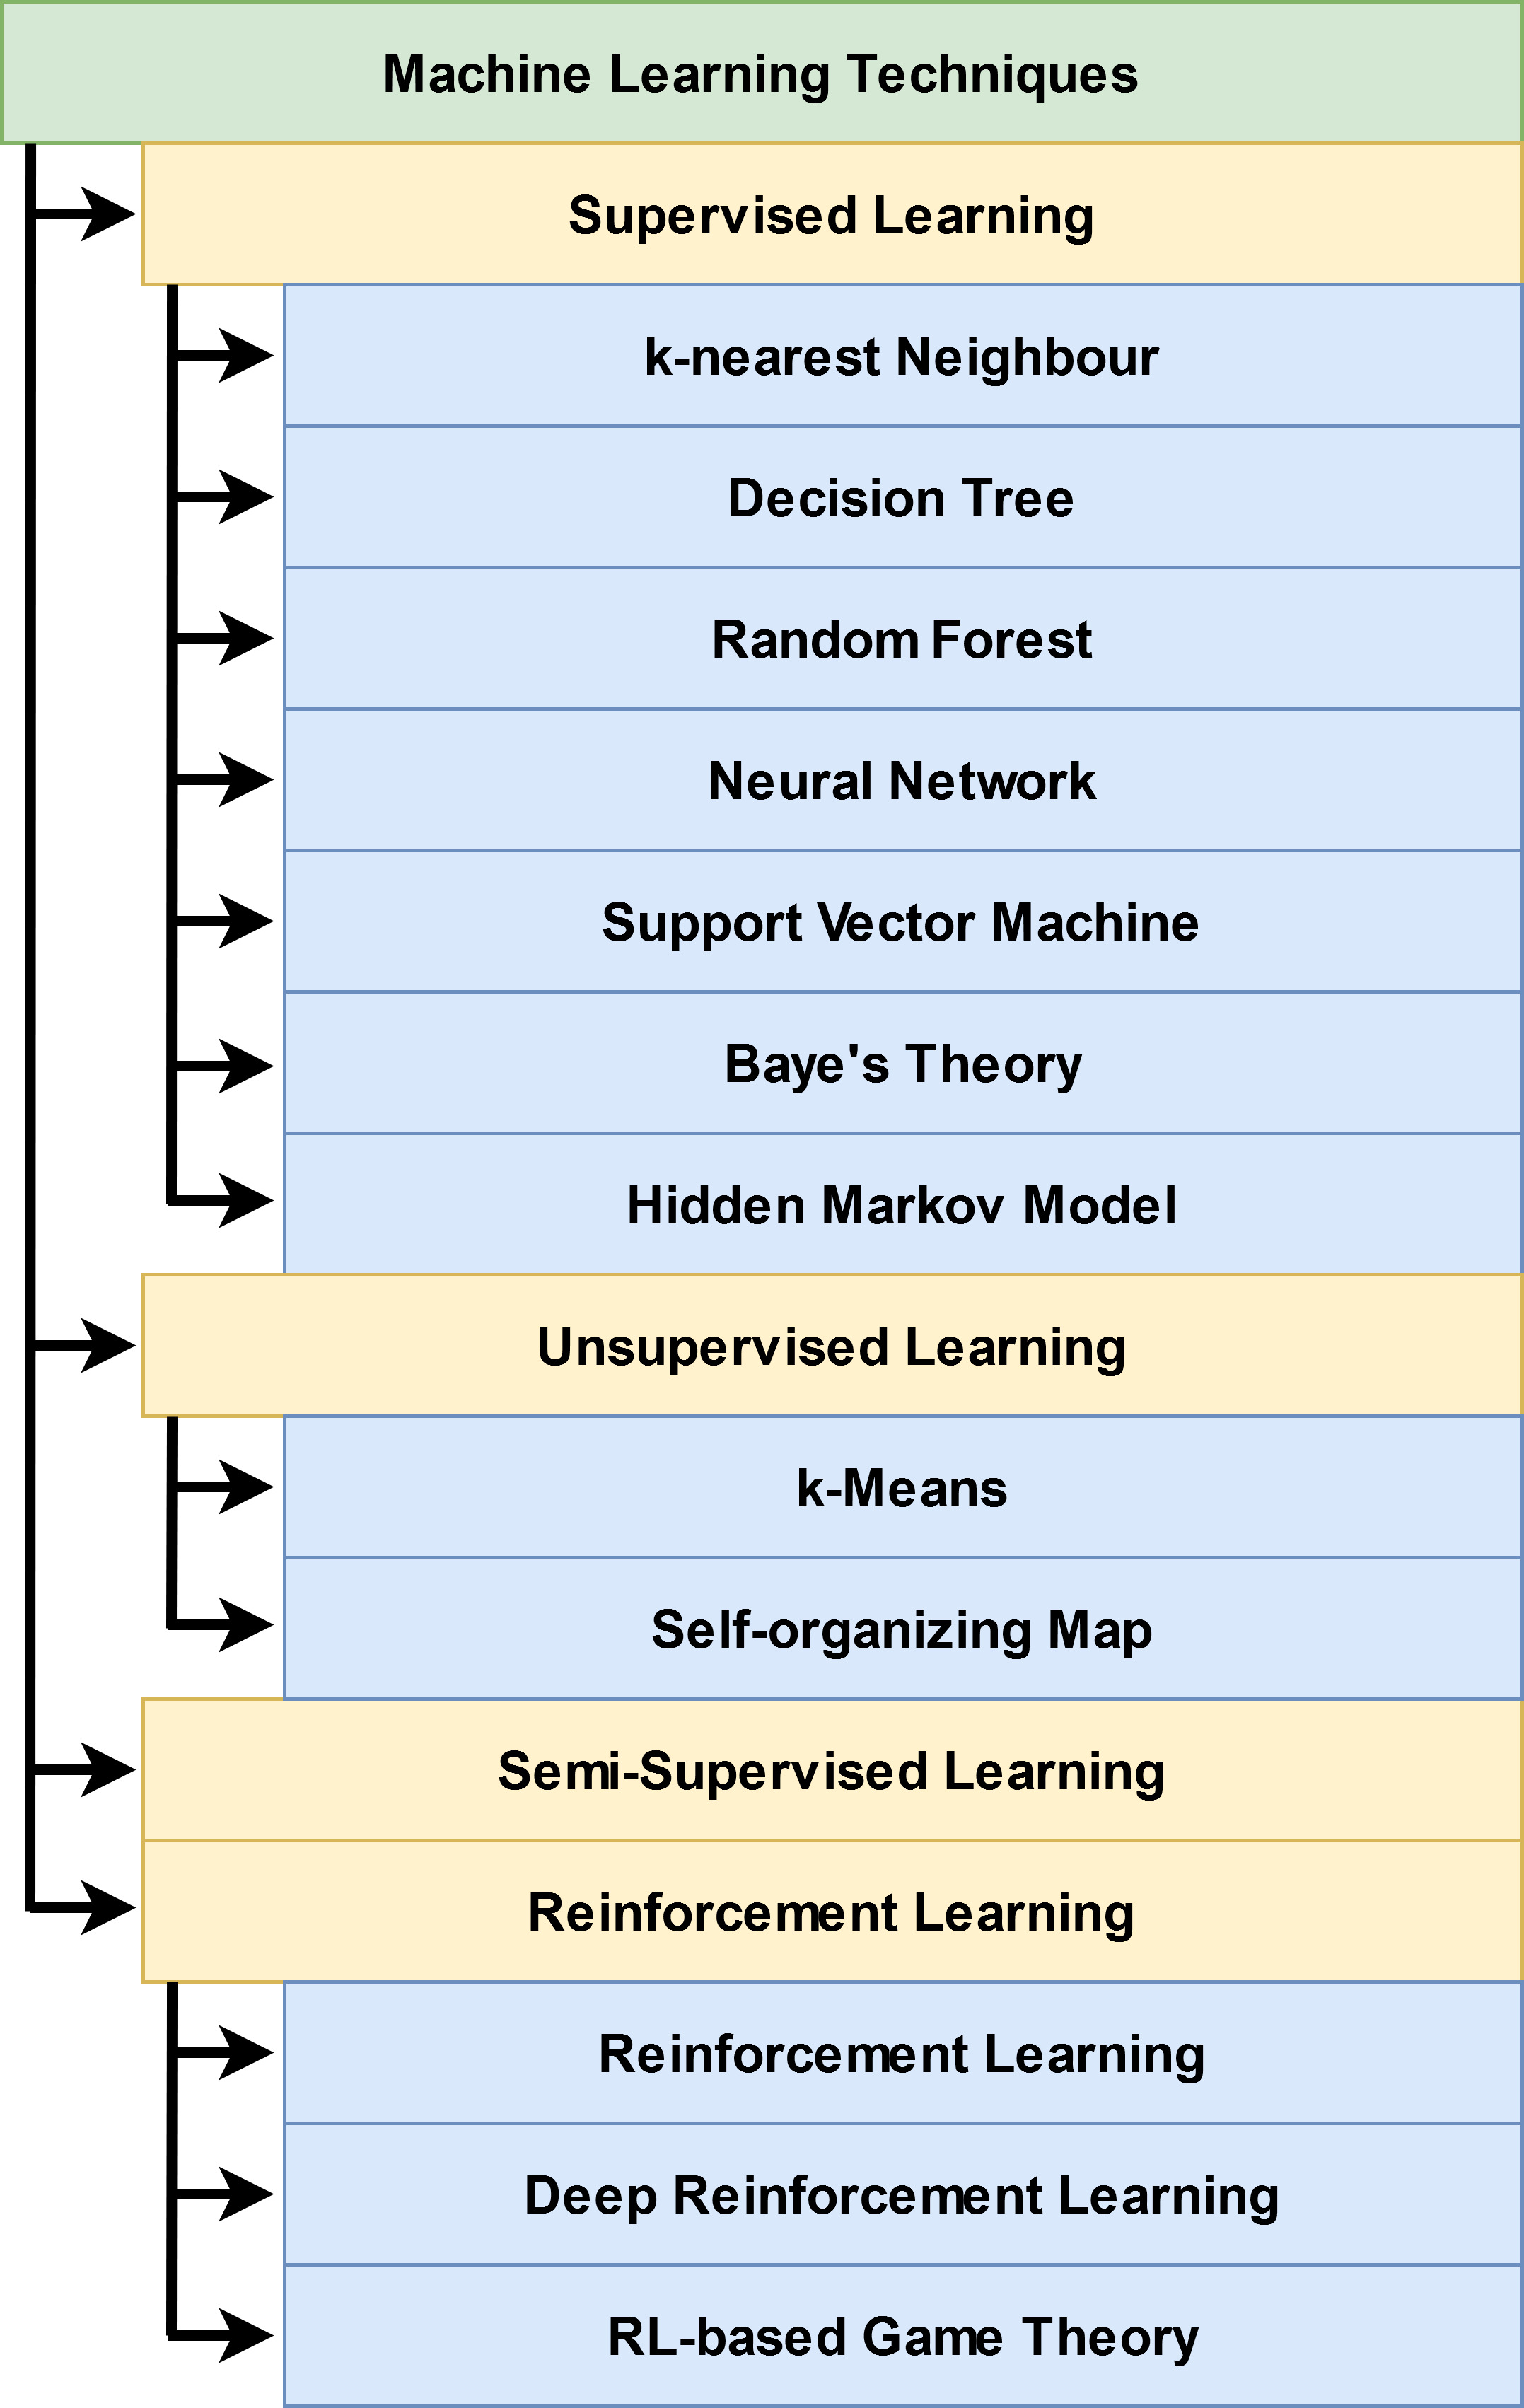
\includegraphics[scale=0.13]{figure/ML_algo.jpg}
	\caption{Common machine learning algorithms.}
	\label{fig:{ML_algo}}
\end{figure}
Each algorithm in Figure \ref{fig:{ML_algo}} is briefly explained with some examples. For a more insightful discussion on machine learning theory, please refer to \cite{Mohammed2016, Marsland2015, Alpaydin2020}.

\subsection{Supervised Learning}
Supervised learning is a kind of labelling learning technique. Supervised learning algorithms are given a labeled training dataset (i.e., inputs and known outputs) to build the system model representing the learned relation between the input and output. After training, when a new input is fed into the system, the trained model can be used to get the expected output \cite{Kotsiantis2007, Hastie2009}. In the following, an exhaustive representation of supervised learning algorithms is provided:
\begin{itemize}
\item[]\textit{1) k-Nearest Neighbor} (k-NN): In k-NN the classification of a data sample is determined based on the k nearest neighbors of that unclassified sample. The process of the k-NN algorithm is very simple: if the most of the k nearest neighbors belong to a certain class, the unclassified sample will be classified into that class. The higher the value of k is, the less effect the noise will have on the classification. Since the distance is the main metric of the k-NN algorithm, several functions can be applied to define the distance between the unlabeled sample and its neighbors, such as Chebyshev, City-block, Euclidean and Euclidean squared \cite{Cover1967}.
\item[]\textit{2) Regresstion Tree}: The RT performs classification through a learning tree. In the tree, each node represents a data feature, all branches represent the conjunctions of features that lead to classifications, and each leaf node is a class label. The unlabeled sample can be classified by comparing its feature values with the nodes of the RT \cite{Han2011}. The RT has many advantages, such as intuitive knowledge expression, simple implementation and high classification accuracy. ID3 \cite{Quinlan1986}, C4.5 \cite{Karatsiolis2012} and CART \cite{Burrows1995} are three widely-used decision tree algorithms. The biggest difference among them is the splitting criteria which are used to build decision trees. 
\item[]\textit{3) Random Forest}: A RF \cite{Breiman1999} consists of many RT. To mitigate over-fitting of RT methods and improve accuracy, the random forest method construct each RT by randomly choosing a subset of the features space . The steps to classify a new data sample by using random forest methods are:
\begin{itemize}
\item[]a) Put the data sample in each tree in the forest;
\item[](b) Each tree gives a classification result (vote);
\item[](c) The data sample will be classified into the class which has more votes.
\end{itemize}
\item[]\textit{4) Neural Network} (NN): A neural network is a computing system composed by a large number of simple processing units, which operate in parallel to learn experiential knowledge from historical data \cite{Haykin}. Each neuron performs highly complex, nonlinear and parallel computations. In a NN, its nodes are the equivalent components of the neurons in the human brain. These nodes use activation functions to perform nonlinear computations. The most frequently used activation functions are the sigmoid and the hyperbolic tangent functions. Simulating the way neurons are connected in the human brain, the nodes in a NN are connected to each other by variable link weights.
A NN has many layers. The first layer is the input layer, the last layer is the output layer and layers between them are the hidden layers. The output of each layer is the input of the next layer and the output of the last layer is the result. By changing the number of hidden layers and the number of nodes in each layer, complex models can be trained to improve the performance of NNs. NNs are widely used in many applications, such as pattern recognition. In figure \ref{fig:{NN_base}} the most basic NN with three layers has been shown. An input has $m$ features (i.e., $X_{1},X_{2},...,X_{m}$) and the input can be assigned to n possible classes (i.e., $Y_{1},Y_{2},...,Y_{n}$). Also, $W_{ij}^{1}$ denotes the variable link weight between the $ith$ neuron of layer $l$ and the $jth$ neuron of layer $l + 1$, and $ak^{l}$ denotes the activation function of the $kth$ neuron in layer $l$.
\begin{figure}[tb!]
	\centering
	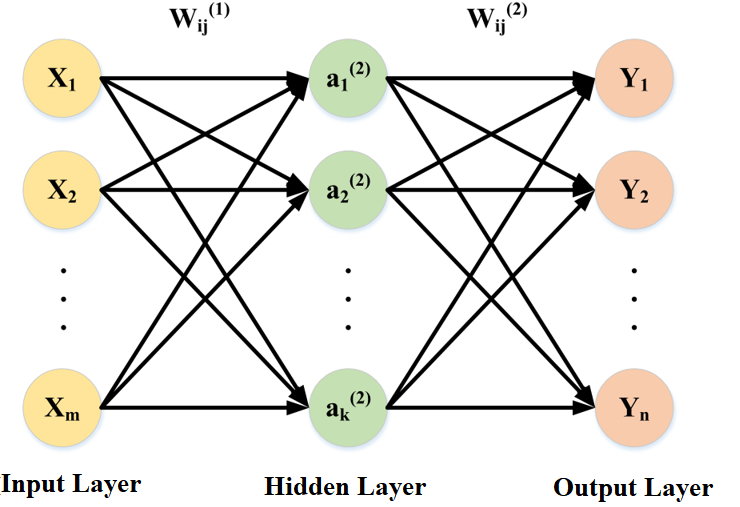
\includegraphics[width=13cm]{figure/NN_base.png}
	\caption{A basic neural network with three layers: an input layer, a hidden layer and an output layer.}
	\label{fig:{NN_base}}
\end{figure}
There are many types of neural networks, which can be divided in supervised or unsupervised main group \cite{Lee2005}. In the following, we will give a brief description of supervised neural networks.
\begin{itemize}
\item[]\textit{a)	Random NN}: The random NN can be represented as an interconnected network of neurons that exchange spiking signals. The main difference between random NN and other neural networks is that neurons in random NN exchange spiking signals probabilistically. In random NN, the internal excitatory state of each neuron is represented by an integer called “potential”. The potential value of each neuron rises when it receives an excitatory spiking signal and drops when it receives an inhibitory spiking signal. Neurons whose potential values are strictly positive are allowed to send out excitatory or inhibitory spiking signals to other neurons according to specific neurondependent spiking rates. When a neuron sends out a spiking signal, its potential value drops one. The random NN has been used in classification and pattern recognition \cite{Timotheou2010}.
\item[]\textit{b)	Deep NN}: Neural networks with a single hidden layer are generally referred to as shallow NNs. In contrast, neural networks with multiple hidden layers between the input layer and the output layer are called deep NNs \cite{LeCun2015, Schmidhuber2015}. To process high-dimensional data and to learn increasingly complex models, deep NNs with more hidden layers and neurons are needed. However, deep NNs increase the training difficulties and require more computing resources. In recent years, the development of hardware data processing capabilities and the evolved activation functions make it possible to train deep NNs \cite{Pandey2014}. In deep NNs, each layer’s neurons train a feature representation based on the previous layer’s output, which is known as feature hierarchy. The feature hierarchy makes deep NNs capable of handling large high-dimensional datasets. Due to the multiple-level feature representation learning, compared to other machine learning techniques, deep NNs generally provide much better performance \cite{Pandey2014}.
\item[]\textit{c)	Convolutional NN}: Convolutional NN and recurrent NN are two major types of deep NNs. Convolutional NN \cite{Krizhevsky2012, Li2018} is a feed-forward neural network. Local sparse connections among successive layers, weight sharing and pooling are three basic ideas of convolutional NN. Weight sharing means that weight parameters of all neurons in the same convolution kernel are same. Local sparse connections and weight sharing can reduce the number of training parameters. Pooling can be used to reduce the feature size while maintaining the invariance of features. The three basic ideas reduce the training difficulties of convolutional NNs greatly.
\item[]\textit{d)	Recurrent NN}: In feed-forward neural networks, the information is transmitted directionally from the input layer to the output layer. However, recurrent NN is a stateful network, which can use internal state (memory) to handle sequential data. Unlike a traditional deep NN, which uses different parameters at each layer, the recurrent NN shares the same parameters across all time steps. This means that at each time step, the recurrent NN performs the same task, just with different inputs. In this way, the total number of parameters needed to be trained is reduced greatly. Long Short-Term Memory (LSTM) \cite{Li2015a} is the most commonly-used type of recurrent NNs, which has a good ability to capture long-term dependencies. LSTM uses three gates (i.e., an input gate, an output gate and a forget gate) to compute the hidden state.
\end{itemize}
\item[]\textit{5) Support Vector Machine} (SVM): SVM is invented by Vapnik and others \cite{Vapnik1999}, which has been widely used in classification and pattern recognition. The basic idea of SVM is to map the input vectors into a high-dimensional feature space. This mapping is achieved by applying different kernel functions, such as linear, polynomial and Radial Based Function (RBF). Kernel function selection is an important task in SVM, which has effect on the classification accuracy. The selection of kernel function depends on the training dataset. The linear kernel function works well if the dataset is linearly separable. If the dataset is not linearly separable, polynomial and RBF are two commonly-used kernel functions. In general, the RBF-based SVM classifier has a relatively better performance than the other two kernel functions.
The objective of SVM is to find a separating hyperplane in the feature space to maximize the margin between different classes. The margin is the distance between the hyperplane and the closest data points of each class. The corresponding closest data points are defined as support vectors.
\item[]\textit{6) Bayes’ Theory}: Bayes’ theory uses the conditional probability to calculate the probability of an event occurring given the prior knowledge of conditions that might be related to the event. The Bayes’ theory is defined mathematically as the following equation:
\begin{equation*}
P(H\vert E)=\dfrac{P(E\vert H)P(H)}{P(E)}
\end{equation*}
where $E$ is a new evidence, $H$ is a hypothesis, $P(H\vert E)$ is the posterior probability that the hypothesis $H$ holds given the new evidence $E$, $P(E\vert H)$ is the posterior probability that of evidence $E$ conditioned on the hypothesis $H$, $P(H)$ is the prior probability of hypothesis $H$, independent of evidence $E$, and $P(E)$ is the probability of evidence $E$.
In a classification problem, the Bayes’ theory learns a probability model by using the training dataset. The evidence $E$ is a data sample, and the hypothesis $H$ is the class to assign for the data sample. The posterior probability $P(H\vert E)$ represents the probability of a data sample belonging to a class. In order to calculate the posterior probability $P(H\vert E)$, $P(H)$, $P(E)$ and $P(E\vert H)$ need to be calculated first based on the training dataset using the probability and statistics theories, which is the learning process of the probability model. When classifying a new input data sample, the probability model can be used to calculate multiple posterior probabilities for different classes. The data sample will be classified into the class with the highest posterior probability $P(H\vert E)$. The advantage of Bayes’ theory is that it requires a relatively small number of training samples dataset to learn the probability model \cite{Box2011}. However, there is an important independence assumption when using the Bayes’ theory. To facilitate the calculation of $P(E\vert H)$, the features of data samples in the training dataset are assumed to be independent of each other \cite{Bakker2017}.
\item[]\textit{7) Hidden Markov Models} (HMM): HMM is one kind of Markov models. Markov models are widely used in randomly dynamic environments which obey the 
memoryless property. The memoryless property of Markov models means that the conditional probability distribution of future states only relates to the value of the current state and is independent of all previous states \cite{Rabiner1989, Holgado2020}. There are other Markov models, such as Markov Chains (MC). The main difference between HMM and other models is that HMM is often applied in environments where system states are partially visible or not visible at all.
\end{itemize}
\subsection{Unsupervised Learning}
In contrast to supervised learning, an unsupervised learning algorithm is given a set of inputs without labels, thus there is no output. An unsupervised learning algorithm aims to find patterns, structures, or knowledge in unlabeled data by clustering sample data into different groups according to the similarity between them. The unsupervised learning techniques are widely used in clustering and data aggregation. In the following, we will give a representation of widely-used unsupervised learning algorithms.
\begin{itemize}
\item[]\textit{1)	k-Means}: The k-means algorithm is used to recognize a set of unlabeled data into different clusters. To implement the kmeans algorithm, only two parameters are needed: the initial dataset and the desired number of clusters. If the desired number of clusters is k, the steps to resolve node clustering problem by using k-means algorithms are:
\begin{itemize}
\item[]\textit{a)} initialize k cluster centroids by randomly choosing k nodes;
\item[]\textit{b)} use a distance function to label each node with the closest centroid;
\item[]\textit{c)} assign new centroids according to the current node memberships;
\item[]\textit{d)} stop the algorithm if the convergence condition is valid, otherwise go back to step \textit{b)}.
\end{itemize}
\item[]\textit{2)	Self-Organizing Map} (SOM): SOM, also known as SelfOrganizing Feature Map (SOFM) \cite{Kohonen2012}, is one of the most popular unsupervised neural network models. SOM is often applied to perform dimensionality reduction and data clustering. In general, SOM has two layers, an input layer and a map layer. When SOM is used to perform data clustering, the number of neurons in the map layer is equal to the desired number of clusters. Each neuron has a weight vector. The steps to resolve data clustering problem by using SOM algorithm are:
\begin{itemize}
\item[]a) initialize the weight vector of each neuron in the map layer;
\item[](b) choose a data sample from the training dataset;
\item[](c) use a distance function to calculate the similarity between the input data sample and all weight vectors. The neuron whose weight vector has the highest similarity is called the Best Matching Unit (BMU). The SOM algorithm is based on competitive learning;
\item[](d) The neighborhood of the BMU is calculated;
\item[](e) The weight vectors of the neurons in the BMU’s neighborhood are adjusted towards the input data sample;
\item[](f) Stop the algorithm if the convergence condition is valid, otherwise go back to step (b).
\end{itemize}
\end{itemize}
\subsection{Semi-Supervised Learning}
Semi-supervised learning is a type of learning which uses both labeled and unlabeled data. Semi-supervised learning is useful due the fact that in many real-world applications, the acquisition of labeled data is expensive and difficults while acquiring a large amount of unlabeled data is relatively easy and cheap. Moreover effective use of unlabeled data during the training process actually tends to improve the performance of the trained model. In order to make the best use of unlabeled data, assumptions have to be hold in semisupervised learning, such as smoothness assumption, cluster assumption, low-density separation assumption, and manifold assumption. Pseudo Labeling \cite{Wu2018} is a simple and efficient semi-supervised learning technique. The main idea of Pseudo Labeling is simple. Firstly, use the labeled data to train a model. Then, use the trained model to predict pseudo labels of the unlabeled data. Finally, combine the labeled data and the newly pseudo-labeled data to train the model again. There are other semi-supervised learning methods, such as Expectation Maximization (EM), co-training, transductive SVM and graph-based methods. Different methods rely on different assumptions. For example, EM builds on cluster assumption, transductive SVM builds on low-density separation assumption, while graph-based methods build on the manifold assumption.
\subsection{Reinforcement Learning}
Supervised learning algorithms are generally applied to conduct classification and regression tasks, while unsupervised and reinforcement learning algorithms are applied to conduct clustering and decision-making tasks respectively.
\begin{itemize}
\item[]\textit{1)	Reinforcement Learning} (RL): RL \cite{Sutton2018, Kaelbling1996} involves an agent, a state space S and an action space A. The agent is a learning entity which interacts with its environment to learn the best action to maximize its long-term reward. The long-term reward is a cumulative discounted reward and relates to both the immediate reward and future rewards. When applying RL to SDN, the controller generally works as an agent and the network is the environment. The controller monitors the network status and learns to make decisions to control data forwarding. Specifically, at each time step $t$, the agent monitors a state $s_{t}$ and chooses an action $a_{t}$ from the action space $A$, receives an immediate reward $r_{t}$ which indicates how good or bad the action is, and transitions to the next state $st+1$. The objective of the agent is to learn the optimal behavior policy $\pi$ which is a direct map from the state space S to the action space $A (\pi : S \longrightarrow A)$ to maximize the expected long-term reward. From the behavior policy $\pi$, the agent can determine the best corresponding action given a particular state. In RL, value function is used to calculate the long-term reward of an action given a state. The most well-known value function is Q-function, which is used by Q-learning to learn a table storing all state-action pairs and their long-term rewards.
\item[]\textit{2)	Deep Reinforcement Learning} (DRL): The main advantage of RL is that it works well without prior knowledge of an exact mathematical model of the environment. However, the traditional RL approach has some shortcomings, such as low convergence rate to the optimal behavior policy $\pi$ and its inability to solve problems with high-dimensional state space and action space. These shortcomings can be addressed by DRL. The key idea of DRL is to approximate the value function by leveraging the powerful function approximation property of deep NNs. After training the deep NNs, given a state-action pair as input, DRL is able to estimate the long-term reward. The estimation result can guide the agent to choose the best action.
\item[]\textit{3)	RL-Based Game Theory}: Game theory is a mathematical tool that focuses on strategic interactions among rational decision-makers. A game generally involves a set of players, a set of strategies and a set of utility functions. Players are decision-makers. Utility functions are used by players to select optimal strategies. In cooperative games, players cooperate and form multiple coalitions. Players choose strategies that maximize the utility of their coalitions. In non-cooperative games, players compete against each other and choose strategies individually to maximize their own utility. In the network field, it is often assumed that nodes are selfish.
In non-cooperative games, players do not communicate with each other, and at the beginning of each play round, players do not have any information about the strategies selected by the other players. At the end of each play round, all players broadcast their selected strategies, which are the only external information. However, each player’s utility can be affected by the other players’ strategies. In this case, adaptive learning methods should be used to predict the strategies of the other players, based on which each player chooses its optimal strategy. RL is a widely-used adaptive learning method, which can help players select their optimal strategies by learning from historical information such as network status, the other players’ strategies and the corresponding utility. Thus, RL-based game theory is an effective decision-making technique.
\end{itemize}

%====================================================================================================

\addcontentsline{toc}{chapter}{PART II: Problem Formulations}
\chapter*{\centering PART II: Problem Formulations}  

\chapter{Network emulation environment} \label{sec:SDNNetSim}
The Mininet environment \cite{Mininet} has been used to emulate a SDN network to validate the methodology that will be presented in terms of prediction accuracy and control performance. This software runs a collection of virtual network elements (i.e. end-hosts, switches, routers, and links) on a single Linux kernel using lightweight virtualization. 
%To test the effectiveness of the realized controller a simulated network has been programmed using the Mininet environment as a network emulation orchestration system. This software runs a collection of end-hosts, switches, routers, and links on a single Linux kernel by using lightweight virtualization to make a single system look like a complete network. Mininet's virtual objects emulate real SDN network devices. It is usually possible to create a Mininet network that resembles a hardware network, or a hardware network that resembles a Mininet network, and to run the same binary code and applications on either platform.
To generate traffic the D-ITG generator \cite{Avallone2004, Botta2012, Botta2013} has been used.

\begin{figure}[htb!]
	\centering
	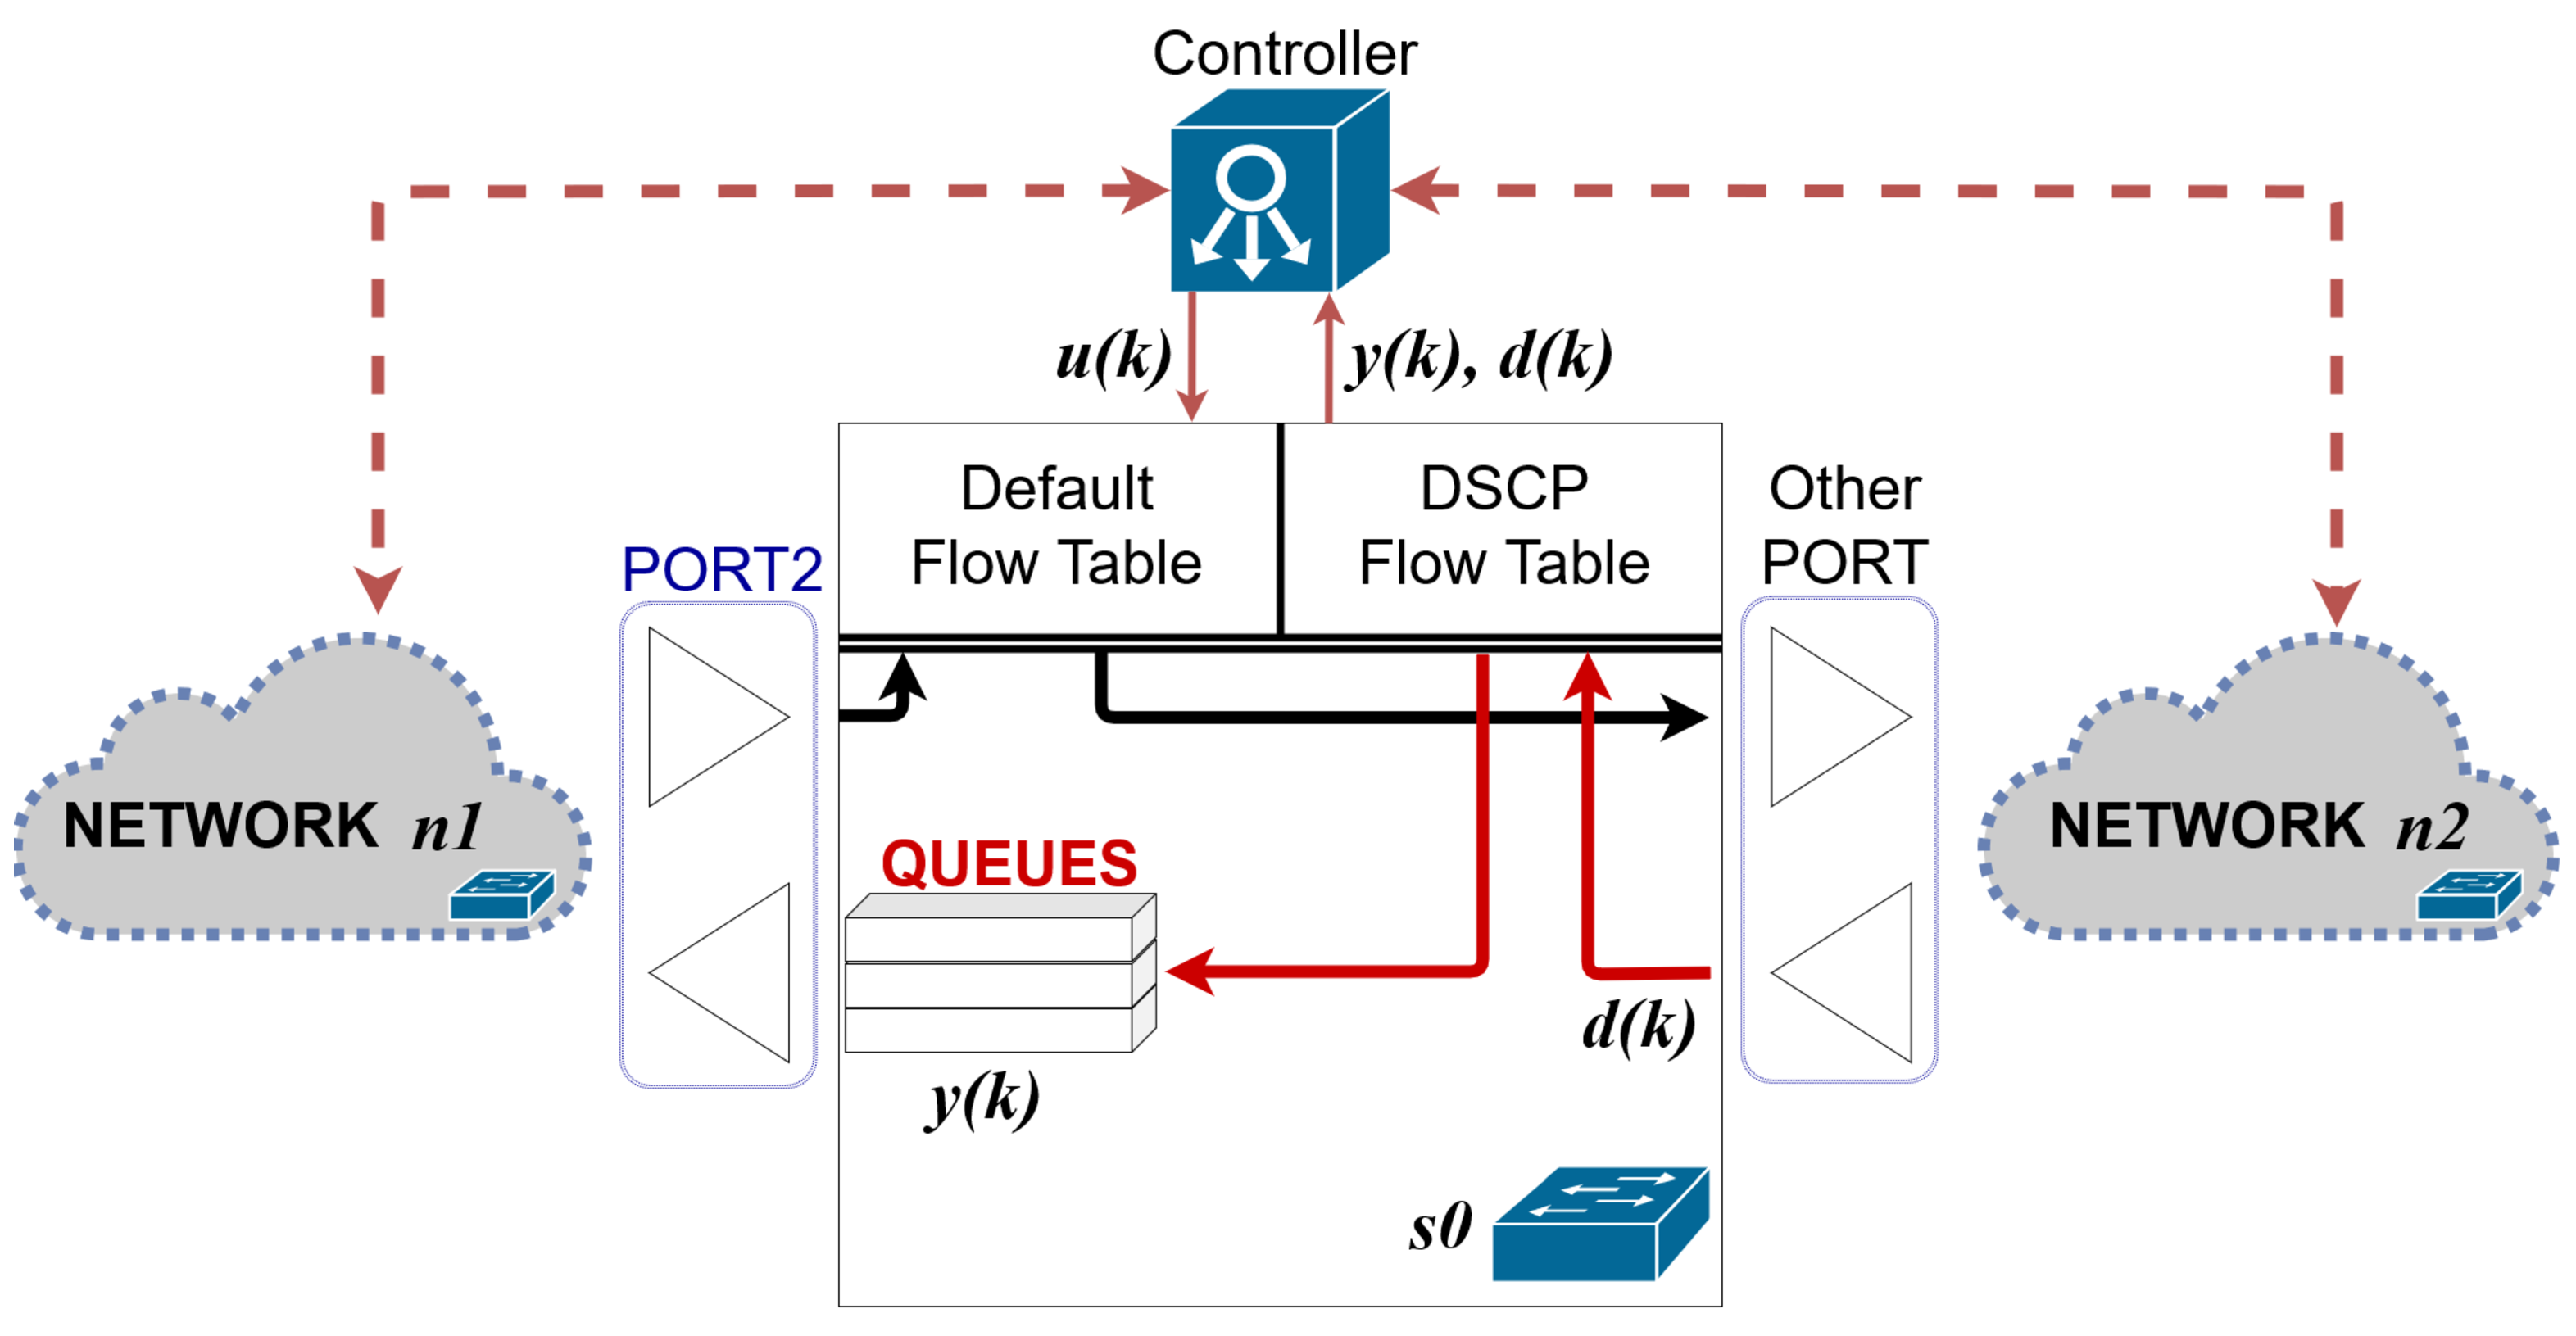
\includegraphics[keepaspectratio,width=\columnwidth]{figure/SDN_net_EPS.eps}
	\caption{Mininet emulated network architecture.}
	\label{fig:{Network}}
\end{figure}
%\begin{figure}[tb!]
%	\centering
%	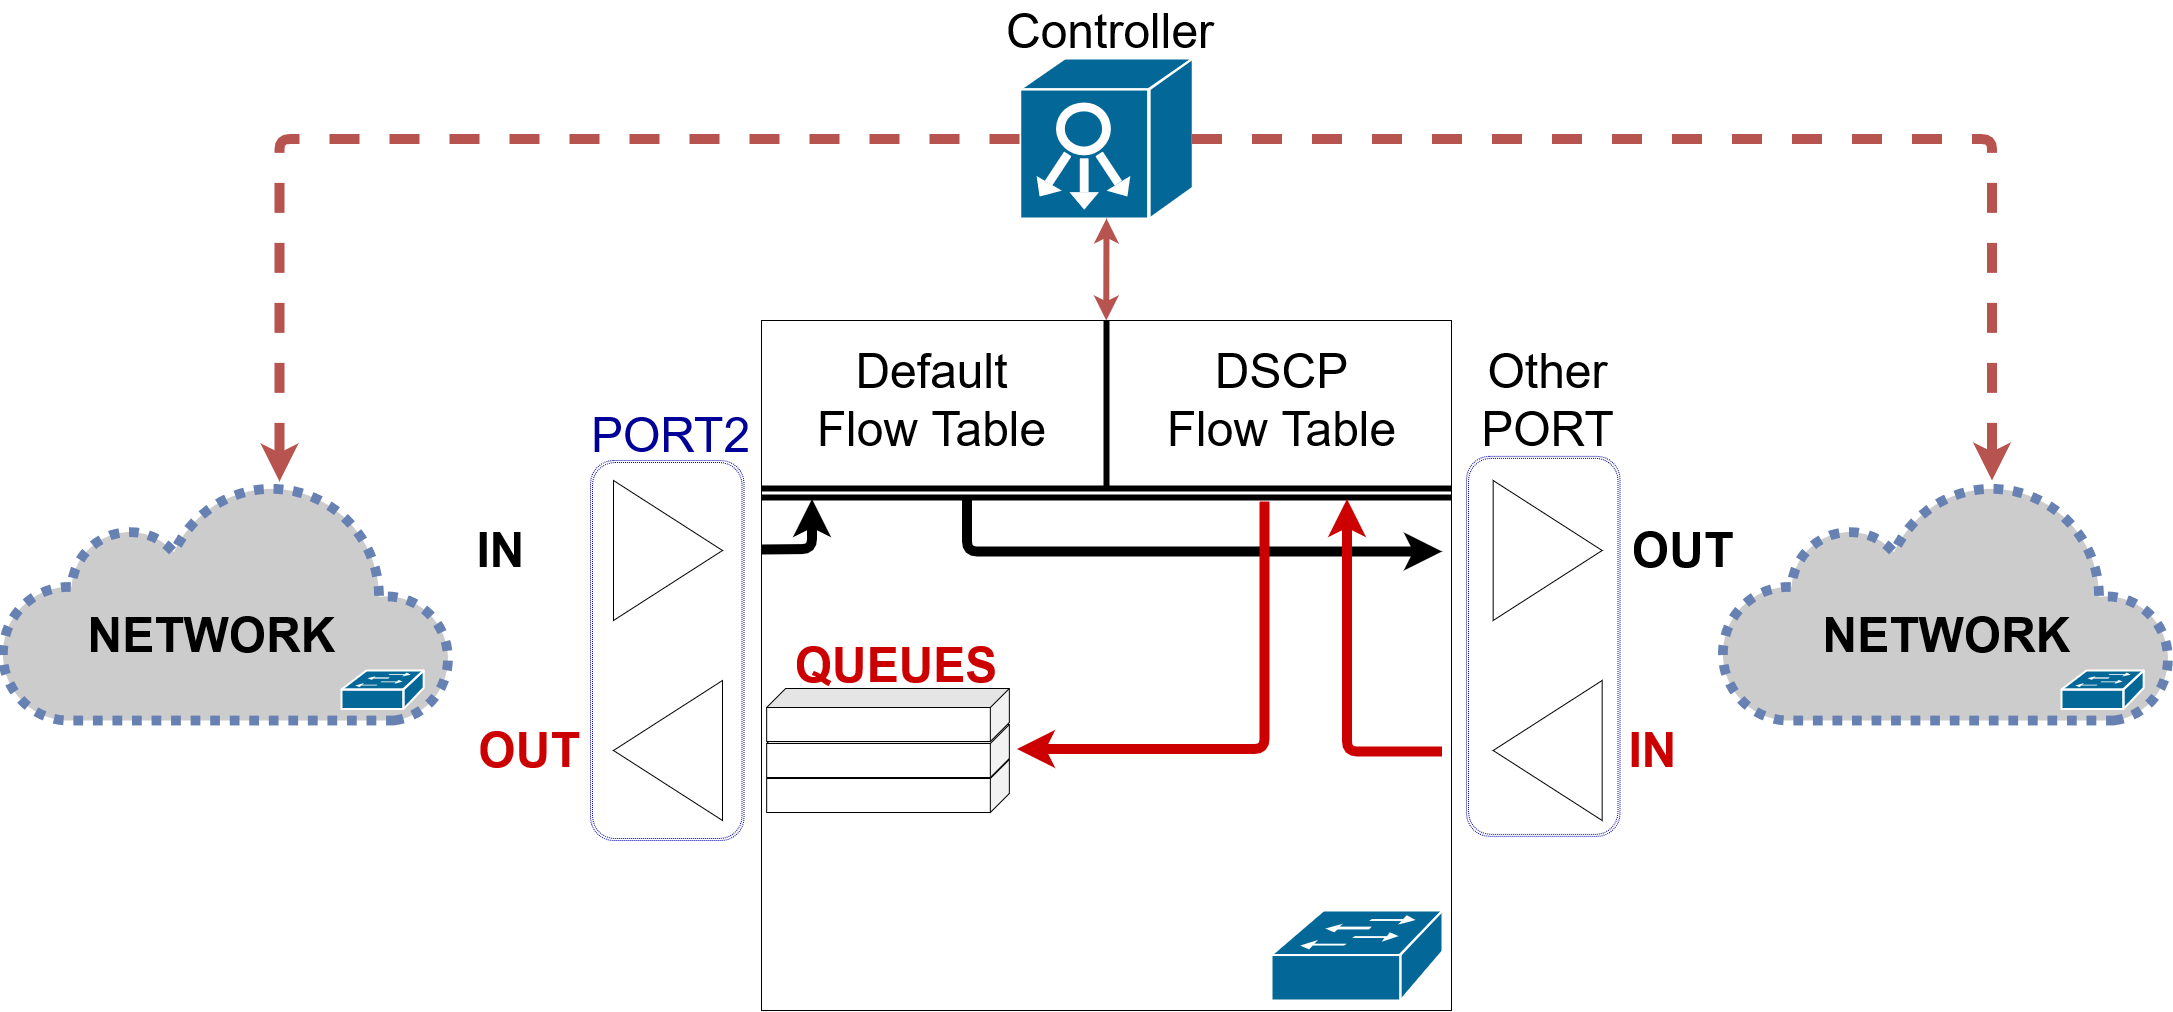
\includegraphics[width=13cm]{figure/SDN_net_LAST.png}
%	\caption{Simulated Network inside Mininet environment.}
%	\label{fig:{Network}}
%\end{figure}

A network architecture as in Figure \ref{fig:{Network}} has been considered, which aims at representing a portion of a larger network where a bottleneck occurs. More precisely, a switch $s0$ with one input port and one output port, and a remote controller \cite{OVS, RYU} that dynamically manages the configuration of the queues of $s0$ has been emulated. The input of $s0$ is fed with more instance of D-ITG generating stochastic traffic, whose mean value follows the pattern of a real data set (where packets are differentiated by their ToS - Type of Service - priority index) extracted from two days logs of a router of a large service provider network. Namely, the original real data set contains traffic of a real network incoming from a source geographic area and terminating in a destination geographic area, and is divided for each value of Differentiated Services Code Point (DSCP) with a sampling time of 5 minutes \cite{Baker1998, Babiarz2006}. DSCP is the modern definition of the Type of Service (ToS) field, in which the first 6 bits are the Differentiated Services field that are in common with ToS field, and the last 2 bits regard explicit congestion notification. The ToS field can specify the priority of a datagram and the request for a low delay addressing, a high throughput or a high reliability service. Following the implementation of many national service provider networks (see e.g. \cite{Notiziario}), the 8 different values of the DSCP has been partitioned in three classes: the \textit{Default} class (DSCPs $0,1,3$), the \textit{Premium} (DSCPs $2,4,6,7$), and the \textit{Gold} class (DSCP $5$): each queue has been assigned to a single queue, associated with a different priority.

%Traffic generation is entrusted to the D-ITG generator which uses informations inside a database created from a real measure that contains the number of packets transmitted and received by a switch. The database fields has been divided for each type of Differentiated Services Code Point (DSCP) with a sampling time of 5 minutes \cite{Baker1998, Babiarz2006}. DSCP is the modern definition of the Type of Service (ToS) field in which the first 6 bits are the Differentiated Services field that are in common with ToS field, and the last 2 bits are the explicit congestion notification. The ToS field can specify the priority of a datagram and the request for a low delay addressing, a high throughput or a high reliability service. Depending on the ToS values, a packet could be placed in a high priority exit queue, or follow a route with latency, throughput and the appropriate reliability for the request.


Using D-ITG Sender and Receiver SW modules it has been possible to establish a connection between networks n1 and n2. In particular, 16 ITG modules have been initialized: 8 for each network, and within each network one for each DSCP index. These modules handle the sampling time interval (5 minutes), the inter-departure time stochastic distribution associated with the packet rate, the packet size stochastic distribution, the IP and port destinations, and the DSCP index. Regarding the controller SW module RYU has been used, which provides software components with well defined Application Programming Interfaces (API) that give the possibility to easily create new network management and control applications. Ryu supports various protocols for managing network devices, such as OpenFlow, Netconf, OF-config, etc. About OpenFlow, Ryu supports fully 1.0, 1.2, 1.3, 1.4, 1.5 and Nicira Extensions. For the used test-bed the 1.3 version has been chosen. In particular, APIs were used for queue control and counter recovery from the switches \cite{ofctlrest,QoS}. The feedback information collected for the purposes of this work are the descriptions of switches, ports and queues, the number of packets received and transmitted on each port of a switch, the packets passing through the flow tables, the packet rate values of each queue and the packets transmitted by each single queue. In summary, the variables associated to the traffic and control signals in the closed-loop architecture are as follows:

\begin{itemize}
	\item $d(k)\in\Real^{10}$ is a measurable disturbance vector, i.e. representing variables that cannot be controlled. The first 8 components $d_1(k),\ldots,d_8(k)$ consist of the number of packets incoming in the switch $s0$ differentiated with respect to the 8 different values of the DSCPs. $d_9(k)$ and $d_{10}(k)$ are proxy variables, i.e. the hours and minutes of the day, which are very useful to the predictive model since traffic dynamics are tightly correlated with them, e.g. they are substantially different between night and day;
	\item $y(k)\in\Real^{3}$ is the measured output vector, i.e. the variables to regulate. They consist of the number of packets outgoing from switch $s0$ differentiated with respect to the corresponding service class: $y_1(k)$ is the Default Queue output, $y_2(k)$ is the Premium Queue output and $y_3(k)$ is the Gold Queue output;
	\item $u(k)\in\Real^{3}$ is the control input vector. Each component corresponds to the queue configuration of each service class: $u_1(k)$ is the Default Queue configuration, i.e. the maximum admitted bandwidth; $u_2(k)$ is the Premium Queue configuration, i.e. the maximum admitted bandwidth; $u_3(k)$ is the Gold Queue configuration, i.e. the minimum admitted bandwidth;
\end{itemize}

\begin{figure}[tb!]
	\centering
	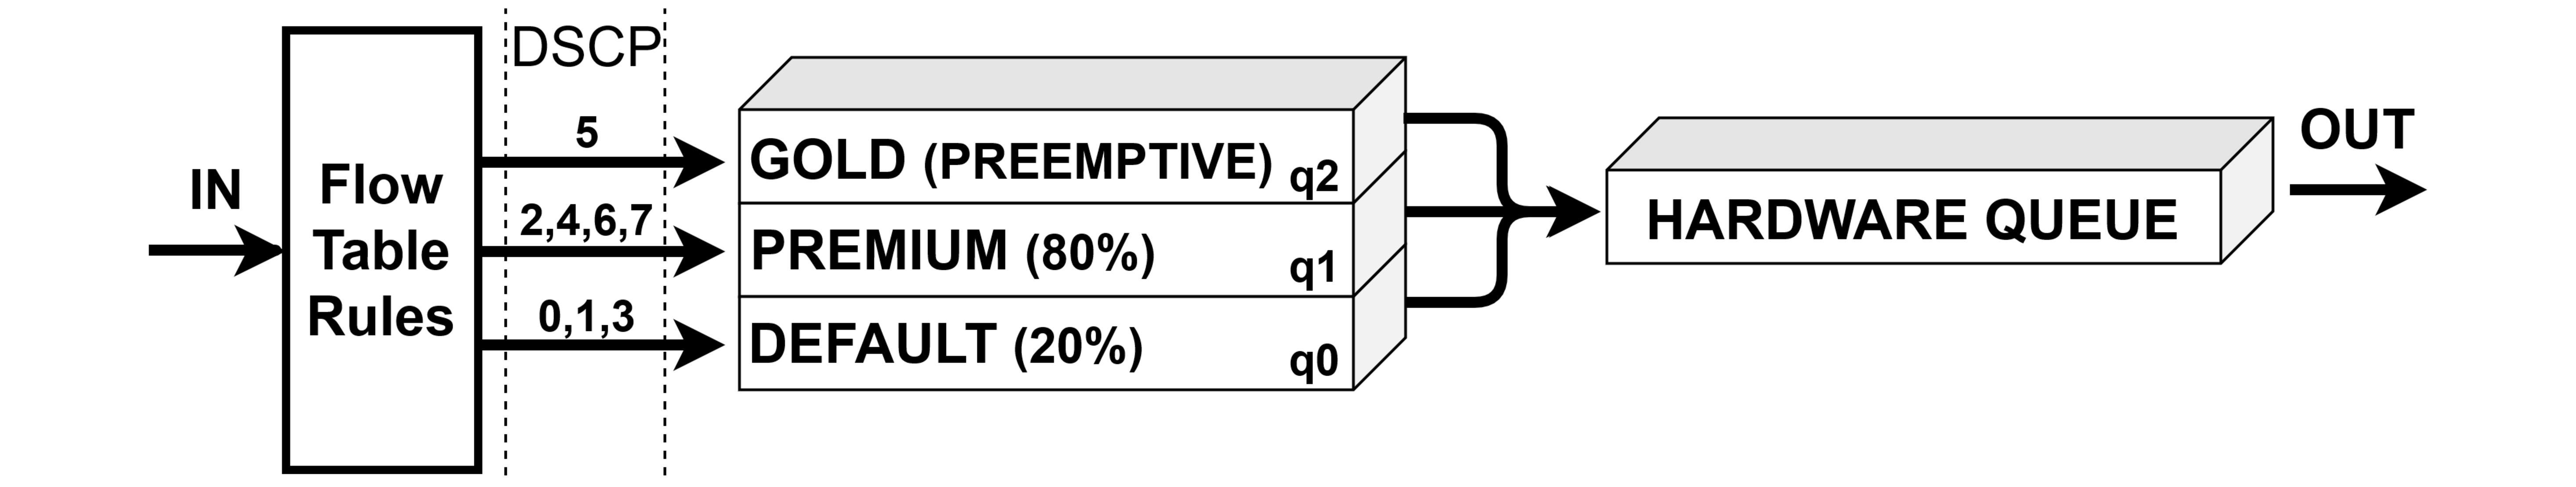
\includegraphics[keepaspectratio,width=\columnwidth]{figure/QUEUE.eps}
%	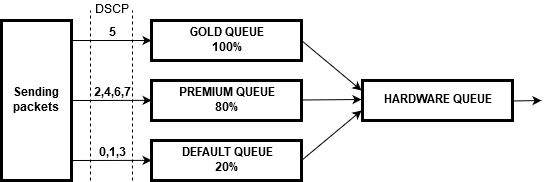
\includegraphics[keepaspectratio,width=12cm]{figure/queue.png}
	\caption{Static queues rate with routed packets relative to DSCP.}
	\label{fig:{queue}}
\end{figure}

In this work the static control of queues used in the Italian service provider network of \textit{Telecom Italia} \cite{Notiziario} has been first applied in the chosen emulative scenario, which is depicted in Figure \ref{fig:{queue}}. To this aim 3 queues in $s0$ and has been defined and configured as follows: packets with the DSCP values 0, 1 and 3 (Default queue) are routed via queue 0, with maximum rate $u_1(k) = 20 \textit{MB/s}, \forall k$; the packets with values 2, 4, 6 and 7 (Premium queue) are routed on queue 1, with maximum rate $u_2(k) = 80 \textit{MB/s}, \forall k$; the packets with value 5 (Gold queue) are routed on queue 2, with minimum rate $u_3(k) = 100 \textit{MB/s}, \forall k$. To obtain this prioritization it has also been necessary to set the flow tables of $s0$ to discriminate incoming packets based on the DSCP value and the destination IP address, and re-route them to the desired queue. Also, to obtain a bottleneck situation in $s0$, the bandwidth of the output port of switch $s0$ has been setted at 100 \textit{MB/s}. Using this configuration queue 2 uses the maximum capacity of the port to forward packets with preemptive priority, while the other two queues use the remaining bandwidth from 0 \textit{MB/s} to the specified maximum bandwidth based on needs.\\
%As formally defined later in Section \ref{secSwitchedModeling}, the packets sent by the queues will be collected in the state vector to be controlled $x(k)\in\mathbf{R}^3,\ \forall k$,  while the bandwidth associated to the queues will compose the control variables vector $u(k)\in\mathbf{R}^3,\ \forall k$.
As will be shown in Section \ref{secExpRes}, using static priority control the queues will not be able to send all the packets incoming from network $n1$, and a dramatic amount of packets will be lost. This motivates the application of optimization techniques, which are enabled by the predictive models derived using the methodology described in the following section.
%\textcolor{blue}{In this work we first applied in our emulative scenario the static control of queues used in the Italian service provider network of \textit{Telecom Italia} \cite{Notiziario}, which is depicted in Figure \ref{fig:{queue}}. To this aim we defined 3 queues in $s0$ and configured the queues as follows: packets with the DSCP values 0, 1 and 3 (Default queue) are routed via queue 0, with maximum rate $u_1(k) = 20 \textit{MB/s}, \forall k$; the packets with values 2, 4, 6 and 7 (Premium queue) are routed on queue 1, with maximum rate $u_2(k) = 80 \textit{MB/s}, \forall k$; the packets with value 5 (Gold queue) are routed on queue 2, with minimum rate $u_3(k) = 100 \textit{MB/s}, \forall k$. To obtain this prioritization it has also been necessary to set the flow tables of $s0$ to discriminate incoming packets based on the DSCP value and the destination IP address, and re-route them to the desired queue. Also, to obtain a bottleneck situation in $s0$, we have chosen the bandwidth of the output port of switch $s0$ at 100 \textit{MB/s}. Using this configuration queue 2 uses the maximum capacity of the port to forward packets with preemptive priority, while the other two queues use the remaining bandwidth from 0 \textit{MB/s} to the specified maximum bandwidth based on needs.\\
%As we will see in Section \ref{secExpRes}, using static priority control the queues will not be able to send all the packets incoming from network $n1$, and a dramatic amount of packets will be lost. This motivates the application of optimization techniques, which are enabled by the predictive models derived using the methodology described in the following section.}

%\begin{figure}[tb!]
%	\centering
%	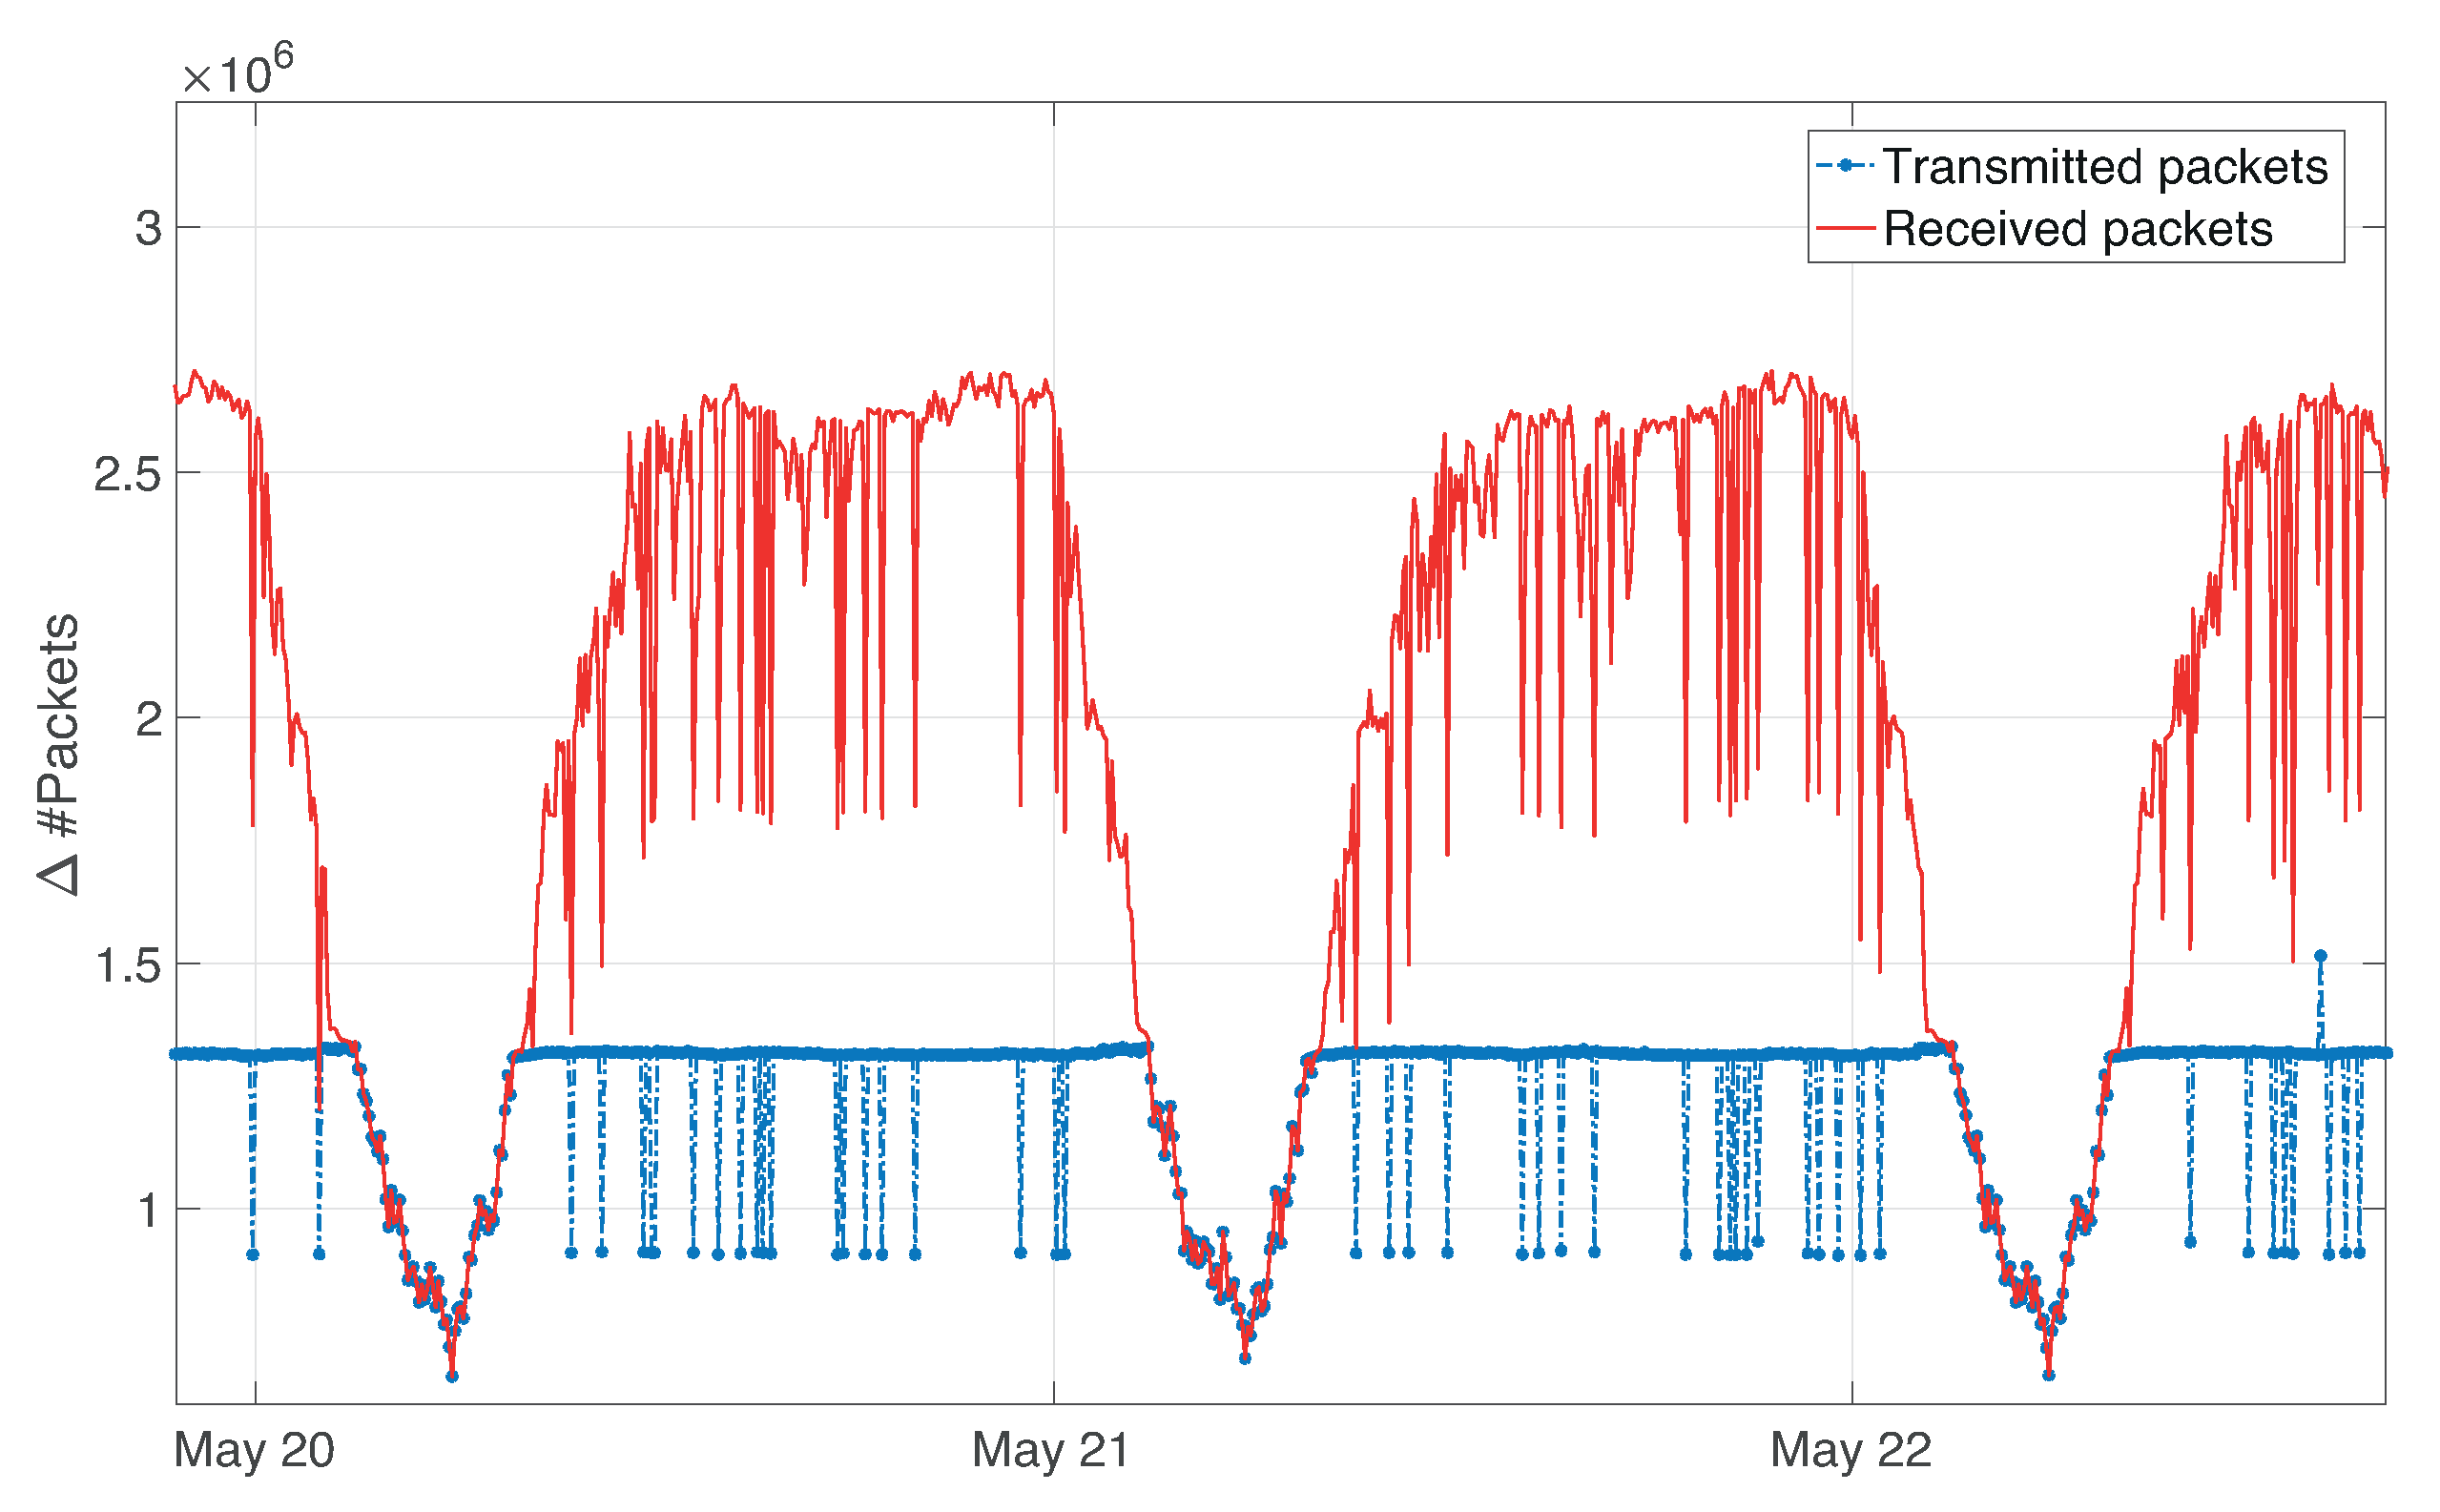
\includegraphics[keepaspectratio,width=\columnwidth]{figure/traffic2Cut.eps}
%	\caption{Received vs. transmitted packets in s0 using static priority as in \cite{Notiziario}.}
%	\label{fig:{Traffic}}
%\end{figure}
%Simulation plots in Figure \ref{fig:{Traffic}} clearly show that using static priority control, as expected, the queues are not able to send all the packets incoming from network n1, and a dramatic amount of packets is lost. This motivates the application of optimisation techniques, which are enabled by the predictive models derived using the methodology described in the following section.


%====================================================================================================
%====================================================================================================
%\newpage
\section{Switched affine modeling via RT and RF}\label{secSwitchedModeling}
%====================================================================================================

\textbf{\emph{Problem formulation.}} In this section it is illustrated the methodology to apply the results proposed in \cite{SmarraADHS2018,smarraNAHS2020} to identify, starting from a set of collected historical data $ \mathcal{D}=\{y(k),u(k),d(k)\}_{k = 0}^{\ell} $ as illustrated in the previous section, a switching ARX model of input-output behavior of the traffic flow in a switch of a SDN network as follows:
%The aim of such predictive model is to enable the direct and computationally efficient implementation of Model Predictive Control for bandwidth and packet losses optimisation.
\small
\begin{equation}\label{eqIdentifiedModelNSARX}
x(k+j+1) =	A'_{\sigma_j(x(k),d(k))} x(k) + \sum_{\alpha = 0}^{j}B'_{\sigma_{j}(x(k),d(k)),\alpha} u(k+\alpha) + f'_{\sigma_j(x(k),d(k))},
\end{equation}
\normalsize
\noindent $j = 0,\ldots, N-1$, where $x(k) \doteq [y^\top(k)\ \cdots\ y^\top(k-\delta_y)\ u^\top(k-1)\ \cdots\ u^\top(k-\delta_u)]^\top\in\Real^{n_x}$ is an extended state to characterize a switching ARX model, with $x_\iota(k) \doteq [y_\iota(k)\ \cdots\ y_\iota(k-\delta_y)\ u^\top(k-1)\ \cdots\ u^\top(k-\delta_u)]^\top\in\Real^{\delta_y+1+3\delta_u}$, $\iota = 1,2,3$, $N$ is the chosen future predictive horizon, and  $\sigma_j : \mathbb{R}^{n_x+10} \to \mathcal M \subset \mathbb{N}$ is a switching signal that associates an operating mode in a finite set $\mathcal M$ to each pair $(x(k),d(k))$ and each prediction step $j$ of the horizon.
It is possible to directly use model \eqref{eqIdentifiedModelNSARX} to setup the following problem, which can be solved using standard Quadratic Programming (QP) solvers:\\
\begin{problem}\label{pbMPCSwitching}
	\small
	\vspace{-0.3cm}
	\begin{equation*}
		\begin{aligned}
			& \underset{u_0,\ldots,u_{N-1}}{\text{minimize}} & &  \sum_{j=0}^{N-1} \left(\left(x_{j+1}-x_{\mathrm{ref}}\right)^\top Q \left(x_{j+1}-x_{\mathrm{ref}}\right) + u^\top_{j} R u_{j}\right)\\
			& \text{subject to }            & &  x_{j+1} = A'_{\sigma_j(x_{0},d_{0})} x_0 + \sum_{\alpha = 0}^{j}B'_{\sigma_{j}(x_{0},d_{0}),\alpha} u_\alpha + f'_{\sigma_j(x_{0},d_{0})}\\       
			&                               & &  u_{j}   \in \mathcal{U}\\
			&                               & &  x_{0} = x(k), d_{0} = d(k)\\ 
			&                               & &  j = 0,\ldots,N-1.			\\
		\end{aligned}
		\vspace{0.1cm}
	\end{equation*}
	\normalsize
\end{problem}
\noindent As it is well known \cite{borrelli2017predictive}, Problem \ref{pbMPCSwitching} is solved at each time step $k$ using QP to compute the optimal sequence $u^*_0,\ldots,u^*_{N-1}$, but only the first input is applied to the system, i.e. $u(k) = u^*_0$. Note that, for any prediction step $j$, $x_{j+1}$ only depends on the measurements $x_0=x(k),d_0=d(k)$ at time $k$, since they are the only available measurements at time-step $k$. 
%\subsection{Switching ARX Identification using RF}\label{secSARX}

%====================================================================================================

\textbf{\emph{RT and RF background.}} Let us consider a dataset $\{y(k),x_1(k),\ldots,x_\eta(k)\}_{k=0}^\ell$, with $y,x_1,\ldots,x_\eta\in\mathbb{R}$. Let us suppose  to estimate, using Regression Trees, the prediction of the (response) variable $y(k)$ using the values of predictor variables $x_1(k),\ldots,x_\eta(k)$. The CART algorithm \cite{BreimanCART2017} creates a RT structure via optimal partition of the dataset. It solves a Least Square problem by optimally choosing recursively a variable to split and a corresponding splitting point. After several steps the algorithm converges to the optimal solution, and the dataset is partitioned in hyper-rectangular regions (the leaves of the tree) $R_1, R_2,\cdots, R_\nu$. In each partition $y(k)$ is estimated with a different constant $\hat y_i\, i=1,\ldots,\nu,$ given by the average of the samples of $y(k)$ falling in $R_i$, i.e.

\begin{equation}\label{eqAverageResponseRT}
\hat y_{i} = \frac{\sum\limits_{\{k|(x_1(k),\ldots, x_\eta(k)) \in R_i\}}y(k)}{|R_i|}
\end{equation}


\noindent Random Forests \cite{BreimanML2001} are instead an averaging method that exploits a combination of tree predictors such that each tree depends on the values of a random vector sampled independently and with the same distribution for all trees in the forest. The output prediction is given by averaging the predictions provided by all trees in the forest. It is possible to show that the error introduced by the forests quickly and almost surely converges to a limit as the number of trees in the forest becomes large. Such error also depends on the strength of the individual trees in the forest and the correlation between them. Thus, due to the Law of Large Numbers, Random Forests (differently from Regression Trees) do not suffer much variance and overfitting problems. For more details the reader is refered to \cite{BreimanCART2017,BreimanML2001}.

%====================================================================================================

\textbf{\emph{Switching ARX (SARX) model identification via RT.}} To derive a model as in \eqref{eqIdentifiedModelNSARX}, a new dataset $\X= \{x(k),u(k),d(k)\}_{k = 0}^{\ell}$ has to be defined starting from $\D$. In order to apply MPC it is needed, for each component of $y(k)$, a model that can predict system's dynamics over a horizon of length $N$. The idea is to create $3 N$ predictive trees $\{\mathcal{T}_{\iota,j}\},\ \iota=1,2,3,\ j=0,\ldots,N-1$, each one to predict the 3 outputs components of the system over the $N$ steps of the horizon. To create the tree structure, the RT algorithm (CART) partitions the dataset $\X$ into regions $\X_i$, such that $\biguplus \X_i = \X$, and assigns to each region a constant value given by the average of the output values of the samples that ended up in that leaf. In run-time, once the trees are created, and given a real-time measurement $(x(k), u(k), d(k))$ belonging to leaf $i$, the CART algorithm provides as a prediction the averaged value associated to the leaf as in \eqref{eqAverageResponseRT}. However, since the prediction provided by the RT is a constant value, it cannot be used to setup an MPC problem, thus the learning procedure needs to be modified to identify a modeling framework as in \eqref{eqIdentifiedModelN}. To this end, $\X$ is partitioned in two disjoint sets $\mathcal{X}_c = \{u(k)\}_{k=0}^{\ell}$ of data associated to the control variables, and $\mathcal{X}_{nc} = \{(x(k), d(k))\}_{k=0}^{\ell}$ of data associated to remaining variables, and then apply the CART algorithm only on $\mathcal{X}_{nc}$ (this is to avoid that the MPC problem turns out into a Mixed Integer Quadratic Program, see \cite{SmarraADHS2018,smarraNAHS2020} for details); thus, $3 N$ RTs $\{\mathcal{T}_{\iota,j}\}$ have been created, each constructed to predict the variable $y_\iota(k+j+1)$, and consequently $x_\iota(k+j+1)$. In particular, it is associated to each leaf $\iota,i_j$, corresponding to the partition  $\mathcal{X}_{nc,\iota,i_j}$, of each tree $\mathcal{T}_{\iota,j}$ the following affine model

\small

\begin{equation}\label{eqLTIleavesSinglState}
	x_\iota(k+j+1) = A'_{\iota,i_j}x(k) + \sum_{\alpha = 0}^{j}{B'_{\iota,i_j,\alpha}u(k+\alpha)} + f'_{\iota,i_j},
\end{equation}
\normalsize
\small
\begin{equation}\label{eqLeafModel}
\begin{aligned}
A'_{\iota,i_j} =& \left[\begin{array}{cccccccccc}
a_1       & a_2       & \cdots & a_{\delta_y } & a_{\delta_y + 1} & b_{\delta_y + 2} & \cdots & b_{\delta_y + 1+ 3(\delta_u-1)} & \cdots & b_{\delta_y + 1 + 3\delta_u} \\
1         & 0         & \cdots & 0             & 0                & 0                & \cdots & 0                               & \cdots & 0                            \\
\vdots    & \vdots    & \ddots & \vdots        & \vdots           & 0                & \cdots & 0                               & \cdots & 0                            \\
0         & 0         & \cdots & 1             & 0                & 0                & \cdots & 0                               & \cdots & 0                            \\
0         & 0         & \cdots & 0             & 0                & 0                & \cdots & 0                               & \cdots & 0                            \\
0         & 0         & \cdots & 0             & 0                & 0                & \cdots & 0                               & \cdots & 0                            \\
0         & 0         & \cdots & 0             & 0                & 0                & \cdots & 0                               & \cdots & 0                            \\
0         & 0         & \cdots & 0             & 0                & 1                & \cdots & 0                               & \cdots & 0                            \\
\vdots    & \vdots    & \ddots & \vdots        & \vdots           & \vdots           & \ddots & \vdots                          & \ddots & \vdots                       \\
0         & 0         & \cdots & 0             & 0                & 0                & \cdots & 1                               & \cdots & 0                            \\

\end{array}\right],\\
B'_{\iota,i_j,\alpha} = & \left[\begin{array}{ccc}
b_{1,\alpha} & b_{2,\alpha} & b_{3,\alpha}\\
0            & 0            & 0            \\
\vdots       & \vdots       & \vdots \\
0            & 0            & 0            \\   
0            & 0            & 0            \\  
0            & 0            & 0            \\  
0            & 0            & 0            \\  
0            & 0            & 0            \\  
\vdots       & \vdots       & \vdots            \\   
0            & 0            & 0            \\   
\end{array}\right],\ \alpha<j,\ 
B'_{\iota,i_j,j} =  \left[\begin{array}{ccc}
b_{1,\alpha} & b_{2,\alpha} & b_{3,\alpha}\\
0            & 0            & 0            \\
\vdots       & \vdots       & \vdots \\
0            & 0            & 0            \\   
1            & 0            & 0            \\  
0            & 1            & 0            \\  
0            & 0            & 1            \\  
0            & 0            & 0            \\  
\vdots       & \vdots       & \vdots            \\   
0            & 0            & 0            \\   
\end{array}\right],\ 
f'_{\iota,i_j} = \left[\begin{array}{ccccc}
f      \\	0 \\ \vdots \\ 0 \\ 0 \\ 0 \\ 0 \\ 0 \\ \vdots \\ 0      
\end{array}\right],
\end{aligned}
\end{equation}
\normalsize

\noindent where the coefficients of matrices $A'_{\iota,i_j}$, $B'_{\iota,i_j,\alpha}$ and $f'_{\iota,i_j}$ are obtained in each leaf $\iota,i_j$ by fitting the corresponding set of samples solving the following Least Squares with inequality constraints problem:

\begin{problem}\label{pbLeastSquareProblem}
	\small
	\begin{alignat}{2}
		& \nonumber \underset{\xi_{\iota,i_j}}{\text{minimize}} & &  \parallel \Lambda_{\iota,i_j} \xi_{\iota,i_j}  - \lambda_{\iota,i_j} \parallel_2^2   		 \\
		& \text{subject to }    \nonumber            & &  f_\mathrm{min} \leq f \leq f_\mathrm{max}    										  					 \\
		&                  					    	 & &  a_\mathrm{min} \leq a_{\jmath} \leq a_\mathrm{max}\label{eqInequalityConstraints} \\
		& 	                    \nonumber			 & &  b_\mathrm{min} \leq b_{\iota,\alpha} \leq b_\mathrm{max},
	\end{alignat}
	\normalsize
\end{problem}

\noindent where $\xi_{\iota,i_j}$, $\lambda_{\iota,i_j}$, and $\Lambda_{\iota,i_j}$ contain respectively the parameters of matrices in \eqref{eqLeafModel}, the predictions $x_\iota(k+j+1)$, and the current measurements of $x(k)$ and $u(k+\alpha)$. Linear inequalities \eqref{eqInequalityConstraints} are used to constrain elements in $\xi_{\iota,i_j}$ to take into account physical system constraints and improve prediction accuracy.
Model \eqref{eqLTIleavesSinglState} can be easily compacted in the following form taking into account all the states $\iota=1,2,3$:
\small
\begin{equation}\label{eqLTIleavesCompact}
x(k+j+1) = A'_{i_j}x(k) + \sum_{\alpha = 0}^{j}{B'_{i_j,\alpha}u(k+\alpha)} + f'_{i_j}.
\end{equation}
\normalsize
\noindent In particular, with the specific choice of $\delta_u = 0$ model \eqref{eqIdentifiedModelNSARX} can be rewritten in the following state-space formulation
\small
\begin{equation}\label{eqIdentifiedModelN}
x(k+j+1) =	A_{\sigma_j(x(k),\bold{u^-}(k),d(k))} x(k+j) + B_{\sigma_j(x(k),\bold{u^-}(k),d(k))} u(k+j) + f_{\sigma_j(x(k),\bold{u^-}(k),d(k))},
\end{equation}
\normalsize
where $\bold{u^-}(k) = [u^\top(k-1)\ \cdots\ u^\top(k-\delta)]^\top$ is the vector with the regressive terms of the input used to only grow the trees, and  $\sigma_j : \mathbb{R}^{3(\delta_y+1)+3\delta+10} \to \mathcal M \subset \mathbb{N}$.
%\noindent In particular, as anticipated in the problem formulation, with the specific choice of $\delta_u = 0$ matrices $A'_{\iota,i_j}$ in \eqref{eqLeafModel} modify as follows:
%
%\small
%\begin{equation}\label{eqLeafModelDelta_u=0}
%	\begin{aligned}
%		A'_{\iota,i_j} =& \left[\begin{array}{ccccc}
%			a_1       & a_2       & \cdots & a_{\delta_y } & a_{\delta_y + 1} \\
%			1         & 0         & \cdots & 0                         & 0     \\
%			\vdots    & \vdots    & \ddots & \vdots                    & \vdots     \\
%			0         & 0         & \cdots & 1                         & 0     
%		\end{array}\right]\\
%		B'_{\iota,i_j,\alpha} = & \left[\begin{array}{ccccc}
%			b_{1,\alpha} & 0 & \cdots & 0 & 0\\
%			b_{2,\alpha} & 0 & \cdots & 0 & 0           \\
%			b_{3,\alpha} & 0 & \cdots & 0 & 0           \\   
%		\end{array}\right]^\top\\
%				f'_{\iota,i_j} = &\left[\begin{array}{ccccc}
%		f      &	0 & \cdots & 0 & 0      
%		\end{array}\right]^\top.
%	\end{aligned}
%\end{equation}
%%\normalsize
Thanks to this new formulation the following proposition shows that model \eqref{eqLTIleavesCompact} is equivalent to model \eqref{eqIdentifiedModelN} for any initial condition, any switching signal and any control sequence.
\begin{proposition}\label{propSwitchingSystem}\cite{smarraNAHS2020}
	Let $A'_{i_j}$, $B'_{i_j,\alpha}$ and $f'_{i_j}$, $\alpha=0,\ldots,j$, $j=0,\ldots,N-1$, be given. If $A'_{i_j}$ is invertible for $j=0,\ldots,N-1$, then there exists a model in the form
	\vspace{-0.2cm}
	\small
	\begin{equation*}
	\bar x({k+j+1}) = A_{\sigma_j(\bar x(k),\bold{u^-}(k), d(k))} \bar x({k+j})+B_{\sigma_j(\bar x(k),\bold{u^-}(k), d(k))} u({k+j})+ f_{\sigma_j(\bar x(k),\bold{u^-}(k), d(k))}	
	\end{equation*}
	\normalsize
	such that for any initial condition $\bar x(k) = x(k) = x_k$, any switching sequence $i_0, \ldots, i_{N-1}$ and any control sequence $u(k),\ldots,u(k+N-1)$, then $\bar x(k+j+1) = x(k+j+1),\ \forall j=0,\ldots,N-1$.
\end{proposition}

As discussed in \cite{smarraNAHS2020}, from experimental findings it is possible to notice that the contribution in terms of model accuracy introduced by the choice of $\delta_u = 0$ is negligible, since previous control inputs are already considered in the tree structure choosing $\delta > 0$. Thus, in the rest of the paper it will be considered $\delta_u = 0$ and $\delta > 0$, i.e. only the regressive terms of the input in the tree structure learning will be used and not in the state definition.

\textbf{\emph{SARX model identification via RF.}} RF-based models can be constructed exploiting the RT-based formulation: in particular, let us consider $3 N$ RFs $\mathcal{F}_{\iota,j}$, $\iota = 1,2,3,\ j = 0,\ldots,N-1$. 
For each tree $\mathcal{T}^{\mathcal{F}_{\iota,j}}_\tau$ of the forest $\mathcal{F}_{\iota,j}$, it is possible to estimate the coefficients $a_*$, $b_*$ and $f$ in \eqref{eqLeafModel} for each leaf $\iota,j,i_\tau$, i.e. $\tilde\xi_{\iota,j,i_\tau}$, solving Problem \ref{pbLeastSquareProblem}.
With a small abuse of notation, let us indicate by $|\mathcal{F}_{\iota,j}|$ the number of trees in the forest ${\iota,j}$. 
Then $\forall \iota,j$, the parameters to build matrices in \eqref{eqLTIleaves} can be obtained by averaging parameters $a_*$, $b_*$ and $f$, $\forall \tau = 1,\ldots,|\mathcal{F}_{\iota,j}|$, i.e.
\small
\begin{equation}\label{eqAverageRF}
\tilde\xi_{\iota,j} = \frac{\sum\limits_{\tau=1}^{|\F_{\iota,j}|}\tilde\xi_{\iota,j,i_\tau}}{|\F_{\iota,j}|},
\end{equation}
\normalsize
over all the trees of forest $\F_{\iota,j}$. At this point, starting from \eqref{eqLTIleavesSinglState}, it can be easily construct the following model, as in \eqref{eqLTIleavesCompact} to be used in the MPC formulation by combining for $\iota=1,2,3$ the matrices in \eqref{eqLeafModel} coming either from the RTs or from the RFs:
\small
\begin{equation}\label{eqLTIleaves}
	x(k+j+1) = A'_{i_j}x(k) + \sum_{\alpha = 0}^{j}{B'_{i_j,\alpha}u(k+\alpha)} + f'_{i_j}.
\end{equation}
\normalsize

%====================================================================================================

\textbf{\emph{MPC problem formulation.}} It is used model \eqref{eqLTIleaves} to formalize Problem \ref{pbMPCSwitching} according to the SDN priority queueing problem:
\begin{problem}\label{pbMPC}

	\begin{equation*}
		\begin{aligned}
			& \underset{\bold u}
			{\text{minimize}}               & &  \sum_{j=0}^{N-1} \Big[(x_{j+1}-x_{\mathrm{ref},j})^\top Q (x_{j+1}-x_{\mathrm{ref},j}) + u^\top_{j} R u_{j}\Big]   \\
			& \text{subject to}             & &  x_{j+1}  =   A_{\sigma_j(k)} x_{j}+B_{\sigma_j(k)}  u_j+f_{\sigma_j(k)} \\
			&								& &  \Delta u_\iota^\mathrm{min} \leq u_{\iota,j} - u_{\iota,j-1} \leq \Delta u_\iota^\mathrm{max}             \\
			&								& &  u_\iota^\mathrm{min} \leq u_{\iota,j} \leq u_\iota^\mathrm{max}             \\
			&                               & &  u_{1,j} + u_{2,j} \leq 100			          		\\
			&                               & &  x_0 = x(k),\ \bold u^-_{0} = [u^\top(-1)\ \cdots\ u^\top(-\delta)]^\top,\ d_0 = d(k),\\
			&								& &  j = 0,\ldots,N-1,\ \iota = 1,2,3,                                 
		\end{aligned}
	\end{equation*}
	\normalsize
\end{problem}
\noindent where $\sigma_j(k) = \sigma_j(x(k),\bold{u^-}(k),d(k))$ (with a slight abuse of notation), $u_{\iota,j}$ is the $\iota^{th}$ component of the input $u$ at time $k+j$; $\Delta u_\iota^\mathrm{min}$ and $\Delta u_\iota^\mathrm{max}$ are used to limit large variations on the inputs in 2 consecutive steps, in order to avoid that the queues drastically set to the minimum value and thus potentially increase packet losses during the next period; $u_\iota^\mathrm{min}$ and $u_\iota^\mathrm{max}$ define the bandwidth limits induced by the QoS requirements of the corresponding priority class. At each time step $k$ the measurements of the variables in $\X_{nc}$ are collected, select the current matrices of \eqref{eqLTIleaves} narrowing down the leaves of the trees, for $j = 0,\ldots,N-1$, solve Problem \eqref{pbMPC}, and finally apply only the first input of the optimal sequence $\bold u^*$ found, i.e. $u(k) = u_0^*$.

%====================================================================================================

\textbf{\emph{Disturbance forecast.}} The knowledge at each time $k$ of the future input traffic $(d(k+1), \ldots, d(k+N-1))$ can greatly improve the MPC performance. However, while the future values of the proxy variables (hours and minutes) are clearly well known, the knowledge of the future values of the first 8 component of the disturbance, i.e. number of packets incoming in the switches for each DSCP index are unknown at the current instant $k$. To address this problem $8(N-1)$ RFs $\mathcal{F}^d_{\iota,j},\ \iota=1,\ldots,8,\ j = 0,\ldots,N-1$ have been built in order to provide a prediction $\hat d_\iota(k+j)$ of the 8 disturbance components $d_\iota(k+j)$ over the future time horizon: as widely illustrated in \cite{SmarraADHS2018,smarraNAHS2020} the technique previously described can be easily modified by appropriately redefining the dataset as $\mathcal{X} = \{(x(k), u(k), d(k),\ldots,d(k+N-1))\}_{k=1}^{\ell}$ for the training phase, and considering a switching signal in \eqref{eqIdentifiedModelN} given by $\sigma_j(k) = \sigma_j(x(k),\bold{u^-}(k),d(k),\hat d(k+1),\ldots,\hat d(k+j)), \forall j=0,\ldots,N-1$, i.e. also depending at time $k$ on the future input traffic.

%====================================================================================================
%====================================================================================================
\addcontentsline{toc}{chapter}{PART II: Experimental Results}
\chapter*{\centering PART III: Experimental Results}  
\section{Simulation results}\label{secExpRes}
In this section simulation results of the application of the proposed approach to SDN Priority Queueing identification and control will be provided. Standard RFs are used to derive predictive models of the disturbance components $d_1(k),\ldots,d_8(k)$, i.e. the switch input differentiated for each DSCP index, and validate the accuracy. Then the validation of accuracy of the predictive model of the output variable $y(k)$ derived as illustrated in Section \ref{secSwitchedModeling} is shown: the predictive models (based on RTs and RFs) will be compared with Artificial Neural Networks, showing that RFs represent the ideal solution both in terms of prediction accuracy and computational complexity; then it will be illustrated the effect of iterative dataset updates in the prediction accuracy, both with and without prediction of the future disturbances. Finally it will be used the proposed predictive models to setup a MPC problem (see Problem \ref{pbMPC}), and validate the control performance in terms of packet losses reduction and bandwidth saving, both with and without prediction of the future disturbances. It will also be shown, as expected, that using accurate predictive models and applying MPC provides dramatic reduction of packet losses and increase of bandwidth saving with respect to the static bandwidth allocation policy used in Service Provider Networks as described in Section \ref{sec:SDNNetSim}: even thought this result is not surprising, it is decided to quantify the gap to emphasize that much better performance can be obtained in real networks just collecting historical data and applying a controller that can be directly implemented using the accurate models of the proposed identification algorithm and Quadratic Programming solvers (which are well known to be very efficient).

In each of the aforementioned validations, 4 different predictive models have been exploited, using iteratively enriched data sets. More precisely, \textbf{OLD} is a predictive model identified with a data set of $5124$ samples, collected with a sampling time of $5$ minutes and obtained from network emulation with random values of the input $u(k)$; \textbf{1UP} is a predictive model identified with the \textbf{OLD} data set enriched with $3456$ new samples obtained from network emulation when applying closed-loop MPC to define the input $u(k)$; \textbf{2UP} is a predictive model identified with the \textbf{1UP} data set enriched with $3168$ new samples obtained from network emulation when applying closed-loop MPC to define the input $u(k)$; \textbf{3UP} is a predictive model identified with the \textbf{2UP} data set enriched with $6336$ new samples obtained from network emulation when applying closed-loop MPC to define the input $u(k)$. An independent data-set composed by $1684$ samples is used to validate the above models.
%Before running the identification algorithms, the dataset has been pre-processed checking if all measurements were coherent and if there were voids or data misalignments that could have distorted the model.
All simulations have been ran on a UDOO x86 Advanced with an Intel Braswell N3160 processor up to 2.24 GHz and 4 GB of RAM \cite{UDOO}.

%====================================================================================================

\section {Disturbance predictive model validation} Having an accurate predictive model of the variable $d(k)$ (i.e. the switch input differentiated for each DSCP index) can be helpful to improve the model identification performance as well as the reference input $x_{\mathrm{ref},j} \hspace{3pt} j=1,2, \hdots, N$ to follow in Problem \ref{pbMPC}. In this section  standard RF algorithms are applied, with a regressive index of $15$ steps and $30$ trees for each forest, to obtain a predictive model of the disturbance over a predictive horizon of $N=5$ ($25$ minutes): this choice of $N$ has been taken considering the tradeoff between time complexity of the identification algorithm and the obtained identification accuracy. 

\begin{figure}[h!]
	\centering
	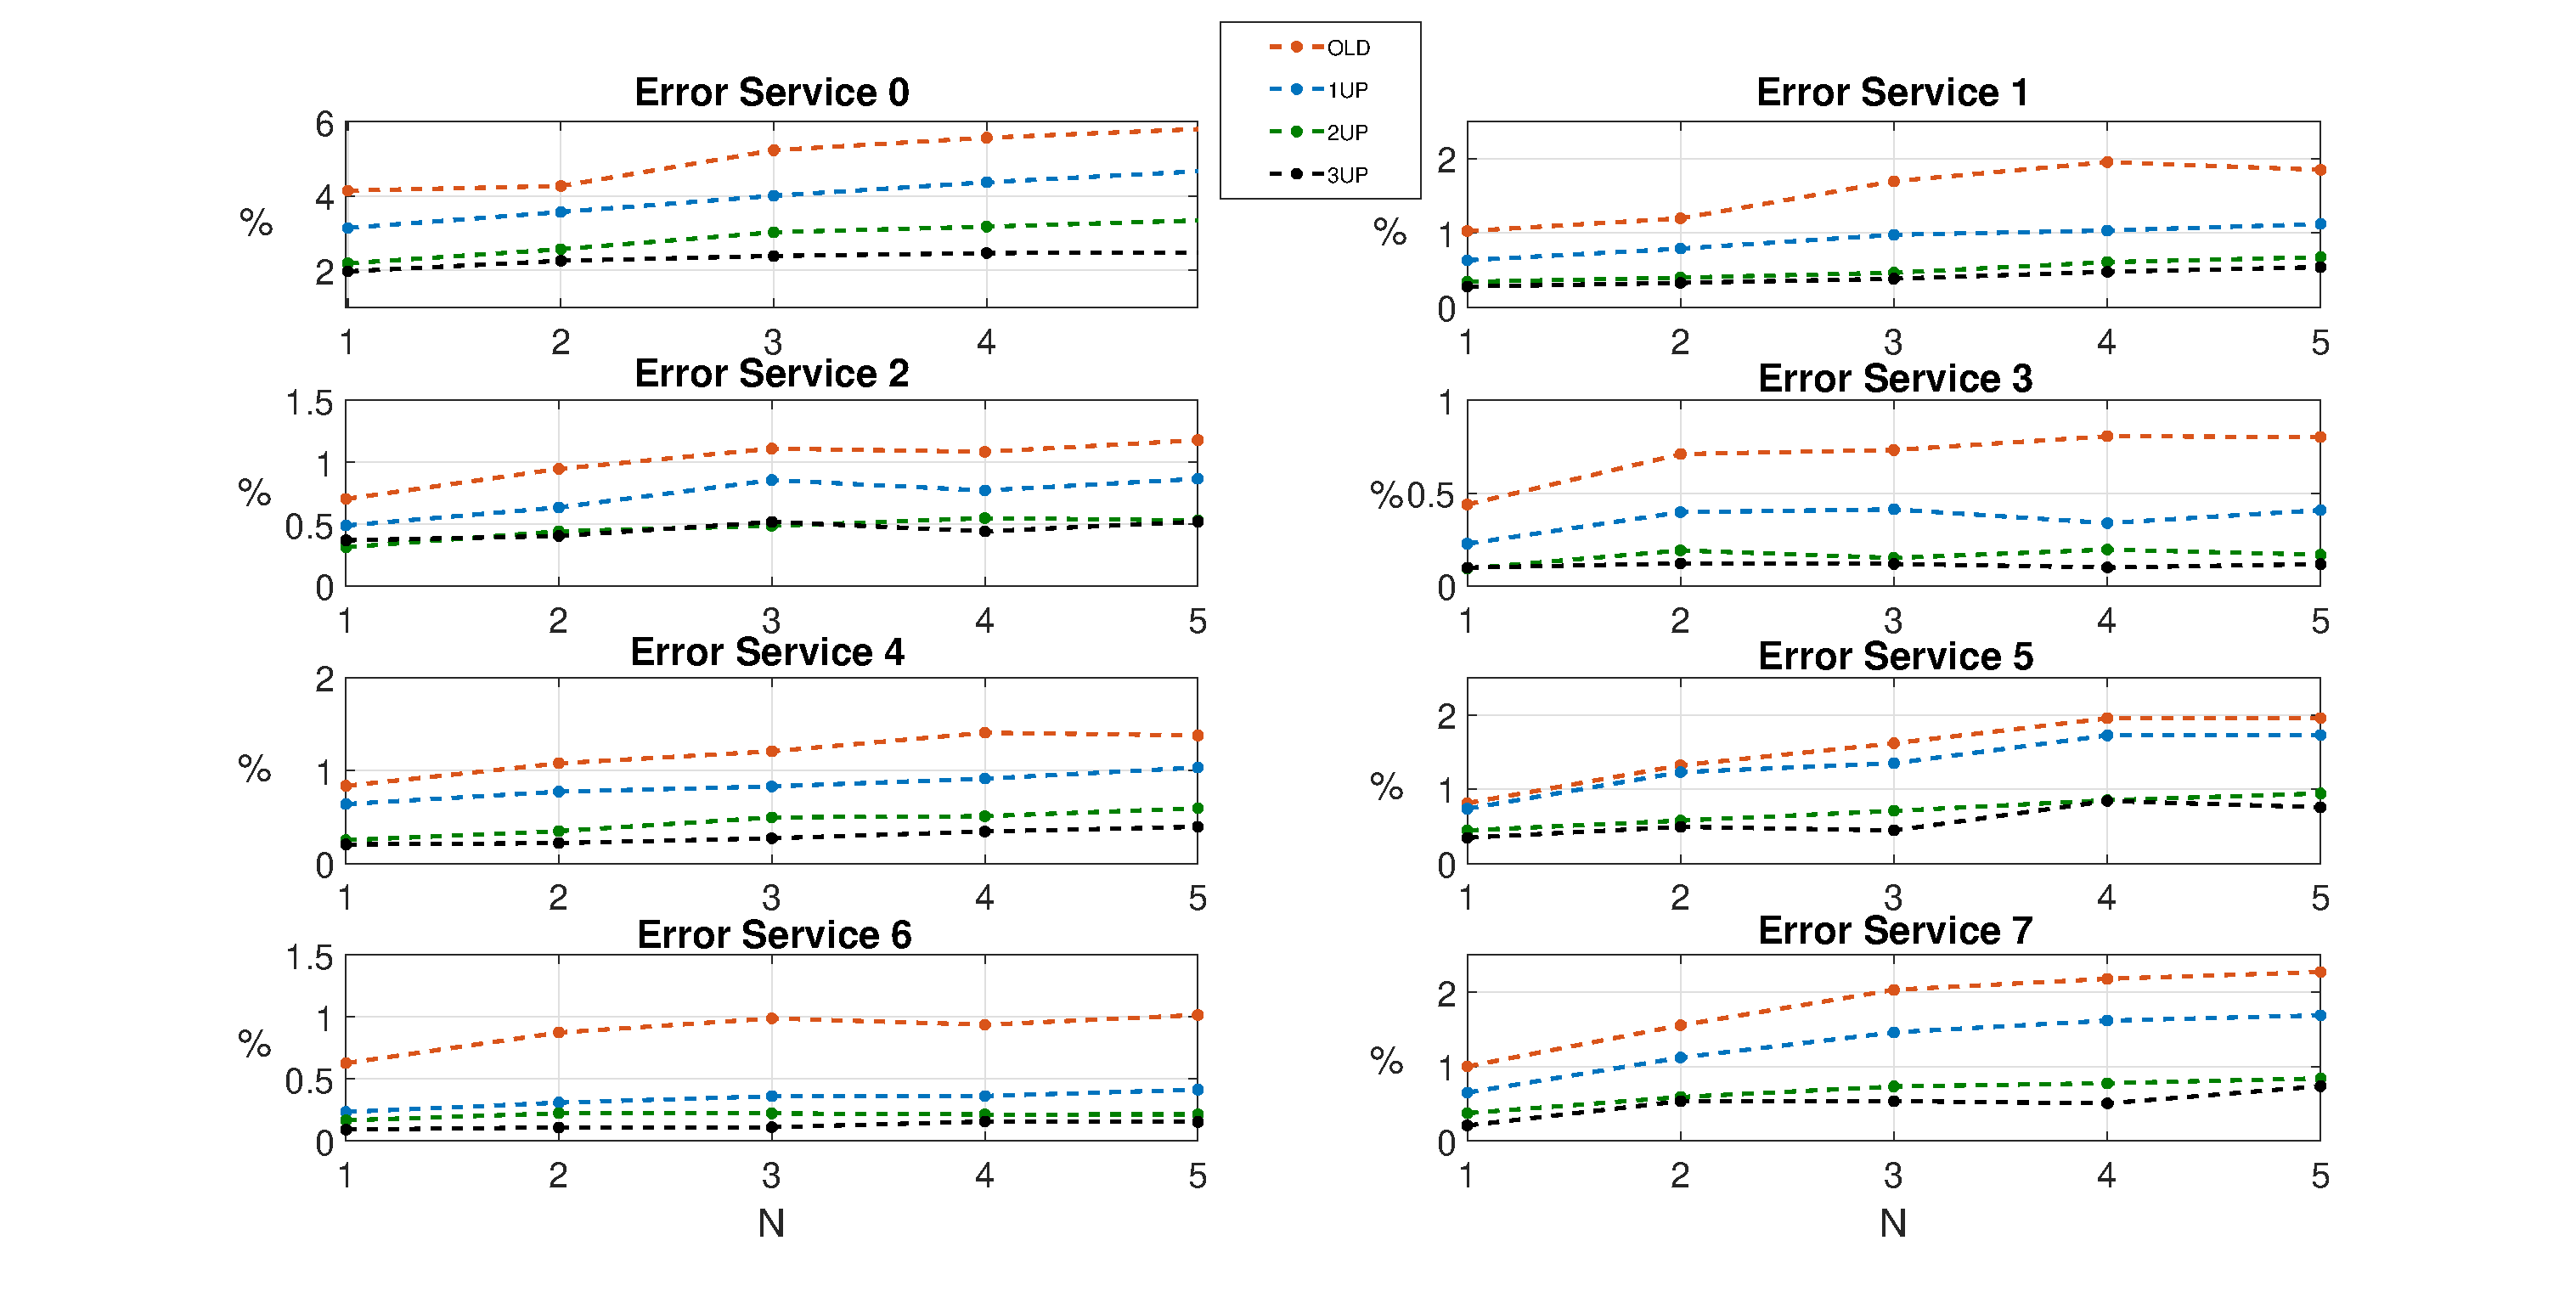
\includegraphics[trim={120 0 120 0}, width=1\linewidth]{figure/Error_Disturbance.eps}
	\caption{NRMSE of the disturbance predictive model over a time horizon of $N=5$.}
	\label{fig:{errorDist}}
\end{figure}
\begin{figure}[h!]
	\centering
	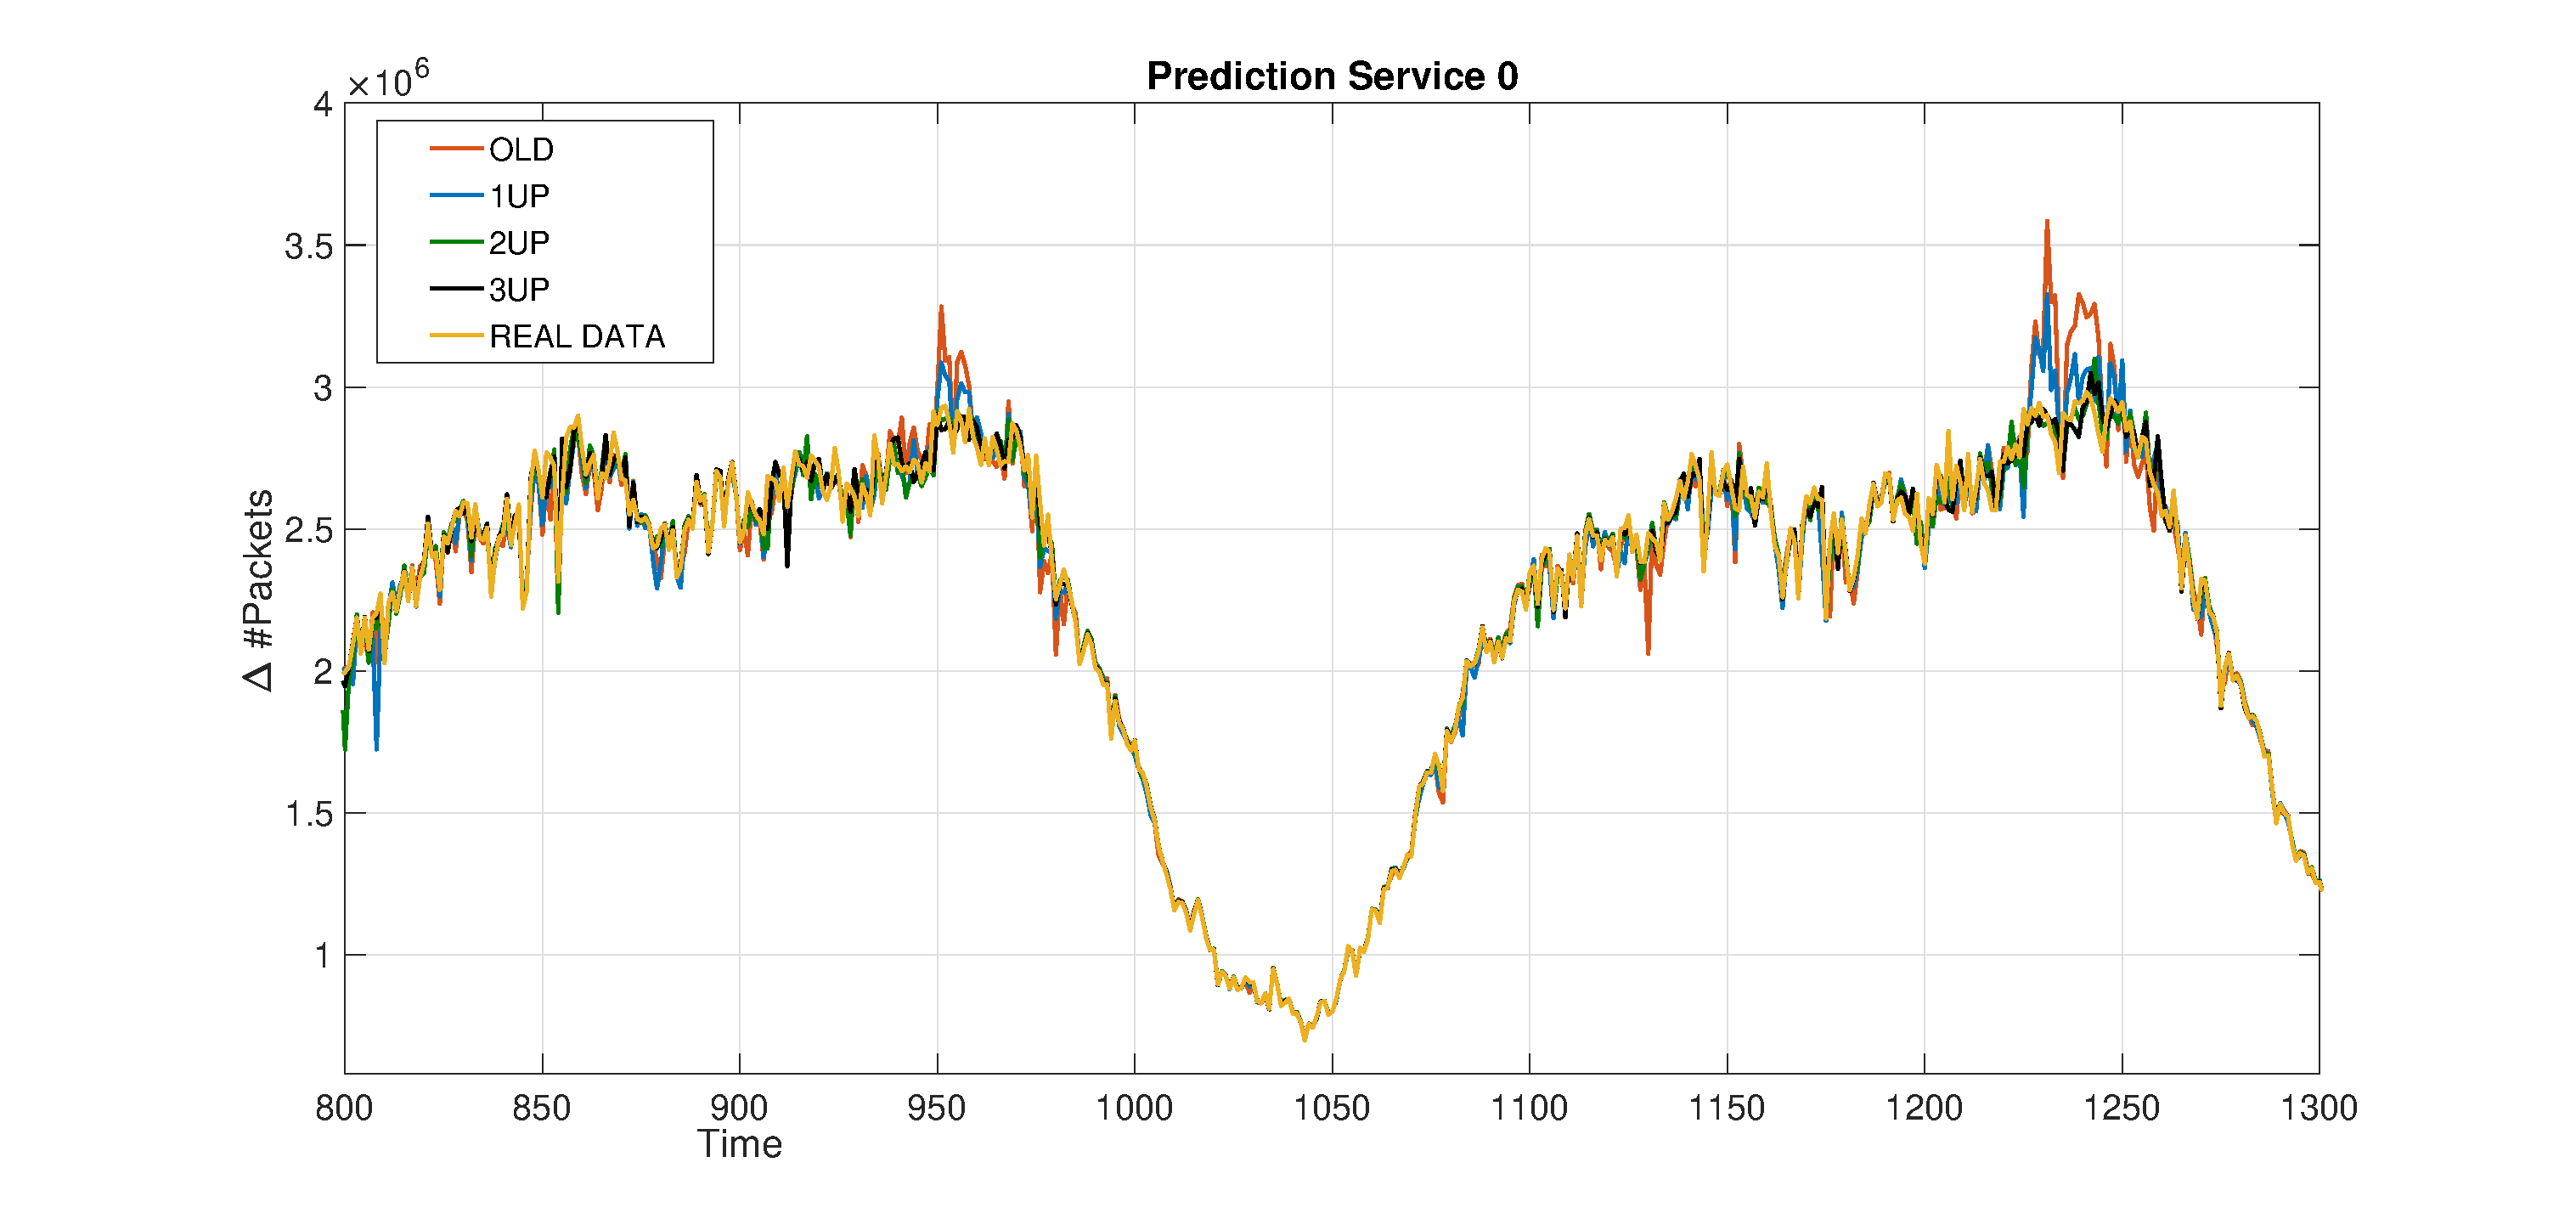
\includegraphics[trim={120 0 120 0}, width=1\linewidth]{figure/Error_Disturbance_Packets.eps}
	\caption{Comparison between the real traffic (YELLOW LINE) and the traffic prediction for the different models for Service 0.}
	\label{fig:{errorPack}}
\end{figure}

Figure \ref{fig:{errorDist}} shows the Normalised Root Mean Square Error (NRMSE) of the predictive model of the disturbance signals (one for each of the 8 DSCP indices) over a time horizon of $N=5$: the prediction error is worse for Service $0$ ($4-6\%$) since it includes the majority of the packets that transit through the switch. For other services the NRMSE is at most $2.2\%$ (Service 7) over all the predictive horizons. The improvement of the model accuracy when using larger (updated) data sets is evident, until a \textit{saturation} is reached and further data do not help to improve the model accuracy: the NRMSE significantly reduces and for Service 0 it is even halved. Figure \ref{fig:{errorPack}} plots, for Service $0$ and in a time window of $500$ samples (almost two days), the predictions of OLD, 1UP, 2UP and 3UP as well as the original data, and clearly highlights the better prediction of 2UP and 3UP with respect to OLD and 1UP.

%====================================================================================================
\subsection{Traffic predictive model validation on real network data}

{In addition to the validation of our predictive models of the incoming traffic over the Mininet environment, the accuracy has been also tested on data measured from a real network device (Ubiquiti EP-16) of an Italian internet internet provider (Sonicatel S.r.l.). Data collection has been performed using the software Cacti \cite{Cacti}.\\
Since this device is part of a running commercial network, some constraints in data collection have forced to only measure the sum of all packets entering and leaving the device, and it has been possible to extract from such traffic only incoming VOIP packets: i.e., it has not been possible to extract packets differentiated for each DSCP. Moreover, it is not currently possible to apply any type of closed-loop control on the network device. For the above 2 reasons the control performance validation in the following sections is not based on this real traffic dataset.\\
About data analysis, 53 days of data measurements have been used for RF training and about 3 days for model validation. Figure \ref{fig:{errorPescara}} shows the prediction on three classes of packets: all packets received, all packets transmitted, VOIP packets received. The plots show that our methodology provides a very accurate prediction even on a real internet service provider network.}
\begin{figure}[h!]
	\centering
	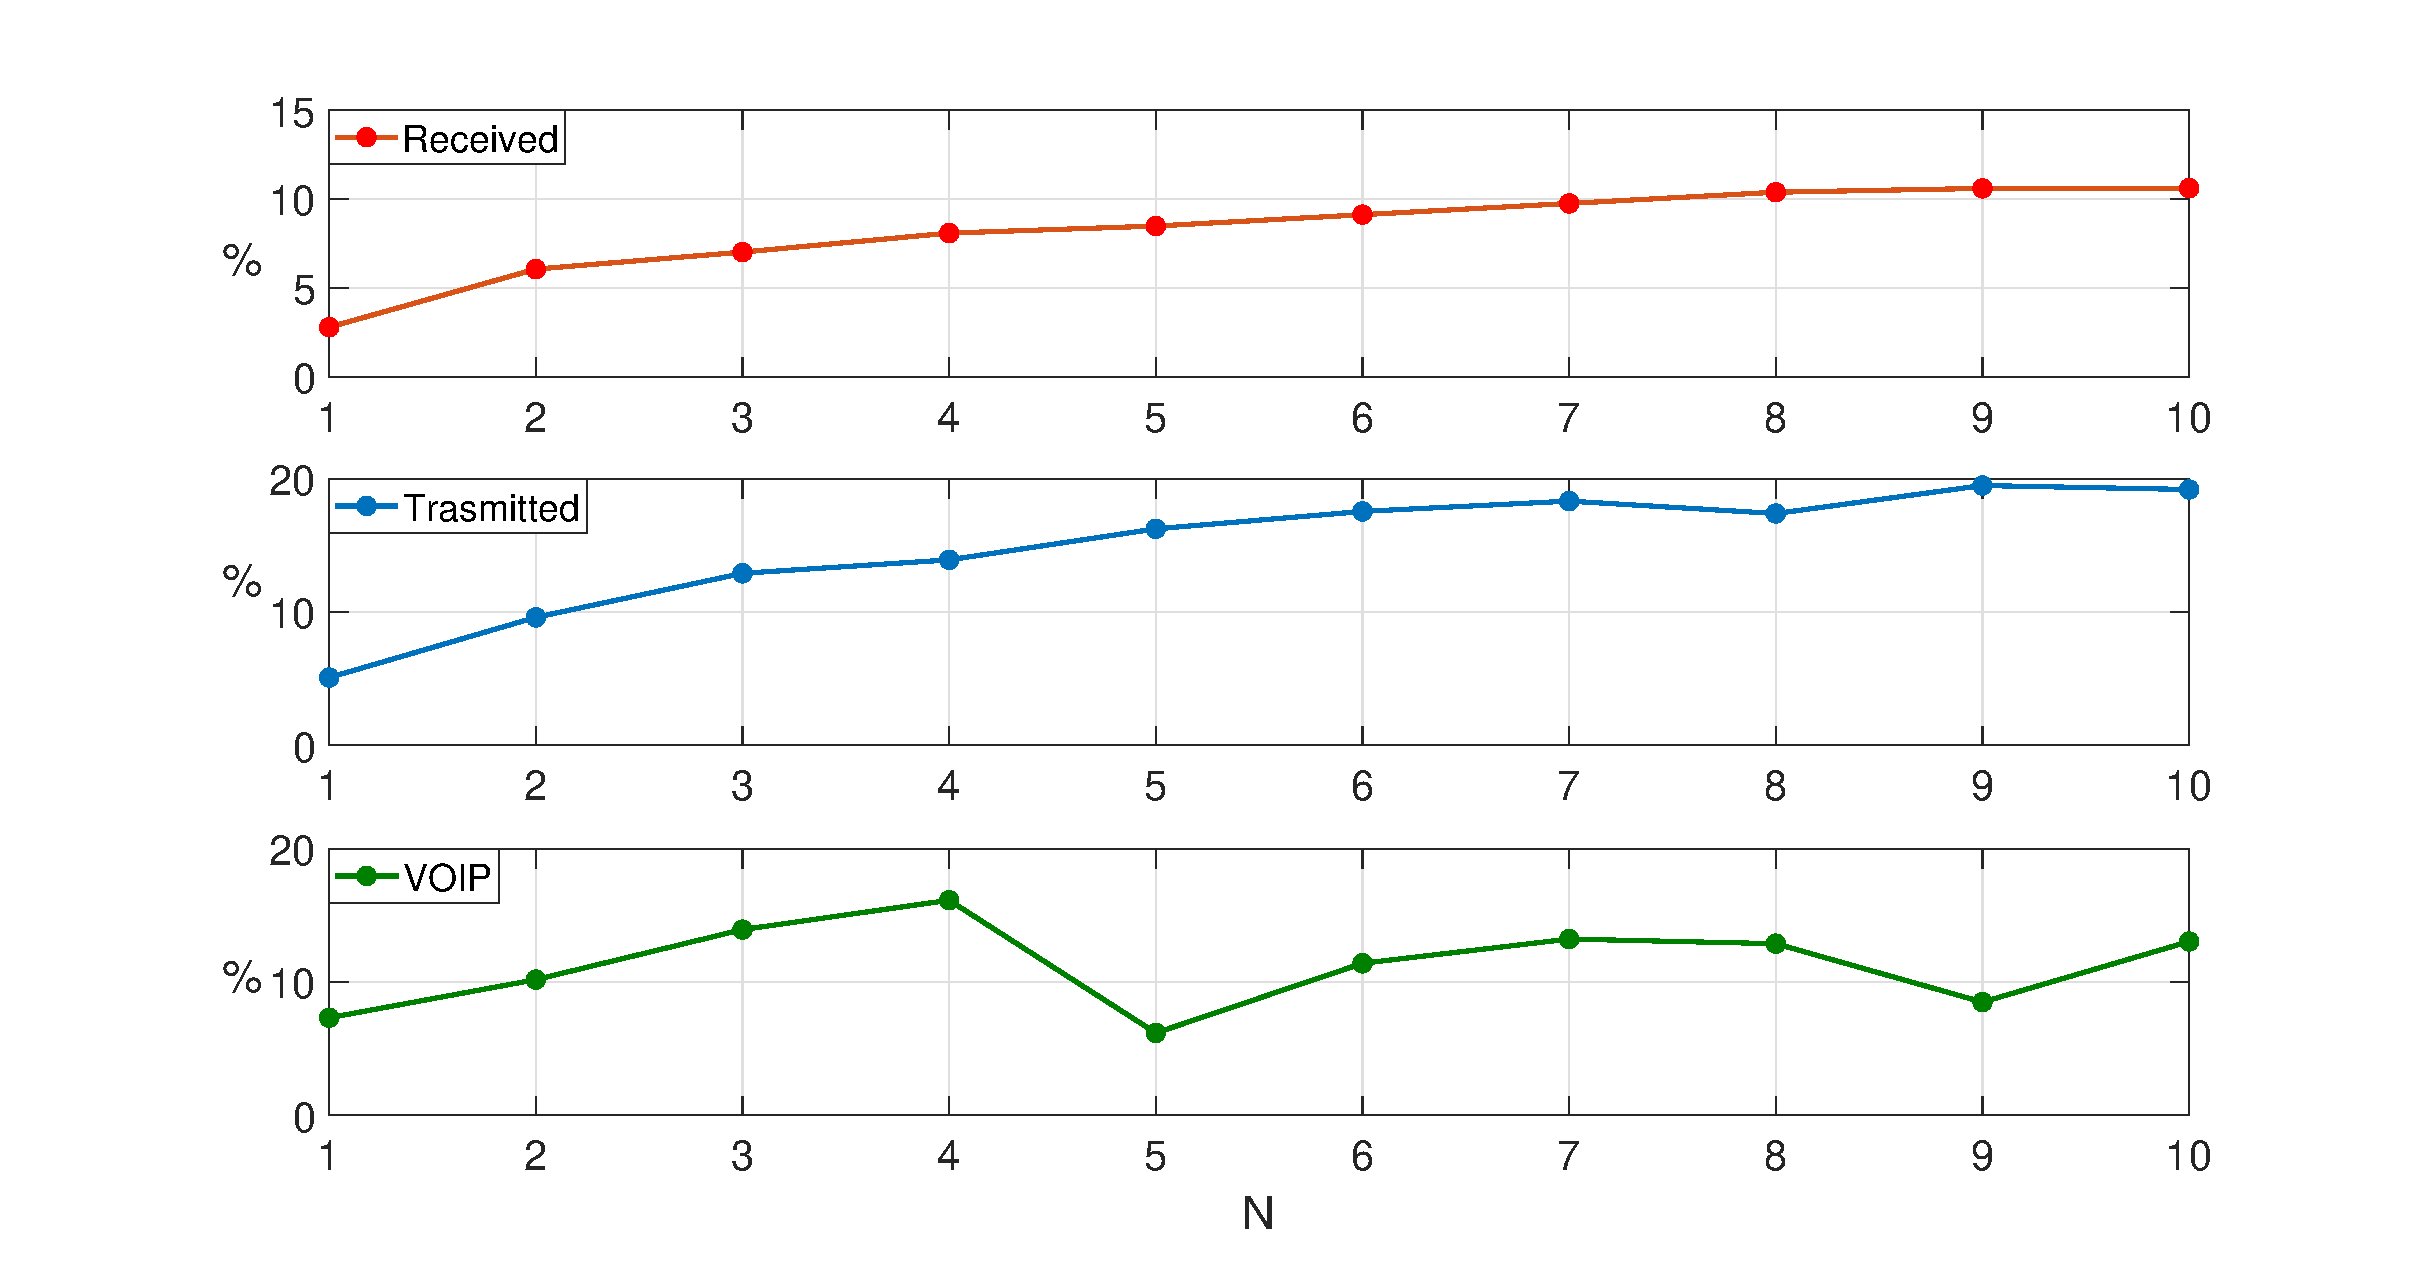
\includegraphics[trim={120 0 120 0}, width=1\linewidth]{figure/Error_PESCARA_DATA.eps}
	\caption{NRMSE of the packets predictive model over a time horizon of $N=10$.}
	\label{fig:{errorPescara}}
\end{figure}
\subsection{Queues predictive model validation}

In this section a comparison of the accuracy of RT and RF predictive models with Artificial Neural Networks will be showed. A neural network is a collection of algorithms that identify underlying relations in a dataset: it consists of groups of connected neurons organized in layers, where the connections between neurons are modeled using weights. The signal produced with this linear composition is then fed into an activation function that is in general nonlinear. The reader is referred to \cite{NNstateOfART} and references therein for more details. A wide number of tools to build Neural Networks have been developed during recent years, e.g. \cite{tensorflow2015,chollet2015keras,openNN} just to mention a few: in this work it is exploited the Deep Learning Toolbox of Matlab to compare predictive models based on NNs with the methodology proposed in this paper, based on ARX combined RTs and RFs. It is considered here just OLD as the learning dataset and a predictive horizon $N=5$.

To identify a RT (resp. RF) based predictive model of the queues it is trained a Regression Tree (resp. Random Forest) for each output and for each time horizon, with a total of $15$ trees (resp. $15$ forests each consisting of $30$ trees). The main parameters used for the identification algorithm (see Section \ref{secSwitchedModeling} and Problem \ref{pbLeastSquareProblem}) are summarized in Table \ref{tab:idPar}.  
\begin{table}[h!]
	\caption{Identification parameters}
	\centering
	\begin{tabular}{l c l c}
		\hline\hline
		Parameters & Value & Parameters & Values\\ 
		\hline
		N          & 5   & $f_{min}$  & -100 \\
		$\delta_y$ & 1   & $f_{max}$  & 100  \\
		$\delta_x$ & 5   & $a_{min}$  & -100  \\
		$\delta_u$ & 0   & $a_{max}$  & 100 \\
		$\delta_d$ & 5   & $b_{min}$  & 0  \\
		$\delta$   & 5   & $b_{max}$  & 10000  \\
		$|\Fij|$   & 30  & Minleaf    & 13\\
		\hline
	\end{tabular}
	\label{tab:idPar}
\end{table}
{In particular, as done with $\delta$ in Equation \eqref{eqIdentifiedModelN}, parameters $\delta_x$ and $\delta_d$ are considered as regressive terms of the state and disturbance that will be only used to grow the trees and the forests, i.e. $\sigma_j(k) = \sigma_j(x(k),\ldots,x(k-\delta_x),\bold{u^-}(k),d(k),\ldots,d(k-\delta_d))$. The regressive terms ($\delta_d$, $\delta_y$, $\delta_x$, $\delta_u$, $\delta$)} and the minimum number of samples for each tree of each forest (MinLeaf) have been chosen, with a trial and error approach, considering that very small regressive horizons and very large values for MinLeaf may lead to inaccurate prediction (as they do not provide sufficient information on the past) but very large regressive horizons and very small values for MinLeaf also lead to inaccurate prediction (as they interpolate very old data that might negatively affect the results and produce overfitting).

Regarding specific parameters used for running NN, and for the sake of a fair comparison, they have been tuned to obtain the best performance: in particular shallow networks of 2 layers are considered since deeper networks did not improve the accuracy and, instead, have the negative effect of increasing the sensitivity of the accuracy with respect to the initial conditions of the weights. Among the many algorithms for optimizing the weights of the neurons, the following will be considered: \textit{Scaled conjugate gradient back-propagation} described in \cite{Moller1990}, which provided the best accuracy with respect to the dataset considered. Regarding the activation functions, both the classical sigmoid function (\textit{LogSig}) and the Hyperbolic tangent sigmoid transfer function (\textit{TanSig}) are used.
\begin{figure}[h!]
	\centering
	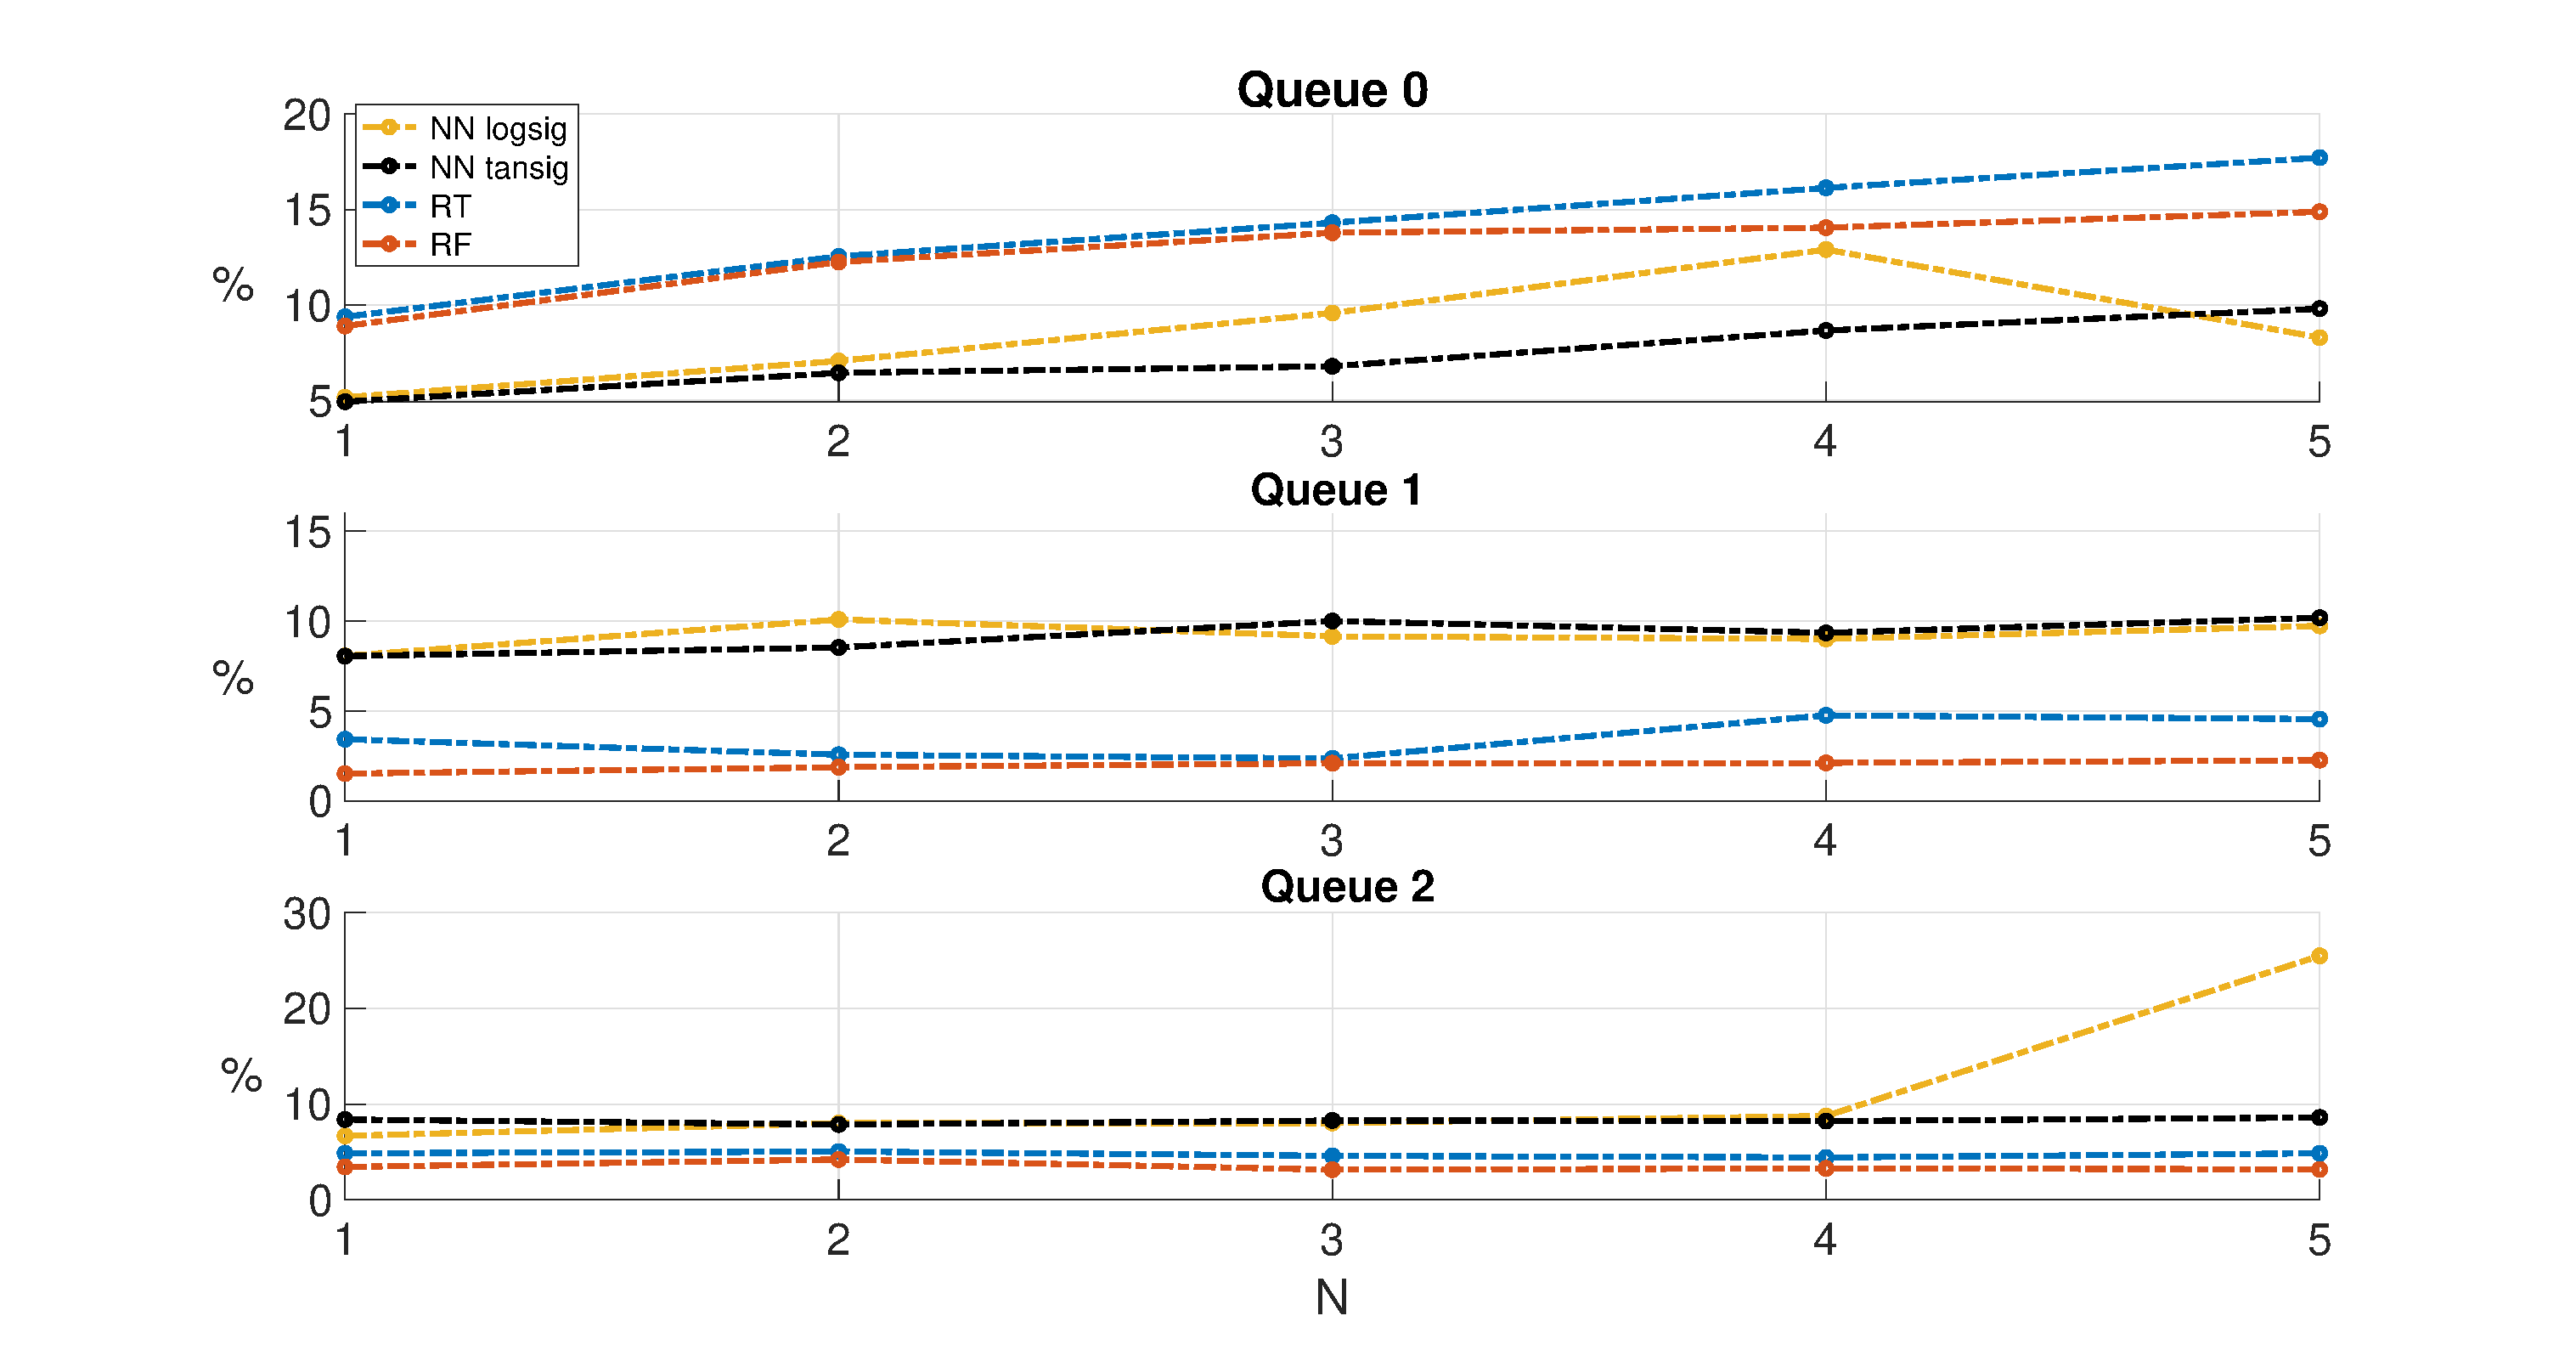
\includegraphics[trim={120 0 120 0},width=0.9\linewidth]{figure/NRMSENNvsRTvsRF.eps}
	\vspace{-0.2cm}
	\caption{NRMSE, up to $N=5$ and for each priority class, for RT (blue), RF (red), NN with sigmoids as activation function (yellow) and NN with hyperbolic tangent as activation function (black).}
	\label{fig:{NRMSE}}
\end{figure}

As a metric of the prediction accuracy in Figure \ref{fig:{NRMSE}} is shown a comparison between the Normalized Root Mean Square Errors (NRMSE) of the different identification approaches for each priority class and over a horizon up to $N=5$. Regarding queue $0$ (Default) NNs perform better than RT and RF, but in queues $1$ (Premium) and $2$ (Gold), characterised by higher priority, RF provides the best performance. Queue $0$ is characterised by a larger NRMSE with all identification techniques: this is due to the fact that, having the lowest priority, it suffers more packet losses and this can negatively affect the prediction accuracy. The validation emphasizes that RTs, even thought very simple and fast to compute, are often affected by overfitting and variance issues, i.e. small variations of the training data result in large variations of the tree structure and, consequently, of the predictions. Regarding NNs, they provide a less accurate model in 2 cases over 3. Indeed, by analyzing the dataset distribution, it is possible to notice a peculiar regular grid pattern that can be very well approximated by hyper-rectangles: since RTs and RFs base their prediction on hyper-rectangular dataset partitions, the better performance with respect to NNs is reasonable. For queue 0, even thought NNs perform better, it is important to remark that their predictive model is based on nonlinear functions: this makes the derived model impractical for real-time control as the corresponding MPC formulation turns into a nonlinear optimization problem, for which there is no approach that can guarantee neither a global optimal solution nor a reasonable computation time. In addition to this, even obtaining a closed mathematical form of the predictive function of a Neural Network starting from neurons and weights is not always an easy task, because of the highly nonlinear interconnections between the different layers. For all these reasons it will be only used, from now on, RF-based models which provide the best choice both from the accuracy and the computational complexity points of view. In the following it is illustrated the effect of iterative dataset updates in the prediction accuracy, both with and without prediction of the future disturbances.
\begin{figure}[th!]
	\centering
	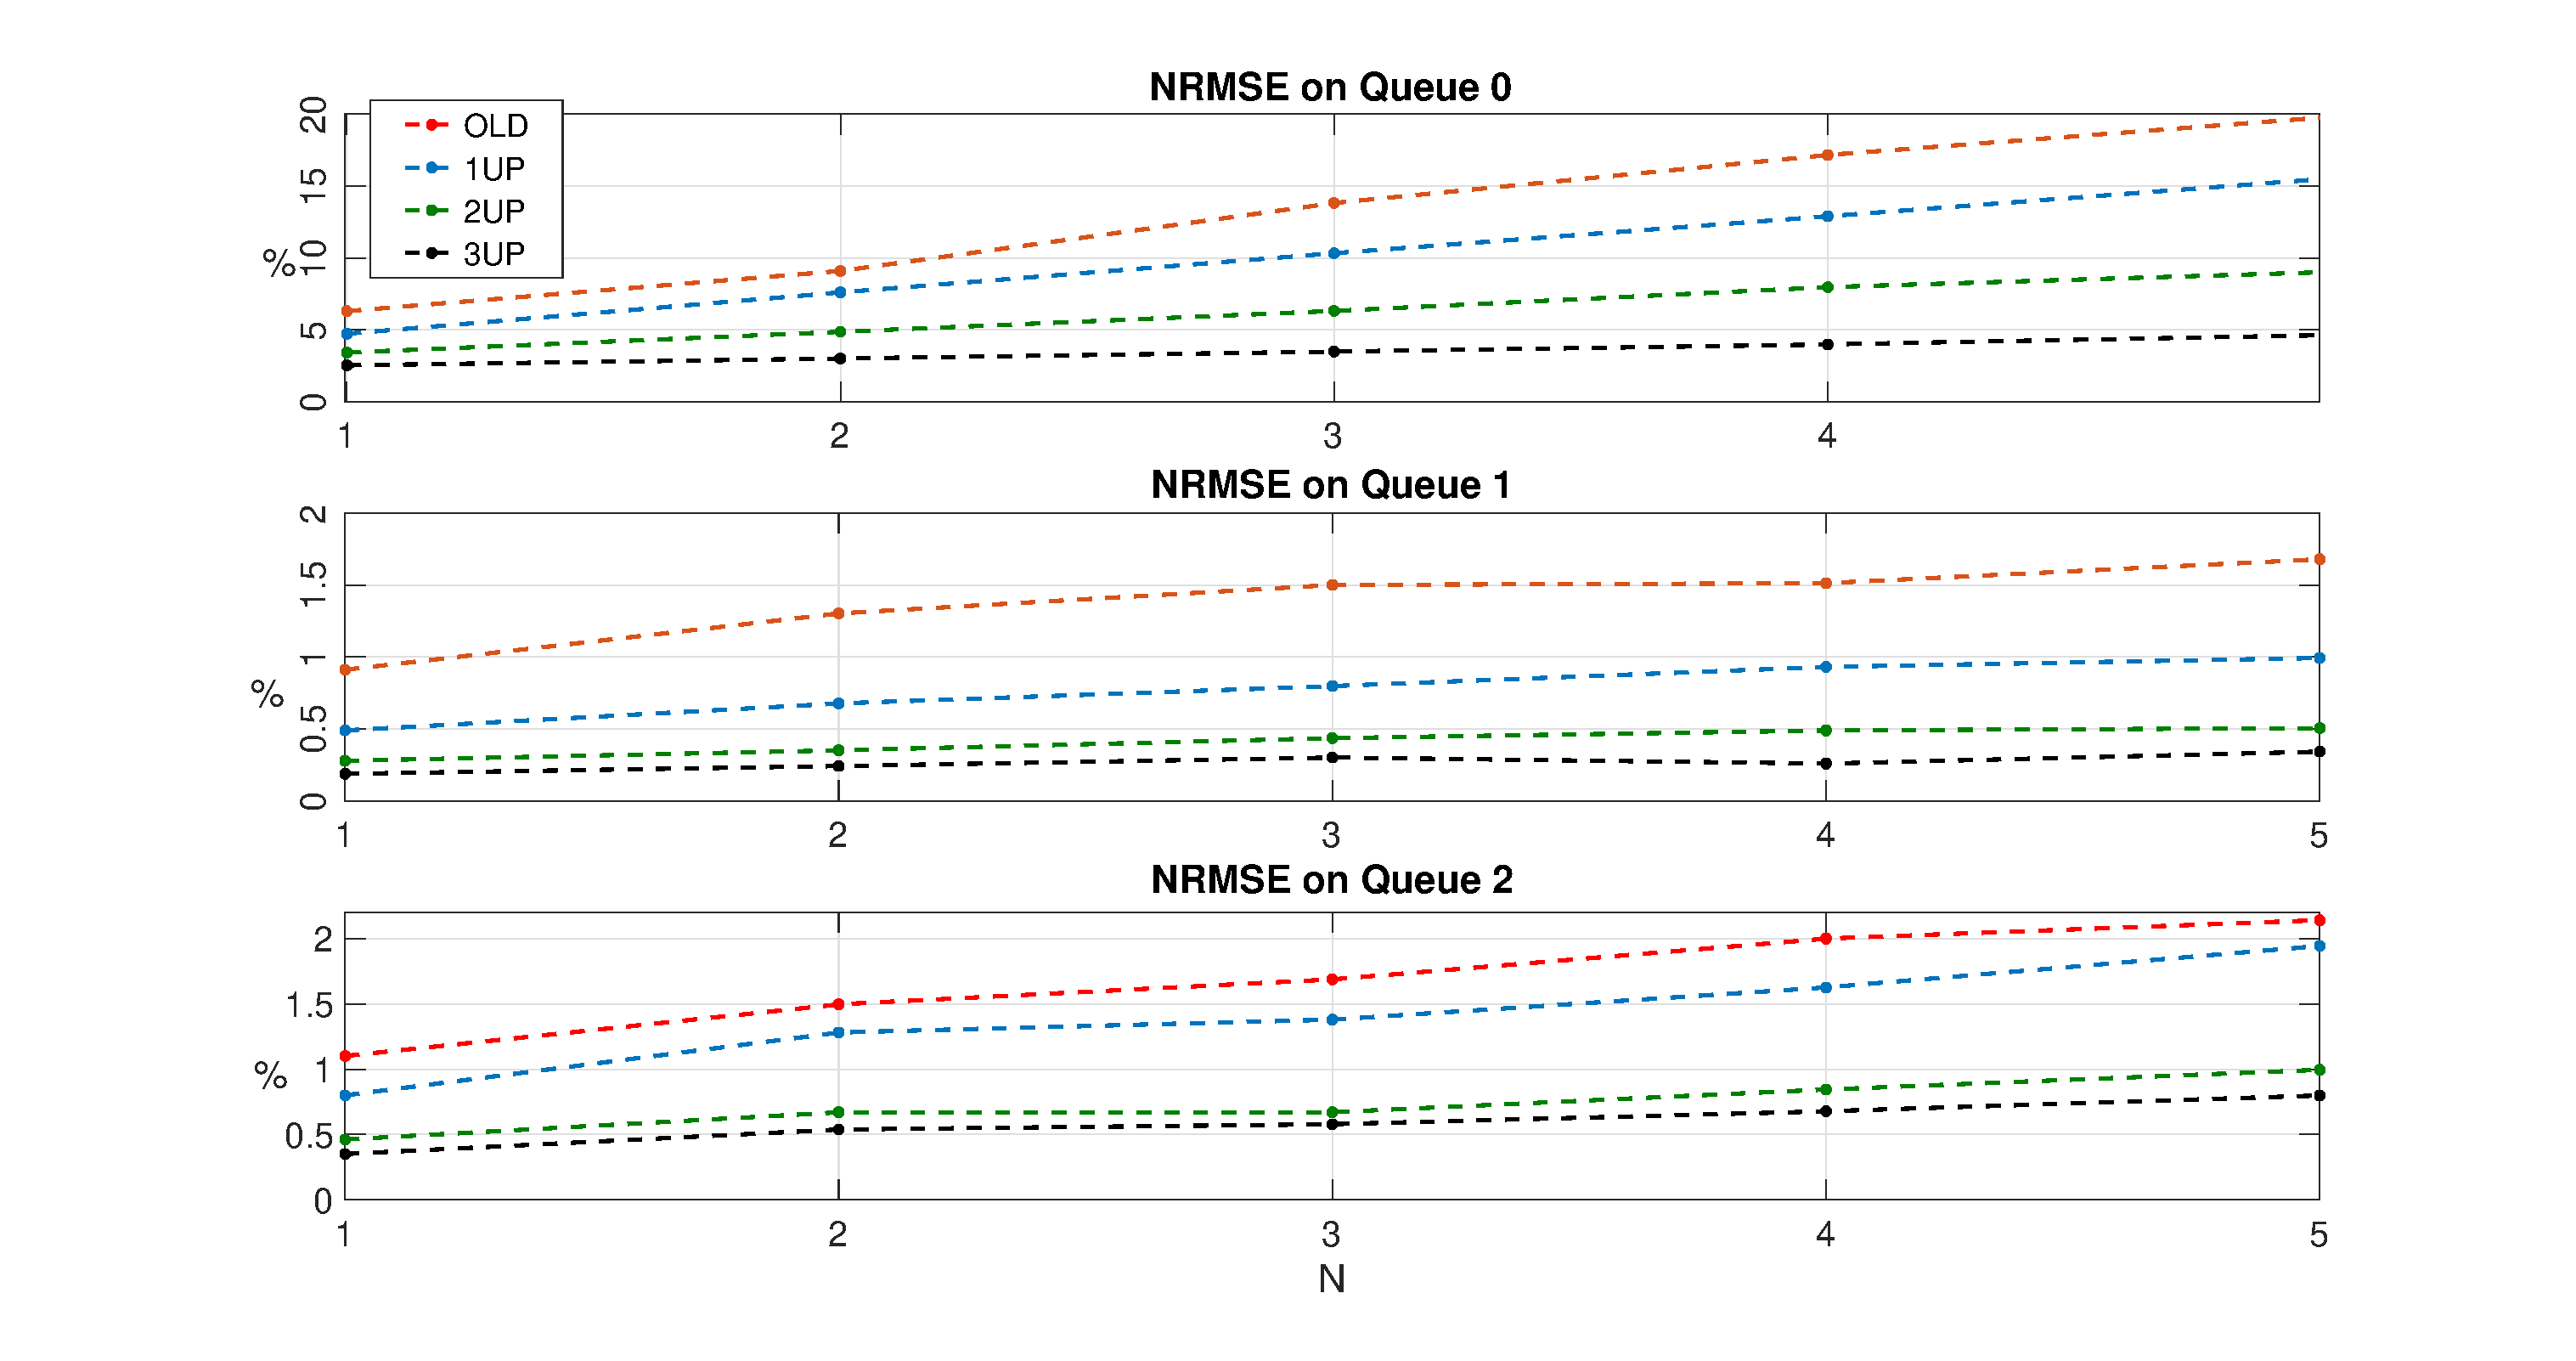
\includegraphics[trim={120 0 120 0}, width=0.9\linewidth]{figure/Error_State.eps}
	\caption{NRMSE of the queues output predictive model over a time horizon of $N=5$, without prediction of the future disturbances}
	\label{fig:{stateNRMSE}}
\end{figure}
\begin{figure}[th!]
	\centering
	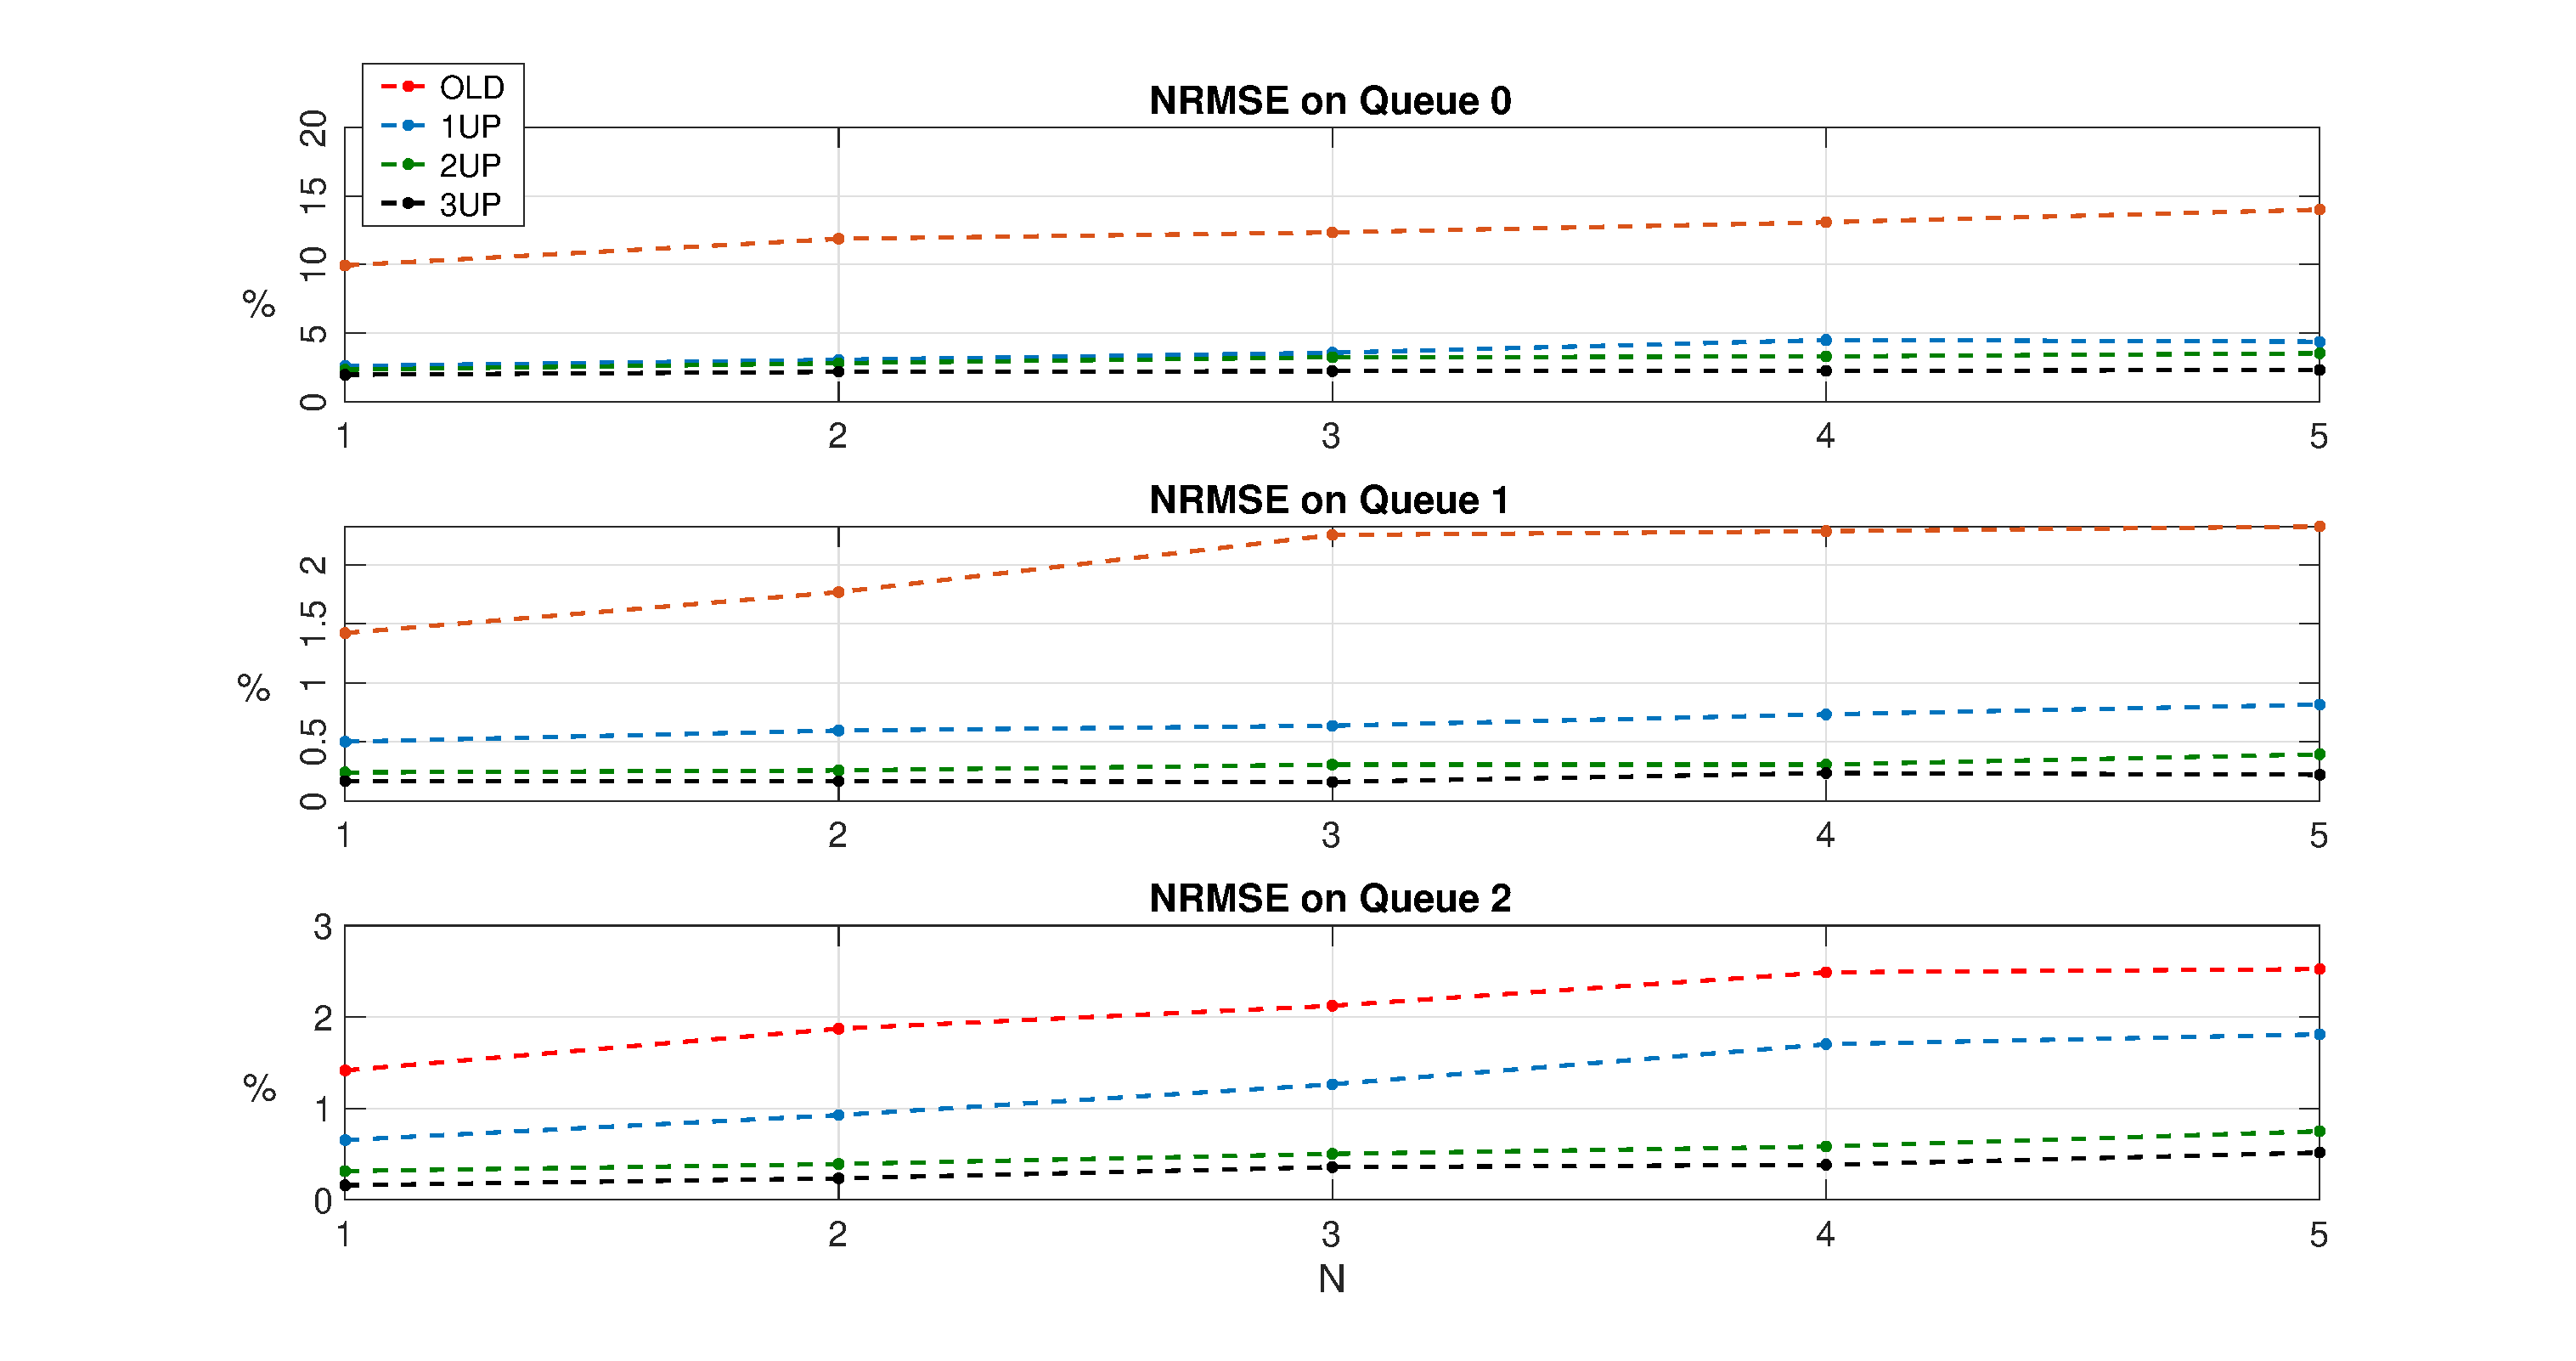
\includegraphics[trim={120 0 120 0}, width=0.9\linewidth]{figure/Error_State_ddM4.eps}
	\caption{NRMSE of the queues output predictive model over a time horizon of $N=5$, with prediction of the 4-steps future disturbances}
	\label{fig:{stateNRMSEddM4}}
\end{figure}

Figure \ref{fig:{stateNRMSE}} and Figure \ref{fig:{stateNRMSEddM4}} plot the NRMSEs respectively without and with prediction of the future disturbances. The assumption of future disturbance forecast, as expected, provides much better prediction accuracy. The positive effect of updated data sets is also clear, providing accuracy improvements up to $50 \%$: as will be also discussed in the next section, the most relevant prediction accuracy improvement takes place moving from OLD to 1UP or from 1UP to 2UP, while the 3UP model does not improve much.

\begin{remark}
In the simulations shown in this work, data are generated without major modifications of the traffic daily pattern: for this reason enriching the data set converges to a saturation of the model accuracy, as discussed above. Nevertheless, the capability of the proposed methodology to iteratively learn from new data is fundamental as, in real life, changes in the traffic patterns do occur, and model updates are necessary to maintain the model accuracy and the control performance. 
\end{remark}

%====================================================================================================

\subsection{Control performance}

In this section a control loop is setup, where the (Mininet) network emulator and the (Ryu) controller run in two different computers, and synchronize/exchange data using a shared file. Namely, the SW controller module is ready to be directly used on a real SDN-based network, with just some minor modifications in the data exchange with the switch devices. The controller implements MPC using the predictive models validated in the previous sections: at each time step, it solves Problem \ref{pbMPC} and optimally updates the bandwidth of the different queues. The cost matrices $Q$ and $R$ of Problem \ref{pbMPC} respectively weight the output $y(k)$ of the system (i.e. the packet transmission rate for each queue) and the control input $u(k)$ (i.e. the bandwidth assigned to each queue). Since $R$ is required to be positive definite but it makes no sense assigning a penalty to the choice of $u(k)$, the choice has been $R=10^{-5} \cdot \mathbb I$, where the identity matrix $\mathbb I$ multiplies a very small value. Matrix $Q = diag(1,10^4,10)$ has been assigned as a diagonal matrix, where the choice of the different diagonal components is related to the priority level of each queue. The remaining constraints of Problem \ref{pbMPC} are reported in Table \ref{tab:contPar}.
%The parameters used in the constraints described in Problem \ref{pbMPC} are reported in Table \ref{tab:contPar} and the weights matrices considered in the optimisation cost are: $Q=diag([1,1000,10])$ and $R=10^{-5} \mathbb{I}_3$.
\begin{table}[h!]
	\caption{Constraints in Problem \ref{pbMPC}}
	\centering
	\begin{tabular}{l c l c}
		\hline\hline
		Parameters                                & Value               & Parameters                 & Values       \\ 
		\hline
		$\Delta u_1^\mathrm{min}$     & 1                   & $\Delta u_1^\mathrm{max}$  & 30           \\
		$\Delta u_2^\mathrm{min}$     & 20                  & $\Delta u_2^\mathrm{max}$  & 30           \\
		$\Delta u_3^\mathrm{min}$     & 20                  & $\Delta u_3^\mathrm{max}$  & 20           \\
		$u_1^\mathrm{min} $             & 10                  & $u_1^\mathrm{max} $        & 45           \\
		$u_2^\mathrm{min} $            & 55                  & $u_2^\mathrm{max} $        & 80           \\
		$u_3^\mathrm{min} $            & 80                  & $u_3^\mathrm{max} $        & 100          \\
		
		\hline
	\end{tabular}
	\label{tab:contPar}
\end{table}
In what follows it is validated the control performance both without and with prediction of the future disturbances. The values of $x_{\mathrm{ref},j}$ in the optimization problem represent the reference values chosen for tracking system output: indeed, as the objective is to minimize packet losses, it is minimized the difference between the packets received by the hosts $d(k)$ and those transmitted by the queues $y(k)$ over the horizon $N$. In case there are no prediction of future disturbances, $x_{\mathrm{ref},j}=x_{\mathrm{ref}}=d(k)$ will be equal to the current disturbance  measurement and constant over all the predictive horizon; if instead there is a prediction of future disturbances, $x_{\mathrm{ref},j}$ will be equal to such forecast. In this section are compared only models OLD, 1UP and 2UP, since model 3UP does not provide any substantial improvement. 

 \begin{figure}[h!]
	\centering
	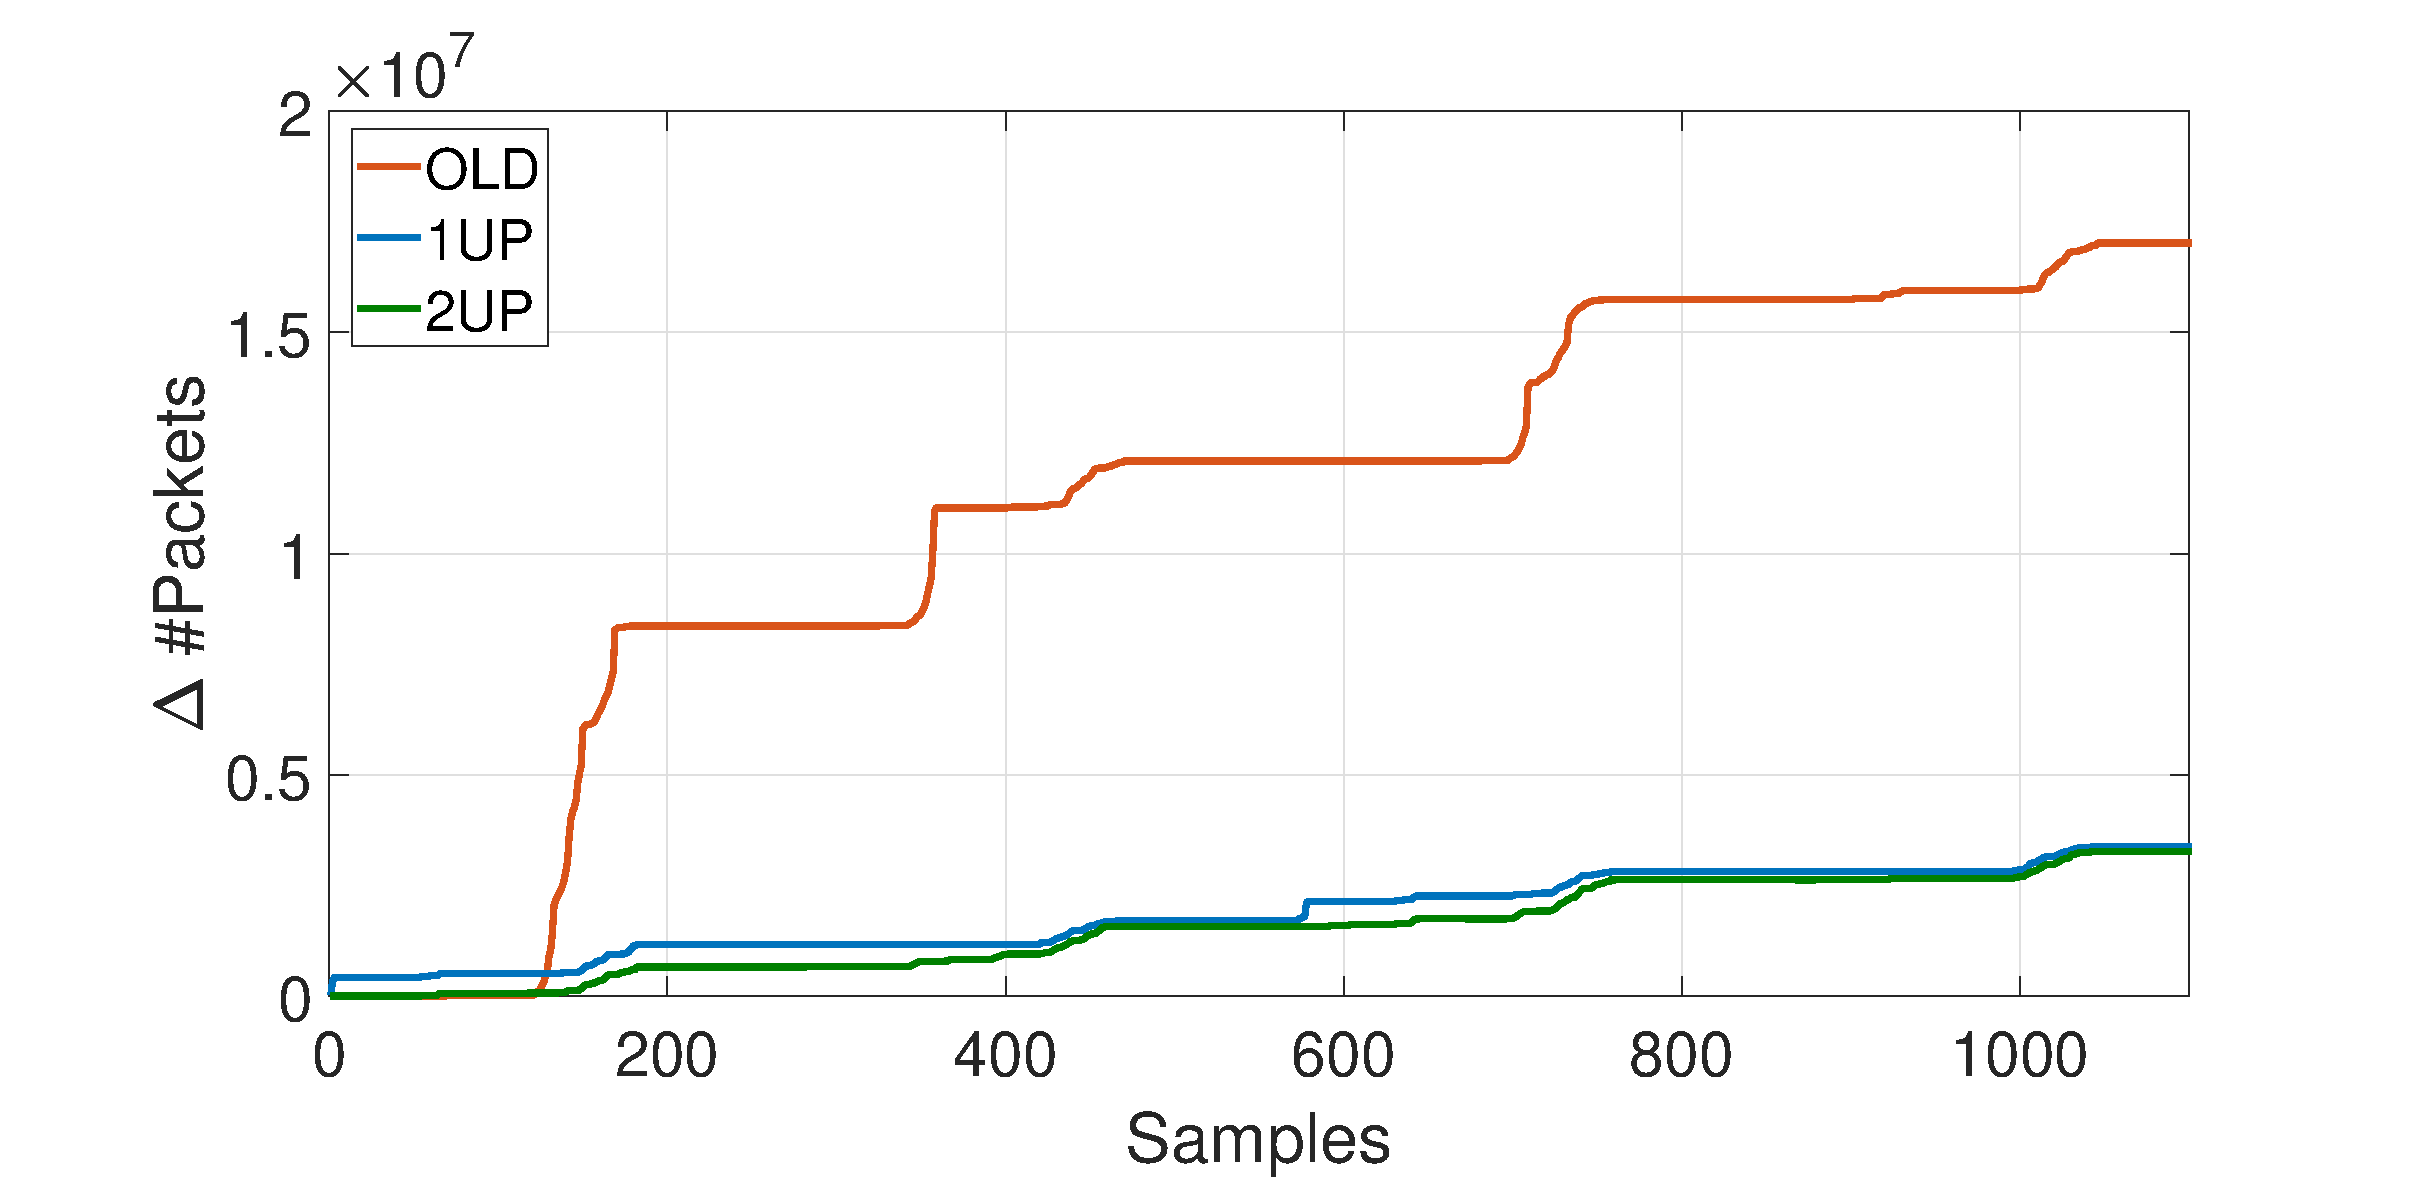
\includegraphics[trim={120 0 120 0}, width=0.9\linewidth]{figure/cumPL1.eps}
	\caption{Cumulative Packet Losses without prediction of the future disturbance.}
	\label{fig:{MPC1}}
\end{figure}
\begin{figure}[h!]
	\centering
	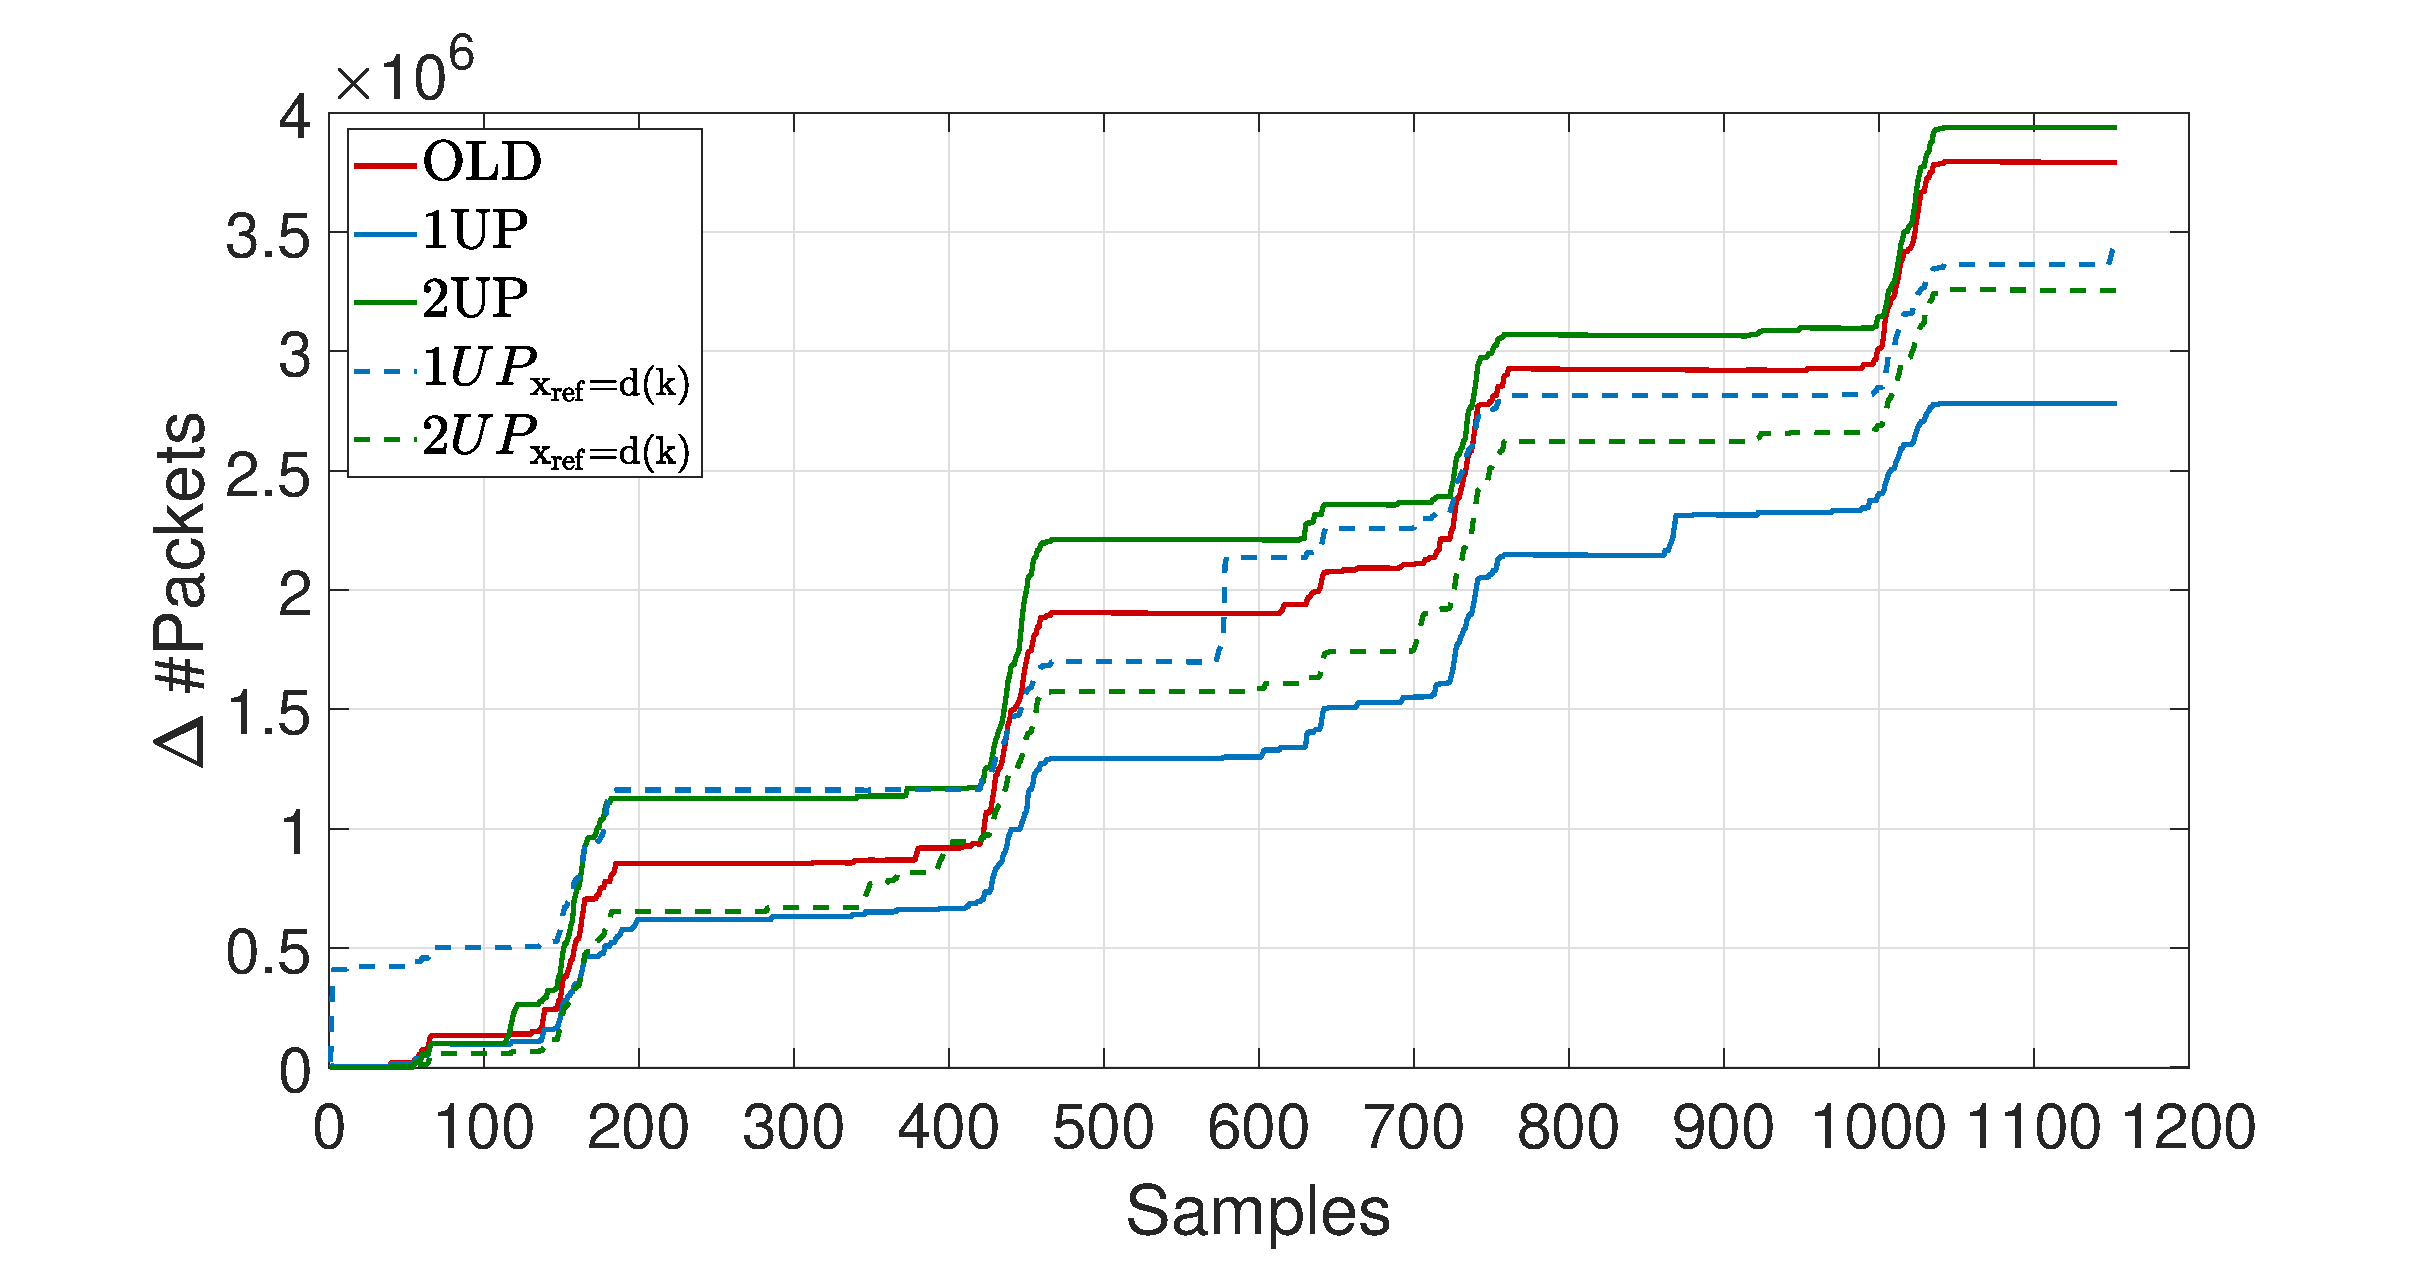
\includegraphics[trim={120 0 120 0},width=0.85\linewidth]{figure/cumPL_Total.eps}
	\caption{Comparison between Cumulative Packet Losses with (solid lines)  and without (dashed lines) prediction of the future disturbance.}
	\label{fig:{MPC2}}
\end{figure}
 Figures \ref{fig:{MPC1}} and \ref{fig:{MPC2}} plot the cumulative packet losses respectively without and with prediction of the future disturbances. The packet loss rate when the control is performed exploiting the OLD model and without disturbance forecast is around $123\%$ larger than all other cases (and, of course, incomparably smaller than the static control case \cite{Notiziario}). It is also clear from the plots that 1UP and 2UP without disturbance forecast and OLD, 1UP and 2UP with disturbance forecast provide very similar performance. Authors' interpretation is that OLD models without disturbance forecast have not enough information to provide good accuracy, but they can be easily improved either with a data set update (which however requires $10$ days for 1UP and $20$ days for 2UP of additional data) or using a predictive disturbance model.

\begin{figure}[h!]
\centering
\subfigure[a][]{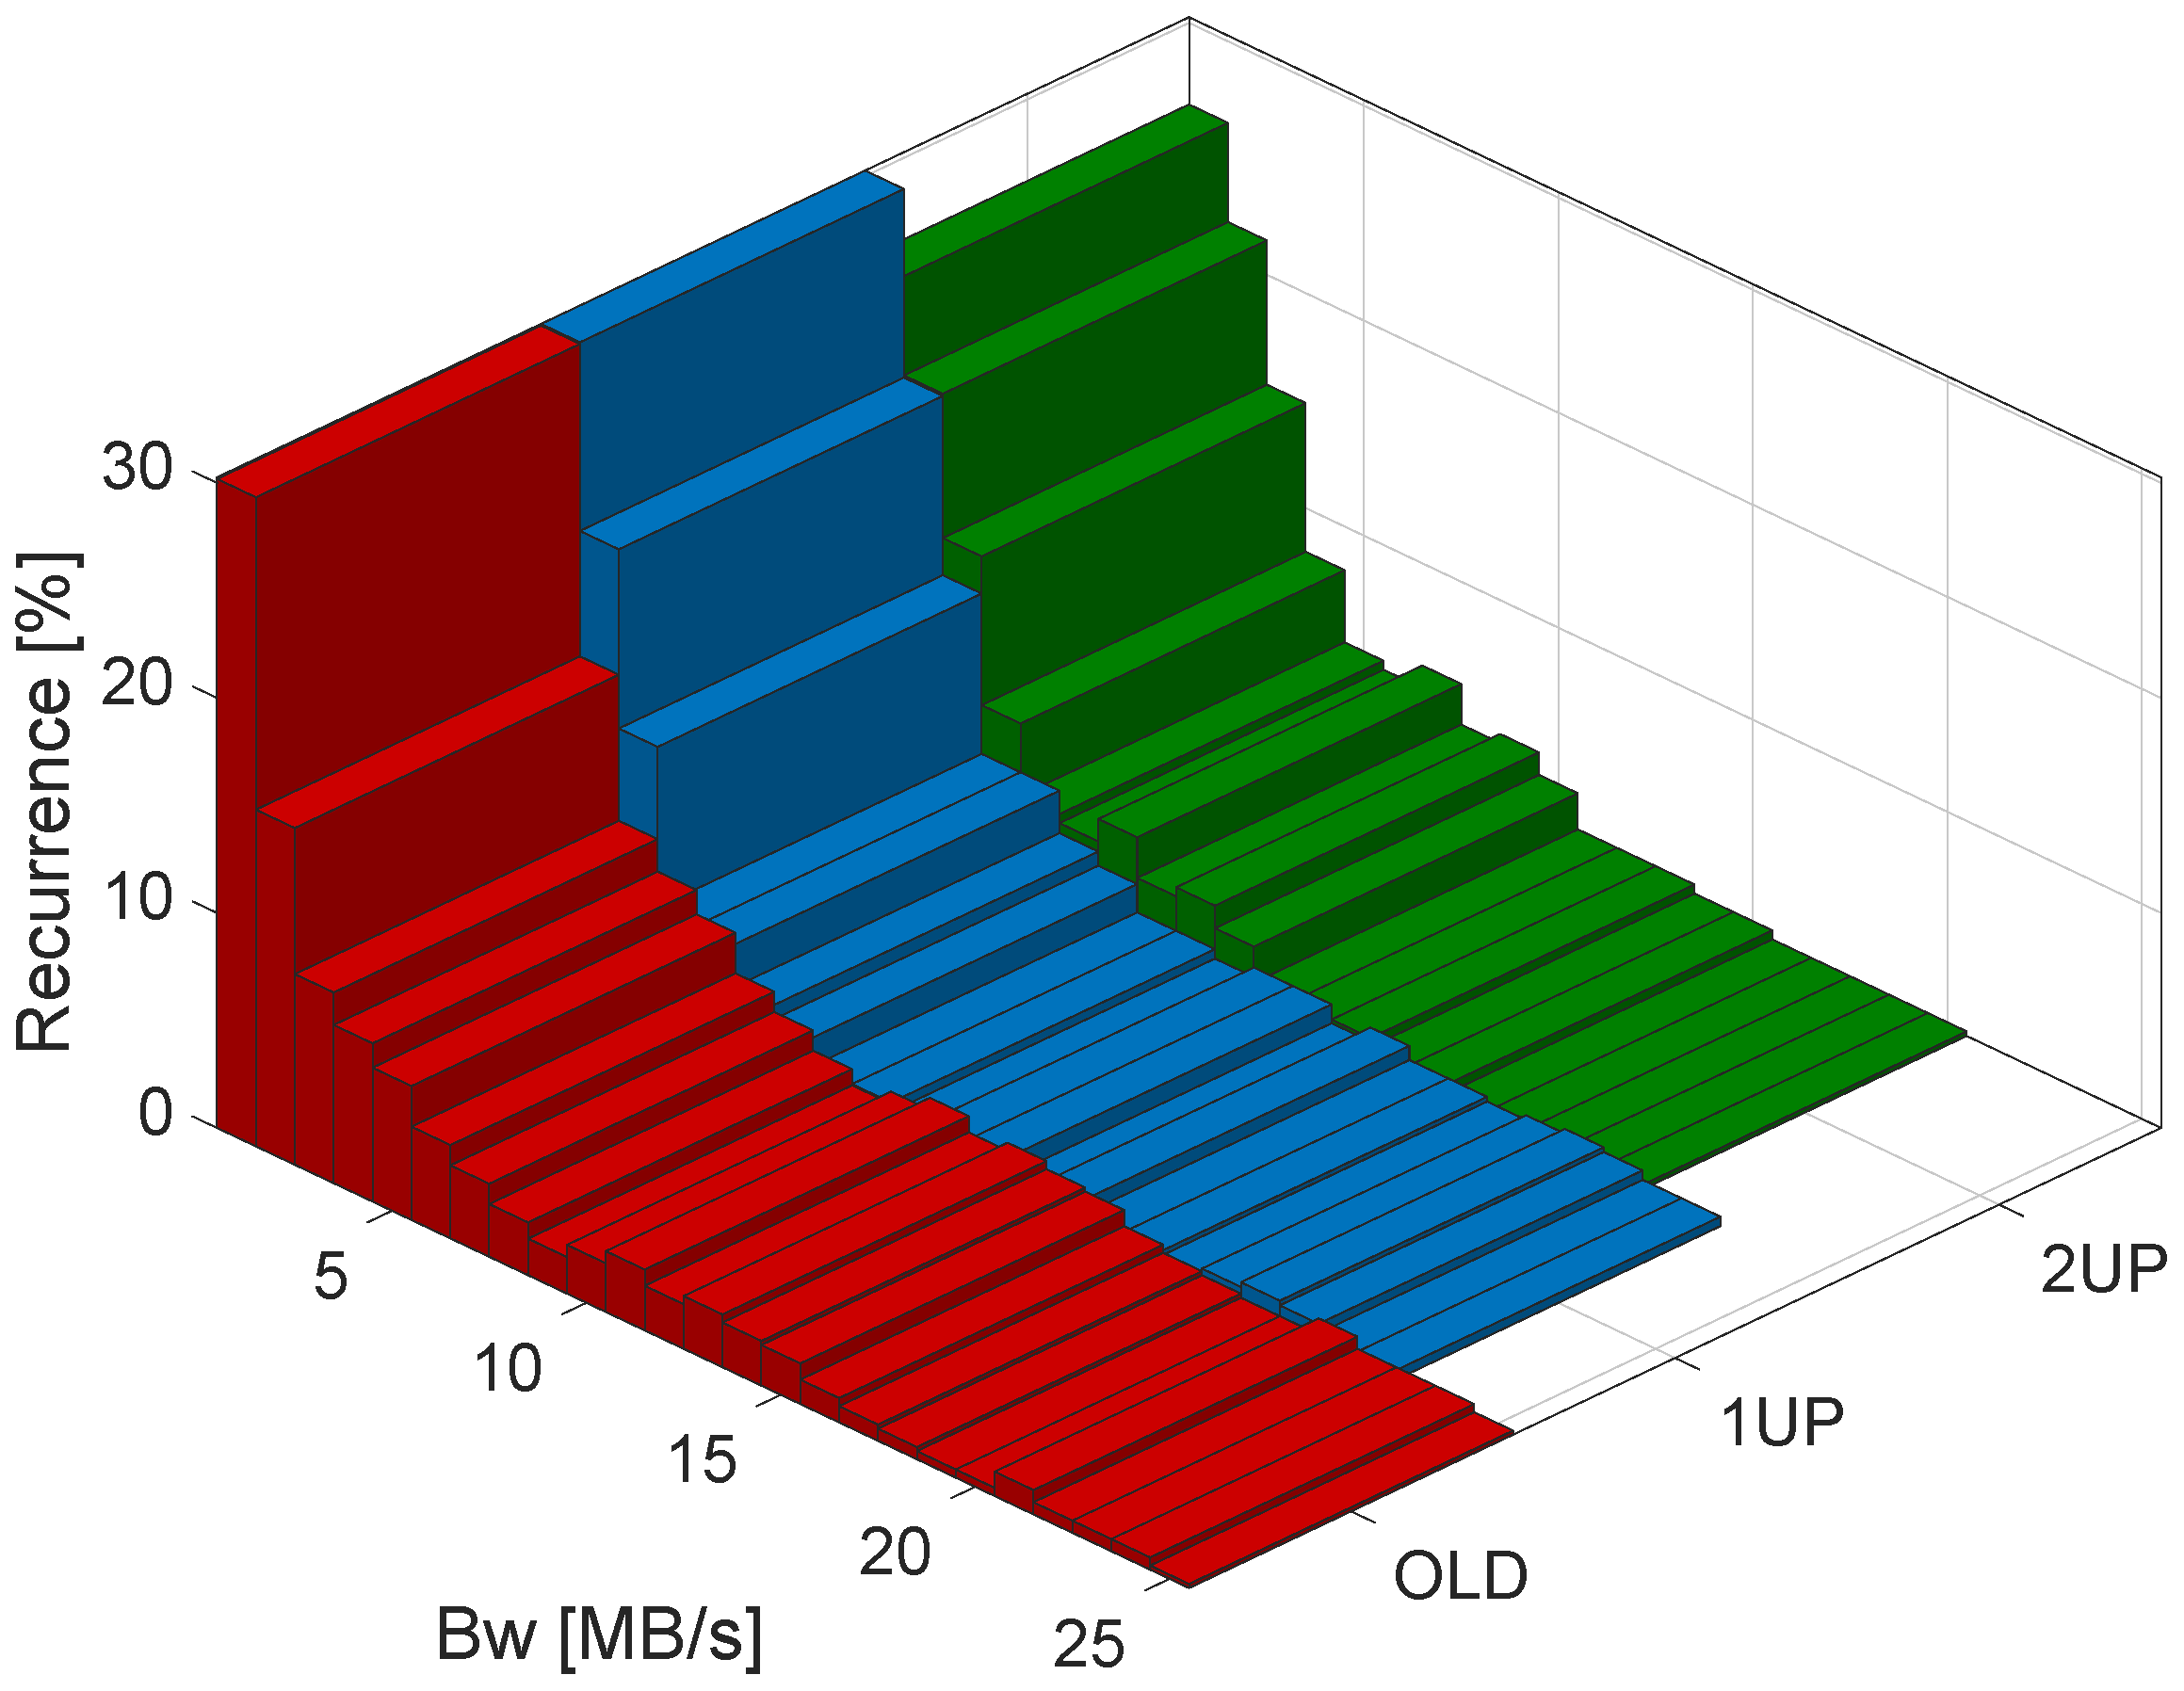
\includegraphics[width=0.7\linewidth]{figure/BW_NoPred.eps}}
\subfigure[b][]{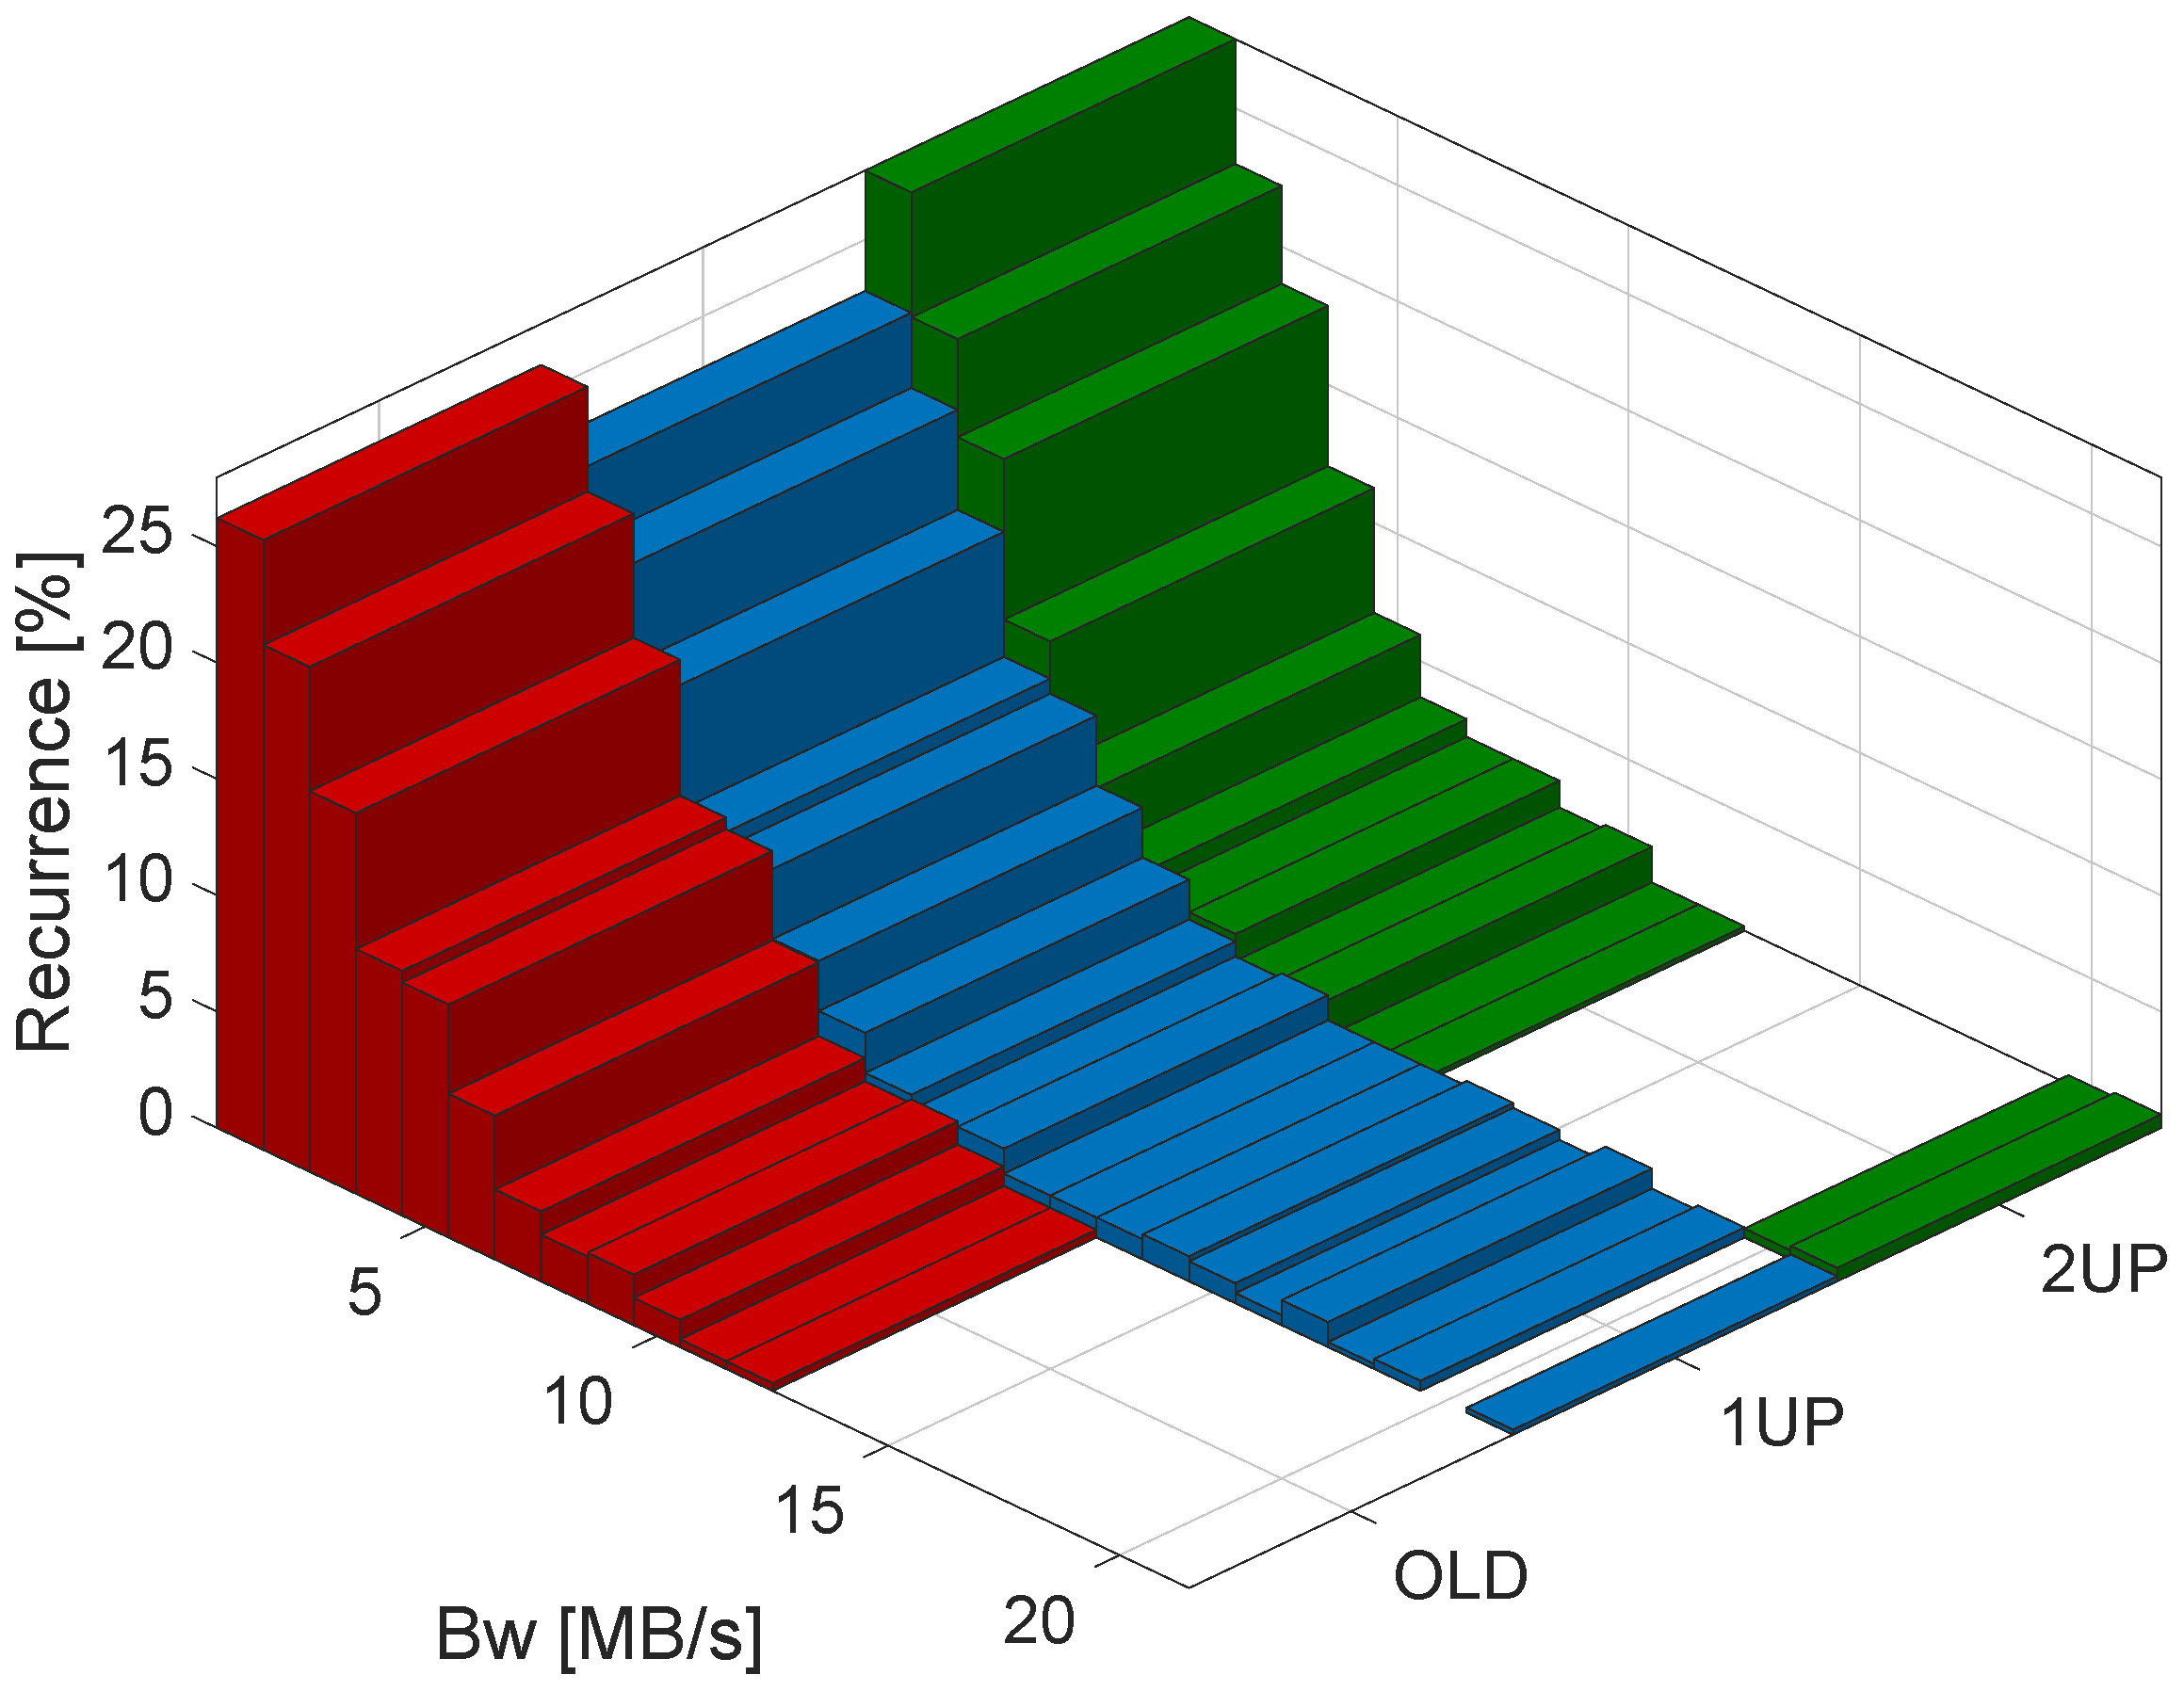
\includegraphics[width=0.7\linewidth]{figure/BW_Pred.eps}}
\caption{Bandwidth saving comparison without (a) and with (b) prediction of the future disturbances.}
\label{fig:BW}
\end{figure}

Figure \ref{fig:BW} illustrates the bandwidth savings showing the recurrence of the different bandwidth usage during the simulations, respectively without and with prediction of the future disturbances. Without disturbance forecast it is exploited up to $25MB/s$ using the OLD model, while it is exploited at most $22MB/s$ and $21MB/s$ respectively for models 1UP and 2UP. Using disturbance forecast, as expected, even less bandwidth is exploited.

\begin{figure}[h!]
\centering
\includegraphics[trim={120 0 120 0},width=0.9\linewidth]{figure/MPCfinal.eps}
\caption{Static controller up to the $400th$ sample, then MPC controller.}
\label{fig:{MPC}}
\end{figure}
\begin{figure}[h!]
	\centering
	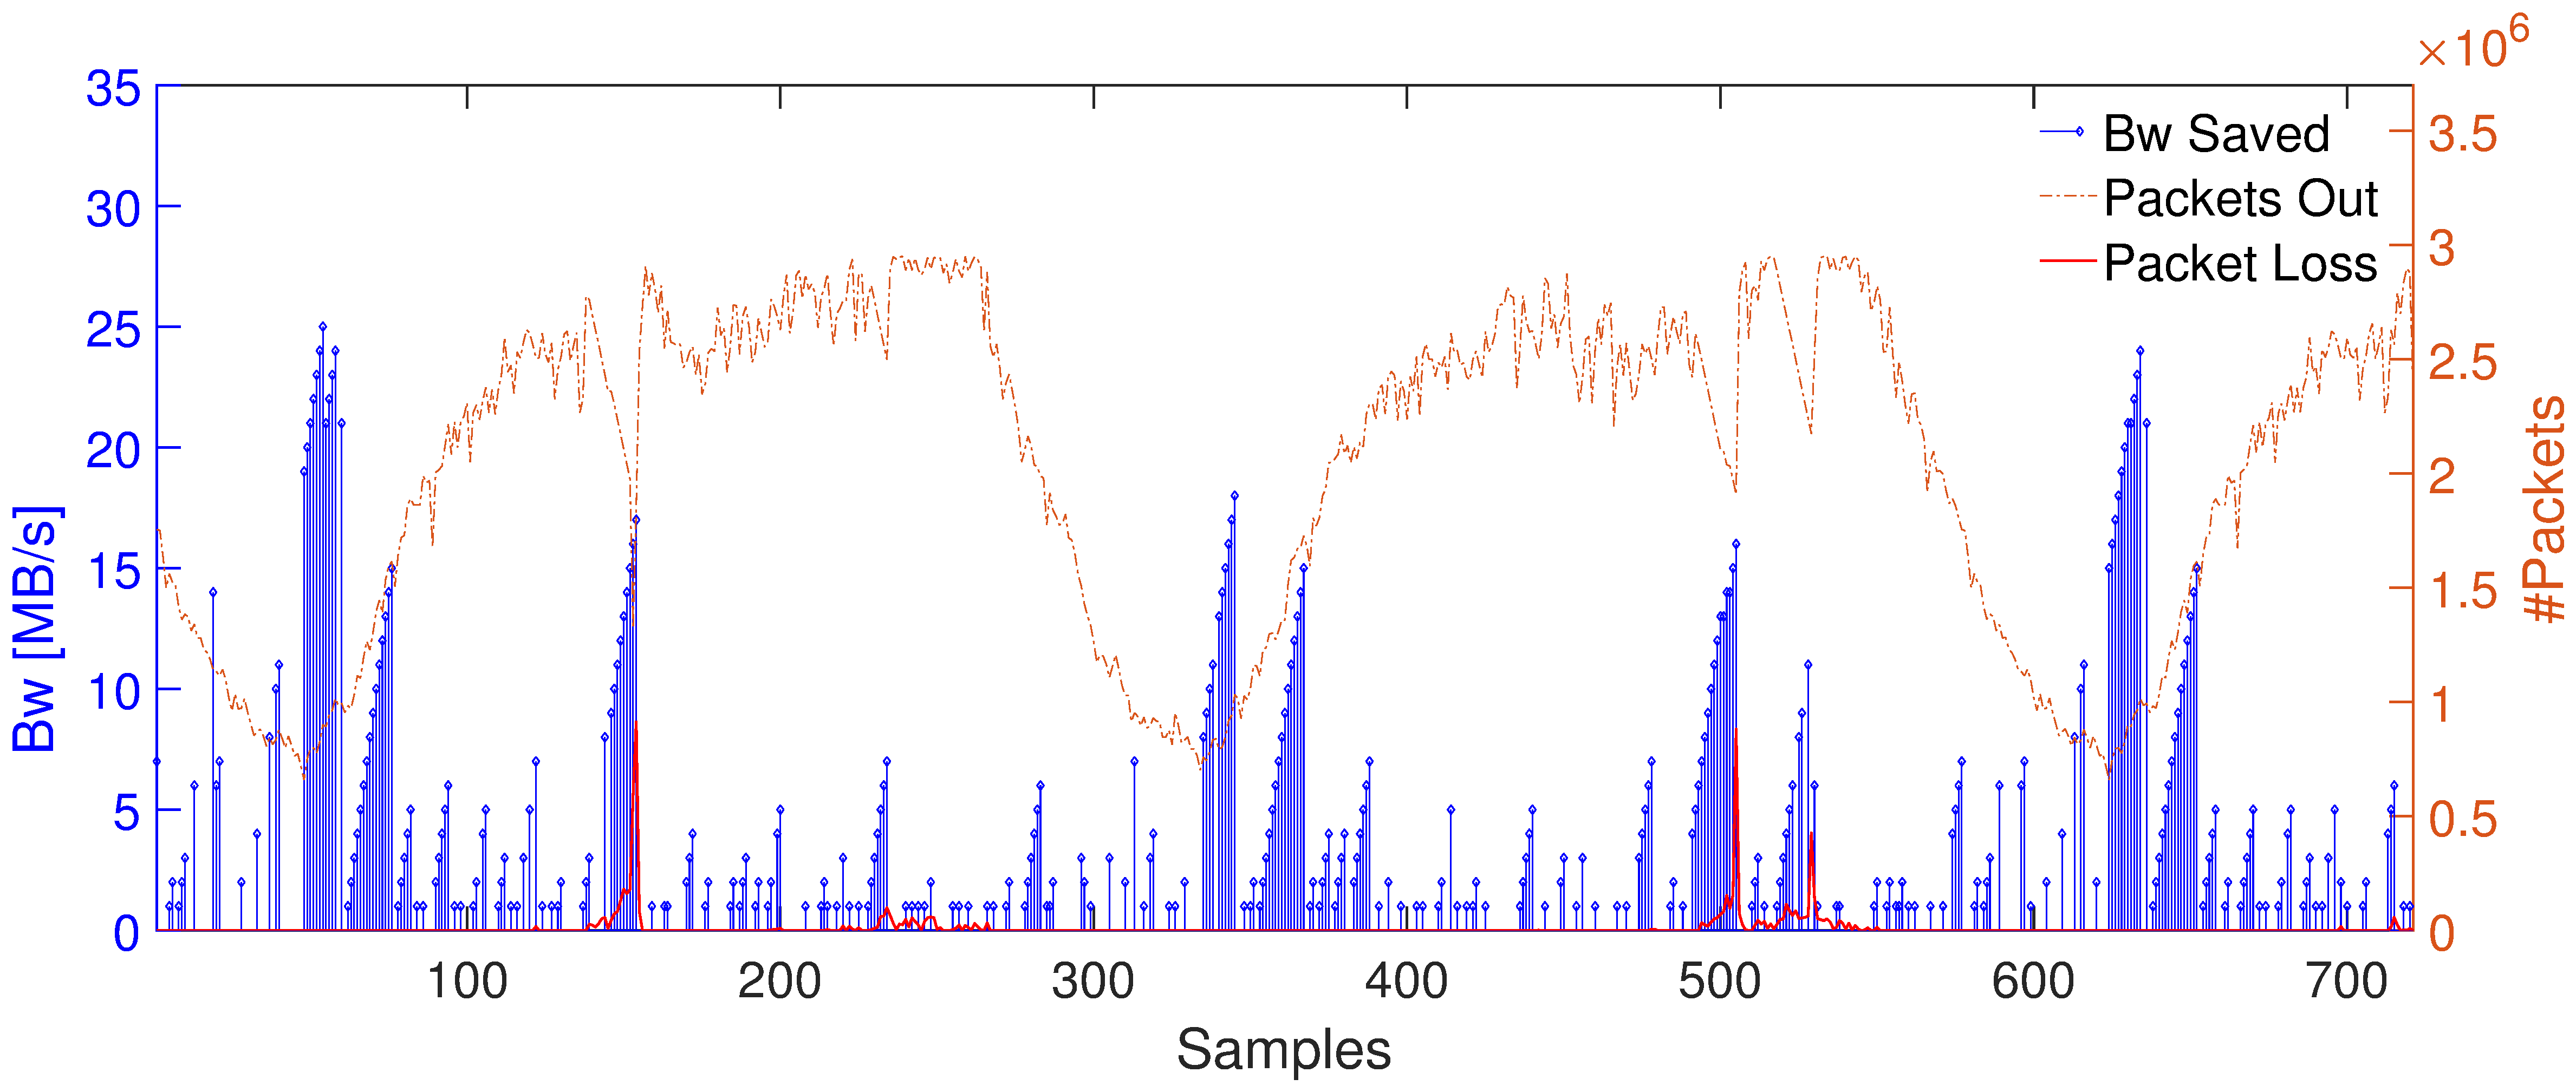
\includegraphics[trim={120 0 120 0},width=1\linewidth]{figure/Banda.eps}
	\vspace{-0.2cm}
	\caption{MPC controller: packets sent from the queues (orange), packets lost (red), bandwidth saving (blue).}
	\vspace{-0.5cm}
	\label{fig:{BWsave}}
\end{figure}


In conclusion to this section, it will be shown the gap between priority queueing control performance of MPC, obtained solving Problem \ref{pbMPC} and based on the proposed RF predictive model, with the static control policy adopted by service provider networks in \cite{Notiziario}. Figure \ref{fig:{MPC}} highlights the dramatic improvement of MPC with respect to static control: the red line shows the incoming traffic, the blue line shows the sum of the packets sent from the queues, and their difference represents packet losses. Until the $400th$ sample static control has been implemented as in \cite{Notiziario}, generating many packet losses due to queues saturation. From that sample to the end of the experimentation MPC is implemented using RF-based model, and the packet loss is drastically reduced: quantitatively, after $700$ sampling periods the cumulative number of dropped packets with the static policy is about $5.5\cdot10^8$ versus $6.6\cdot10^6$ with MPC, with a decrease of $5.434\cdot10^8$ lost packets ($-88 \%$).
%Figure \ref{fig:{BWsave}} shows the amount of bandwidth that our method leaves unused at each time sample (blue line): during the simulation period we were able to save an average $3 MB/s$ with respect to static control, with peaks of more than $20 MB/s$, that can be of course allocated to improve the quality of other services.
Even thought the improvement of MPC with respect to static control is not surprising, much better performance can be obtained in real networks just collecting historical data and applying a controller that can be directly implemented using the accurate models of the proposed identification algorithms and Quadratic Programming standard solvers.

%====================================================================================================
%====================================================================================================
%\chapter{Metrics Evaluation and Estimations}\label{chap4}  % chapter 4
%
This chapter presents the activities related to the evaluation/estimation of metrics useful to extract as-much-as-possible information about system features (e.g., execution time, power/energy consumption, processes interaction and communication). These metrics will be used into the DSE activity (described in Chapter~\ref{dse_chapter_ref}) in order to find HW/SW feasible solutions w.r.t. input NFR.\blfootnote{As reported in the Introduction, this Chapter is related to the following author's contribution: \#4} 
%
\section{Affinity}\label{aff_section}
%
The first metric considered in this Thesis is the \textbf{Affinity} \cite{bib27,affinity_001}. This metric indicates the most suitable PU elements from the proposed BBs for the execution of a given functionality (i.e., blocks of statements), as presented in Definition~\ref{index_01_affinity}. As presented in \cite{bib27,affinity_001}, a possible Affinity measurement activity can be related to the static detection of the most suitable PU classes (e.g., GPP, ASP, SPP). For this, an architectural analysis of this PU classes has been proposed in order to determine their relevant features. Finally, a set of metrics able to provide indications to drive designer choices through the definition of a set of specification patterns has been produced in output. \par
In particular, the Affinity \cite{bib27,affinity_001} of a method $m$ can be expressed by the following function:
%
\begin{equation} \label{equation_affinity}
  \begin{aligned}
    A^T_m = f(W \cdot C^T_m)
\end{aligned}
\end{equation}
%
where
%
\begin{equation} \label{equation_affinity}
\centering
  \begin{aligned}
    A_m &= [A_{{GPP}_m} \ A_{{ASP}_m} \ A_{{SPP}_m}], \\ \\
    W &= 
    \begin{bmatrix} 
        0 & 0 & 0 & 0 & 0 & 0 & 1 & 1 & 0 & 0 & 0 & 1 & 1 & 1 \\
        1 & 1 & 1 & 1 & 1 & 1 & 0 & 0 & 1 & 0 & 0 & 0 & 1 & 0 \\
        0 & 0 & 0 & 0 & 0 & 0 & 0 & 0 & 1 & 1 & 1 & 0 & 0 & 0 
    \end{bmatrix}, \\ \\
    C_m &= [SCD_m, WCD_m, SHD_m, WHD_m, SMD_m, WMD_m, IOR_m, \\
    & \ \ \ \ \ CR_m, LR_m, BMR_m, DR^m_{bit}, \displaystyle \sum_{z \in {int,read}} DR^m_z,STR_m] \\ \\
    f(x) &= \frac{\arctan 2 \pi x^2}{\pi / 2}
\end{aligned}
\end{equation}
%
%An extension of this metric was proposed in \cite{affinity_002_new}, where the Affinity metric has been enriched with a parallelism metric. 
%
\section{Concurrency (Parallelism)}\label{comm_con_metric_eval}
%
This section presents the metrics related to processes and channels behavior characteristics (in terms of concurrency). More specifically, their evaluation relies on the use of the HEPSYCODE Simulator (HEPSIM) software, where the concurrency has been calculated counting all active processes and channels pairs every times a communication occurs (more details in Section~\ref{concurrency_explain}). 
%There is an event (boolean) array in the CSP channel implementation, that represents processes and channel states (1: waiting, 0: idle or stopped). Each times a process or a channel is ready, the corresponding value in the concurrency matrices is increased (every times a communication happens). 
These values are stored in a proper matrix and then normalized to the maximum values that arises from the sum of each column value in the corresponding of every single row in the matrix. The first output of this activity is the so called \textit{Processes Concurrency Matrix}:
%
\begin{equation} \label{eq4}
\small
\begin{aligned}
	{PCON}=\ \left[  
	\begin{array}{cccc}
	{pcon}_{1,1} & {pcon}_{1,2} & \cdots  & {pcon}_{1,n} \\ 
	{pcon}_{2,1} & {pcon}_{2,2} & \cdots  & {pcon}_{2,n} \\ 
	\vdots      & \vdots      & \vdots  & \vdots  \\ 
	{pcon}_{n,1} & {pcon}_{n,2} & \cdots  & {pcon}_{n,n} 
	\end{array}
    \right]   \\ 
\end{aligned}
\end{equation}
%
$PCON$ provides information about how much the processes pairs can be concurrently ``working'', where $PCON = \{ \ pcon_{i,j} \neq 0 \ : \ ps_{i} \land ps_{j}$ can be potentially executed concurrently$\} \in \mathbb{R}^{n \times n}$. \par
The second output of this activity is the \textit{Channels Concurrency Matrix}:
%
\begin{equation} \label{eq4_ch}
\small
\begin{aligned}
	{CCON}=\ \left[  
	\begin{array}{cccc}
	{ccon}_{1,1} & {ccon}_{1,2} & \cdots  & {ccon}_{1,c} \\ 
	{ccon}_{2,1} & {ccon}_{2,2} & \cdots  & {ccon}_{2,c} \\ 
	\vdots      & \vdots      & \vdots  & \vdots  \\ 
	{ccon}_{c,1} & {ccon}_{c,2} & \cdots  & {ccon}_{c,c} 
	\end{array}
    \right]   \\ 
\end{aligned}
\end{equation}
%
$CCON$ provides information about how much the channel pairs can be concurrently transmitting data, where $CCON = \{ \ ccon_{i,j} \neq 0 \ : \ ch_{i} \land ch_{j}$ can be potentially exchange data concurrently$\} \in \mathbb{R}^{c \times c}$. \par
%
\section{Communication}\label{comm_con_metric_eval_only_comm}
%
The communication metric is the sum of the size, in bit, of each data exchanged between each process pairs, and the \textit{Communication Matrix} has been produced as output of this step:
%
\begin{equation} \label{eq8}
\small
\begin{aligned}
{CM}=\ \left[  
\begin{array}{cccc}
{cm}_{1,1} & {cm}_{1,2} & \cdots  & {cm}_{1,n} \\ 
{cm}_{2,1} & {cm}_{2,2} & \cdots  & {cm}_{2,n} \\ 
\vdots      & \vdots      & \vdots  & \vdots  \\ 
{cm}_{n,1} & {cm}_{n,2} & \cdots  & {cm}_{n,n} 
\end{array}
\right]   \\ 
\end{aligned}
\end{equation}
%
$CM$ is expressed by the number of bits sent/received over each channel, where $CM = \{ \ cm_{i,j} \neq 0 \ : \ ps_{i} \land ps_{j}$ exchange $cm_{i,j}$ total amount of data between them$\} \in \mathbb{R}^{n \times n}$. 
%
\section{Timing}\label{timing_metric_def}
%
The goals of this Section are to analyze the usefulness and the meaningfulness of a metric that is concurrently “Off the Shelf”, “HW/SW Unifying”, and “Statement Level”. In fact, to overcome existing metrics limitations \cite{bib25}, the idea is to consider one related to \textbf{Clock Cycles for C Statement} (CC4CS), i.e., the number of clock cycles needed to a specific processor technology to execute a \textit{common C statement}. So, it is at statement-level of abstraction and, thanks to even more improved \textit{High-Level Synthesis} (HLS) tools that are able to synthesize C functions, it is targeted to both SW and HW processor technologies (i.e., \textit{HW/SW unifying}): processors built to execute a given ISA (\textit{General Purpose Processors}, GPP; \textit{Application Specific Processors}, ASP) and processors built to directly (i.e., NO ISA involved) execute applicative functions (\textit{Single/Specific Purpose Processors}, SPP). So, such a metric would be an ideal one for the very early steps of an ESL HW/SW Co-Design Methodology but also for the comparison of SW implementation performances. 
%However, some critical issues soon arise when thinking with more attention to CC4CS. First of all, the concept of \textit{generic C statement} is ambiguous, since a C statement is not a-priori limited in complexity and can give rise to very different HW/SW implementations. Second, to evaluate it in a standard, repeatable, fast and low-cost way, they are needed an evaluation framework and a meaningful set of benchmark functions. The first point can be addressed by considering as “generic C statements” the most common way a programmer writes them (so it is better to talk about \textit{common C statements}), and this consideration should drive the selection of the adopted benchmark. An encouraging precedent can be considered the work done for the definition of the very first (and successful) COCOMO model \cite{cocomo} where, by analyzing a very huge set of source codes, a relationship by the number of \textit{Lines of Code} (LOC) and the SW development cost has been identified, independently by the complexity of each line. The second point, other than identifying a relevant benchmark, can be addressed by designing a proper framework for CC4CS evaluation. 
%So, this work mainly focuses on the development of such a framework and, by means of a simple benchmark, tries to evaluate usefulness and meaningfulness of CC4CS to understand if further effort must be invested in such a direction.
%
\subsection{Definition of CC4CS: an Off-the-Shelf Unifying Statement Level Performance Metric for HW/SW Technologies}
%
The proposed metric is related to C programming language statements, so it is called CC4CS (\textit{Clock Cycles for C Statement}). The choice of the C language is motivated by the following three reasons: it is the most used language for embedded SW development; it is very similar to \textit{SystemC} \cite{bib24_a} (especially when focusing on \textit{SystemC Synthesizable Subset}), one of the most used specification languages for HW/SW co-design; the most diffused HLS (\textit{High Level Synthesis}) tools are able to realize SPPs that implements an algorithm specified in C/SystemC language. 
%
\theoremstyle{definition}
\begin{definition}{(\textit{Clock Cycles For C Statements}).}\label{def1_1}
For a given processor X, CC4CS(X) is the number of clock cycles needed by processor X to execute a common C statement
\end{definition}
%
A first clarification is due with respect to the concept of “common C statement”. It could be generally intended as “something that ends with a semicolon” (other views are possible too, e.g., Table 6.1 in \cite{bibCC4CS02}) but, to avoid ambiguity, this work adopts an empirical approach: it refers to the way a common profiling tool as gcov \cite{bibCC4CS03} performs the C statements identification when profiling their execution. Another clarification is related to the fact that such a metric will be for sure influenced by the used compiler or HLS tool. Some ways to manage this issue could be: to specify also the used tools (possibly giving rise to a set of CC4CS for each processor); to report the average of the results obtained by using the most diffused tools; to report only the results related to the most diffused one. At this point, it is quite clear that CC4CS, as defined above, will be influenced by several factors and that a CC4CS-based estimation will be affected by relevant errors. However, these are acceptable by keeping in mind the following aspects: it is a straightforward way to have an off-the-shelf metric; it can be applied to each processor technology (i.e., GPP, ASP and SPP); it is intended to be used for very early performance analysis in SW and HW/SW domains. Anyway, CC4CS can be also characterized by a set of values related to \textit{Min}, \textit{Max}, \textit{Average}, and \textit{Standard Deviation} (or by a statistical distribution). In this way, it is possible to perform different analysis depending on the final goal.
%
%
\subsection{Timing estimation activity in HEPSYCODE framework}\label{exploit_CC4CS_01}
%
As said before, the CC4CS metric is used to estimate the execution time of different processes on different PU technologies. This is used as an alternative to the standard Cycles Per Instruction (CPI) or Million Instructions Per Second (MIPS) values, and another advantage of this metric is the fact that it is not a single value but a distribution. To exploit such a feature, the affinity metric is used to assign a fixed (singular) CC4CS value to the execution of each process statements (it is also possible to select the min, average, maximum, median values as an alternative, to perform different kind of analysis), using a linear interpolation to evaluate CC4CS value for each function Affinity. \par
%
\begin{figure}[htbp!]
	\centerline{\includegraphics[width=0.7\linewidth]{img/boxdiagram_LEON3_int8.png}}
	\caption{CC4CS distribution for LEON3 int8 data type benchmark.}
	\label{boxplot_cc4cs_show}
\end{figure} 
%
As an example, it is possible to consider the CC4CS distribution shown in Figure~\ref{boxplot_cc4cs_show}. From this box plot and distribution is difficult to chose a fixed CC4CS value without any knowledge of the input application behaviour. It is possible to chose the median value, the second or third quartile and so on. In order to help this "decision" step, Figure~\ref{boxplot_cc4cs_show_solution} propose a mixed approach combining Timing and Affinity metrics (defined in Section~\ref{aff_section}). In such a scenario, it is possible to choice the CC4CS value with the equations shown in Figure~\ref{boxplot_cc4cs_show_solution}, w.r.t. a \textit{Best Case} (Affinity, median, first quartile and third quartile have been considered), an \textit{Average Case} (Affinity, median and the interquartile range, IRQ, have been considered), or a \textit{Worst Case} (Affintiy, median, min and max distribution values have been considered).
%
\begin{figure}[htbp!]
	\centerline{\includegraphics[width=0.9\linewidth]{img/CC4CS_affinity.png}}
	\caption{CC4CS timing metric assignment with Affinity value.}
	\label{boxplot_cc4cs_show_solution}
\end{figure} 
%
\begin{comment}
%
\section{Bandwidth}
%
The bandwidth estimation considers each communication operation, evaluating the size of exchanged data in the following equation:
%
\begin{equation} \label{eq20_ch_bandwidth}
\resizebox{0.6 \textwidth}{!}{$%
\begin{aligned} 
    BW = (\# data \ exchanged \ \ [bits]) * (link \ speed \ \ [bits/s])
\end{aligned}
$%
}
\end{equation}
%
\end{comment}
%
\section{Load}\label{load_metric}
%
Finally, the Load metric is related to the execution of processes on a single instance of PU. In particular, by allocating all the \textit{n} processes to a single instance of each SW processor $pu_{k}$ and performing a timing simulation for each one,  three parameters are computed: 
%
\begin{itemize}
    \item \textit{$FRT_{k}$ (Free Running Time)}, i.e., the total simulated time on processor $pu_{k}$;
    \item \textit{$t_{k,j}$}, the simulated time for each process \textit{$ps_{j}$} on processor \textit{$pu_{k}$};
    \item \textit{$N_{k,j}$,} the number of executions of each process \textit{$ps_{j}$} on processor \textit{$pu_{k}$} (i.e., the number of loops).
\end{itemize}
%
Starting from these parameters, it is possible to define the \textit{Free Running Load Matrix} \textit{$FRL$}:
%
\begin{equation} \label{eq12}
\small
\begin{aligned}
{FRL} = \left[  
\begin{array}{cccccc}
{frl}_{1,1} & {frl}_{1,2} & \cdots  & {frl}_{1,j} & \cdots & {frl}_{1,n} \\ 
{frl}_{2,1} & {frl}_{2,2} & \cdots  & {frl}_{2,j} & \cdots & {frl}_{2,n} \\ 
\vdots 			& \vdots 		  & \vdots  & \vdots 		  & \vdots & \vdots 		 \\ 
{frl}_{k,1} & {frl}_{k,2} & \cdots  & {frl}_{k,j} & \cdots & {frl}_{k,n} \\
\vdots  		& \vdots 		  & \vdots  & \vdots 		  & \vdots & \vdots 		 \\ 
{frl}_{s,1} & {frl}_{s,2} & \cdots  & {frl}_{s,j} & \cdots & {frl}_{s,n} \\
\end{array}
\right]  \\
where \ {frl}_{k,j} =\frac{\left(t_{k,j} \cdot N_{k,j}\right)}{{FRT}_k} \ \forall  k=1..s, \ j=1..n \ \ \ 
\end{aligned}
\end{equation}
%
where \textit{${FRT}_{k}/N_{k,j}$} is the average period of each processes \textit{$ps_{j}$} on processor \textit{$pu_{k}$}. 
%

%\chapter{Search Methods: The Design Space Exploration Approach} \label{dse_chapter_ref}
%
In the embedded system design domain, the most critical development step is related to the \textit{Design Space Exploration} activities \cite{bib10} and the main differences among the works in the literature are mainly related to the different amount of information and actions that explicitly rely on the designer experience. This section presents mathematical classical models that rely on the definition of multi-criterion optimization problems and presents the injection of mixed-criticality requirements into the classical representation one.\blfootnote{As reported in the Introduction, this Chapter is related to the following author's contribution: \#2, \#3, \#4} 
%
\section{The Single-Objective Optimization Problem}
Considering engineering area, mathematical description of single-objective problems related to minimize or maximize a single objective function $f(\bar x)$ over a set of decision variables $\bar x$ limited by constraints functions has been widely treated in literature. Generally, a single-objective optimization problems (SOOPs) can be defined as \cite{bib1Chiandussi}:
\theoremstyle{definition}
\begin{definition}{(\textit{General Single-Objective Optimization Problem}).} Given a function $ f : \Omega \subseteq \mathbb{R}^{n} \to \mathbb{R}, \Omega \not= 0$, a general single-objective optimization problem is defined as: 
%
\begin{equation} \label{equation111}
  \begin{aligned}
    & \underset{\bar x}{\text{min}} &  & f(\bar x) \\
    & \text{subject to}             &  & \bar x \in \Omega
\end{aligned}
\end{equation}
%
where $\bar x$ is a n-dimensional decision variable vector, $\bar x = \{x_1,\ldots, x_n\}$ and $\Omega$ is the computation variable space normally described by function constraints (continuous or discrete) which limit $f$ objective function (and indirectly $\bar x$).
\end{definition}
%
Finding a global optimum of any function (that could not be unique) is known as Global Optimization problem. In general, the goal to determining the global minimum solution of a single-objective problem is defined as \cite{bib2}:
%
\theoremstyle{definition}
\begin{definition}{(\textit{Single-Objective Global Minimum Optimization}).}\label{def1}
Given a function $ f : \Omega \subseteq \mathbb{R}^{n} \to \mathbb{R}, \Omega \not= 0$, for $\bar x \in \Omega$ the value $f^\ast \triangleq f(\bar x^\ast) > -\infty$ is called a global minimum if and only if: 
%
\begin{equation}\label{equation112}
  \begin{aligned}
    & \forall \bar x \in \Omega : f(\bar x^\ast) \leq f(\bar x)
\end{aligned}
\end{equation}
where $\bar x^\ast$ is the global minimum solution, $f$ is the objective function and $\Omega$ is the feasible region of $\bar x$.
\end{definition}
%
\section{The Multi-Objective Optimization Problem}
Usually, in optimization problems, there is more than one objective function that can be considered (i.e., minimize cost, power consumption, maximize performance, througput etc.), but most of the time objectives are often conflicting. This kind of optimization issues are called "Multi-objective optimization problems" (MOOP), where multiple objectives have to be optimized simultaneously. Typically, a MOOP can be defined as follows \cite{bib3}:
%
\theoremstyle{definition}
\begin{definition}{(\textit{General Multi-Objective Optimization Problem}).}
Given a function $ \bar F : \Omega \subseteq \mathbb{R}^{n} \to \mathbb{R}^k, \Omega \not= 0$, a general multi-objective optimization problem is defined as:
%
\begin{equation}\label{equation113}
  \begin{aligned}
    & \underset{\bar x}{\text{min}} &  & \bar F(\bar x) = [f_1(\bar x), f_2(\bar x), \ldots , f_k(\bar x)] \\
    & \text{subject to}             &  & \bar x \in \Omega
\end{aligned}
\end{equation}
%
where $\bar x = \{x_1,\ldots, x_n\}$ is an n-dimensional decision variable vector in the solution space $\Omega$ (which refers to a feasible search space, feasible set of decision vectors) and $\mathbb{R}^k$ refers to the objective space. $\bar F(\bar x) = [f_1(\bar x), f_2(\bar x), \ldots , f_k(\bar x)] \in \mathbb{R}^k$ consists of k $\geq 2$ real value objective functions. The solution space $\Omega$ is generally restricted by a series of constraints and bounds on the decision variables.
%
\end{definition}
%
Given $\bar x \in \Omega$, find a vector $\bar x^\ast$ that minimizes k objective functions $\bar F(\bar x) = [f_1(\bar x), f_2(\bar x), \ldots , f_k(\bar x)] \in \mathbb{R}^k$ is not simple because optimizing $\bar x$ (with respect to a single objective) often results unacceptable with respect to other objectives. Therefore, a multi-objective solution that simultaneously optimizes each objective function is almost impossible, so a solution to a multi-objective problem is to find a set of solutions, each of which satisfies the objectives without being dominated by any other solution (the concept of domination will be introduced later). \par
%
\begin{figure}[htbp]
	\centerline{\includegraphics[width=1.0\linewidth]{img/00-Multi-objective-optimization-problems.png}}
	\caption{Mapping of a multi-objective problem.}
	\label{fig_multiobjmapp}
\end{figure}
%
Since SOOPs may have a unique optimal solution, MOOP present a possibly infinite set of solutions. Two $\mathbb{R}$ Euclidean spaces are considered in multi-objective problems, as shown in Fig.~\ref{fig_multiobjmapp}:
%
\begin{itemize}
    \item  the n-dimensional decision variables space ($\mathbb{R}^n$) in which each axis corresponds to an element of vector $\bar x$;
    \item the k-dimensional objective functions space ($\mathbb{R}^k$) in which each axis corresponds to the element vector $f_k(\bar x)$.
\end{itemize}
%
The function $ \bar F : \Omega \subseteq \mathbb{R}^{n} \to \mathbb{R}^k$, maps the decision variables vector $\bar x = \{x_1,\ldots, x_n\} \in \mathbb{R}^n$ to vectors $\bar F = \{f_1,\ldots, f_k\} \in \mathbb{R}^k$. To find a solution for this kind of problems, Pareto Optimality Theory \cite{bib3} has been defined in research works, in which the optimal solution set is not a single solution but a set of trade-off solutions, namely, Pareto optimal solutions. \par
%
Briefly, in summary, a multi-objective optimization problem (also called multi-criteria optimization problem) can be defined as the problem of \cite{bib5} \textit{''finding a vector of decision variables which satisfies constraints and optimizes a vector function whose elements represent the objective functions. These functions form a mathematical description of performance criteria which are usually in conflict with each other. Hence, the term ‘optimize’ means finding such a solution which would give the values of all the objective functions acceptable to the decision maker''}. \par
Thus, a multi-objective problem consists of k objectives reflected in the k objective functions and n decision variables, where the k objective functions may be linear or nonlinear and continuous or discrete (as the decision variables $x_i$ may be continuous or discrete). During the remainder of this 
work, some basic definition will be presented. \par
%
\section{Basic Definitions}
%
\theoremstyle{definition}
\begin{definition}{(\textit{Convexity}).}\label{defC1}
A function $g(\bar x)$ is called convex over the domain of $\mathbb{R}$ if for any two vectors $\bar x_1, \bar x_2 \in \mathbb{R}$:
%
\begin{equation} \label{equation114}
  \begin{aligned}
    g(\alpha \bar x_1 + (1 - \alpha)\bar x_2) \leq \alpha g(\bar x_1) + (1-\alpha)g(\bar x_2), \ \ 0 \leq \alpha \leq 1
\end{aligned}
\end{equation}
%
\end{definition}
It should be noted that $g(\bar x)$ is concave if $-g(\bar x)$ is convex.
%
\theoremstyle{definition}
\begin{definition}{(\textit{Convex Set}).}\label{defC1C2}
A set of points (or a region) is defined as a convex set $\Omega$ in n-dimensional space if:
%
\begin{equation} \label{equation115}
  \begin{aligned}
    \forall x_1, x_2 \in \Omega, \ \bar x = \alpha \bar x_1 + (1-\alpha)\bar x_2 \in \Omega, \ \ 0 \leq \alpha \leq 1  
\end{aligned}
\end{equation}
%
\end{definition}
Fig.~\ref{fig_convex} shows few examples of convex sets, and Fig.~\ref{fig_concave} shows few examples of non-convex sets.
%
\begin{figure}[htbp]
	\centerline{\includegraphics[width=0.8\linewidth]{img/convex.png}}
	\caption{Convex Sets.}
	\label{fig_convex}
\end{figure}
%
\begin{figure}[htbp]
	\centerline{\includegraphics[width=0.8\linewidth]{img/convexNO.png}}
	\caption{Non-Convex Sets.}
	\label{fig_concave}
\end{figure}
%
\theoremstyle{definition}
\begin{definition}{(\textit{Pareto Dominance}).}\label{defC2}
A vector $\bar u = (\bar u_1, \ldots , \bar u_k)$ is said to dominate another vector $\bar v = (\bar v_1, \ldots , \bar v_k)$ (denoted by $\bar u \preceq \bar v$) if and only if $\bar u$ is partially less than $\bar v$:
%
\begin{equation} \label{equation116}
  \begin{aligned}
    \forall i \in \{ 1, \ldots , k\}, \ u_i \leq v_i \ \wedge \ \exists i \in \{1, \ldots , k\} :  u_i < v_i
\end{aligned}
\end{equation}
%
\end{definition}
%
\theoremstyle{definition}
\begin{definition}{(\textit{Pareto Optimality}).}\label{defC3}
A solution $\bar x^\ast \in \Omega$ is said to be Pareto optimal with respect to $\Omega$ if and only if 
%
\begin{equation} \label{equation117}
  \begin{aligned}
    \nexists  \ \bar x' \in \Omega : \bar v = \bar F(\bar x') = ( f_1(\bar x'), . . . , f_k(\bar x')) \preceq \bar u = \bar F(\bar x^\ast) = ( f_1(\bar x^\ast), . . . , f_k(\bar x^\ast))
\end{aligned}
\end{equation}
%
So, $\bar x^\ast$ is Pareto optimal if there is not feasible vector $\bar x'$ which would decrease/increase some criterion/objective without causing a simultaneous increase/decrease in at least one other criterion/objective assuming minimization/maximization.
%
\end{definition}
%
\theoremstyle{definition}
\begin{definition}{(\textit{Pareto Optimal Set}).}\label{defC4}
For a given multi-objective problem, $\bar F(\bar x)$, the Pareto Optimal Set, $\rho^\ast$, is defined as:
%
\begin{equation} \label{equation118}
  \begin{aligned}
    \rho^\ast = \{ \bar x \in \Omega \ | \ \nexists \ \bar x' \in \Omega : \bar F(\bar x') \preceq \bar F(\bar x)\}
\end{aligned}
\end{equation}
%
\end{definition}
%
\theoremstyle{definition}
\begin{definition}{(\textit{Pareto Front}).}\label{defC5}
For a given multi-objective problem, $\bar F(\bar x)$, and Pareto optimal Set $\rho^\ast$, the Pareto front $\rho F^\ast$ is defined as:
%
\begin{equation} \label{equation119}
  \begin{aligned}
    \rho F^\ast = \{ \bar u = \bar F(\bar x) \ | \ \bar x \in \rho^\ast\}
\end{aligned}
\end{equation}
%
\end{definition}
%
The standard procedure to generate the Pareto front is to compute many points in $\Omega$ and their corresponding objective images. Whit a sufficient number of points, it is possible to find the non dominated vector set and the relative Pareto front. A sample Pareto Optimal Set and Pareto Front are shown in Fig.~\ref{fig_paretofront}.
%
\begin{figure}[htbp]
	\centerline{\includegraphics[width=0.9\linewidth]{img/paretoFront.png}}
	\caption{Example of Pareto Front and Pareto Optimal set.}
	\label{fig_paretofront}
\end{figure}
%
\theoremstyle{definition}
\begin{definition}{(\textit{Ideal Point}).}\label{defC6}
The ideal point $\bar F^I = \{ f^I_1, \ldots , f^I_k\}$ is the vector composed with the best objective values over the search space. Analytically, the ideal objective vector is expressed by: 
%
\begin{equation} \label{equation120}
  \begin{aligned}
    \bar f^I_i = \underset{\bar x \in \Omega}{\text{min}} \ f_i(\bar x), \ \ i = 1, \ldots , k
\end{aligned}
\end{equation}
%
\end{definition}
%
\theoremstyle{definition}
\begin{definition}{(\textit{Utopian Point}).}\label{defC7}
The utopian point $\bar F^U = \{ f^U_1, \ldots , f^U_k\}$ is the infeasible vector composed with the difference between the components $f^I_i$ of the ideal point and a relative small but computationally significant scalar $\epsilon_i$. Analytically, the ideal objective vector is expressed by: 
%
\begin{equation} \label{equation121}
  \begin{aligned}
    \bar f^U_i = f^I_i - \epsilon_i, \ \ i = 1, \ldots , k
\end{aligned}
\end{equation}
%
\end{definition}
%
\theoremstyle{definition}
\begin{definition}{(\textit{Nadir Point}).}\label{defC8}
The nadir point $\bar F^N = \{ f^N_1, \ldots , f^N_k\}$ is the vector composed with the worst objective values over the Pareto set. Analytically, the nadir objective vector is expressed by: 
%
\begin{equation} \label{equation122}
  \begin{aligned}
    \bar f^N_i = \underset{\bar x \in \Omega}{\text{max}} \ f_i(\bar x), \ \ i = 1, \ldots , k
\end{aligned}
\end{equation}
%
\end{definition}
%
\theoremstyle{definition}
\begin{definition}{(\textit{Weak Pareto Optimality}).}\label{defC9}
A point $\bar x^\ast \in \Omega$ is a weak Pareto optimal if: 
%
\begin{equation} \label{equation123}
  \begin{aligned}
    \nexists \ \bar x \in \Omega : f_i(\bar x) < f_i(\bar x^\ast), \ i = 1, \ldots , k
\end{aligned}
\end{equation}
%
\end{definition}
%
\theoremstyle{definition}
\begin{definition}{(\textit{Strict Pareto Optimality}).}\label{defC10}
A point $\bar x^\ast \in \Omega$ is a strictly Pareto optimal if: 
%
\begin{equation} \label{equation124}
  \begin{aligned}
    \nexists \ \bar x \in \Omega : f_i(\bar x) \leq f_i(\bar x^\ast), \ i = 1, \ldots , k
\end{aligned}
\end{equation}
%
\end{definition}
%
\theoremstyle{definition}
\begin{definition}{(\textit{Multi-Objective Global Minimum}).}\label{defC11}
Given a function $\bar F : \Omega \subseteq \mathbb{R}^n \Rightarrow \mathbb{R}^k, \Omega \not=0, k \geq 2$, for $\bar x \in \Omega$ the set $\rho F^\ast \triangleq \bar f(\bar x^\ast_i) > (-\infty, \ldots, -\infty)$ is called the global minimum if and only if:
%
\begin{equation} \label{equation125}
  \begin{aligned}
    \forall \ \bar x \in \Omega : \bar f(\bar x^\ast_i) \preceq \bar f(\bar x), \ i = 1, \ldots, n
\end{aligned}
\end{equation}
%
$\bar x^\ast_i$ is the global minimum solution set, $\bar f$ is the multiple objective function vector, and $\Omega$ is the feasible region. The problem to find global minimum solution set is called multi-objective global optimization problem \cite{bib1Chiandussi}.
\end{definition}
%
\section{Genetic Algorithm}\label{genetic_algo_section}
%
The concept of Genetic Algorithm (GA) was created by Holland in the 1975 \cite{bibGA}. GA are inspired by Charles Darwin’s theory of natural evolution. In nature, species within their environment are faced with extinction by natural selection and the strongest individual could pass their genes to future children generations via reproduction. In a long period, species succeed to transmit in dominant genes, adapting their condition to the wild environment. Sometimes also random changes may occur in genes and a new species evolve from the old ones. Unsuccessful changes are eliminated by natural selection. \par
In GA terminology, a solution vector $\bar x \in \Omega$ is called an \textit{individual} or a \textit{chromosome} (generally a set of binary digits 0 and 1, but also real or integer values are used). Chromosomes are composed by discrete units called \textit{genes}. Each gene controls one or more characteristic of the chromosome. The values of a gene are known as \textit{alleles} and the set of all genes is called \textit{genotype} of the chromosome. Normally, a chromosome is a unique solution $\bar x$ in the solution space $\Omega$. This requires a mapping mechanism between the solution space and the chromosomes, called \textit{encoding}. The set of encoded real or integer genotypes, called \textit{control factors}, composes the so called \textit{phenotype}. When an objective function is evaluated in correspondence of a chromosome control factors, its value is called \textit{fitness} value of that chromosome, and the function is the \textit{fitness function}. Thus, each chromosome produce a solution to single objective optimization problem. GA operate with a set of chromosomes, called \textit{population}, normally randomly created. Evolving the search method, the population converges to a single solution that dominated any other individuals. \par
%
\begin{algorithm}
    \caption{Classical GA}\label{alg:ga_algorithm1}
    \begin{algorithmic}[1]
        \State Init. Population P
        \Procedure{Evaluation}{$P$}
            \While{Each individual $\bar x$ in population P}
                \State Calculate single objective function $F_i$ for individual $\bar x$ 
                \State Calculate fitness function $F$ for individual $\bar x$
            \EndWhile
            \State Elitism (Optional)
        \EndProcedure
        \State EVALUATION
        \While{!(STOP CRITERIA)}
            \State Selection
            \State Crossover $\land$ Mutation
            \State Survivor Selection
            \Procedure{Evaluation}{$P$}
            \EndProcedure
            \State EVALUATION
        \EndWhile\label{gadwhile}
        \State \textbf{return}
    \end{algorithmic}
\end{algorithm}
%
Algorithm~\ref{alg:ga_algorithm1} shown the classical GA implementation. GA use two steps in order to find new solutions from existing ones: \textit{crossover} and \textit{mutation}. In crossover, generally two chromosomes, called \textit{parents}, are merged together to form two new chromosomes, called \textit{offspring} or \textit{children}. The parents are selected from existing chromosomes in the population respect to the fitness value. Repeating the crossover step for a huge number of iteration, good genes appear more frequently in the population, arriving to the convergence of the final global optimal Pareto solution. The mutation step makes random changes into genes, where the mutation rate is very small and depends on the chromosome size, reintroducing genetic diversity into the population and avoid remaining into local optimal points. It is possible to use \textit{Elitism} to guarantee that solution quality obtained by the GA will not decrease from one generation to the next, copying the best individuals from the current generation to the next one. 
Finally, to select good chromosomes for the next generation, the individual fitness value determines the survival probability. Different selection approaches are presents in literature, as proportional selection, ranking, tournament selection and so on. 
%
%\subsection{Multi-objective Genetic Algorithm: State-of-the-Art}
%
%TODO
%
\subsection{Multi-objective Genetic Algorithm: Fitness Function Assignment}
%
A classical approach to solve a MOOP is the \textit{Weighted Sum Method} (WSM), which assign a weight $\omega_i$ to each objective function $\bar F(\bar x)$ so that the problem is converted to a \textit{Single-Objective Optimization Problem} (SOOP) with a scalar cost function (called \textit{utility function}, defining a relative criterion importance), as follows:
%
\begin{definition}{(\textit{Weight Sum Method}).}
Given a function $ \bar F : \Omega \subseteq \mathbb{R}^{n} \to \mathbb{R}^k, \Omega \not= 0$, a general MOOP can be reduced to a SOOP as defined below:
%
\begin{equation} \label{equation126}
\resizebox{0.7\hsize}{!}{$%
  \begin{aligned}
    & \underset{\bar x}{\text{min}} & & \bar U(\bar x) = \omega_1 \cdot F_1(\bar x) + \ldots + \omega_k \cdot F_k(\bar x) = \sum_{k} \omega_{k} \cdot F_k(\bar x) \\
    & \text{s.t.}             &  & \bar x \in \Omega 
\end{aligned}
$%
}
\end{equation}
%
\end{definition}
Since the magnitude of objective functions could be quite different, a scaling operation can be applied to them \cite{yuea}. In such a case, the final problem definition is as follows:
%
\begin{definition}{(\textit{Scaled Weighted Sum Method}).}
%
The linear combination of WSM can be normalized as defined before:
%
\begin{equation} \label{equation127}
\resizebox{0.7\hsize}{!}{$%
  \begin{aligned}
    & \underset{\bar x}{\text{min}} & & \bar U(\bar x) &= \omega_1 \cdot \frac{F_1(\bar x)}{F^\ast_1(\bar x)} + \ldots + \omega_k \cdot \frac{F_k(\bar x)}{F^\ast_k(\bar x)} &=  \sum_{k} \omega_{k} \cdot \frac{F_k(\bar x)}{F^\ast_k(\bar x)} \\
    & & & &= \omega_1 \cdot F'_1(\bar x) + \ldots + \omega_k \cdot F'_k(\bar x) &= \sum_{k} \omega_{k} \cdot F'_k(\bar x) \\
    & \text{s.t.} &  & \bar x \in \Omega & &
\end{aligned}
$%
}
\end{equation}
%
where $F^\ast_i(\bar x)$ are the scaling parameters for the objective function, so $F'_i(\bar x)$ is the normalized objective function of $F_i(\bar x)$ and $\sum \omega_{i}=1$. 
\end{definition}
%
With this definition, the multi-criteria optimal design problem is changed into a single objective optimal design problem, and can be solved in a relatively straightforward manner, using also genetic algorithm procedure. In fact, it has been demonstrated \cite{miettinen} that (S)WSM provides a sufficient condition for Pareto optimality, and a necessary condition if the decision space $\Omega$ and the feasible criterion space $Z$ are convex. These proprieties are not simple to demonstrates. One methods is to evaluate the Hessian matrix $H(\bar F)$ and to evaluate if it is positive or semi-positive definite, so the considered set are convex. This technique is not simple to be implemented while the input problem depends on application and platform models, so calculating the Hessian matrix value for each input is time consuming. However the non-convexity property relies in a local minimum, and other methods are used in literature (as adaptive weight methods \cite{apost_01}) but it is out of the scope of his work. \par
This approach is called \textit{a priori approach} because decision maker should provide weights in advance. Solving the problem for a fixed weight vector $\bar \omega = \{\omega_1, \omega_2, \ldots , \omega_k \}$ produce a single solution, and the problem must be solved multiple times with different weight combinations if multiple solutions shall be produced, so the selecting of the weight vector for each iteration is a critical point \cite{bibGATutorial}. So the actual problem in the (S)WSM is the required decision maker actions, since it is not easy to consider the overall relative importance of all the cost functions. Moreover, the scaled objective functions can still have different bias in the [0, 1] interval and such an issue should be fixed. So, a method to automatically evaluate weights, but still able to take into account decision maker preferences, is needed. In fact, the change in weights value, the not-uniform distribution of $\rho F^\ast$ and the non-convex objective functions can lead to worse solutions. \par
%
%{\color{red}ALTRI METODI DI CALCOLO DELLA FUNZIONE DI FITNESS.}
%
%\subsubsection{Selection Step}
%
%TODO.
%
%\subsubsection{Crossover \& Mutation}
%
%TODO.
%
%\subsubsection{Diversity}
%
%TODO.
%
%\subsubsection{Elitism}
%
%TODO.
%
%
%\subsection{Multi-objective Parallel Genetic Algorithm}
%
%TODO.
%
%\subsubsection{Coarse-Grain Parallel Genetic Algorithm}
%
%TODO.
%
%\subsubsection{Fine-Grain Parallel Genetic Algorithm}
%
%TODO.
%
%\subsubsection{Hierarchical Parallel Genetic Algorithm}
%
%TODO.
%
\section{HPV-based SW Partitions aware Design Space Exploration for HW/SW Partitioning, Architecture and Mapping}\label{refsection1}
%
After this MOOP overview, the rest of this section descibes the reference MOOP considered in this Ph.D. Thesis. The whole two-phase DSE approach is shown in Fig.~\ref{figure4_1}. The DSE is splitted into two main phases: \textbf{P}artitioning, \textbf{A}rchitecture Definition and \textbf{M}apping Phase \textbf{1} and \textbf{2} (PAM1 and PAM2). PAM1 provides the partial HW/SW architecture (with the number and type of needed processors), the partitioning between HW and SW components and the mapping between processes and BBs. PAM2 provides the final HW/SW architecture ready to be implemented. PAM2 also finds the number of needed interconnection links (physical links) with a specific topology graph. Next sections will present both activities in more detail.
%
\begin{figure}[!ht]
\centerline{\includegraphics[width=.6\linewidth]{img/DSE-Two-Phases_new.jpg}}
\caption{The two-phase DSE approach\label{figure4_1}}
\end{figure}
%
\subsection{Phase 1: PAM1}
In the context of HEPSYCODE Co-Design Flow, the first phase is related to the mapping of the CSP processes onto a dedicated heterogeneous parallel architecture while considering mainly computation issues. The different models representing the specification, annotated by means of the Co-Analysis and Co-Estimation step, is provided as input to the PAM1 tool (i.e., \textbf{P}artitioning, \textbf{A}rchitecture Definition and \textbf{M}apping Phase \textbf{1}). This section describes the PAM1 Design Space Exploration (DSE) activities respect to consider single-core BBs, meanwhile the multicore scenario will be analyzed later. The DSE step involves several stages, from the definition of the solution space, the encoding respect to the decision variable space, and the definition of the objective function and the general multi-objective general problem.
%
\theoremstyle{definition}
\begin{definition}{(\textit{Multi-Objective Design Space Exploration Optimization Problem in PAM1}).}
%
\begin{equation} \label{equation128}
  \begin{aligned}
    & \underset{\bar x}{\text{min}} &  & \bar F(\bar x) = [f_1(\bar x), f_2(\bar x), \ldots , f_k(\bar x)] \\
    & \text{subject to}             &  & \bar x \in \Omega = \{ \bar x  \in \mathbb{N}_{> 0}^{n} : x_i \leq (b - r) + r * p_{max} \}
\end{aligned}
\end{equation}
%
where $\bar x = \{x_1,\ldots, x_n\}$ is an n-dimensional decision variable vector representing processes in the solution space $\Omega$ (which refers to a feasible search space, feasible set of decision vectors) and $\bar F(\bar x) = [f_1(\bar x), f_2(\bar x), \ldots , f_k(\bar x)] \in \mathbb{R}^k$ consists of k $\geq 2$ real-valued objective functions ($\mathbb{R}^k$ refers to the objective space). The value $b$ is the total number of BBs, $r$ is the number of BBs that have processor type equal to GPP, and $p_{max}$ is the maximum number of HPV-based SW Partition instances for each GPP processor. \par
%
\end{definition}
%
%\begin{figure}[htbp]
%	\centerline{\includegraphics[width=0.8\linewidth]{img/03-Multi-objective-optimization-problems-overview-reduced.png%}}
%	\caption{Multi-objective Optimization Problem in PAM1.}
%	\label{figMOOPO}
%\end{figure}
Fig.~\ref{figMOGAOverview} shown the graphical representation of the multi-objective problem related to partitioning issues in the Co-Design Flow. 
The $\bar x$ vector represents processes and values in the decision variable space are \textit{Basic Block} (BB) instances and HPV-Based SW Partition (representing by integer number related to some element identifiers). 
In this example, 2 processes and 4 BBs have been considered: 2 GPP, 1 ASP and 1 SPP (this information is present in the BBs, in the figure it is possible to note only id values); Each GPP processor has 2 maximum HVP-based SW partition instances. Each solution is mapped on a discrete value, and constrained by the maximum number of BBs and HPV-based SW partitions instances.
The objective function depends on different metrics evaluated and estimated during the Co-Design Flow (and can be extended introducing other different ones). Starting from these definitions, in this works a multi-objective genetic algorithm has been used in order to find an approximation of the Pareto Front ($\rho F^\ast$) in a single run (respect to a consistent number of iteration), as shown in Fig.~\ref{figMOGAOverview}, where, starting from the phenotype space, the solution has been encoded considering processes, HPV-based SW Partitions and BBs.
It is worth noting that the feasible design space $\Omega$ is convex, but we cannot say anything about the feasible criterion space $Z$. As said before, a GA is used  to solve the HW/SW partitioning problem.
%
\begin{figure}[htbp]
	\centerline{\includegraphics[width=1.0\linewidth]{img/03-Multi-objective-optimization-problems-overview.png}}
	\caption{Multi-objective Optimization Problem in PAM1.}
	\label{figMOGAOverview}
\end{figure}
%
%\textcolor{red}{LINEAR COMBINATION OF WEIGHT}. Fig.~\ref{figMOGAD}
%
%\begin{figure}[htbp]
%	\centerline{\includegraphics[width=0.9\linewidth]{04-Multi-objective-optimization-problems_definition.png}}
%	\caption{Multi-objective Genetic Algorithm transformation.}
%	\label{figMOGAD}
%\end{figure}
%
%\subsubsection{HPV-based SW Partitions aware Evolutionary Approach in PAM1}\label{HPV_PAM1}
%
%This section describe the GA realization respect to the problem of considering the HW/SW partitioning problem introducing different objective and metrics into the DSE and Co-Design Flow.

\subsubsection{Individual}\label{ind_PAM1}

Normally, the decision variables $\bar x$ have been represented in GAs using binary strings \cite{bibgenetic18}, but some authors have studied the convenience of using other alternatives, suggesting the utilization of more natural representations such as the real valued encoding \cite{bibgenetic18}. For our purpose, an integer representation of individual has been considered (Fig.~\ref{fig3_001}). \par
%
\begin{figure}[htbp!]
	\centerline{\includegraphics[width=0.8\linewidth]{img/fig4a.png}}
	\caption{Genetic Algorithm Individual Set in PAM1. Each individual is composed by different genes, where $ps_j$ are application processes, $pt_{i,j}$ are Hypervisor-based SW Partitions, and $bb_{i,j}$ are BB instances.}
	\label{fig3_001}
\end{figure}
%
Fig.~\ref{figMOGADef} shows the constituents of a chromosome made up of n genes and the relation between the genotype and the external environment, i.e., the phenotype, constituted by n control factors $x_1, x_2, \ldots , x_n$, one for each gene. The passage from the genotype to the phenotype and vice versa is ruled by the phenotyping parameters of all genes, which perform the coding/decoding actions. Each individual is characterized by a fitness, which is the value of the objective function calculated in correspondence of the control factors for each individual. \par
%
\begin{figure}[htbp]
	\centerline{\includegraphics[width=0.7\linewidth]{img/04-Multi-objective-optimization-problems_definition.png}}
	\caption{Components of an individual (chromosome) and its fitness in PAM1. This figure summarizes the GA approach, as described in Section \ref{genetic_algo_section}}
	\label{figMOGADef}
\end{figure}
%
As shown in Fig.~\ref{figMOGAOverview}, the solution space is bounded by the total number of BBs and HPV-Based SW Partitions, that introduces more challenges in the definition of the decision space, introducing mixed-criticality requirements in the whole methodology. Considering the decision variable space size, it is possible to calculate the number of feasible solution (without criticality constraints) as the permutations with repetition of \textit{n} processes, that compose the solution vectors $\bar x$, allocated on \textit{b} BBs, so the computation space size is $b^n$. \par
Considering the introduction of \textit{$p_{max}$} instances of HPV-based SW partitions for each $BB$, and splitting the BBs set into two subsets, the first including \textit{r} BBs type able to support HPV technologies (i.e., GPP), the second \textit{t} BBs not able to support HPV technologies (i.e., ASP or SPP), the final decision variable space size is equal to $(t + r \cdot p_{max})^n$. It is worth noting that the maximum number of HPV-based SW partition is equal for all the GPP able to support HPV technologies. In future we introduce the possibility to assign different maximum number of partition for each different instances of BBs.\par
The introduction of mixed-criticality requirements reduce the decision space. In particular, introducing \textit{l} criticality levels assigned to each process (with some kind of risk analysis driven by standards and certifications), the decision variable space (without HPV-based software partition) could be diveded into different clusters, as shown in Fig.~\ref{Sol_Space_size_1}. 
%
\begin{figure}[htbp]
	\centerline{\includegraphics[width=0.7\linewidth]{img/cluster1.png}}
	\caption{Cluster representation of mixed-criticality processes.}
	\label{Sol_Space_size_1}
\end{figure}
%
It is possible to identify two different situation with different stringent constraint, under the assumption that l must be greater then b (the number of criticality level must be greater or equal to the number of BBs). The first case consider the possibility to allocate all the processes belonging to a cluster on a single instances of BBs, so the total solution size becomes equal to the l-permutation of b (the different ordered arrangements of a l-element subset of a b-set, also called  sequences without repetition):  
%
\begin{equation} \label{equation129}
    \begin{aligned}
    P(b,l) = \frac{b!}{(b-l)!}, \ l \leq b
    \end{aligned}
\end{equation}
%
Introducing HPV-based software partition increase the decision variable feasible set in the order of:
%
\begin{equation} \label{equation129_bis}
    \begin{aligned}
    P([t + r \cdot p_{max}],l) = \frac{[t + r \cdot p_{max}]!}{([t + r \cdot p_{max}]-l)!}, \ l \leq [t + r \cdot p_{max}]
    \end{aligned}
\end{equation}
%
The second case involves the possibility to divide processes belonging to the same criticality cluster on a different BB instances (defined in Chapter \ref{chap2_01} Section \ref{platform_chap3}). In this case the total solution size is more complex to evaluate mathematically (because involves permutation, combination and partition theoretical issues) and it is out of the scope of this thesis. Future works will evaluate it (with mathematics or approximation methods). \par
%
\subsubsection{Weights Linear Equalization}\label{WLE_def}
%
To introduce decision maker preferences, in this Thesis a ranking assignment has been used that try to answer to the following questions:
%
\begin{enumerate}
    \item How is it possible to explicitly introduce decision maker preferences?
    \item How is it possible to offer the possibility to correctly understand the cost functions magnitude without a Pareto trade-off analysis?
    \item How is it possible to tune the DSE solution to fulfill decision maker preferences?
\end{enumerate}.
%
The proposed approach consider the possibility to use the relative importance values $\lambda_i$ assigned by decision maker in the system of linear equations presented below:
\begin{definition}{(\textit{Weights Linear Equalization (WLE)}).}
%
The weights $\omega_i(t)$ associated to each cost function $F(\bar x)$ at iteration $t > 0 \ (t \in \mathbb{N})$ are evaluated by solving the linear system:
%
\begin{equation} \label{equationtt}
    \begin{aligned}
        \begin{cases} 
        \lambda_1 \cdot \mu_1(t) \cdot \omega_1(t) = \lambda_2 \cdot \mu_2(t) \cdot \omega_2(t) \\ 
        %\lambda_2 \cdot \mu_2(t) \cdot \omega_2(t) = \lambda_3 \cdot \mu_3(t) \cdot \omega_3(t) \\
        \cdots \\
        \lambda_{k-1} \cdot \mu_{k-1}(t) \cdot \omega_{k-1}(t) = \lambda_k \cdot \mu_k(t) \cdot \omega_k(t) \\
        \omega_1(t) + \omega_2(t) + \cdots + \omega_k(t) = 1
        \end{cases}
\end{aligned}
\end{equation}
%
\end{definition}
%
Decision maker may assign four relative importance values $\bar \lambda = \{ \lambda_1,\lambda_2, \cdots , \lambda_k \}$: 
%
\begin{itemize}
    \item $\lambda_i = 0$: this cost function will not be considered at all; 
    \item $\lambda_i = 1$: low balance, the tool considers cost function i with low importance (it will be half weighted in the linear combination); 
    \item $\lambda_i = 2$: normal balance, the tool considers cost function i equal to others; 
    \item $\lambda_i = 3$: high balance, the tool considers cost function i with high importance (it will be double weighted in the linear combination);
\end{itemize}
The tuning factors assigned to different weights are: \par
%
\begin{equation} \label{equationtt2}
    \begin{aligned}
        \mu_i(t) = \frac{\sum_{j=1}^{I(t)} F_i(\bar x_j(t))}{I(t)}
    \end{aligned}
\end{equation}
%
Starting from this ranking, the weights assigned to each cost function will change depending on the GA evolution. In particular, I(t) is the population size at iteration t, so weights are tuned by the average cost functions values at each step of GA. $\bar x_j(t)$ is the individual j in the population at iteration t. Using this method it is possible to make explicit the decision maker suggestions (by means of $\lambda_i$ values), avoid to represents trade-off solution in a k-dimensional design space (k$>$3), and to propose a feasible solution tuned with respect to the average cost functions values. Equation~\ref{equationtt} admits a solution that can be found with different methods. A possible one is to apply the following iterative approach:
%
\begin{equation} \label{equationtt3}
    \begin{aligned}
        \begin{cases} 
            \omega_k(t) = \sum_{i=1}^k \frac{\lambda_k \cdot \mu_k(t)}{\lambda_i \cdot \mu_i(t)} \\
            %\omega_{k-1}(t) = \frac{\lambda_k \cdot \mu_k(t)}{\lambda_{k-1} \cdot \mu_{k-1}(t)} \cdot \omega_k(t) \\
            \cdots \\
            \omega_1(t) = \frac{\lambda_2 \cdot \mu_2(t)}{\lambda_{1} \cdot \mu_{1}(t)} \cdot \omega_2(t)
        \end{cases} 
\end{aligned}
\end{equation}
%
The computational cost of this iterative solution is $\mathcal{O}(k^2)$, so it  does not take too much time if k is small \cite{Jacobi}. Another possible solution can be related to a matrix representation of the linear system, in terms of $ A(t) \cdot \bar \omega(t) = \bar b$. The solution is $\bar \omega(t) = A^{-1}(t) \cdot \bar b$, so it is possible to apply well-known algorithms for matrix inversion as the Coppersmith-Winograd \cite{copper}, that has a computational cost of $\mathcal{O}(k^{2,3728639})$. Fig.~\ref{lwe_ga} shows the proposed GA extended to incorporate the WLE method.
%
\begin{figure}[htbp]
	\centerline{\includegraphics[width=0.7\linewidth]{img/LWE_GA.png}}
	\caption{GA with WLE schema \cite{parma_ditam_2019}.}
	\label{lwe_ga}
\end{figure}
%
\subsubsection{Mixed-Criticality Design Space Exploration Approach in PAM1}
%
Applying a linear combination of weights respect to mixed-criticality multi-objective optimization problem considered in this work (Equation~\ref{equation128} in Section~\ref{refsection1}), it is possible to define the utility function that quantifies the quality of each individual of the GA population.
%
The main problem is presented below:
\theoremstyle{definition}
\begin{definition}{(\textit{Linearization of Multi-objective Design Space Exploration Optimization Problem in PAM1}).}
%
%
\begin{equation} \label{equation131}
  \begin{aligned}
    & \underset{\bar x}{\text{min}} &  & U(\bar x) = \sum_{k} \omega_{k} \cdot f_{k}(\bar x) = \sum_{k} \omega_{k} \cdot f_{k}(x_1, x_2, \ldots, x_n)\\
    & \text{subject to}             &  & \bar x \in \Omega = \{ \bar x  \in \mathbb{N}_{> 0}^{n} : \ 0 < x_i \leq (b - r) + r * p_{max} \}
\end{aligned}
\end{equation}
%
$U(\bar x)$ is the utility function evaluated at each iteration of the GA for each individual $\bar x \in \Omega$. \textit{$f_{k}$} represents the value of the objective function (or metric) \textit{k} for each individual \textit{$\bar x$}, while \textit{$\omega_{k}$} is the weight associated to each objective function or metric. 
\end{definition}
So, starting from this problem definition, the first phase goal is to determine number and type of BB/PUs and a mapping on CSP processes onto them, while trying to:
%
\begin{itemize}
    \item Minimize the cost of the set of BBs (The max number of instances allowed for each BBs can be specified by the designer as an architectural constraint);
    \item Keep the load of each PU near but under its threshold;
    \item Minimize the communications between different BBs;
    \item Exploit to the optimum the affinity between the PUs and the mapped processes;
    \item Keep the used size near but under some threshold;
    \item Exploit the explicit parallelism expressed in the CSP model;
    \item In the multicore scenario (this is a work-in-progress activity, based on \cite{bib26});
    \begin{itemize}
        \item Minimize the cost of the set of PUs (The max number of instances allowed for each kind of PUs and the max number of PUs allowed in a single BB can be specified by the designer as an architectural constraint);
        \item Keep each IIL bandwidth under but near its threshold;
        \item Keep the number of PUs inside a single BB using the same IIL under but near its threshold;
    \end{itemize}
    \item Minimize the total energy/power consumed in an application run;
    \item Consider mixed-criticality issues;
    %
\end{itemize}
%
The rest of this paragraph defines the objective functions (called indexes) and the methods used to evaluate them at each iteration. In this context, the instance of an individual \textit{$\bar x$} is defined as a matrix where the column index represents processes and the value represents BB and PT integer identifiers, as shown in Fig.~\ref{fig3}. \par
%
\subsubsubsection{Affinity Index}
The \textbf{\textit{Affinity Index}} \cite{bib27} is a metric based on two matrices that consider each individual $\bar x$. The first matrix is the \textit{Affinity Matrix} $A = \{ \ [a_{1}, \ a_{2}, \ .. \ , a_{j}, \ .. \ , \ a_{n}]^\intercal \ : \ a_{j} = [a_{j,1}(GPP), \ a_{j,2}(DSP), \ a_{j,3}(SPP)]^\intercal\} \in \mathbb{R}^{n \times 3}$. $a_{j}$ is an array of a triples in the interval [0,1] that provides a quantification of the matching among the structural and functional features of the functionality implemented by a process $ps_{j}$ and the architectural features of each one of the following processor types: \textit{GPP, DSP, SPP}. Higher the \textit{Affinity Matrix} element value, more suitable the corresponding processor type. The second matrix is the \textit{Affinity Selection Matrix} $ASM(\bar x) = \{ \ [asm_{1}(\bar x), \ asm_{2}(\bar x), \ .. \ , asm_{j}(\bar x), \ .. \ , \ asm_{n}(\bar x)] \ \} \in \mathbb{R}^{3 \times n} $, where the array $\ asm_{j}(\bar x) = [asm_{j,1}(GPP), \ asm_{j,2}(DSP), \ asm_{j,3}(SPP)]^\intercal \in \mathbb{R}^{3}$ assume the value 0 or 1, respectively, if the process $ps_{j}$ is allocated or not to the associated type of processor. So, it is possible to evaluate the \textit{Total Degree of Affinity (TDA) Index} as:
%
\begin{equation} \label{eq3}
\small
\begin{aligned}
f_{TDA}(\bar x) = 1 - \frac{\tr[A \cdot ASM(\bar x)]}{n}  
 		    = 1 - \frac{\sum^n_{j=1}\sum^3_{k=1}{a_{j,k} \cdot asm_{k,j}(\bar x)}}{n}
\end{aligned}
\end{equation}
%
It is worth noting that the \textit{Affinity Matrix} $A$ is independent from the specific iteration and individual \textit{$\bar x$}, since it is a unique and fixed matrix evaluated in the Co-Estimation step, Section~\ref{aff_section}.
%
\subsubsubsection{Processes Concurrency Index}
The \textbf{\textit{Processes Concurrency Index}} \cite{bib24_b}\cite{bib24_c} is based on a \textit{Process Concurrency Matrix}, calculated in the Co-Estimation step, Section~\ref{comm_con_metric_eval}:
Starting from each individual $\bar x$, it is possible to define a \textit{Processes Concurrency Selection Matrix}, $S^{con}(\bar x) \in \mathbb{R}^{n \times n}$, as listed below:
%
\begin{equation} \label{eq5}
\small
\begin{aligned}
S^{pcon}(\bar x) = \begin{cases}
    s^{pcon}_{i,j}(\bar x) = 1, & if \ ps_{i} \Rightarrow pu_{x} \land ps_{j} \Rightarrow pu_{y} \land pu_{x} \neq pu_{y}\\
    s^{pcon}_{i,j}(\bar x) = 0, & \text{otherwise}
\end{cases} \in \mathbb{R}^{n \times n}
\end{aligned}
\end{equation}
%
So, for each individual $\bar x$, the \textit{Exploited Inter Cluster Parallelism} matrix, $EICP(\bar x) \in \mathbb{R}^{n \times n}$, indicates how much an individual can exploit the potential concurrency:
%
\begin{equation} \label{eq6}
\small
\begin{aligned}
EICP(\bar x) = PCON \cdot S^{pcon}(\bar x)
\end{aligned}
\end{equation}
%
Starting from $EICP(\bar x)$ matrix function, the \textit{Exploited Parallelism (EP)} index is equal to:
%
\begin{equation} \label{eq7}
\small
\begin{aligned}
f_{EP}(\bar x) &= \frac{\sum^n_{j=1}\sum^n_{k=1}{eicp_{j,k}}(\bar x)}{max_{EP}} \\
&max_{EP} = \sum^n_{j=1}\sum^n_{k=1}pcon_{j,k} 
% \frac{\sum^n_{j=1}\sum^n_{k=1}{CON_{j,k} \cdot S(CON)^{i}_{j,k}}}{maxEP} \\ 
% &=
\end{aligned}
\end{equation}
%
\subsubsubsection{Processes Communication Index}
The \textbf{\textit{Processes Communication Index}} \cite{bib24_b}\cite{bib24_c} is based on the \textit{Communication Matrix}, calculated in the Co-Estimation step, Section~\ref{comm_con_metric_eval_only_comm}. So, for each individual $\bar x$, it is possible to define a \textit{Processes Communication Selection Matrix}, $S^{cm}(\bar x) \in \mathbb{R}^{n \times n}$, as listed below:
%
\begin{equation} \label{eq9}
\small
\begin{aligned}
S^{cm}(\bar x) = \begin{cases}
s_{i,j}^{cm}(\bar x) = 1, & if \ ps_{i} \Rightarrow pu_{x} \land ps_{j} \Rightarrow pu_{y} \land pu_{x} \neq pu_{y}\\
s_{i,j}^{cm}(\bar x) = 0.25, & if \ ps_{i} \Rightarrow pt_{x} \land ps_{j} \Rightarrow pt_{y} \land pt_{x} \neq pt_{y}\\
s_{i,j}^{cm}(\bar x) = 0, & \text{otherwise}
\end{cases} \in \mathbb{R}^{n \times n}
\end{aligned}
\end{equation}
%
HPV-based SW Partitions introduce Inter Partition Communication (IPC) issues, so the communication between processes allocated on different HPV partitions but on the same processor/core affect the final execution time introducing an extra timing overhead, depending on HPV technologies and IPC implementation. For this reason, the value associated to processes allocated on different HPV partitions on the same processor/core is weighed at 25\% (This value could be reduced with targeted benchmarks in order to refine this objective cost function). So, for each individual $\bar x$, the \textit{Inter Cluster Communication Cost}, $ICCC(\bar x) \in \mathbb{R}^{n \times n}$, represents the cost associated to process communication if processes are allocated on different processors:
%
\begin{equation} \label{eq10}
\small
\begin{aligned}
ICCC(\bar x) = CM \cdot S^{cm}(\bar x)
\end{aligned}
\end{equation}
%
Starting from ICCC matrix, the \textit{Normalized Total Communication Cost} index is:
%
\begin{equation} \label{eq11}
\small
\begin{aligned}
% &= \frac{\sum^n_{j=1}\sum^n_{k=1}{CM_{j,k} \cdot S(CM)^{i}_{j,k}}}{maxNTCC} \\
f_{NTCC}(\bar x) &= \frac{\sum^n_{j=1}\sum^n_{k=1}{iccc_{j,k}(\bar x)}}{max_{NTCC}} \\
max_{NTCC} &= \sum^n_{j=1}\sum^n_{k=1}cm_{j,k} 
\end{aligned}
\end{equation}
%
\subsubsubsection{Load Index}\label{load_index_dse_01}
The  \textbf{\textit{Load Index}} \cite{bib24_b}\cite{bib24_c} is based on the \textit{Load Matrix} $L = \{ \ [l_{1}, \ l_{2}, \ .. \ , l_{j}, \ .. \ , \ l_{n}] \ : \ l_{j} = [l_{1,j}, \ l_{2,j}, \ .. \ , \ l_{k,j}, \ .. \ , l_{s,j}]^\intercal\} \in \mathbb{R}^{s \times n}$, where each matrix element represents the load that each process \textit{$ps_{j}$} would impose to each \textit{s} processor $pu_{k}$ (i.e., SW processor, used in at least one BB, s = \#PU - \#HW\_PU) to satisfy TTC. \textit{$L$} is estimated by allocating all the \textit{n} processes to a single-instance of each SW processor $pu_{k}$ and performing a simulation for each one into the Co-Estimation step (as described in Section~\ref{load_metric}). By imposing that the simulated time shall be equal to \textit{TTC}, it is possible to evaluate the Load \textit{$l_{k,j}$} that processes \textit{$ps_{j}$} would impose to the SW processor \textit{$pu_{k}$} to satisfy \textit{TTC} itself. In fact, by defining $x_k$ such that: 
%\textit{$FRT_{k}$} equal to \textit{TTC}, for each process/processor pair, such as:
%
\begin{equation} \label{eq13}
\small
\begin{aligned}
{TTC}=x_k \cdot ( {FRT}_k + {OH}_k ) \ \  with \ 0 \le x_k \le 1 
\end{aligned}
\end{equation}
%
while ${OH}_k$ is the overhead introduced by a given scheduling policy, the value of estimated load \textit{$l_{k,j}$} that a process imposes to processor \textit{$pu_{k}$} to satisfy \textit{TTC} is equal to:
%
\begin{equation} \label{eq14}
\small
\begin{aligned}
l_{k,j} &= \frac{\left(t_{k,j} \cdot N_{k,j}\right)}{TTC} = \frac{\left(t_{k,j} \cdot N_{k,j}\right)}{{FRT}_k} \cdot \frac{{FRT}_k}{TTC} = \\
&= {frl}_{k,j} \cdot \frac{{FRT}_{k}}{{TTC}} = \frac{{frl}_{k,j}}{x_k} \cdot \frac{{FRT}_k}{({FRT}_k + {OH}_k)} \\ 
& \ \ \ \ \ \ \ \ \ \ \ \ \ \forall k=1..s, \ j=1..n 
\end{aligned}
\end{equation}
%
Considering real-time processes (leaf process in the CSP model, as described in Section~\ref{hepsycode_rt}), The Load $l_{k,j}$ that each real-time process $ps_j$ would impose to each software processor $pu_k$ to satisfy input real-time constraint $TTR_j$ (as described in Section~\ref{app_model_constraint}), is directly set equal to:
%
\begin{equation} \label{eq14}
\small
\begin{aligned}
    l_{k,j} = \frac{t_{k,j}}{TTR_j}, \ \forall k = 1, \cdots, s
\end{aligned}
\end{equation}
%
$TTR_j$ is the real-time constraint related to the process $ps_j$. In this way it is possible to consider two different situations:
%
\begin{itemize}
    \item \textit{Hard real-time process}: if $t_{k,j} < TTR_j$, then the constraints are fulfilled and it is possible to consider the value $l_{k,j}$ as an input to the DSE step;
    \item \textit{Soft real-time process}: if $t_{k,j} < (TTR_j + \delta (t) )$, then constraints could be considered as soft real-time ones.
\end{itemize}
%
From a DSE perspective, by considering the sum of the loads $l_{k,j}$ of all the processes allocated to a GPP/ASP \textit{$pu_{k}$}, it is possible to check if the total imposed Load is acceptable. Considering \cite{bib28}, the load least upper bound is on the order of $\simeq$ 70\%. In this work, the introduction of HPV-based SW partitions adds a second level scheduling, introducing hierarchical scheduling issues, so the new load upper bound became $\simeq$ 36\% \cite{bib28_new}. So it is possible to define the \textit{Load Index} as:
%
\begin{equation} \label{eq15}
\resizebox{0.85\hsize}{!}{$%
\begin{aligned} 
f_{L}(\bar x) &= 1 - \tr{[L \cdot ALL^L(\bar x)]} = 1 - \frac{\sum^s_{k=1} \sum^n_{j=1} l_{k,j} \cdot all^L_{j,k}(\bar x)}{s} \\
L &= L^{Non \ Real-Time} + L^{Real-Time} \\
L^{Non \ Real-Time} &= \begin{cases} 
{\frac{{frl}_{k,j}}{x_k} \cdot \frac{{FRT}_k}{({FRT}_k + {OH}_k)}} & if\ TTC\ \le ({FRT}_k + {OH}_k) \\ 
frl_{k,j} & otherwise \\
\end{cases} \in \mathbb{R}^{s \times n} \\
L^{Real-Time} &= \begin{cases} 
\frac{t_{k,j}}{TTR_j} & if \ t_{k,j} < TTR_j  \ \land \ TTC \le ({FRT}_k + {OH}_k) \\
1  & if \ t_{k,j} > TTR_j \ (Hard \ real-time)\\
\frac{{frl}_{k,j}}{x_k} \cdot \frac{{FRT}_k}{({FRT}_k + {OH}_k)}  & if \ t_{k,j} > TTR_j \\
& \land \ TTC \le ({FRT}_k + {OH}_k) \ (Soft \ real-time) \\
frl_{k,j} & otherwise \ (soft \ real-time)
\end{cases} \in \mathbb{R}^{s \times n} \\
ALL^L(\bar x) &= \begin{cases} 
all^L_{j,k}(\bar x) = 1 & if \ ps_{j} \Rightarrow pu_{k} \\all^L_{j,k}(\bar x) =  
0 & otherwise
\end{cases} \in \mathbb{R}^{n \times s} \\
ALL^L(\bar x) &= \begin{cases} 
all^L_{j,k}(\bar x) = 1 & if \ ps_{j} \Rightarrow pu_{k} \\all^L_{j,k}(\bar x) =  
0 & otherwise
\end{cases} \in \mathbb{R}^{n \times s}
\end{aligned}
$%
} 
\end{equation}
%
It is worth noting that also the classical real-time workload analysis can be made in this step, because it is possible to assign classical real-time parameters to (conform to DAG representation) processes (period, deadline, worst case Execution time), found using specific timing analysis tools. DSE refinements will be made in future to achieve standard real-time analysis, also considering schedulability analysis in single and multi-core scenarios, but this is out of the scope of this Thesis.
%
\subsubsubsection{Cost Index}
The \textbf{\textit{Cost Index}} \cite{bib24_b}\cite{bib24_c} is a metric related to the cost (where the concept of cost can be related to monetary cost, design effort, or any other issues of interest for the designer) $C \ =[c_{1}, \ c_{2}, \ .. \ , \ c_{k}, \ .. \ , c_{b}]$ associated to each \textit{$bb_{k}$} considered in the specific \textit{$\bar x$} (considering PU, MU and CU):
%
\begin{equation} \label{eq16}
\small
\begin{aligned} 
f_{C}(\bar x) &= 1 - C \ps ALL^{C}(\bar x) = 1 - \frac{\sum^b_{k=1} c_{k} \cdot all^{C}_{k}(\bar x)}{max_{C}} \\
ALL^{C}(\bar x) &= \begin{cases} 
all^{C}_{k}(\bar x) = 1 & if \ \exists \ ps_{j} \ : \ ps_{j} \Rightarrow pu_{k}, \ \forall j=1..n\\ 
all^{C}_{k}(\bar x) = 0 & otherwise
\end{cases} \in \mathbb{R}^{b} \\
max_C &= b \cdot max(c_{k}), \ \forall k=1..b
\end{aligned}
\end{equation}
%
\begin{comment}
%
\subsubsubsection{Size Index}
The \textbf{\textit{Size Index}} \cite{bib24_b}\cite{bib24_c} is a set of estimations for each statement of each process with respect to each available processor. It is related to number of bytes or area/resources metrics depending on SW or HW implementations. It is possible to define three matrices: 
\begin{equation} \label{eq17A}
\small
\begin{aligned} 
RAM &= \{ [ram_{1}, \ ram_{2}, \ .. \ , \ ram_{j}, \ .. \ , ram_{n}]  \ : \\ ram_{j} &= [ram_{j,1}, \ ram_{j,2}, \ .. \ , \ ram_{j,k}, \ .. \ , \ ram_{j,b}]^\intercal\ \} \in \mathbb{R}^{n \times b}
\end{aligned}
\end{equation}
%
where $ram_{j,k}$ is the RAM size value of each process $ps_{j}$ allocated on SW processor $pu_{k}$ defined into the BB.
%
\begin{equation} \label{eq17B}
\small
\begin{aligned} 
ROM &= \{ [rom_{1}, \ rom_{2}, \ .. \ , \ rom_{j}, \ .. \ , rom_{n}]  \ : \\ rom_{j} &= [rom_{j,1}, \ rom_{j,2}, \ .. \ , \ rom_{j,k}, \ .. \ , \ rom_{j,b}]^\intercal\ \} \in \mathbb{R}^{n \times b }
\end{aligned}
\end{equation}
%
where $rom_{j,k}$ is the ROM size value of each process $ps_{j}$ allocated on SW processor $pu_{k}$ defined into the BB
%
\begin{equation} \label{eq17C}
\small
\begin{aligned} 
EQG &= \{ [eqg_{1}, \ eqg_{2}, \ .. \ , \ eqg_{j}, \ .. \ , eqg_{n}]  \ : \\
eqg_{j} &= [eqg_{j,1}, \ eqg_{j,2}, \ .. \ , \ eqg_{j,k}, \ .. \ , \ eqg_{j,b}]^\intercal\ \} \in \mathbb{R}^{n \times b}
\end{aligned}
\end{equation}
%
where $eqg_{j,k}$ is the equivalent gate value associated to each process $ps_{j}$ allocated on SPP $pu_{k}$ defined into the BB. Starting from this matrix, it is possible to calculate the \textit{Size Index}:
%
\begin{equation} \label{eq17}
\small
\begin{aligned} 
f_{S}(\bar x) = f_{SW}(\bar x) + f_{HW}(\bar x)
\end{aligned}
\end{equation}
% 
\par
%
\begin{equation} \label{eq18}
\small
\begin{aligned} 
f_{SW}(\bar x) = \frac{ \tr{\left[(RAM + ROM) \cdot ALL^{SW}(\bar x)\right]} - max_{SIZE\_SW}}{max_{SIZE\_SW}} \\
= \frac{ \left[ \sum^n_{j=1} \sum^b_{k=1} (ram_{j,k}+rom_{j,k}) \cdot all^{SW}_{k,j}(\bar x) \right] - max_{SIZE\_SW}}{max_{SIZE\_SW}}
\end{aligned}
\end{equation}
% 
\par
%
\begin{equation} \label{eq18_bis}
\small
\begin{aligned} 
ALL^{SW}(\bar x) = \begin{cases} 
all^{SW}_{k,j}(\bar x) = 1 & if \ ps_{j} \Rightarrow pu_{k} \ SW\_PU \\ 
all^{SW}_{k,j}(\bar x) = 0 & otherwise
\end{cases} \in \mathbb{R}^{b \times n}
\end{aligned}
\end{equation}
% 
\par
%
\begin{equation} \label{eq19}
\small
\begin{aligned} 
f_{HW}(\bar x) = \frac{\tr{\left[EQG \cdot ALL^{HW}(\bar x)\right]} - max_{SIZE\_HW}}{max_{SIZE\_HW}} \\
= \frac{ \left[ \sum^n_{j=1} \sum^b_{k=1} eqg_{j,k} \cdot all^{HW}_{k,j}(\bar x) \right] - max_{SIZE\_HW}}{max_{SIZE\_HW}}
\end{aligned}
\end{equation}
% 
\par
%
\begin{equation} \label{eq19_bis}
\small
\begin{aligned} 
ALL^{HW}(\bar x) = \begin{cases} 
all^{HW}_{k,j}(\bar x) = 1 & if \ ps_{j} \Rightarrow pu_{k} \ HW\_PU  \\ 
all^{HW}_{k,j}(\bar x) = 0 & otherwise
\end{cases} \in \mathbb{R}^{b \times n}
\end{aligned}
\end{equation}
%
\end{comment}
%
%$max_{SIZE\_SW}$ considered into the BBs depends on OS technologies, in order to reduce the SW memory size available for allocated processes in terms of OS size (and HPV-based SW partition size, where the memory is allocated and reduced respect to the size and memory allocated to each partition and each HPV solution). It is worth nothing that $ALL(\bar x)$ is equal for load and size indexes.
%
\subsubsubsection{Criticality Index}\label{crit_section_01}
The metric specifically introduced in \cite{bib29}\cite{bib30} and extended in this work to consider HPV-based SW partitions is the \textbf{\textit{Criticality Index}}, related to the criticality level associated to each process $ps_{j}$. In particular, defined the array $CRIT \ = \{ [crit_{1}, \ crit_{2}, \ .. \ , \ crit_{j}, \ .. \ , crit_{n}]  \ : \ crit_{j} \in \mathbb{R} \ $ is the criticality level associated to process $ps_{j} \}$, then it is possible to define the \textit{Criticality Index} as:
%
\begin{equation} \label{eq20}
\resizebox{0.75 \textwidth}{!}{$%
\begin{aligned} 
f_{CRIT}(\bar x) &= \frac{\sum^n_{j=1} \sum^n_{k=j+1} mc_{j,k}(\bar x)}{\frac{n \cdot (n - 1)}{2}} \\
MC(\bar x) &= \begin{cases} 
mc_{j,k}(\bar x) = 1 & if \ |crit_{j} - crit_{k}| > 0 \\ 
 & \land \ ps_{j} \Rightarrow pu_{x} \ \land  ps_{k} \Rightarrow pu_{y} \ \land \ pu_{x} = pu_{y} \\ 
mc_{j,k}(\bar x) = 1 & if \ |crit_{j} - crit_{k}| > 0 \\ 
 & \land \ ps_{j} \Rightarrow pt_{j} \Rightarrow pu_{x} \land \ ps_{k} \Rightarrow pt_{k} \Rightarrow pu_{y}  \\ 
  & \land \ pt_{j} = pt_{k} \ \land \ pu_{x} = pu_{y} \\
mc_{j,k}(\bar x) = 0 & otherwise
\end{cases}
\end{aligned}
$%
}
\end{equation}
%
A reduced form of this metric, that consider only feasibility feature regarding criticality levels, is defined as follow:
%
\begin{equation} \label{eq20_bis}
\small
\begin{aligned} 
    f_{CRIT}(\bar x) &= \max_{j,k} mc_{j,k}(\bar x) \\
\end{aligned}
\end{equation}
% 
The goal behind this metric is to avoid having processes with different criticality levels on the same (shared) partition/processor/core resource. If the constraint is not satisfied, the index value becomes 1 (eq~\ref{eq20_bis}, otherwise it assumes a value into the interval $\{0,1\}$), so the final cost function has a higher value (in term of utility function) if an individual doesn't satisfy criticality constraint.
if no HPV-based SW partitions are allowed (Fig.~\ref{fig4}), limiting the processes allocation taking into account MC has generally two main effects: 
%
\begin{itemize}
    \item Increase the minimum cost;
    \item Decrease the maximum execution time.
\end{itemize}
%
This is due to the number of BBs instances that will not be less than the number of criticality levels. The introduction of HPV-based SW partitions has generally two main effects too: 
%
\begin{itemize}
    \item decrease the minimum cost respect to the MC scenario without HPV-based SW partitions;
    \item increase the maximum execution time respect to the MC scenario without HPV-based SW partitions.
\end{itemize}
%
This is due to the possibility to use a number of BBs instances less than the number of criticality levels, increasing the number of feasible design solution respect to criticality requirements (as shown in Fig.~\ref{fig4}).
%
\begin{figure}[htbp]
	\centerline{\includegraphics[width=0.65\linewidth]{img/fig4_new2.png}}
	\caption{Design space representation with MC requirements.}
	\label{fig4}
\end{figure}
%
\subsubsubsection{PAM1 Output}
%
As shown in Fig.~\ref{figure4_1}, PAM1 takes in input an HML specification (and a TL instance built by designer) and produces a feasible solution (i.e., that satisfy the constraints) through a C++ tool. This tool will find an HW/SW CSP process partition, an HMPES composed by different BBs that fulfill architectural constraints, and the mappijng between CSP processes and BBs, able to satisfy also timing constraints (TTC, TTR or classical real-time). A possible solution is presented in Fig.~\ref{figure4_2}.  \par
%
\begin{figure}[!ht]
\centerline{\includegraphics[width=1.0\linewidth]{img/PAM1_result.png}}
\caption{Example of PAM1 processes/BBs mapping\label{figure4_2}}
\end{figure}
%
In this example (Fig.~\ref{figure4_2}), PAM1 provides a HMPES solution in terms of number of BBs, number of HPV-based SW partitions (2 for $BB_2$ and 4 for $BB_5$) and processes-BBs mapping. Starting from this (possible) solution, the DSE reaches the PAM2 activity. 
%
\subsection{Phase 2: PAM2}\label{refsection2}
%
The output of the first phase is mainly related to the computational aspects of the architecture: number and type of BB/PUs and the mapping of each CSP processes onto them. The starting point of the second phase is the so called BBs interaction graph (BING), an internal model used to represent the partial system obtained at the end of the first phase. It allows us to shift from a process-oriented to a BB-oriented view of the system while keeping the information related to the BBs that need to communicate. Such BBs are so connected with an edge that will be annotated depending on a proper function (f in Fig.~\ref{fig4_BING}) of the bandwidth required by each process mapped onto each BBs (e.g., f could be the sum of max bandwidth values to represent the worst-case scenario, or the average of the max bandwidth values to represent an average situation, etc.). \par
%
\begin{figure}[htbp]
	\centerline{\includegraphics[width=0.6\linewidth]{img/BING.png}}
	\caption{BBs Interaction graph.}
	\label{fig4_BING}
\end{figure}
%
Fig.~\ref{fig4_BING} represents the BING related to the architecture graph and the CSP model in Fig.~\ref{fig4_Arch_graph}. Starting from this graphical representation, it is possible to define the BING Matrix as:
%
\begin{equation} \label{eq8_BING}
\small
\begin{aligned}
{BING} = \left[  
\begin{array}{cccc}
{BING}_{1}  \\ 
{BING}_{2}  \\ 
\vdots   \\ 
{BING}_{p}
\end{array}
\right] = \left[  
\begin{array}{cccc}
{bing}_{1,1} & {bing}_{1,2} & {bing}_{1,3}  \\ 
{bing}_{2,1} & {bing}_{2,2} & {bing}_{2,3}  \\ 
\vdots      & \vdots  & \vdots    \\ 
{bing}_{p,1} & {bing}_{p,2} & {bing}_{p,3}  
\end{array}
\right]   \\ 
\end{aligned}
\end{equation}
%
where ${bing}_{i,1}$ and ${bing}_{i,2}$ represents the BB pairs (considering their identifiers), the ${bing}_{i,3}$ is the total bandwidth (considering all the logical channels involved in the communication between each BB pairs), while \textit{p} is the total number of BB pairs. \par
%
\begin{table}[htbp]
\caption{BING matrix related to Fig.~\ref{fig4_BING}.}
\begin{center}
\resizebox{0.25\hsize}{!}{$%
	%\begin{tabular}{|p{0.8in}|p{0.3in}|p{1.0in}|} \hline 
	\begin{tabular}{ccc} % p{1.4in}
		\toprule
		\multicolumn{2}{c}{\textbf{BB Pairs}} & \textbf{f} \\ 
		\midrule
		$[BB_1]$ & $[BB_3]$ & $f(b_2)$  \\ 
		$[BB_2]$ & $[BB_3]$ & $f(b_1)$  \\
		$[BB_3]$ & $[BB_4]$ & $f(b_{3},b_{4})$  \\
		\bottomrule
\end{tabular}
$%
}
\label{table1_BING}
\end{center}
\end{table}
%
Table~\ref{table1_BING} shows the BING matrix related to Fig.~\ref{fig4_BING}. Such a model and related matrix is provided as input to the PAM2 (i.e., \textbf{P}artitioning, \textbf{A}rchitecture Definition and \textbf{M}apping Phase \textbf{2}) tool, with the goal of determining number and type of EILs between BBs that minimizes a proper cost function (the second phase is very similar to the one reported in \cite{bib22}).\par
This section describes the PAM2 Design Space Exploration (DSE) activities. The DSE step involves several stages, from the definition of the solution space, the encoding respect to the decision variable space, and the definition of the objective function and the general multi-objective general problem, similar to the PAM1 approach.%
%
\theoremstyle{definition}
\begin{definition}{(\textit{Multi-Objective Design Space Exploration Optimization Problem in PAM2}).}
%
\begin{equation} \label{equation128_PAM2}
  \begin{aligned}
    & \underset{\bar x}{\text{min}} &  & \bar F(\bar x) = [f_1(\bar x), f_2(\bar x), \ldots , f_k(\bar x)] \\
    & \text{subject to}             &  & \bar x \in \Omega = \{ \bar x  \in \mathbb{N}_{> 0}^{n} : x_i \leq l \}
\end{aligned}
\end{equation}
%
where $\bar x = \{x_1,\ldots, x_n\}$ is an n-dimensional decision variable vector representing BBs pairs (BBs that have at least two processes communicating each others by means of shared channels) in the solution space $\Omega$ and $\bar F(\bar x) = [f_1(\bar x), f_2(\bar x), \ldots , f_k(\bar x)] \in \mathbb{R}^k$ consists of k $\geq 2$ real-valued objective functions ($\mathbb{R}^k$ refers to the objective space). The value $l$ is the total number of External Interconnection Links. \par
%
\end{definition}
%
%\begin{figure}[htbp]
%	\centerline{\includegraphics[width=0.8\linewidth]{img/03-Multi-objective-optimization-problems-overview-reduced_PAM2.png}}
%	\caption{Multi-objective Optimization Problem in PAM2.}
%	\label{figMOOPO_PAM2}
%\end{figure}
%
\begin{figure}[htbp]
	\centerline{\includegraphics[width=1.0\linewidth]{img/03-Multi-objective-optimization-problems-overview_PAM2.png}}
	\caption{Multi-objective Optimization Problem in PAM2.}
	\label{figMOGAOverview_PAM2}
\end{figure}
%
Fig.~\ref{figMOGAOverview_PAM2} shown the graphical representation of the multi-objective problem related to links partitioning issues in the Co-Design Flow. 
The $\bar x$ vector represents BBs pairs (a row in the BING matrix) and values in the decision variable space are External Interconnection Link instances (representing by integer number related to some element identifiers). 
In this example, 2 BBs pairs (${BING}_1$ and ${BING}_2$) and 6 links have been considered: 1 ${I}^{2}{C}$, 1 SPI, 1 AMBA bus, 1 OneWire and 2 RS-232 (this information is present in the BBs, in the figure it is possible to note only $eil_i$); Each solution is mapped on a discrete value, and constrained by the maximum number of External Interconnection link instances.
The objective function depends on different metrics evaluated and estimated during the Co-Design Flow (and can be extended introducing other different ones). Starting from these definitions, in this works a multi-objective genetic algorithm has been used in order to find an approximation of the Pareto Front ($\rho F^\ast$) in a single run (respect to a consistent number of iteration), as shown in Fig.~\ref{figMOGAOverview_PAM2}, where, starting from the phenotype space, the solution has been encoded considering BBs and links. 
%
%\subsubsection{Evolutionary Approach in PAM2}
%
%This section describe the GA realization respect to the problem of considering the HW/SW partitioning problem introducing different objective and metrics into the DSE and Co-Design Flow.
%
\subsubsection{Individual}
As presented in Section~\ref{ind_PAM1}, an integer representation of individual has been considered (Fig.~\ref{fig3_PAM2}). The approach presented in Fig.~\ref{figMOGADef} is the same of PAM2. The passage from the genotype to the phenotype and vice versa is ruled by the phenotyping parameters of all genes, which perform the coding/decoding actions. Each individual is characterized by a fitness, which is the value of the objective function calculated in correspondence of the control factors for each individual. \par
As shown in Fig.~\ref{figMOGAOverview_PAM2}, the solution space is bounded by the total number of EIL instances. Introducing mixed-criticality requirements in the whole methodology add more challenges in the definition of the decision space, reducing feasible solution and constraints EIL instances allocation for every BBs pairs (i.e., if two block, that communicates with a shared link, have processes with the same criticality level, so other BBs can communicate with the same link only if the communication is allowed for processes with the same criticality level). Communication between BBs that have processes with different criticality level should be avoid. An idea to extend this step is to assign a criticality level to the link equal to the criticality level of the pairs of processes that want to communicates each others. 
%
\begin{figure}[htbp!]
	\centerline{\includegraphics[width=0.8\linewidth]{img/fig4a_PAM2.png}}
	\caption{Genetic Algorithm Individual Set for PAM2.}
	\label{fig3_PAM2}
\end{figure}
%
\subsubsection{Design Space Exploration Approach in PAM2} \label{dse_PAM2_index_def}
%
Applying a linear combination of weights respect to multi-objective optimization problem considered in this work (Equation~\ref{equation128} in Section~\ref{refsection1}), it is possible to define the utility function that quantifies the quality of each individual of the GA population.
%
The main problem is presented below:
\theoremstyle{definition}
\begin{definition}{(\textit{Linearization of Multi-objective Design Space Exploration Optimization Problem in PAM2}).}
%
%
\begin{equation} \label{equation131_PAM2}
  \begin{aligned}
    & \underset{\bar x}{\text{min}} &  & U(\bar x) = \sum_{k} \omega_{k} \cdot f_{k}(\bar x) = \sum_{k} \omega_{k} \cdot f_{k}(x_1, x_2, \ldots, x_n)\\
    & \text{subject to}             &  & \bar x \in \Omega = \{ \bar x  \in \mathbb{N}_{> 0}^{n} : \ 0 < x_i \leq l \}
\end{aligned}
\end{equation}
%
$U(\bar x)$ is the utility function evaluated at each iteration of the GA for each individual $\bar x \in \Omega$. \textit{$f_{k}$} represents the value of the objective function (or metric) \textit{k} for each individual \textit{$\bar x$}, while \textit{$\omega_{k}$} is the weight associated to each objective function or metric. 
\end{definition}
So, starting from a BING the goal is to determine number and type of EILs between BBs in order to:
%
\begin{itemize}
    \item Keep the bandwidth of each EIL under but near the threshold;
    \item Keep the number of BBs (in BING matrix) using each EIL under but near the threshold;
    \item Minimize cost of the set of EILs (The max number of instances for each EIL can be specified by the designer as an architectural constraints, to limit cost or to model an existing platform);
    \item Minimize the number of concurrent access to the EIL considering concurrency channel properties;
    \item Keeping feasibility by respecting CUs characterization;
    \item Consider mixed-criticality issues;
\end{itemize}
%
The rest of this paragraph defines the objective functions (called indexes) and the methods used to evaluate them at each iteration. In this context, the instance of an individual \textit{$\bar x$} is defined as a matrix where the column index represents BING rows (BBs pairs) and the value represents EIL identifiers, as shown in Fig.~\ref{fig3_PAM2}. \par

\subsubsubsection{Saturation Index (B)}
%
The \textbf{Saturation Index} is a metric related to the max bandwidth offered by the EIL. Starting from the max bandwidth array $maxBW = \{ maxBW_1, \cdots, maxBW_j, \cdots, maxBW_l \} \in \mathbb{R}^{l}$, representing the max bandwidth allowed for every $eil_i$, such kind of index can be calculated by:  
%
\begin{equation} \label{eq16_PAM2}
\small
\begin{aligned} 
f_{B}(\bar x) &= \sum^l_{j=1} { \frac{\sum^p_{k=1} bing_{(k,3)} \cdot all^{B}_{k,j}(\bar x)}{{maxBW}_j} } \\
ALL^{B}(\bar x) &= \begin{cases} 
all^{B}_{k,j}(\bar x) = 1 & if \ {BING}_k \Rightarrow eil_{j} \\ 
all^{B}_{k,j}(\bar x) = 0 & otherwise
\end{cases} \in \mathbb{R}^{p \times l} \\
\end{aligned}
\end{equation}
%
\subsubsubsection{Exploitation Index (EX)}
%
Starting from the max number of BBs that can use an EIL instance (presents in the TL instances), the \textbf{Exploitation Index} can be calculated by:
\begin{equation} \label{eq16_bis_PAM2}
\small
\begin{aligned} 
    f_{EX}(\bar x) &= \sum^l_{j=1} { \frac{\sum^p_{k=1} all^{EX}_{k,j}(\bar x)}{{maxNumBB}_j} } \\
    ALL^{EX}(\bar x) &= \begin{cases} 
    all^{EX}_{k,j}(\bar x) = 2 & if \ {BING}_k \Rightarrow eil_{j} \\
    & \land \ bing_{(k,1)} 	\neq bing_{(i,1)} \ \forall k \neq i \\
    & \land \ bing_{(k,2)} \neq bing_{(i,2)} \\ 
    all^{EX}_{k,j}(\bar x) = 1 & if \ {BING}_k \Rightarrow eil_{j} \\
    & \land \ bing_{(k,1)} 	\neq bing_{(i,1)} \ \forall k \neq i \\
    & \lor \ bing_{(k,2)} \neq bing_{(i,2)} \\ 
    all^{EX}_{k,j}(\bar x) = 0 & otherwise
\end{cases} \in \mathbb{R}^{p \times l} \\
\end{aligned}
\end{equation}
%
\subsubsubsection{Channel Concurrent Communications Index (CCC)}
%
The \textbf{\textit{Channel Concurrent Communications Index}} is based on a \textit{Channel Concurrency Matrix}, calculated in the Co-Estimation step, Section~\ref{comm_con_metric_eval}. Starting from each individual $\bar x$, it is possible to define a \textit{Channel Concurrency Communication Selection Matrix}, $S^{ccon}(\bar x) \in \mathbb{R}^{c \times c}$, as listed below:
%
\begin{equation} \label{eq5_ch}
\small
\begin{aligned}
S^{ccon}(\bar x) = \begin{cases}
    s^{ccon}_{i,j}(\bar x) = 1, & if \ ch_{i} \ {uses} \ BING_{x} \\
    & \ \land ch_{j} \ {uses} \ BING_{y} \land BING_{x} \neq BING_{y}\\
    s^{con}_{i,j}(\bar x) = 0, & \text{otherwise}
\end{cases} \in \mathbb{R}^{c \times c}
\end{aligned}
\end{equation}
%
So, for each individual $\bar x$, the \textit{Exploited Inter Cluster Channel Parallelism} matrix, $EICCP(\bar x) \in \mathbb{R}^{c \times c}$, indicates how much an individual can exploit the potential concurrency:
%
\begin{equation} \label{eq6_ch}
\small
\begin{aligned}
EICCP(\bar x) = CCON \cdot S^{ccon}(\bar x)
\end{aligned}
\end{equation}
%
Starting from $EICCP(\bar x)$ matrix function, the \textit{Exploited Channel Parallelism (ECP)} index is equal to:
%
\begin{equation} \label{eq7_ch}
\small
\begin{aligned}
f_{ECP}(\bar x) &= \frac{\sum^c_{j=1}\sum^c_{k=1}{eiccp_{j,k}}(\bar x)}{max_{ECP}} \\
&max_{ECP} = \sum^c_{j=1}\sum^c_{k=1}ccon_{j,k} 
% \frac{\sum^n_{j=1}\sum^n_{k=1}{CON_{j,k} \cdot S(CON)^{i}_{j,k}}}{maxEP} \\ 
% &=
\end{aligned}
\end{equation}
%
%
\subsubsubsection{Physical Cost Index (PC)}
%
The \textbf{\textit{Physical Cost Index}} is a metric related to the cost (where the concept of cost can be related to monetary cost, design effort, or any other issues of interest for the designer) $C \ =[c_{1}, \ c_{2}, \ .. \ , \ c_{k}, \ .. \ , c_{l}]$ associated to each \textit{$eil_{k}$} considered in the specific \textit{$\bar x$}:
%
\begin{equation} \label{eq17_PAM2}
\small
\begin{aligned} 
f_{C}(\bar x) &= 1 - C \ps ALL^{C}(\bar x) = 1 - \frac{\sum^l_{k=1} c_{k} \cdot all^{C}_{k}(\bar x)}{maxCOST} \\
ALL^{C}(\bar x) &= \begin{cases} 
all^{C}_{k}(\bar x) = 1 & if \ \exists \ BING_{j} \ : \ BING_{j} \Rightarrow eil_{k}, \ \forall j=1..n\\ 
all^{C}_{k}(\bar x) = 0 & otherwise
\end{cases} \in \mathbb{R}^{l} \\
maxCOST &= \sum^l_{k=1} c_{k}
\end{aligned}
\end{equation}
%
\subsubsubsection{Feasibility Index (IF)}
%
In order to perform the exploration of the design space, the initial population is randomly generated, while during the evolution of the population the algorithm follows the classical rules of genetic algorithms (as described for PAM1). However, such an approach could give rise to unfeasible solutions so the feasibility of the children has to be checked and properly took into account: unfeasible solutions will get an higher cost function and so they will be probably removed from the population. However, there is always the possibility of a mutation process giving rise to better individuals that otherwise could be difficult to obtain (i.e., avoiding local minimum). In order to check such a feasibility, it is needed a CU characterization with respect to the BBs belonging to the BING. This is obtained by defining a proper \textit{CU Characterization Matrix} (CUCM) that explicitly indicates the $eil_i$ that each BB is able to manage:
%
\begin{equation} \label{eq8_PAM2IF}
\small
\begin{aligned}
CUCM=\ \left[  
\begin{array}{cccc}
{cucm}_{1,1} & {cucm}_{1,2} & \cdots  & {cucm}_{1,l} \\ 
{cucm}_{2,1} & {cucm}_{2,2} & \cdots  & {cucm}_{2,l} \\ 
\vdots      & \vdots      & \vdots  & \vdots  \\ 
{cucm}_{b,1} & {cucm}_{b,2} & \cdots  & {cucm}_{b,l} 
\end{array}
\right]  \in \mathbb{R}^{b \times l}  \\ 
\end{aligned}
\end{equation}
%
where b is the number of BBs considered in this step (from the solution taken from PAM1) and l is the maximum number of $eil_i$. The matrix values depends on the available $eil_i$ in each BB (since a pair of CUs should be able to manage at least a common $eil_i$ in order to allow the related BBs to directly communicate), such as:  
%
\begin{equation} \label{eq16_PAM2_CUCM}
\small
\begin{aligned} 
CUCM &= \begin{cases} 
cucm_{k,j} = 1 & if \ eil_j \in CU_{k} \\ 
cucm_{k,j} = 0 & otherwise
\end{cases} \in \mathbb{R}^{b \times l} \\
\end{aligned}
\end{equation}
%
Starting from this matrix, it is possible to define a related \textit{BING Characterization Matrix} (BCM) as:
%
\begin{equation} \label{eq8_PAM2IF_B}
\small
\begin{aligned}
BCM=\ \left[  
\begin{array}{cccc}
{bcm}_{1,1} & {bcm}_{1,2} & \cdots  & {bcm}_{1,l} \\ 
{bcm}_{2,1} & {bcm}_{2,2} & \cdots  & {bcm}_{2,l} \\ 
\vdots      & \vdots      & \vdots  & \vdots  \\ 
{bcm}_{p,1} & {bcm}_{p,2} & \cdots  & {bcm}_{p,l} 
\end{array}
\right] \in \mathbb{R}^{p \times l}   \\ 
\end{aligned}
\end{equation}
%
where p is the number of BING row elements (the number of links between pairs of BB that have at least two processes that want to communicates by means of channel links) and l is the maximum number of $eil_i$. The BCM values are defined by the following equation:
%
\begin{equation} \label{eq16_PAM2_BCM}
\small
\resizebox{0.9\hsize}{!}{$%
\begin{aligned} 
BCM &= \begin{cases} 
bcm_{k,j} = 1 & if \ eil_j \in CU_k, \ {where} \ CU_k = \{ CU_{{bing}_{k,1}} \cap CU_{{bing}_{k,2}} \} \\ 
bcm_{k,j} = 0 & otherwise
\end{cases} \in \mathbb{R}^{p \times l} \\
\end{aligned}
$%
}
\end{equation}
%
So, the \textbf{Feasibility Index} indicates how much of the actual communications are unfeasible and is described by the following equation.
%
\begin{equation}\label{eq17_PAM2_IF_eq}
\small
\begin{aligned} 
f_{IF}(\bar x) &= \tr{[BCM \cdot ALL^{IF}(\bar x)]}  = \sum^p_{k=1} \sum^l_{k=1} bcm_{j,k} \cdot all^{IF}_{k,j}(\bar x) \\
ALL^{IF}(\bar x) &= \begin{cases} 
all^{IF}_{k,j}(\bar x) = 1 & if \ BING_{j} \Rightarrow eil_{k} \\ 
all^{IF}_{k,j}(\bar x) = 0 & otherwise
\end{cases} \in \mathbb{R}^{l \times p} \\
\end{aligned}
\end{equation}
%
So, if there are $BING_i$ with BBs that doesn't have the corresponding $eil_i$ in their CUs, the feasibility index increase the utility function in terms of the number of mismatching links. It is worth nothing that, if the index is 0, the solution is acceptable and only the other indexes can be considered (using a convex combination of weights).
%
\subsubsubsection{Criticality Index (CRT) for PAM2}
%
Finally, respect of the criticality assigned to each $eil_i$ depending on the different processes that use the specific link, the main goal of this metrics is to avoid allocation of the same $eil_i$ physical link to BBs that have processes with different criticality levels. In particular, each $BING_i$ inherits the maximum criticality level associated to the processes that uses a communication link among each BB. Then, defined the array $CRIT \ = \{ [crit_{1}, \ crit_{2}, \ .. \ , \ crit_{j}, \ .. \ , crit_{p}]  \ : \ crit_{j} \in \mathbb{R} \ $ is the criticality level associated to $BING_{j}\}$, then it is possible to define the \textit{Criticality Index} as:
%
\begin{equation} \label{eq20_ch}
\resizebox{0.75 \textwidth}{!}{$%
\begin{aligned} 
f_{CRIT}(\bar x) &= \frac{\sum^n_{j=1} \sum^n_{k=j+1} mc_{j,k}(\bar x)}{\frac{n \cdot (n - 1)}{2}} \\
MC(\bar x) &= \begin{cases} 
mc_{j,k}(\bar x) = 1 & if \ |crit_{j} - crit_{k}| > 0 \\ 
 & \land \ BING_{j} \Rightarrow eil_{x} \ \land  BING_{k} \Rightarrow eil_{y} \ \land \ eil_{x} = eil_{y} \\ 
  & \land \ pt_{j} = pt_{k} \ \land \ pu_{x} = pu_{y} \\
mc_{j,k}(\bar x) = 0 & otherwise
\end{cases}
\end{aligned}
$%
}
\end{equation}
%
A reduced form of this metric, that consider only feasibility feature regarding criticality levels, is defined as follow:
%
\begin{equation} \label{eq20_ch_2}
\small
\begin{aligned} 
f_{CRIT}(\bar x) &= \max_{j,k} mc_{j,k}(\bar x) \\
\end{aligned}
\end{equation}
%
\subsubsubsection{PAM2 Output}
%
As shown in Fig.~\ref{figure4_1}, PAM2 takes in input a BING instances (related to the PAM1 solution) and produces in output a feasible solution (i.e., that satisfy the constraints) through a C++ tool. This tool will find an HW/SW final architecture that fulfill input constraints (provided by the designer) and uses the same GA presented in the previous sections. A possible solution is presented in Fig.~\ref{figure4_2_PAM2}.  \par
%
\begin{figure}[!ht]
\centerline{\includegraphics[width=1.0\linewidth]{img/PAM2_result.png}}
\caption{Example of PAM2 BING/EIL mapping\label{figure4_2_PAM2}}
\end{figure}
%
In this example (Fig.~\ref{figure4_2_PAM2}), PAM2 provides a HMPES solution in terms of number of EILs and BING-EIL mapping. after this step, it is possible to validate the solutions by means of a timing simulation activity, as presented in the next chapter. It is worth noting that a detailed evaluation of the performance of the GAs is provided in different chapter.
%
%
%\subsection{Performance Metrics for Multi-Objective Optimization Algorithms}
%
%TODO.
%
%\subsubsection{Hypervolume Indicator (HV)}
%
%TODO.
%
%\subsubsection{Generational Distance (GD)}
%
%TODO.
%
%\subsubsection{Epsilon \textbf{\texorpdfstring{$(\epsilon)$}{Lg}}}
%
%TODO.
%
%\subsubsection{Inverted Generational Distance (IGD), Spread \texorpdfstring{$(\Delta)$} e Two Set Coverage (C)}
%
%TODO.
%
%\subsubsection{Non-dominated Individuals (RNI)}
%
%TODO.
%
%\subsubsection{Other Relevant Metrics}
%
%TODO.
%
%\subsubsection{Pareto Analysis Tool}
%
%TODO.
%

%\chapter{Timing Simulation Activities}\label{timing_simulator}
%
This chapter describes main design and implementation issues related to the development of \textit{HEPSIM} (HEPSYCODE SIMulator), the extended SystemC simulator used for HW/SW Co-Simulations in HEPSYCODE. The description starts by briefly analyzing the HEPSIM SW Architecture and its components (represented in Fig.~\ref{hepsim1}). The large package on the left of Fig.~\ref{hepsim1} is the standard SystemC Library, which contains also the standard SystemC Scheduler. The library has been extended with a \textit{SC\_CSP\_CHANNEL} template class to implement the point-to-point CSP channel semantic. The other cooperating items are \textit{SystemModel}, \textit{SystemManager} and \textit{SchedulingManager}. All them are supported by the \textit{Technology Library} (TL).\blfootnote{As reported in the Introduction, this Chapter is related to the following author's contribution: \#2, \#3, \#4} 
%
\begin{figure}[!ht]
\centerline{\includegraphics[width=0.9\linewidth]{img/HEPSYM_SOFTWARE_ARCHITECTURE.png}}
\caption{HEPSIM Software Architecture}\label{hepsim1}
\end{figure}
%
\section{SystemModel}
%
SystemModel contains the definition of all the processes and channels used in the SBM (System class) together with their corresponding SystemC code (SBM Package). Depending on the kind of simulation/analysis to be performed (i.e., Functional Simulation, Concurrency Analysis, Load Estimation, Timing Simulation) SBM code is instrumented by means of some macros (i.e., macro \textit{S}, macro \textit{P}, macro \textit{C}, macro \textit{CH}) defined in the SystemManager. It is worth noting that the use of such macros has been adopted to simplify automatic instrumentation of code by still keeping readability.
%
\section{SystemManager}
%
This class contains all the details needed to simulate the system. In fact, it manages all the data structure needed to drive the simulation. Moreover, it defines all the macros (i.e., macro \textit{S}, macro \textit{P}, macro \textit{C}, macro \textit{CH}) used for SBM code instrumentation. Depending on the kind of simulation to be performed, they allow to take into account the concept of simulated time, to implement different Scheduling Policies, and to evaluate some of the metrics used in the reference HW/SW co-design flow.
%
\section{SC\_CSP\_CHANNEL}
%
The SystemC Library has been extended with a \textit{SC\_CSP\_CHANNEL}. This channel has been developed according to properties of CSP MoC and SystemC. It inherits from the SystemC \textit{sc\_prim\_channel} and uses two interfaces, \textit{sc\_csp\_channel\_in\_if} and \textit{sc\_csp\_channel\_out\_if}, for reading and writing respectively on the channel with blocking \textit{read()} and \textit{write()} methods. This full handshake mechanism has been realized through two boolean flags, \textit{ready\_to\_read} and \textit{ready\_to\_write}, to check the state of the process on the other side of the channel, in combination with two \textit{sc\_event} and the use of \textit{notify()} and \textit{wait()} methods in order to properly return the control, when needed, to the standard SystemC Scheduler. Finally, it is worth noting that there exist two versions of \textit{SC\_CSP\_CHANNEL}: functional channel and timing channel. The second one inherits from the first one and it allows to consider also communication times among processes depending on their allocation. The basic policy is that, if two processes are mapped on the same instance of a GPP/ASP or on two SPP, then the time of communication is negligible, otherwise it will mainly depend on the amount of data to be transferred. Such a policy can be customized to consider different contributions and also to take into consideration the allocation of channels on different physical links. Currently, other than point-to-point physical links, HEPSIM allows to consider shared buses by taking into account also the latency needed to access the shared bus itself. \par
%
\section{SchedulingManager}
%
This class represents the central element in HEPSIM. It implements a second-level scheduler (i.e., \textit{HEPSCHED}, HEPSYCODE SCHEDuler) with respect to the standard SystemC one. HEPSCHED has been implemented as a SystemC \textit{SC\_MODULE} containing a dedicated HEPSCHED instance for each instance of GPP and ASP composing the system. Each HEPSCHED instance is implemented as a \textit{SC\_THREAD}. The implementation of different analysis mechanisms and scheduling policies in HEPSIM is based on the instrumentation of code by means of macros and their interaction with the SchedulingManager.
Such macros are defined in the SystemManager. Macro \textit{P} is placed at the end of the infinite loop of each \textit{SC\_THREAD} representing a process, to count the number of times it has been executed. It calls the \textit{Profiling()} method in SchedulingManager. Macro \textit{S} is inserted as a prefix to the SystemC statements composing the SBM to support the handshake mechanism for the scheduling of processes as shown in Listing~\ref{lst:hepsched_fullhandshake}.  
%
\lstset{language=C++,basicstyle=\footnotesize}
\begin{lstlisting}[caption={HEPSCHED Full Handshake: Interactions with macro S},label=lst:hepsched_fullhandshake]
/* Macro S */
#define S(X) \
      pSystemManager->Increase(X); \
      if(!pSystemManager->checkSPP(X)) \
            wait(pSchedulingManager->schedule[X]); \
............
/* HEPSCHED */
if(ready[ps.id]==true){
      schedule[ps.id].notify(SC_ZERO_TIME);
      wait(release[ps.id]);
}
............
/* Macro S */
      wait(pSystemManager->upSimTime(X)); \
      if(!pSystemManager->checkSPP(X)) \
            pSchedulingManager->release[X].notify(SC_ZERO_TIME);
      #endif
............
/* The handle goes to HEPSCHED */
\end{lstlisting}
%
It calls the \textit{Increase()} method into SchedulingManager. During this activity, control passes from \textit{S} to the HEPSCHED instance (i.e., a \textit{SC\_THREAD}) associated to the GPP/ASP processor that executes the process and viceversa. This allows to take into account the time needed to execute each statement of the process for statistical purposes, and then to wait for a \textit{notify()} from the HEPSCHED instance. So, the HEPSCHED instance has the opportunity to select the next ready process to be executed following the implemented scheduling policy. Then, the control passes again to macro \textit{S} that advances the simulated time and then the control comes back to the HEPSCHED instance that will finally \textit{release()} the control to allow the standard SystemC Scheduler performing the scheduling of the next process (i.e., \textit{SC\_THREAD}). Such a last release is performed by an additional \textit{wait()} that allows also to take into account the overhead due to scheduling activities (i.e., Context Switch Overhead). Based on such a mechanism, two different scheduling policies have been implemented. Adding new ones is straightforward since it is needed only to code the desired algorithm inside a HEPSCHED instance (i.e., a \textit{SC\_THREAD}). The first algorithm is a \textit{First-Come FirstServed} (FCFS) scheduling, i.e., after the execution of a SystemC statement (or a group of them) of a process it is selected the next ready process into a \textit{First-In First-Out} (FIFO) queue, among the ones mapped on the GPP/ASP that execute the related HEPSCHED instance. The second algorithm is a \textit{Fixed-Priority} with \textit{Statement-Level Preemption}. In this case, after the execution of each SystemC statement of a process, it is selected the ready process with the highest priority. \par
\begin{comment}
%, as shown in Algorithm~\ref{lst:hepsched_example}. \par
%
\lstset{language=C++,basicstyle=\tiny}
\begin{lstlisting}[caption={HEPSCHED Fixed Priority Scheduling Implementation},label=lst:hepsched_example]
void SchedulingManager::scheduler_leon3_0()
{
    scheduler_xy_FP("MPULEON3", 0);
}

void SchedulingManager::scheduler_xy_FP(string pname, int pinstance)
{
    vector<Process> vps = pSystemManager->getVPS();
    multimap<int, pair<string,int> > Map = pSystemManager->getAllocation();
    Process ps;
    ProcessingUnit p;
    unsigned int old_id = 0, pri_max = 0, ps_max= 0;

    // no scheduling needed for the selected processor instance
    bool exit=true;
    for(unsigned int j=2; j<vps.size(); j++){
        for(multimap<int, pair<string,int> >::iterator i = Map.begin(); 
            i!=Map.end(); ++i){
            if (((*i).first == vps[j].id) && (i->second.first == pname ) && 
            (i->second.second == pinstance))
                exit=false;	// to check processor istances
        }
    }

    if (exit==true){
        cout << "exit0: " << pname << "-" << pinstance << endl;
        return;
    }
    
    unsigned int j=2;
    
    do{

        pri_max = 0, ps_max= 0;
        for(j=2; j<pSystemManager->getVPS().size(); j++){
            for(multimap<int, pair<string,int> >::iterator i = Map.begin(); 
                 i != Map.end(); i++){
                if(((*i).first == vps[j].id) && ((i->second.first == pname) && 
                    (i->second.second == pinstance)) && \
                    ready[vps[j].id]==true &&  vps[j].priority > pri_max){
                    // Find high priority process
                    ps = vps[j];
                    pri_max = ps.priority;
                    ps_max = ps.id;
                    break;
                }
            }
        }

        pair<string,int> PRID = pSystemManager->getPRIDbyProcess(ps.id);
        vector<ProcessingUnit> vp = pSystemManager->getVP();
        for(unsigned int j=0; j<vp.size(); j++){
            if ((PRID.first == pSystemManager->getVBB()[j].getName()) && 
                (PRID.second == pSystemManager->getVBB()[j].getId())){
                p=vp[j];
                break;
            }
        }

		    wait(0.001*p.getOverheadCS());
		    sched_oh[pinstance]+=(0.001*p.getOverheadCS());

        if (ps_max!=0){
            if (ps_max!=old_id){
                old_id=ps_max;
                wait(0.999*p.getOverheadCS());
                sched_oh[pinstance]+=(0.999*p.getOverheadCS());
            }
            schedule[ps_max].notify(SC_ZERO_TIME);
            wait(release[ps_max]);
        }
        pri_max=0, ps_max=0;
    }while(1);
}

\end{lstlisting}
%
%
%\begin{figure}[!ht]
%\centerline{\includegraphics[width=.7\linewidth]{img/full_handshake.png}}
%\caption{HEPSCHED full handshake methods}\label{hepsim1_full_hand}
%\end{figure}
%
\end{comment}
\section{Hierarchical Scheduling}
%
The main contribution in this Thesis is the development of a hierarchical scheduler (to simulate Hypervisor timing behaviors). When control passes from \textit{S} to the HEPSCHED instance (i.e., a \textit{SC\_THREAD}) associated to the GPP/ASP processor that executes the process and support Hypervisor technologies, a further handshake between processor and the related partition (a sort of a Partition Manager) has been implemented. This mechanism lasts as long as the duration of the time slice associated to each partitions. To avoid partition overrun, HEPSCHED controls if the time needed for the execution of the next ready process statement exceeds the time bound (i.e., the partition time slice) associated to the considered partition. HEPSCHED is also able to define a specific \textit{Partition Hyperplan}, as suggested by the DSE step. Then, after the handshake among the HEPSCHED and the macro \textit{S}, the control came back to the SystemC scheduler. \par
\begin{comment}
%The HEPSIM hierarchical scheduling systemc code is shown in Algorithm~\ref{lst:hepsched_hierar}
%
\lstset{language=C++,basicstyle=\tiny}
\begin{lstlisting}[caption={HEPSIM Hierarchical Scheduling Implementation},label=lst:hepsched_hierar]
void SchedulingManager::scheduler_xy_RR(int ptype, int pinstance){
    ............
    do{
    ............
    if(vps[j].psupportHPV) wait(myping[partIstance]);
    ............
    if (vps[j].psupportHPV){
        mypong[partIstance].notify(SC_ZERO_TIME);
    }
    ............
    while(1);
}

void SchedulingManager::scheduler_hierarchic()
{	
    ............
    while(1){
        start=sc_time_stamp();
        cout << start << endl;
        
        do{
            wait(5, SC_US); 
            myping[0].notify(SC_ZERO_TIME);
            wait(mypong[0]);  // Partition 0
        }
        while(((sc_time_stamp()-start)+sc_time((vps[j].getCC4S()/(frequency*1000), SC_MS)) 
            < sc_time(200, SC_US));

        //Delta
        wait(sc_time(200, SC_US)-(sc_time_stamp()-start)); 
        cout << "HPV-Partition0: " << start << " - " << sc_time_stamp() << endl;
        
        start=sc_time_stamp();
        
        do{
            wait(5, SC_US);
            myping[1].notify(SC_ZERO_TIME);
            wait(mypong[1]); // // Partition 1
        }
        while(((sc_time_stamp()-start)+sc_time((vps[j].getCC4S()/(frequency*1000), SC_MS)) 
            < sc_time(200, SC_US));

        //Delta
        wait(sc_time(200, SC_US)-(sc_time_stamp()-start));
        cout << "HPV-Partition1: " << start << " - " << sc_time_stamp() << endl;
        
        cout << "LAP: " << ++laps << endl;
    }
}

\end{lstlisting}
%
%
%\section{HEPSIM: Main design and Implementation Issue}
%
%This section provides details about design and implementation of HEPSIM analysis capabilities during the "Concurrency Analysis" activity.
%
\end{comment}
\section{HEPSIM Concurrency Analysis}\label{concurrency_explain}
%
In the activity of co-analysis, HEPSIM is used to evaluate the possible degree of concurrency among processes and channels within the system. The goal is to obtain an indication about “how much” concurrency can be found in the activities of processes and channels pairs. It is evaluated by means of HEPSIM running in a configuration similar to the one used for the Functional Simulation, as described in Chapter~\ref{chap3} Section~\ref{chap3_4}. The difference is that, by using some supporting data structures, it is possible to build two matrices of concurrency, one for processes pairs and one for channels pairs. Values in the matrices represent the number of times two processes or two channels have been concurrently active. \par
More in detail, the strategy adopted in HEPSIM is the following one. First, it has been defined two data structures, in particular two arrays to represent the state of processes and channels and two macros (i.e., macro \textit{C} and macro \textit{CH}) to check the state of these ones. %Besides, they have been defined two matrices to contain the concurrency values for each pair of processes and channels. 
Then, the macros have been inserted within the code of processes, in particular at each \textit{read()} and \textit{write()} call on the channel, and within the code of the \textit{SC\_CSP\_CHANNEL} itself. \par
The mechanism to evaluate the possible concurrency is the following one: in correspondence of macro \textit{C}, it is called the function \textit{checksStatesProcesses()} in SystemManager, to verify which processes are potentially concurrent. In detail, if there is a process ready, its state value is equal to 1. Each other process with the same state is potentially concurrent with the first and this is accounted by increasing the corresponding values in the matrix. The same mechanism is adopted for the channels, by calling the function \textit{checksStatesChannels()} in SystemManager for the macro \textit{CH} and using the appropriate data structures. \par
As said above, in general, values contained in the matrices (properly normalized between 0 and 1) represent the number of times (i.e., how much) two processes or two channels are potentially concurrent. From a DSE perspective, such values are used to evaluate which processes and channels can benefit from an allocation on, respectively, different processors and links.
%
\begin{comment}
%, as shown in Algorithm~\ref{lst:hepsched_concom}. \par
%
\lstset{language=C++,basicstyle=\tiny}
\begin{lstlisting}[caption={HEPSIM Concurrency Macros},label=lst:hepsched_concom]
/* Macro for instrumentation */
#define C pSystemManager->checkStatesProcesses();
#define CH pSystemManager->checkStatesChannels();
............
void SystemManager:: checkStatesProcesses(){
    for (unsigned int i=2; i<NPS; i++){
        if (ready[i]==1){
            for(unsigned int k=i+1; k<NPS; k++){
                countPS[i][k]++;
                if(ready[k]==1)
                    matrix[i][k]++;
            }
        }
    }
}

void SystemManager:: checkStatesChannels(){
    for (unsigned int i=0; i<NCH; i++){
        if (readyCH[i]==0){
            for(unsigned int k=i+1; k<NCH; k++){
                if(readyCH[k]==0)
                    matrixCH[i][k]++;
            }
        }
    }
}
\end{lstlisting}
%
\end{comment}


%\chapter*{\centering PART II: The HEPSYCODE Application Scenario}  
%\addcontentsline{toc}{chapter}{PART II: The HEPSYCODE Application Scenario}
%
%\chapter{HEPSYCODE Use Cases}  % capitolo 7
%
This chapter presents some use cases related to HEPSYCODE verification activities.\blfootnote{As reported in the Introduction, this Chapter is related to the following author's contribution: \#5} 
 These use cases are taken by different research works, and have been amended to verify and demonstrate HEPSYCODE functionality. In the context of this verification, the Thesis assumes a fixed number of BBs, some of them with Hypervisor support. The CC4CS (Chapter \ref{chap4} Section \ref{timing_metric_def}) values for each data types (int8, int16, int32 and float) are related to the minimum, maximum and average, respectively \cite{bib25}. In details:
%
\begin{itemize}
    \item $PU = \{pu_1, pu_2, pu_3, pu_4, pu_5 \}$; \par
    where:
    %
    \begin{itemize}
        \item $pu_1$: GPP 16 MHz 8-bit \textit{\textbf{8051}} CISC core, $CC4CS_{int8}=[59, 375, 117]$, $CC4CS_{int16}=[82, 493, 162]$, $CC4CS_{int32}=[106, 473, 223]$, $CC4CS_{float}=[4, 1322, 526]$;
        \item $pu_2$: ASP 16 MHz 16-bit \textit{\textbf{PIC24}} core,  $CC4CS_{int8}=[59, 375, 117]$, $CC4CS_{int16}=[82, 493, 162]$, $CC4CS_{int32}=[[106, 473, 223]$, $CC4CS_{float}=[4, 1322, 526]$;  
        \item $pu_3$: GPP 75 MHz 32-bit \textit{\textbf{LEON3}} soft-processor, $CC4CS_{int8}=[11, 2197, 193]$, $CC4CS_{int16}=[11, 2194, 291]$, $CC4CS_{int32}=[23, 2194, 437]$, $CC4CS_{float}=[28, 2200, 440]$;
        \item $pu_4$: SPP 50 MHz \textit{\textbf{Spartan3an}}, $CC4CS=[0,038, 5,813, 1,227]$;
        \item $pu_5$: SPP 250 MHz \textit{\textbf{Virtex-7}}, $CC4CS=[0,048, 3,886, 0,928]$;
    \end{itemize}
    %
    \item $EIL = \{ eil_1, eil_2, eil_3, eil_4 \}$;
     where:
    %
    \begin{itemize}
        \item $eil_1$: Point-to-Point GPIO with 9600 bit/s max bandwidth, number of connectable processing units equal to 2 and 8 bit physical width, unit cost 1;
        \item $eil_2$: Point-to-Point UART with 38400 bit/s max bandwidth, number of connectable processing units equal to 2 and 8 bit physical width, unit cost 10;
        \item $eil_3$: BUS I2C with 100000 bit/s max bandwidth, number of connectable processing units equal to 10 and 8 bit physical width, unit cost 10;
        \item $eil_4$: BUS SPI with 30000000 bit/s max bandwidth, number of connectable processing units equal to 20 and 8 bit physical width, unit cost 15;
    \end{itemize}
    %
    \item $MU = \{m_1, m_2\} = \{V RAM, NV ROM\}$;
\end{itemize}
%
For the sake of simplicity, only a fixed value of CC4CS was chosen for timing simulation activities. So, the available BBs are: 
%
\begin{itemize}
    \item ${bb}_1: \{ pu_1, m_1 (128 byte), m_2 (4KB), - , \{eil_1, eil_3\}, CC4CS = 260, cost = 10 \}$;
    %${bb}_1$: GPP 16 MHz 8-bit \textit{\textbf{8051}} CISC core with 128 byte of Internal RAM, 4KB of internal ROM (cost 10), with 2 GPIO interfaces, 2 I2C interfaces, and CC4CS equal to 260 (average value);
    \item  ${bb}_2: \{ pu_2, m_1 (1KB), m_2 (14KB), - , \{eil_3, eil_4\}, CC4CS = 260, cost = 20 \}$;
    %${bb}_2$: ASP 16 MHz 16-bit \textit{\textbf{PIC24}} core with 14KB of internal ROM and 1KB of internal RAM (cost 20), with 2 I2C interfaces, 2 SPI interfaces and CC4CS value equal to 260 (average value);
    \item  ${bb}_3: \{ pu_3, m_1 (256MB), m_2 (16KB), - , \{eil_2\}, CC4CS = 345, cost = 100,$  Hypervisor support (e.g., Xtratum) $\}$; 
    %${bb}_3$: GPP 75 MHz 32-bit \textit{\textbf{LEON3}} soft-processor with 2*4 KB L1 caches, RAM size of 256 MB and a ROM of 16 KB (cost 100), with 2 UART interfaces
    \item  ${bb}_4: \{ pu_4, - , - , 700K System \ Gates, \{eil_1, eil_2\}, CC4CS = 6, cost = 400 \}$; 
    %${bb}_4$: SPP 50 MHz \textit{\textbf{Spartan3an}} (cost 400), with 700K system gates (XC3S700AN), 2 GPIO interfaces, 2 UART interfaces and CC4CS equal to 10 (average value);
    \item ${bb}_5: \{ pu_5, - , - , 12M System \ Gates, \{eil_2, eil_3, eil_4\}, CC4CS = 3, cost = 900 \}$; 
    %${bb}_5$: SPP 250 MHz \textit{\textbf{Virtex-7}} (cost 900), with 12M system gates, two GPIO interfaces, 2 UART interfaces, 2 I2C interfaces and 2 SPI interfaces, with CC4CS equal to 5 (average value).
\end{itemize}
%
Considering Architectural Constraints (AC), the maximum number of instances for each $bb_i$ is 2 (i.e., the total number of BBs instances is 10) and the maximum number of instances of $bb_i$ considered into the DSE is equal to the number of processes. 
%
\section{FIR-FIR-GCD}\label{firfirgcd_base}
%
In order to show the main features of the proposed HW/SW Co-Design methodology and framework, a first reference case study, called FIR-FIR-GCD, is reported below. \textit{FIR-FIR-GCD} is a synthetic application that takes in input pairs of values (triggered by \textit{Stimulus}), makes two filtering actions (\textit{Fir8} and \textit{Fir16}) and then evaluates the greatest common divisor of the filtering outputs (\textit{GCD}) and displays the result \cite{bib34}. \par
It is worth noting that the case study do not perform a meaningful computation, but it is just used as a simple example to easily understand the potential of the proposed approach and, overall, to show the whole HW/SW co-design flow in action. 
%
\subsection{HML Specification}
%
The FIR-FIR-GCD HML model is shown in Fig.~\ref{firfirgcd_hml_model}, where the application is composed of eight processes and twelve channels. Two more processes (Stimulus and display) and three more channels are then used to describe and connect the test-bench (represented by 2 input channel $i_1$ and $i_2$ and 1 output channel $o_1$). \par
%
\begin{figure}[htbp]
	\centerline{\includegraphics[width=0.5\linewidth]{img/firfirgcd_hml.png}}
	\caption{FIR-FIR-GCD HML model.}
	\label{firfirgcd_hml_model}
\end{figure}
%
$G = \{ PS,CH \}$ is the graph of the FIR-FIR-GCD specification, as presented in Chapter \ref{chap3} Section \ref{chap3_3_1}, where the graph nodes are the processes and the graph edges are the data transfer. The application specification is listed below.
%
\footnotesize
\begin{align*}
    PS &= \{ ps_1, ps_2, ps_3, ps_4, ps_5, ps_6, ps_7, ps_8 \} & & \\
    ps_1 &= \{ Fir8, c, LP, 0, DT_1 \}, & DT_1 &= \{ dt_{1,1}, dt_{1,2}, dt_{1,3}, dt_{1,4} \} \\
    ps_2 &= \{ Fir8 Eval, c, LP, 0, DT_2 \}, & DT_2 &= \{ dt_{2,1}, dt_{2,2} \} \\
    ps_3 &= \{ Fir8 Shift, c, LP, 0, DT_3 \}, & DT_3 &= \{ dt_{3,1}, dt_{3,2} \} \\
    ps_4 &= \{ Fir16, c, LP, 0, DT_4 \}, & DT_4 &= \{ dt_{4,1}, dt_{4,2}, dt_{4,3}, dt_{4,4} \}  \\
    ps_5 &= \{ Fir16 Eval, c, LP, 0, DT_5 \}, & DT_5 &= \{ dt_{5,1}, dt_{5,2} \} \\
    ps_6 &= \{ Fir16 Shift,c, LP, 0, DT_6 \}, & DT_6 &= \{ dt_{6,1}, dt_{6,2} \} \\
    ps_7 &= \{ GCD, c, LP, 0, DT_7 \}, & DT_7 &= \{ dt_{7,1}, dt_{7,2} \} \\
    ps_8 &= \{ GCD Eval, c, LP, 0, DT_8 \}, & DT_8 &= \{ dt_{8,1}, dt_{8,2} \} \\
    \\
    CH &= \{ ch_1, ch_2, ch_3, ch_4, ch_5, ch_6, ch_7, ch_8, ch_9, ch_{10}, ch_{11}, ch_{12}\} \\
    ch_1 &= \{ Fir8, Fir8 Eval, Fir8e\_Input, 163 \} \\
    ch_2 &= \{ Fir8 Eval, Fir8, Fir8e\_Output, 19 \} \\
    ch_3 &= \{ Fir8, Fir8 Shift, Fir8s\_Input, 72 \} \\
    ch_4 &= \{ Fir8 Shift, Fir8, Fir8s\_Output, 64 \} \\
    ch_5 &= \{ Fir16, Fir16 Eval, Fir16e\_Input, 299 \}  \\
    ch_6 &= \{ Fir16 Eval, Fir16, Fir16e\_Output, 19 \} \\
    ch_7 &= \{ Fir16, Fir8 Shift, Fir16s\_Input, 136 \} \\
    ch_8 &= \{ Fir16 Shift, Fir16, Fir16s\_Output, 128 \} \\
    ch_9 &= \{ GCD, GCD Eval, gcde\_Input, 16 \} \\
    ch_{10} &= \{ GCD Eval, GCD, gcde\_Output, 8 \} \\
    ch_{11} &= \{ Fir8, GCD, Fir8\_gcd\_Input, 8 \} \\
    ch_{12} &= \{ Fir16, GCD, Fir16\_gcd\_Input, 8 \} 
\end{align*}
\normalsize
%
Since there are many data types, the Thesis omits details about them (some are struct into source code), while presenting only an example below: 
%
\footnotesize
\begin{align*}
    dt_{1,1} &= \{ fir8e\_p, fir8e\_param \}; \\
    fir8e\_param &= \{ acc: uint<19>, coeff[8]: uint<9>, shift[8]: uint<8>, tmp: uint<8> \};\\
    dt_{1,2} &= \{ fir8e\_r, fir8e\_results \}; \\
    fir8e\_results &= \{ acc: uint<19> \}; \\
    dt_{1,3} &= \{ fir8s\_p, fir8s\_param \}; \\
    fir8s\_param &= \{ shift[8]: uint<8>, tmp: uint<8> \}; \\
    dt_{1,4} &= \{ fir8s\_r, fir8s\_results \}; \\
    fir8s\_results &= \{ shift: uint<8> \}; 
\end{align*}
\normalsize
%
\subsection{Metrics Evaluation and Estimation}
%
This section presents the metrics evaluation and estimation activity, while presenting a reference step that will be used for all the other subsequent use cases. The affinity values used are:
%
%\begin{equation*}
%\resizebox{0.4\hsize}{!}{$%
\footnotesize
\begin{align*}
    ps_1 &= \{ GPP=0.9, ASP=0.7, SPP=0.3 \} \\
    ps_2 &= \{ GPP=0.5, ASP=0.7, SPP=0.5 \} \\
    ps_3 &= \{ GPP=0.5, ASP=0.8, SPP=0.9 \} \\
    ps_4 &= \{ GPP=0.9, ASP=0.7, SPP=0.3 \}  \\
    ps_5 &= \{ GPP=0.5, ASP=0.7, SPP=0.5 \} \\
    ps_6 &= \{ GPP=0.5, ASP=0.8, SPP=0.9 \} \\
    ps_7 &= \{ GPP=0.9, ASP=0.7, SPP=0.3 \} \\
    ps_8 &= \{ GPP=0.5, ASP=0.7, SPP=0.7 \} 
\end{align*}
\normalsize
%
The affinity values have been assigned from scratch by the designer. The process and channel concurrency matrices have been calculated with a simulation activity, as described in Section~\ref{timing_simulator}, and are listed in Table~\ref{process_conc} and Table~\ref{channel_conc}: \par
%
\begin{table}[htbp]
\caption{Processes concurrency.}
\begin{center}
\resizebox{1.0\hsize}{!}{$%
%\begin{tabular}{|p{0.8in}|p{0.3in}|p{1.0in}|} \hline 
\begin{tabular}{c||c|c|c|c|c|c|c|c} % p{1.4in}
\hline
\backslashbox{Proc.}{Proc.} & $ps_1$ & $ps_2$ & $ps_3$ & $ps_4$ & $ps_5$ & $ps_6$ & $ps_7$ & $ps_8$ \\
\hline\hline
 $ps_1$ & 0 & 0.105263 & 0.105263 & 0.105263 & 0.105263 & 0.105263 & 0.105263 & 0.105263 \\ \hline
 $ps_2$ & 0 & 0 & 0.263158 & 0.263158 & 0.263158 & 0.263158 & 0.263158 & 0.263158 \\ \hline
 $ps_3$ & 0 & 0 & 0 & 0.421053 & 0.421053 & 0.421053 & 0.421053 & 0.421053  \\ \hline
 $ps_4$ & 0 & 0 & 0 & 0 & 0.526316 & 0.526316 & 0.526316 & 0.526316  \\ \hline
 $ps_5$ & 0 & 0 & 0 & 0 & 0 & 0.684211 & 0.684211 & 0.684211   \\ \hline
 $ps_6$ & 0 & 0 & 0 & 0 & 0 & 0 & 0.842105 & 0.842105  \\ \hline
 $ps_7$ & 0 & 0 & 0 & 0 & 0 & 0 & 0 & 1   \\ \hline
 $ps_8$ & 0 & 0 & 0 & 0 & 0 & 0 & 0 & 0 \\ 
\hline\hline
\end{tabular}
$%
} 
\label{process_conc}
\end{center}
\end{table}
%
\begin{table}[htbp]
\caption{Channels concurrency.}
\begin{center}
\resizebox{1.0\hsize}{!}{$%
%\begin{tabular}{|p{0.8in}|p{0.3in}|p{1.0in}|} \hline 
\begin{tabular}{c||c|c|c|c|c|c|c|c|c|c|c|c} % p{1.4in}
\hline
\backslashbox{Proc.}{Proc.} & $ch_1$ & $ch_2$ & $ch_3$ & $ch_4$ & $ch_5$ & $ch_6$ & $ch_7$ & $ch_8$ & $ch_9$ & $ch_{10}$ & $ch_{11}$ & $ch_{12}$\\
\hline\hline
 $ch_1$       &       0  &       0  &       0  &       0  &       0  &       0  &     0.5  &       0  &       0  &       0  &0.555556  &       0  \\ \hline
 $ch_2$       &       0  &0.555556  &       0  &       0  &       0  &       0  &       0  &       1  &       0  &       0  &0.805556  &       0  \\ \hline
 $ch_3$       &       0  &       0  &0.805556  &       0  &       0  &       0  &       0  &       0  &    0.75  &       0  &       0  &       0  \\ \hline
 $ch_4$       &       0  &       0  &0.555556  &0.555556  &       0  &       0  &       0  &       0  &       0  &       0  &       0  &    0.75  \\ \hline
 $ch_5$       &       0  &       0  &       0  &       0  &       0  &       0  &       0  &    0.75  &     0.5  &       0  &       0  &       0  \\ \hline
 $ch_6$       &       0  &       0  &       0  &       0  &       0  &       0  &       0  &       0  &     0.5  &       0  &       0  &       0  \\ \hline
 $ch_7$       &       0  &       0  &       0  &       0  &       0  &       0  &       0  &       0  &       0  &       0  &       0  &    0.75  \\ \hline
 $ch_8$       &       0  &       0  &       0  &       0  &       0  &0.555556  &       0  &       0  &       0  &     0.5  &       0  &       0  \\ \hline
 $ch_9$       &       0  &       0  &       0  &       0  &       0  &       0  &       0  &       0  &       0  &       0  &       0  &       0  \\ \hline
 $ch_{10}$    &       0  &       0  &       0  &       0  &       0  &       0  &       0  &       0  &       0  &     0.5  &       0  &       0  \\ \hline
 $ch_{11}$    &       0  &       0  &       0  &       0  &       0  &       0  &       0  &       0  &       0  &       0  &     0.5  &       0  \\ \hline
 $ch_{12}$    &       0  &       0  &       0  &       0  &       0  &       0  &       0  &       0  &       0  &       0  &       0  &       0  \\ 
\hline\hline
\end{tabular}
$%
} 
\label{channel_conc}
\end{center}
\end{table}
\normalsize
%
During the load estimation step, the "Free Running Time" (FRT, the application execution time when all the processes are allocated on the same BB instance) has been estimated for each one of the considered GPP/ASP BBs, and the values are:
\footnotesize
\begin{align*}
    bb_1 &= 0.06710 \ s; \\
    bb_2 &= 0.06710 \ s; \\
    bb_3 &= 0.02656 \ s; 
\end{align*}
\normalsize
%
The "Free Running Loads" (FRLs, the loads evaluated for each process when all the processes are allocated on the same BB instance) are presented in Table~\ref{load_proc}. The FRLs have been calculated using the HEPSIM timing simulator.  It is worth noting that the load parameter is not defined for SPP technologies since it is only a parameter related to GPP/ASP.
%(the SPP corresponding load is related to area occupation in terms of equivalent gates or LUTs, while it is needed a trade-off between SW Load, i.e., FRL, and HW Load, i.e., area occupation). 
This metric is used into the DSE activity to evaluate the load have been to each PUs in order to check timing constraints (the end-to-end-flow TTC timing constraint, or also real-time TTR constraint, as presented in the next sections). \par
%
\begin{table}[htbp]
\caption{Processes Free Running Load.}
\begin{center}
\resizebox{0.6\hsize}{!}{$%
%\begin{tabular}{|p{0.8in}|p{0.3in}|p{1.0in}|} \hline 
\begin{tabular}{c||c|c|c|c|c|c|c|c} % p{1.4in}
\hline
\backslashbox{Proc.}{BBs} & $bb_1$ & $bb_2$ & $bb_3$  \\
\hline\hline
 $ps_1$ & 0.0493336 & 0.0493336 & 0.0493296   \\ \hline
 $ps_2$ & 0.126308  & 0.126308  & 0.126298   \\ \hline
 $ps_3$ & 0.0983173 & 0.0983173 & 0.0983093   \\ \hline
 $ps_4$ & 0.0493336 & 0.0493336 & 0.0493296   \\ \hline
 $ps_5$ & 0.238271  & 0.238271  & 0.238251   \\ \hline
 $ps_6$ & 0.182289  & 0.182289  & 0.182275   \\ \hline
 $ps_7$ & 0.0458348 & 0.0458348 & 0.045831   \\ \hline
 $ps_8$ & 0.21028   & 0.21028   & 0.210263   \\ 
\hline\hline
\end{tabular}
$%
} 
\label{load_proc}
\end{center}
\end{table}
%
\begin{comment}
%
During this Thesis some assumptions were made, one of this considers the RAM and ROM processes size equal each others. In future more specific analysis will be made regarding the SW and HW estimation values. In this Thesis the values shown in Table~\ref{area_proc_occ} have been used as Area Occupation metric. \par
%
\begin{table}[htbp]
\caption{Process Area Occupations.}
\begin{center}
\resizebox{0.45\hsize}{!}{$%
%\begin{tabular}{|p{0.8in}|p{0.3in}|p{1.0in}|} \hline 
\begin{tabular}{c||c|c|c|c|c|c|c|c} % p{1.4in}
\hline
\backslashbox{Proc.}{Area} & RAM & ROM & eqG  \\
\hline\hline
 $ps_1$ & 740B  & 60B  & 50   \\ \hline
 $ps_2$ & 1080B & 45B  & 50   \\ \hline
 $ps_3$ & 740B  & 26B  & 50   \\ \hline
 $ps_4$ & 1340B & 110B & 50   \\ \hline
 $ps_5$ & 1080B & 80B  & 50   \\ \hline
 $ps_6$ & 740B  & 50B  & 50   \\ \hline
 $ps_7$ & 1100B & 6B   & 50   \\ \hline
 $ps_8$ & 720B  & 5B   & 5   \\ 
\hline\hline
\end{tabular}
$%
} 
\label{area_proc_occ}
\end{center}
\end{table}
%
\end{comment}
Finally, the process communication matrix (the number of bits exchanged among the different processes) is shown in Table~\ref{process_comm}. \par
%
\begin{table}[htbp]
\caption{Processes communication.}
\begin{center}
\resizebox{0.6\hsize}{!}{$%
%\begin{tabular}{|p{0.8in}|p{0.3in}|p{1.0in}|} \hline 
\begin{tabular}{c||c|c|c|c|c|c|c|c} % p{1.4in}
\hline
\backslashbox{Proc.}{Proc.} & $ps_1$ & $ps_2$ & $ps_3$ & $ps_4$ & $ps_5$ & $ps_6$ & $ps_7$ & $ps_8$ \\
\hline\hline
 $ps_1$ & 0   &1630  & 720 & 0    & 0    & 0    & 80  & 0   \\ \hline
 $ps_2$ & 190 & 0    & 0   & 0    & 0    & 0    & 0   & 0   \\ \hline
 $ps_3$ & 640 & 0    & 0   & 0    & 0    & 0    & 0   & 0   \\ \hline
 $ps_4$ & 0   & 0    & 0   & 0    & 2990 & 1360 & 80  & 0   \\ \hline
 $ps_5$ & 0   & 0    & 0   & 190  & 0    & 0    & 0   & 0   \\ \hline
 $ps_6$ & 0   & 0    & 0   & 1280 & 0    & 0    & 0   & 0   \\ \hline
 $ps_7$ & 0   & 0    & 0   & 0    & 0    & 0    & 0   & 160 \\ \hline
 $ps_8$ & 0   & 0    & 0   & 0    & 0    & 0    & 80  & 0   \\ 
\hline\hline
\end{tabular}
$%
} 
\label{process_comm}
\end{center}
\end{table}
%
\subsection{Design Space Exploration}
%
This section describes the DSE experimental approach used in this specific case study. This activity is divided into 3 main phases: PAM1, PAM2 and the timing simulation.
%
\subsubsection{PAM1}
%
This section presents some results related to the DSE step in order to verify the proposed system-level HEPSYCODE "HW/SW partitioning, architectural definition e mapping" methodology. The selected cost functions taken into account by the DSE are Affinity, Parallelism, Load and Cost indexes. The goal of this verification is to check the behavior of the PAM1 tool for different timing constraints (in this example only TTC constraints) and different cost function weights in order to highlight the role of Affinity and load balancing issues, while minimizing the physical cost taking into consideration concurrency exploitation. The load upper bound (i.e., the max load that can be associated to a GPP/ASP) is on the order of $\simeq 70\%$, as considered in \cite{sched_load_UB}.\par
%The Ph.D. Thesis does not consider area and communication issues since the values 
%
The first activity involves the choice of GA parameters. In this Ph.D. Thesis the GA uses a One-Point crossover, a random mutation and a Fitness-based survivor selection activity \cite{bibGATutorial}. In this use case, the Ph.D. Thesis selects a maximum number of iteration equal to 100, a initial population size equal to 0.1\% of the solution space size (in this case $10^4$ individuals) and a maximum population size equal to 1.0\% of the solution space size (in this case $10^6$ individuals). This numbers have been chosen after repeated tests (with them it is simple to manually analyze data in detail, without loss of information while keeping also a low DSE execution time), using different performance metrics used in literature to evaluate GA efficiency \cite{metriche1,metriche2,metriche3,metriche8}, as shown in Table~\ref{performance_table}. \par
The crossover probability, the mutation probability and the survivor selection probability have been selected w.r.t. a performance-based GA analysis using different performance metrics, considering the evolution among the initial population (common to all) and the $100^{th}$ iteration (e.g., greater values for GD, IGD and $\epsilon$, and lower ones for RNI, means that the final $\rho F^\ast$ is better as well), as shown in Table~\ref{performance_table}. In this step all the 4 cost functions weights have been set up equal to 0.25. \par
\begin{sidewaystable}[htbp]
\caption{DSE Performance Parameters Analysis (values in bold are the most representative ones).}
\begin{center}
\resizebox{1.0\hsize}{!}{$%
%\begin{tabular}{|p{0.8in}|p{0.3in}|p{1.0in}|} \hline 
\begin{tabular}{l||c|c|c|c|c|c|c|c|c|c|c} % p{1.4in}
\hline
\backslashbox{Metrics}{Param.} & PC & PM & PS & COV & HV & COV Diff. & RNI & GD & IGD & $\Delta$ & $\epsilon$  \\
\hline\hline
 Cost - Affinity        & 0.1 & 0.1 & 0.3 & 0.8 & 0.821514 & 0.002639 & 0.000012  & 0.026962 & 0.04356 & 1.718001 & 0.0566667   \\ \hline
 Cost - Parallelism     & 0.1 & 0.1 & 0.3 & 1   & 0.992425 & 0.001448 & 0.001888  & 0.014318 & 0.000282 & 1 & 0.060748  \\ \hline
 Cost - Load            & 0.1 & 0.1 & 0.3 & 1   & \textbf{0.948342} & 0.034816 & 0.000024 & 0.091248 & \textbf{0.055347} & 1.166762 & 0.154824 \\ \hline
 Load - Parallelism     & 0.1 & 0.1 & 0.3 & 1   & 0.9505  & 0.01329 & 0.000038  & 0.032957 & 0.029497 & 1.129897 & 0.080386 \\ \hline
 Load - Affinity        & 0.1 & 0.1 & 0.3 & 1   & 0.727574 & 0.026679 & 0.00036 & 0.073929 & 0.005297 & 1.256349 & 0.247018  \\ \hline
 Parallelism - Affinity & 0.1 & 0.1 & 0.3 & 1   & 0.825 & 0.000701 & 0.00001 & 0.031901 & 0.023364 & N.D. & 0.0375  \\ \hline\hline
 AVG ($1^{st}$ Parameters)                    & 0.1 & 0.1 & 0.3 & \textbf{0.9667} & \textbf{0.87756} & 0.013262 & 0.000389 & 0.045219 & \textbf{0.0262245} & 1.254202 & 0.10619  \\ \hline\hline
 %
 Cost - Affinity & 0.1 & 0.3 & 0.1 & 1 & 0.821639 & 0.02725 & 0.000012 & 0.020256 & 0.034811 & 1.169326 & 0.028873 \\ \hline
 Cost - Parallelism & 0.1 & 0.3 & 0.1     & 1 & 0.99242 & 0.001765 & 0.001512  & 0.022749 & 0.000257 & 1 & 0.088786 \\ \hline
 Cost - Load & 0.1 & 0.3 & 0.1            & 1 & 0.934598 & 0.019749 & 0.000024  & 0.082678 & 0.023146 & 1 & 0.164686 \\ \hline
 Load - Parallelism & 0.1 & 0.3 & 0.1     & 0.889 & 0.925935 & \textbf{-0.010897} & 0.000032  & 0.037156 & 0.02718 & 1.047667 & 0.060464 \\ \hline
 Load - Affinity & 0.1 & 0.3 & 0.1        & 1 & 0.725154 & 0.029687 & 0.00046  & 0.060974 & 0.019974 & 1.150411 & 0.151424 \\ \hline
 Parallelism - Affinity & 0.1 & 0.3 & 0.1 & 1 & 0.825 & 0.799708 & 0.000016  & 0.035897 & 0.034897 & N.D. & 0.0375 \\ \hline
 AVG  ($2^{nd}$ Parameters) & 0.1 & 0.3 & 0.1 & \textbf{0.9815} & 0.870791 & 0.015474 & 0.000343  & 0.043285 & 0.023377 & 1.073481 & 0.088622
 \\ \hline\hline
 %
 Cost - Affinity        & 0.3 & 0.1 & 0.1 & 0.75   & 0.818945 & 0.000015 & 0.000014 & 0.021517 & 0.02146 & 1.246875 & 0.025  \\ \hline
 Cost - Parallelism     & 0.3 & 0.1 & 0.1 & 1      & 0.991111 & 0.001247 & 0.001634 & 0.008949 & 0.000149 & 1.02983 & 0.037384  \\ \hline
 Cost - Load            & 0.3 & 0.1 & 0.1 & 1      & 0.948193 & 0.013761 & \textbf{0.000018} & \textbf{0.364904} & 0.035646 & \textbf{1.987126} & \textbf{0.619234} \\ \hline
 Load - Parallelism     & 0.3 & 0.1 & 0.1 & 1      & 0.950379 & 0.012663 & 0.000044 & 0.032271 & 0.027299 & 1.13105 & 0.08038 \\ \hline
 Load - Affinity        & 0.3 & 0.1 & 0.1 & 1      & 0.726088 & 0.021972 & 0.000314 & 0.035666 & 0.005022 & 1.060439 & 0.091263  \\ \hline
 Parallelism - Affinity & 0.3 & 0.1 & 0.1 & 1      & 0.825    & 0.000584 & 0.000016 & 0.024196 & 0.023364 & N.D. & 0.025  \\ \hline\hline
 AVG  ($1^{rd}$ Parameters)                   & 0.1 & 0.3 & 0.1 & 0.9583 & 0.876619 & \textbf{0.0083737} & \textbf{0.00034} & \textbf{0.0812505} & 0.018823 & \textbf{1.291064} & \textbf{0.1463768}  \\
\hline\hline
\end{tabular}
$%
} 
\begin{tablenotes}
\tiny
\centering
  \item PC: Probability Crossover; PM: Probability Mutation; PS: Probality Survivor; 
  \item COV: Coverage; HV: Hypervolume; COV Diff.: Coverage Difference; RNI: Non-Dominated Individuals; GD: Generational Distance; IGD: Inverted Generational Distance;
\end{tablenotes}
\label{performance_table}
\end{center}
\end{sidewaystable}
%
Since the performance metrics are defined between index pairs, it has been considered only the average performance metric values. Fig.~\ref{perf_values} shows the graphical representation related to Table~\ref{performance_table}, where the Average and Load-Cost performance metrics results have been shown. \par
%
\begin{figure}[htbp]
    \centering
  \subfloat[Average Performance Metrics]{%
       \includegraphics[width=0.49\linewidth]{img/perf_AVG.png}}
    \label{1aa_perf} 
  \subfloat[Load - Cost Performance Metrics]{%
        \includegraphics[width=0.49\linewidth]{img/perf_CL.png}}
    \label{1bb_perf} 
  \caption{Performance metrics comparison.} 
  \label{perf_values} 
\end{figure}
%
In this Ph.D. Thesis, the average case (considering the mean values associated to each performance metric) and the case related to Load and Cost metrics have been considered (the latter because it is directly related to execution time, as also shown in Fig.~\ref{fig1_radar}).\par
Table~\ref{table_DSE_FirFirGCD} shows the final parameters setting used during the next activities. \par
%
\begin{table}[htbp]
	\caption{DSE Parameters Settings}
	\small
	\begin{center}
	\resizebox{0.6\hsize}{!}{$%
	%\begin{tabular}{|p{0.8in}|p{0.3in}|p{1.0in}|} \hline 
	\begin{tabular}{lll} % p{1.4in}
		\toprule
		\textbf{Parameters}    & \textbf{Nr.} & \textbf{Values} \\ 
		\midrule
		Application & 8 & Processes \\
		\multirow{1}{1em}{Platform} & \multirow{1}{3em}{$\mathrm{\le}$ 10} & Basic Blocks \\
		%2 8051, 2 DSPIC, 2 LEON3, \\
		%& & 2 Spartan3AN, 2 Virtex-7 \\ 
		\hline 
		GA Selection                & 1 & Random \\  
		GA Crossover (C)            & 1 & One-Point \\  
		C probability (pc)          & 1 & 0.3 \\  
		GA Mutation (M)             & 1 & Random \\ 
		M probability (pm)          & 1 & 0.1 \\ 
		Survivor Selection (S)      & 1 & Fitness-Based \\  
		S probability (ps)          & 1 & 0.1 \\ \hline 
		Search Iteration (I)        & 100 & - \\   
		Initial Population Size (P) & 10000 & \# Starting Individuals \\   
		Max Population Size (P)     & $\mathrm{\le}$ 1000000 & Max \#  Final Individuals \\
		\bottomrule
	\end{tabular}
	$%
    }
	\label{table_DSE_FirFirGCD}
	\end{center}
\end{table}
%
The second activity involves the impact of the different metrics (i.e., indexes) with respect to the simulated time of the final system. Fig.~\ref{fig1_radar} shows some radar charts where each angle represents the simulated time related to DSE solutions while setting one weight equal to 1 and the other ones to zero. The only metrics TTC-dependent is the load L, so the charts present different values for the Load Index when changing requested TTC. It is possible to see that the only metrics that badly drives the DSE with respect to timing performance is the Cost Index metrics, as could be expected if your goal is only to limit the cost. The other metrics find a sub-optimal solution every time, considering a decreasing TTC. In the adopted case study, the lower bound in the simulated time is driven by the arrival time of the input triggers (i.e., 20 inputs each one every 1 ms), so the simulated time is hovering around 20 ms. \par
%
\begin{figure}[htbp]
    \centering
  \subfloat[TTC equal to 0.4s]{%
       \includegraphics[width=0.39\linewidth]{img/RADAR_PARETO_4.png}}
    \label{1aa} 
  \subfloat[TTC equal to 0.3s]{%
        \includegraphics[width=0.39\linewidth]{img/RADAR_PARETO_3.png}} 
    \label{1bb} 
  \subfloat[TTC equal to 0.2s]{%
        \includegraphics[width=0.39\linewidth]{img/RADAR_PARETO_2.png}}
    \label{1cc} 
  \caption{Simulated time with respect to different weights.} 
  \label{fig1_radar} 
\end{figure}
%
As described in this Ph.D. Thesis (Chapter \ref{dse_chapter_ref} Section \ref{refsection1}), the Design Space Exploration is divided into two main iterative steps: \textit{partitioning and architecture selection} and \textit{timing co-simulation}. For the partitioning step (Section~\ref{refsection1}), the weight of the cost functions are set equal to 0.25 (Cost, Affinity, Load and Parallelism). For the timing co-simulation (Chapter~\ref{timing_simulator}), considering as a reference time the maximum FRT evaluated during the metrics estimation step ($T_{REF} \ = \ 0.06710 \ s$), it is possible to impose, for example, a TTC constraint equal to 50\% $T_{REF}$ (i.e., 0.03355 s). The results obtained by applying the HEPSYCODE methodology are shown in Table~\ref{table_DSE_1}. \par
%
\begin{table}[htbp]
\caption{Design Space Exploration. "Cost, Affinity, Load and Parallelism" columns are the objective function values at different iteration of the best solution found during the GA execution. The "Architecture" values represents the number of $bb_i$ instances. The "HEPSIM Simulated Time" represents the execution time of the best solution in HEPSIM simulator.}
\begin{center}
\resizebox{1.0\hsize}{!}{$%
%\begin{tabular}{|p{0.8in}|p{0.3in}|p{1.0in}|} \hline 
\begin{tabular}{l||c|c|c|c||c|c|c|c|c||c|c} % p{1.4in}
%\toprule
\hline
  &  &  &  &  & \multicolumn{5}{c||}{\textbf{Architecture}} & \multirow{1}{*}{\textbf{PAM1}} & \multirow{1}{*}{\textbf{HEPSIM}} \\ \cmidrule(lr){6-10}
 \multirow{1}{*}{\textbf{Iteration}} & \multirow{1}{*}{\textbf{Cost}} & \multirow{1}{*}{\textbf{Affinity}} & \multirow{1}{*}{\textbf{Load}} & \multirow{1}{*}{\textbf{Parallelism}} & \multirow{1}{*}{\textbf{$bb_1$}} & \multirow{1}{*}{\textbf{$bb_2$}} & \multirow{1}{*}{\textbf{$bb_3$}} & \multirow{1}{*}{\textbf{$bb_4$}} & \multirow{1}{*}{\textbf{$bb_5$}} & \multirow{1}{*}{\textbf{Execution Time}} & \multirow{1}{*}{\textbf{Simulated Time}}\\
%\midrule
\hline\hline
 0 & 0.1555 & 0.35 & 0.3545 & 0.2991 & 0 & 0 & 1 & 1 & 1 & 0.0030 s & 0.0312511 s \\ 
%
 2 & 0.057 & 0.4 & 0.4284 & 0.2336 & 0 & 1 & 1 & 1 & 0 & 0.0094 s & 0.0339587 s \\ 
%
 13 & 0.114 & 0.4 & 0.5205 & 0.1962 & 1 & 1 & 1 & 0 & 1 & 0.0611 s & 0.03251 s \\ 
%
 23 & 0.114 & 0.4 & 0.5205 & 0.1962 & 0 & 2 & 0 & 1 & 0 & 0.1962 s & 0.03254 s \\ 
%
 27 & 0.014 & 0.3375 & 0.4899 & 0.2663 & 1 & 1 & 1 & 0 & 0 & 0.2969 s & 0.03308 s \\ 
%
 63 & 0.014 & 0.325 & 0.4899 & 0.2663 & 1 & 1 & 1 & 0 & 0 & 4.03038 s & 0.03308 \\ 
%
 76 & 0.057 & 0.3125 & 0.4452 & 0.2663 & 0 & 1 & 0 & 1 & 1 & 4.71078 s & 0.03188 s \\ 
%
 100 & 0.057 & 0.3125 & 0.4452 & 0.2663 & 0 & 1 & 0 & 1 & 1 & 9.43362 s & 0.03188 s \\ 
%
\hline\hline
\end{tabular}
$%
}
\label{table_DSE_1}
\end{center}
\end{table}
% 
Fig.~\ref{fig5} shows the Pareto trade-off analysis for different cost functions pairs. It is worth noting that it is not "easy" to analyze simultaneously all the cost functions with a $k > 3$ design space plot (without some assumptions or trying to visualize the design space with different graphs \cite{pareto_nd}). \par
%
\begin{figure}[htbp]
    \centering
%\begin{tabular}{c}
  \subfloat[Cost-Affinity]{%
       \includegraphics[width=0.49\linewidth]{img/PARETO-C-A-Iteration100.png}}
    \label{5a} 
  \subfloat[Cost-Parallelism]{%
        \includegraphics[width=0.49\linewidth]{img/PARETO-C-EP-Iteration100.png}}
    \label{5b} \\
  \subfloat[Cost-Load]{%
        \includegraphics[width=0.49\linewidth]{img/PARETO-L-C-Iteration100_low.png}}
    \label{5c}  
  \subfloat[Parallelism-Load]{%
        \includegraphics[width=0.49\linewidth]{img/PARETO-L-EP-Iteration100.png}}
     \label{5d} \\
    \subfloat[Load-Affinity]{%
       \includegraphics[width=0.49\linewidth]{img/PARETO-L-TDA-Iteration100.png}}
    \label{5e}  
  \subfloat[Parallelism-Affinity]{%
        \includegraphics[width=0.49\linewidth]{img/PARETO-TDA-EP-Iteration100.png}}
    \label{5f} 
%\end{tabular}
  \caption{Pareto plots respect to cost functions pairs.} 
  %Each CSP model represents an application into different domain that want to implement some academic/industrial/real scenarios}
  \label{fig5} 
\end{figure}
%
%
\subsubsubsection{PAM1 with WLE}
%
Applying the WLE method described in Section~\ref{WLE_def}, it is possible to introduce the designer preferences into the DSE activity avoiding classical time consuming pareto front analysis, trying to find a sub-optimal solution that take into account designer requirements. \par
Table~\ref{table_DSE_2} shows results (and weights values) at each iteration of the GA, where $TTC = 0.25 \times T_{REF}$. Note that the GA converges to a fixed solution (in terms of \# of BBs), where only mapping change the execution time in a certain interval (i.e., [0.0237723,0.0238473]). \par
%
\begin{sidewaystable}[htbp]
\caption{Design Space Exploration for GA+WLE.}
\begin{center}
\resizebox{0.9\hsize}{!}{$%
%\begin{tabular}{|p{0.8in}|p{0.3in}|p{1.0in}|} \hline 
\begin{tabular}{l||c|c|c|c||c|c|c|c|c||c|c} % p{1.4in}
%\toprule
\hline
  & \multirow{1}{*}{\textbf{Cost}} & \multirow{1}{*}{\textbf{Affinity}} &  \multirow{1}{*}{\textbf{Load}} & \multirow{1}{*}{\textbf{Parallelism}} & \multicolumn{5}{c||}{\textbf{Architecture}} & \multirow{1}{*}{\textbf{PAM1}} & \multirow{1}{*}{\textbf{HEPSIM}} \\ \cmidrule(lr){6-10}
 \multirow{1}{*}{\textbf{Iteration}} & \multirow{1}{*}{\textbf{($\omega_{Cost}$)}} & \multirow{1}{*}{\textbf{($\omega_{Affinity}$)}} & \multirow{1}{*}{\textbf{($\omega_{Load}$)}} & \multirow{1}{*}{\textbf{($\omega_{Parallelism}$)}} & \multirow{1}{*}{\textbf{$bb_1$}} & \multirow{1}{*}{\textbf{$bb_2$}} & \multirow{1}{*}{\textbf{$bb_3$}} & \multirow{1}{*}{\textbf{$bb_4$}} & \multirow{1}{*}{\textbf{$bb_5$}} &  \multirow{1}{*}{\textbf{Execution Time}} & \multirow{1}{*}{\textbf{Simulated Time}} \\
%\midrule
\hline\hline
 \multirow{2}{*}{0} & 0.1488 & 0.25 & 0.3564 & 0.1028 & \multirow{2}{*}{2} & \multirow{2}{*}{1} & \multirow{2}{*}{0} & \multirow{2}{*}{1} & \multirow{2}{*}{1} & \multirow{2}{*}{0.007698 s} & \multirow{2}{*}{0.0253888 s} \\ 
                    & (0.25) & (0.25) & (0.25) & (0.25) & & & & & & & \\ \hline
%
 \multirow{2}{*}{2} & 0.09555 & 0.2125 & 0.62085 & 0.0327 & \multirow{2}{*}{2} & \multirow{2}{*}{2} & \multirow{2}{*}{0} & \multirow{2}{*}{2} & \multirow{2}{*}{0} & \multirow{2}{*}{0.011715 s} &  \multirow{2}{*}{0.0254133 s} \\ 
                    & (0.2514) & (0.1302) & (0.06997) & (0.5483) & & & & & & & \\ \hline
%
 \multirow{2}{*}{13} & 0.10667 & 0.2 & 0.628713 & 0.009345 & \multirow{2}{*}{2} & \multirow{2}{*}{2} & \multirow{2}{*}{1} & \multirow{2}{*}{2} & \multirow{2}{*}{0} & \multirow{2}{*}{0.08173 s} &  \multirow{2}{*}{0.0237723 s} \\ 
                    & (0.254241) & (0.130984) & (0.070284) & (0.544491) & & & & & & & \\ \hline
%
 \multirow{2}{*}{19} & 0.062 & 0.2375 & 0.53086 & 0.0420561 & \multirow{2}{*}{2} & \multirow{2}{*}{2} & \multirow{2}{*}{1} & \multirow{2}{*}{1} & \multirow{2}{*}{0} & \multirow{2}{*}{0.167834 s} &  \multirow{2}{*}{0.0290653 s} \\ 
                    & (0.254462) & (0.130877) & (0.070282) & (0.544379) & & & & & & & \\ \hline
%
 \multirow{2}{*}{26} & 0.062 & 0.2 & 0.6287 & 0.04672 & \multirow{2}{*}{2} & \multirow{2}{*}{2} & \multirow{2}{*}{1} & \multirow{2}{*}{1} & \multirow{2}{*}{0} & \multirow{2}{*}{0.336095 s} &  \multirow{2}{*}{0.0278513 s} \\ 
                    & (0.253972) & (0.130525) & (0.069933) & (0.545569) & & & & & & & \\ \hline
%
 \multirow{2}{*}{32} & 0.062 & 0.2125 & 0.5759 & 0.03271 & \multirow{2}{*}{2} & \multirow{2}{*}{2} & \multirow{2}{*}{1} & \multirow{2}{*}{1} & \multirow{2}{*}{0} & \multirow{2}{*}{0.607573 s} &  \multirow{2}{*}{0.0237723 s} \\ 
                    & (0.130708) & (0.546011) & (0.253334) & (0.069947) & & & & & & & \\ \hline
%
 \multirow{2}{*}{44} & 0.062 & 0.2125 & 0.5759 & 0.03271 & \multirow{2}{*}{2} & \multirow{2}{*}{2} & \multirow{2}{*}{1} & \multirow{2}{*}{1} & \multirow{2}{*}{0} & \multirow{2}{*}{1.84694 s} &  \multirow{2}{*}{0,0238473 s} \\ 
                    & (0.130739) & (0.546326) & (0.252586) & (0.06997) & & & & & & & \\ \hline
%
 \multirow{2}{*}{81} & 0.062 & 0.2125 & 0.5759 & 0.03271 & \multirow{2}{*}{2} & \multirow{2}{*}{2} & \multirow{2}{*}{1} & \multirow{2}{*}{1} & \multirow{2}{*}{0} & \multirow{2}{*}{7.06671 s} &  \multirow{2}{*}{0.0237723 s} \\ 
                    & (0.131004) & (0.547247) & (0.252637) & (0.069909) & & & & & & & \\ \hline
%
 \multirow{2}{*}{89} & 0.062 & 0.2125 & 0.5759 & 0.03271 & \multirow{2}{*}{2} & \multirow{2}{*}{2} & \multirow{2}{*}{1} & \multirow{2}{*}{1} & \multirow{2}{*}{0} & \multirow{2}{*}{8.13365 s} &  \multirow{2}{*}{0.0238473 s} \\ 
                    & (0.131058) & (0.547247) & (0.251824) & (0.06987) & & & & & & & \\ \hline
%
 \multirow{2}{*}{100} & 0.062 & 0.2125 & 0.5759 & 0.03271 & \multirow{2}{*}{2} & \multirow{2}{*}{2} & \multirow{2}{*}{1} & \multirow{2}{*}{1} & \multirow{2}{*}{0} & \multirow{2}{*}{10.5003 s} &  \multirow{2}{*}{0.0238473 s} \\ 
                    & (0.131039) & (0.545983) & (0.252774) & (0.070204) & & & & & & & \\ \hline
%
\hline\hline
\end{tabular}
$%
}
\label{table_DSE_2}
\end{center}
\end{sidewaystable}
% 
%
%\begin{landscape}
\begin{figure}[htbp]
	\centerline{\includegraphics[width=1.0\linewidth]{img/Weight_Value.png}}
	\caption{Weights trend respect to normal GA and WLE-GA.}
	\label{weight_value}
\end{figure}
%\end{landscape}
%
Then, Fig.~\ref{weight_value} shows the weights trend respect to the average cost functions values calculated at each iteration. At the beginning, the cost functions are weighted the same (0,25), then, a higher cost function average value (e.g., the \textit{Load} index, that has the highest average value) leads to change the correspondent weight proportionally to its magnitude (e.g., the \textit{Load} weight becomes lower than the others). Note that the $\lambda_{i}$ values, defined in Chapter \ref{dse_chapter_ref} Section \ref{WLE_def}, are set to 2 (each weight will contribute equally to the cost function). \par
Fig.~\ref{total_cf} presents the weighted utility function trend respect to the different iterations and the best solution found at each iteration. The GA modified with WLE (the violet curves) has an higher average utility function value ($\approx 9\%$ higher), and an higher standard deviation value (the curves in the top and bottom that delimit the violet area, $\approx 17\%$ higher) respect to normal GA, so the WLE method increases the GA variance introducing more diversity respect to the normal GA population. \par
%
%\begin{landscape}
\begin{figure}[htbp]
	\centerline{\includegraphics[width=1.0\linewidth]{img/Total_CF.png}}
	\caption{Normal GA and WLE-GA average population utility function values.}
	\label{total_cf}
\end{figure}
%\end{landscape}
%
The GA+WLE drives in a better way the GA evolution since it has a better performance metrics trend, as shown in Table~\ref{WLE_table}. \par
%
\begin{sidewaystable}[htbp]
\caption{DSE Performance Parameters Analysis (values in bold are the most representative ones).}
\begin{center}
\resizebox{1.0\hsize}{!}{$%
%\begin{tabular}{|p{0.8in}|p{0.3in}|p{1.0in}|} \hline 
\begin{tabular}{l||c|c|c|c|c|c|c|c|c} % p{1.4in}
\hline
\backslashbox{Metrics}{Param.} & Type & COV & HV & COV Diff. & RNI & GD & IGD & $\Delta$ & $\epsilon$ \\
\hline\hline
%
 Cost - Affinity        & GA & 1      & 0.821639          & 0.02725  & 0.000012  & 0.020256 & 0.034811 & 1.169326 & 0.028873 \\ \hline
 Cost - Parallelism     & GA & 1      & \textbf{0.99242}  & 0.001765 & 0.001512  & 0.022749 & 0.000257 & 1        & 0.088786 \\ \hline
 Cost - Load            & GA & 1      & 0.934598          & 0.019749 & 0.000024  & 0.082678 & 0.023146 & 1        & \textbf{0.164686} \\ \hline
 Load - Parallelism     & GA & 0.889  & 0.925935          & -0.01089 & 0.000032  & 0.037156 & 0.02718  & 1.047667 & 0.060464 \\ \hline
 Load - Affinity        & GA & 1      & 0.725154          & 0.029687 & 0.00046   & 0.060974 & 0.019974 & 1.150411 & 0.151424 \\ \hline
 Parallelism - Affinity & GA & 1      & 0.825             & 0.025292 & 0.000016  & 0.035897 & 0.034897 & N.D.     & 0.0375 \\ \hline
 AVG                    & GA & 0.9815 & 0.870791          & 0.015474 & 0.000343  & 0.043285 & 0.023377 & 1.073481 & 0.088622
 \\ \hline\hline
 %
  Cost - Affinity       & GA + WLE & 1          & 0.820514          & 0.003583 & 0.000018 & 0.053488 & 0.017853 & 2.247952 & 0.112505  \\ \hline
 Cost - Parallelism     & GA + WLE & 1          & 0.991781          & 0.000909 & 0.00165  & 0.015711 & 0.000272 & 1        & 0.074767  \\ \hline
 Cost - Load            & GA + WLE & 1          & 0.918361          & 0.038957 & 0.00002  & 0.083835 & 0.055658 & 1.096049 & 0.154826  \\ \hline
 Load - Parallelism     & GA + WLE & 1          & 0.947484          & 0.013137 & 0.00004  & 0.032488 & 0.030224 & 1.152754 & 0.071821 \\ \hline
 Load - Affinity        & GA + WLE & 1          & 0.726672          & 0.026645 & 0.00004  & 0.070282 & 0.038839 & 1.172117 & 0.169747  \\ \hline
 Parallelism - Affinity & GA + WLE & 1          & 0.825             & 0.000935 & 0.000022 & 0.0318   & 0.025      & N.D.   & 0.037383  \\ \hline\hline
 AVG                    & GA + WLE & \textbf{1} & \textbf{0.871635} & 0.014028 & 0.000298 & 0.047934 & 0.0279743 & 1.33377 & 0.103508
  \\ \hline\hline
 %
 Cost - Affinity        & GA + Elitism & 1      & 0.819861 & 0.002597  & 0.000008           & 0.044216          & 0.011471         & 2.725318         & 0.108889 \\ \hline
 Cost - Parallelism     & GA + Elitism & 1      & 0.991143 & 0.000358  & 0.001614           & 0.010595          & 0.000137         & 1.14115          & 0.056075  \\ \hline
 Cost - Load            & GA + Elitism & 0.75   & 0.906191 & -0.01399  & 0.000016           & 0.238707          & \textbf{0.067619}         & \textbf{1.987126} & 0.619233 \\ \hline
 Load - Parallelism     & GA + Elitism & 0.875  & 0.930168 & -0.016336 & 0.000038           & 0.02967           & 0.027293         & 1.03059           & 0.039094 \\ \hline
 Load - Affinity        & GA + Elitism & 1      & 0.732964 & 0.041952  & 0.000028           & 0.180764          & 0.053098         & 1.516398          & 0.472875  \\ \hline
 Parallelism - Affinity & GA + Elitism & 1      & 0.825    & 0.001752  & 0.000014           & 0.052621          & 0.025            & N.D.              & 0.070093  \\ \hline\hline
 AVG                    & GA + Elitism & 0.9375 & 0.867554 & 0.002722  & \textbf{0.000286}  & \textbf{0.092763} & \textbf{0.03077} & \textbf{1.680116} & \textbf{0.22771}
  \\ \hline\hline
 %
 Cost - Affinity        & GA + WLE + Elitism & 0.083    & 0.821681 & 0.005653          & 0.000012          & 0.07406           & 0.031521 & 3.26762 & 0.167778  \\ \hline
 Cost - Parallelism     & GA + WLE + Elitism & 0.956522 & 0.992342 & 0.001096          & 0.001554          & 0.023297          & 0.000581 & 1 & 0.107483  \\ \hline
 Cost - Load            & GA + WLE + Elitism & 0.75     & 0.917616 & \textbf{-0.01911} & \textbf{0.000014} & \textbf{0.092516} & 0.05276  & 1 & 0.154822  \\ \hline
 Load - Parallelism     & GA + WLE + Elitism & 1        & 0.927881 & 0.010776          & 0.000124          & 0.037765          & 0.024663 & 1.092291 & 0.070872 \\ \hline
 Load - Affinity        & GA + WLE + Elitism & 1        & 0.733335 & 0.023023          & 0.000036          & 0.174035          & 0.033322 & 1.516357 & 0.472857  \\ \hline
 Parallelism - Affinity & GA + WLE + Elitism & 1        & 0.825    & 0.001343          & 0.000012          & 0.042662          & 0.025    & N.D. & 0.060748  \\ \hline\hline
 AVG                    & GA + WLE + Elitism & 0.798254 & 0.869643 & 0.003797          & 0.000292          & 0.074056          & 0.027974 & 1.5752536 & 0.172427
  \\
\hline\hline
\end{tabular}
$%
} 
\begin{tablenotes}
\tiny
\centering
  \item COV: Coverage; HV: Hypervolume; COV Diff.: Coverage Difference; RNI: Non-Dominated Individuals; GD: Generational Distance; IGD: Inverted Generational Distance; $\Delta$: Delta; $\epsilon$: Epsilon; 
\end{tablenotes}
\label{WLE_table}
\end{center}
\end{sidewaystable}
%
Fig.~\ref{feasible_CF} presents the average utility function trend, considering only the feasible individuals. In this case, the average utility function value and the average standard deviation decrease ($\approx 59\%$ and $\approx 9\%$ respectively) because the different cost functions are weighted in order to equalize their value respect to their average value (for all the feasible individuals in the population, the feasible solutions are related to an utility function value $< 1$). \par
%
%\begin{landscape}
\begin{figure}[htbp]
	\centerline{\includegraphics[width=1.0\linewidth]{img/feasible_CF.png}}
	\caption{Normal GA and WLE-GA average feasible utility function values.}
	\label{feasible_CF}
\end{figure}
%\end{landscape}
%
Instead, the best WLE solution found at each iteration is lower in terms of utility function value for the different weights assigned (Fig.~\ref{total_cf}). In terms of final best solution (at iteration 100), it is worth noting that the normal (i.e., without WLE) solution is an only-HW solution (2 Spartan3an and 1 Virtex-7, where the utility function is 0.212, as shown in Table~\ref{table_DSE_2}, where $0.25 \times T_{REF}$), because the best solution for the Load index is the all-HW implementation, while the WLE best solution is a real equalized trade-off between the different metrics (2 8051, 2 PIC24 and 1 Spartan3an).\par % , where the utility function is 0.118
%
%\begin{landscape}
\begin{figure}[htbp]
	\centerline{\includegraphics[width=1.0\linewidth]{img/execution_time.png}}
	\caption{Execution times comparison.}
	\label{execution_time}
\end{figure}
%\end{landscape}
%
Finally, Fig.~\ref{execution_time} presents the execution time related to 4 different GA implementations: standard GA, GA with elitism, GA with WLE and GA with WLE and elitism. The elitism has been implemented to save the best solution at each iteration, and also to save the solutions with the best single cost function value at each iteration. Unfortunately, this Elitism feature increases the execution time in terms of about  30\% respect to the normal one, but behaves better respect to other GA performance metrics. Introducing WLE in the GA increases the DSE execution time in terms of about 2-4\%, which is acceptable compared to the possibility of finding a result that takes into account decision maker preferences. \par
%We also reduce redundancy respect to best sub-optimal solution evaluating the presence of elite solution in the population, so we avoid the reintroduction of elite solution to increase diversity in the GA implementation.
%
\subsubsection{PAM2}
%
The second step of the DSE tries to identify the best solution in term of physical interconnection links among BBs. Consider the solution shown in Fig.~\ref{pam2_sol_input}. 
In this scenario, PAM1 produces a solution with 4 BBs (1 MPU8051, 2 PIC24 and 1 SPARTAN3AN). The BING matrix (Chapter \ref{dse_chapter_ref} Section \ref{refsection2}) is shown on the top of the figure. In this configuration, only 3 links have been selected (i.e., $BB_1 - BB_2$, $BB_1 - BB_4$, $BB_2 - BB_3$), and PAM2 will try to find a sub-optimal soluton in terms of feasibility (shared among BBs), and able to fulfill constraints (e.g., in terms of saturation and cost index). So, Table~\ref{table_DSE_PAM2} presents some results from PAM2 activity, w.r.t. the solution shown in Fig.~\ref{pam2_sol_input}.
%
\begin{figure}[htbp]
	\centerline{\includegraphics[width=1.0\linewidth]{img/PAM2_input.png}}
	\caption{PAM2 input (PAM1 example solution).}
	\label{pam2_sol_input}
\end{figure}
%
%
\begin{table}[htbp]
\caption{Design Space Exploration in PAM2.}
\begin{center}
\resizebox{1.0\hsize}{!}{$%
%\begin{tabular}{|p{0.8in}|p{0.3in}|p{1.0in}|} \hline 
\begin{tabular}{l||c|c|c||c|c|c|c||c} % p{1.4in}
%\toprule
\hline
  &  &  &  & \multicolumn{4}{c||}{\textbf{Architecture}} & \multirow{1}{*}{\textbf{PAM2}} \\ \cmidrule(lr){5-8}
 \multirow{1}{*}{\textbf{Iteration}} & \multirow{1}{*}{\textbf{Cost}} &  \multirow{1}{*}{\textbf{Saturation}} & \multirow{1}{*}{\textbf{Feasible}} & \multirow{1}{*}{\textbf{$eil_1$}} & \multirow{1}{*}{\textbf{$eil_2$}} & \multirow{1}{*}{\textbf{$eil_3$}} & \multirow{1}{*}{\textbf{$eil_4$}} & \multirow{1}{*}{\textbf{Execution Time}}\\
%\midrule
\hline\hline
 0   & 0.205128 & 0.834348 & No  & 1 & 0 & 0 & 1 & 0.0004 s \\ \hline
 5   & 0.205128 & 0.916614 & Yes & 1 & 0 & 1 & 1 & 0.000509 s \\ \hline
 11  & 0.141026 & 0.900767 & Yes & 1 & 0 & 2 & 0 & 0.0030 s \\ \hline
 100 & 0.141026 & 0.900767 & Yes & 1 & 0 & 2 & 0 & 23.3885 s \\ \hline
\hline\hline
\end{tabular}
$%
}
\label{table_DSE_PAM2}
\end{center}
\end{table}
% 
%
\subsubsection{Timing Simulation}\label{firfirgcd_nomc}
%
%Variable TTC (90\%, 75\%, 50\%, 40\%, 25\%). RISULTATI PARMA DITAM 2018 (Solo non-critical. \par
Fig.~\ref{dse_small_01} shows a subset of solutions suggested by the DSE while considering different weights and TTCs. This plot has been created performing the DSE activity several time, and performing a timing simulation activity for each solution found by the GA.  \par
%
\begin{figure}[htbp]
	\centerline{\includegraphics[width=0.8\linewidth]{img/DSE_No_MC.png}}
	\caption{DSE small-set result (Pareto Analysis). "DSE" in legend means pareto points found during the DSE activity.}
	\label{dse_small_01}
\end{figure}
%
Considering the best solutions, the advantages of this DSE step is to directly identify individuals optimizing different metrics at the same time. Starting from the Worst Case TTC ($T_{REF} \ = \ 0.06710 \ s$) equal to the simulated time evaluated by means of a timing co-simulation performed allocating all the processes on the slowest available processor (in this case the one in $bb_1$), the DSE suggests a set of architecture/mapping pairs able to provide TTCs equal, respectively, to 0.90*WCTTC (0.06039 s), 0.75*WCTTC (0.05033 s), 0.5*WCTTC (0.03355 s), 0.40*WCTTC (0.02684 s) and 0.25*WCTTC (0.01678 s, it is worth noting that such a value is under the lower-bound, so the final simulated time is still above 0.02 s). \par
%
\begin{figure}[htbp]
	\centerline{\includegraphics[width=0.8\linewidth]{img/DSE_Timing_1.png}}
	\caption{DSE step results (w.r.t. Table~\ref{table_DSE_timing}).}
	\label{dse_small_02}
\end{figure}
%
Given the previous set of TTC constraints, the DSE provides the results shown in Fig.~\ref{dse_small_02} and Table~\ref{table_DSE_timing}. The results are always under the blue "Requested Time" line (the last results is above the "Requested Time" line since the minimum execution time needed by FIR-FIR-GCD application is 20 ms caused by time triggered stimulus input, 20 inputs trigger every 1 ms), with costs that increase with the decreasing simulated time (i.e., from right to left). \par
All the steps, prior to DSE one, have been executed in a few minutes (on a high-end notebook). It is worth noting that this is a one-time effort, while the time for the DSE step depends on designer experience and number of considered constraints. A more exhaustive analysis involves more time (Fig.~\ref{dse_small_01}) with respect to one that directly suggest a possible partitioning/mapping item able to satisfy all the constraints. Just to propose an example, by exploiting an Intel Core i7-6700HQ 2.60 GHz CPU, 16 GB RAM and 64-bit Xubuntu 16.04 operating systems, the chart in Fig.~\ref{dse_small_02} has been achieved in 5 min meanwhile Fig.~\ref{dse_small_01} has been achieved in about 15 min because timing simulation has been the most expensive step.
%
\begin{table}[htbp]
\caption{Timing Simulation.}
\begin{center}
\resizebox{1.0\hsize}{!}{$%
%\begin{tabular}{|p{0.8in}|p{0.3in}|p{1.0in}|} \hline 
\begin{tabular}{l||c|c|c|c||c||c|c|c|c|c||c||c} % p{1.4in}
%\toprule
\hline
  & &  &  &  & \multirow{1}{*}{\textbf{TTC}} & \multicolumn{5}{c||}{\textbf{Architecture}} & \multirow{1}{*}{\textbf{HEPSIM}} & \\ \cmidrule(lr){7-11}
 \multirow{1}{*}{\textbf{Solution}} & \multirow{1}{*}{\textbf{$\omega_{Cost}$}} & \multirow{1}{*}{\textbf{$\omega_{Affinity}$}} & \multirow{1}{*}{\textbf{$\omega_{Load}$}} & \multirow{1}{*}{\textbf{$\omega_{Parallelism}$}} &  & \multirow{1}{*}{\textbf{$bb_1$}} & \multirow{1}{*}{\textbf{$bb_2$}} & \multirow{1}{*}{\textbf{$bb_3$}} & \multirow{1}{*}{\textbf{$bb_4$}} & \multirow{1}{*}{\textbf{$bb_5$}} & \multirow{1}{*}{\textbf{Simulated Time}} & \multirow{1}{*}{\textbf{Cost}} \\
%\midrule
\hline\hline
 1 & 0.25 &  0.25 &  0.25 &  0.25 & $0.9 \times T_{REF}$  & 1 & 0 & 0 & 1 & 1 & 0.04317 s & 1310 \\ \hline
 2 & 0.25 &  0.25 &  0.25 &  0.25 & $0.75 \times T_{REF}$ & 0 & 1 & 0 & 1 & 1 & 0.04317 s & 1320 \\ \hline
 3 & 0.25 &  0.25 &  0.25 &  0.25 & $0.5 \times T_{REF}$  & 0 & 1 & 0 & 1 & 1 & 0.03188 s & 1320 \\ \hline
 4 & 0.25 &  0.25 &  0.25 &  0.25 & $0.4 \times T_{REF}$  & 1 & 0 & 0 & 2 & 1 & 0.02675 s & 1710 \\ \hline
 5 & 0.25 &  0.25 &  0.25 &  0.25 & $0.25 \times T_{REF}$ & 0 & 0 & 0 & 2 & 1 & 0.02125 s & 1700 \\
\hline\hline
\end{tabular}
$%
}
\label{table_DSE_timing}
\end{center}
\end{table}
%
%%%%%%%%%%%%%%%%%%%%%%%%%%%%%%%%%%%%%%%%%%%%%%%%%%%
%
\section{FIR-FIR-GCD with Mixed-Criticality Requirements}
%
This section presents verification activities related to the main contribution of this Ph.D. Thesis: the introduction of mixed-criticality constraints into the HEPSYCODE methodology. 
%
\subsection{HML Specification}
%
The reference Use Case is the same of Section~\ref{firfirgcd_base}. The main difference is related to the level of criticality assigned to each process, as shown in Fig.~\ref{firfirgcd_hml_MC}. The red number under the name of each process represents the criticality level that has been associated to processes (the value has been assigned depending on the number of communicating channels and interactions among different processes). \par
%
\begin{figure}[htbp]
	\centerline{\includegraphics[width=0.5\linewidth]{img/firfirgcd_hml_with_MC.png}}
	\caption{ FIR-FIR-GCD with Mixed-Criticality Constraints.}
	\label{firfirgcd_hml_MC}
\end{figure}
%
The metrics evaluation step is equal to the previous section, while only criticality levels are added to the SBM. These criticality levels do not change the metrics estimation activities.
%
\subsection{Design Space Exploration}
%
This section has been divided into two main PAM1 validation activities to check mixed-criticality constraints with respect to different objectives, trying to evaluate and estimate how much MC constraints affect the DSE results. During this activity, the number of iterations have been reduced to 40 (the PAM1 simulation time for the MC scenario is rising due to the increase of the solutions space), the number of initial population to 100, and the maximum population size to 1000, since the new solutions space dimension is $(10 + 4)^8 = 14^8$ individuals. In this experimental activity, the PAM2 step has not been addressed.
%
\subsubsection{PAM1 (Communication - Affinity - Parallelism)}
%
Fig.~\ref{fig6} shows some results from the PAM1 step, and how the DSE finds feasible solutions at each iteration step of Genetic Algorithm. Considering Affinity (provided by designer), Communication and Parallelism (taken from the Co-Analysis Activities) metrics, it is possible to note that the results, without considering (HPV-based SW) partitions, are higher in Communication cost with respect to the situation with partitions. This is due to the possibility to find solutions with a number of basic HW components less than the number of criticality levels, and also because the introduction of SW partitions offers the opportunity to allocate multiple processes on the same (partitioned) environment, so DSE can find solutions more convenient in terms of exchanged data with respect to the scenario without partitions.. It is also possible to note that the Pareto Points follow a specific pattern (they are grouped into sub-sets that appear independent among each others). This behaviour could encourage the use of clustering methods into the GA steps in order to find different solutions, increasing diversity into individual generation/mutation activities. \par
%
\begin{figure*}[htbp]
	\centering
	\subfloat[Initial Population]{%
		\includegraphics[width=0.49\linewidth]{img/01-it.png}}
	\label{6a_init}
	\subfloat[Iteration 5]{
		\includegraphics[width=0.49\linewidth]{img/05-it.png}}
	\label{6b_init} \\
	\subfloat[Iteration 10]{%
		\includegraphics[width=0.49\linewidth]{img/10-it.png}}
	\label{6c_init} 
	\subfloat[Iteration 20]{%
		\includegraphics[width=0.49\linewidth]{img/20-it.png}}
	\label{6d_init} \\
	\subfloat[Iteration 30]{%
		\includegraphics[width=0.49\linewidth]{img/30-it.png}}
	\label{6e_init}
	\subfloat[Iteration 40]{%
		\includegraphics[width=0.49\linewidth]{img/40-it.png}}
	\label{6f_init}
	\caption{Pareto Set results from the Design Space Exploration activities with respect to Affinity, Communication and Parallelism metrics. The different Pareto Points positions and dispersion patterns depend on SBM application, on the number of processes/BBs/channels/criticality levels and on the specific iteration, weights values and reference inputs considered in the whole design flow.}
	\label{fig6} 
\end{figure*}
%
Table~\ref{table2_DSEResults} shows results in term of DSE execution times. From this table it is worth noting that the MC scenarios take less time with respect to the classical non-MC scenarios. This is due to the reduced number of feasible solutions considered and the reduced number of total population size. With respect to SW partition one, the normal situation seems to be worse in terms of number of feasible (possible) solutions found by DSE activity ($\simeq 50 \%$). In terms of communication index, the SW partition scenario seems to be better in the average situation (as shown in Fig.~\ref{fig6}). 
Starting from this results, considering communication, parallelism and affinity metrics, the introduction of SW partitions (and HPV technologies) makes possible find solutions that behave better in term of exchanged data among processes. These solutions are not suitable in term of timing constraints, but they demonstrate how the introduction of SW partitions into DSE step improves results in terms of orthogonal metrics behavior (like communication and parallelism) and increases the number of feasible solutions by providing extended design space exploration opportunities while considering MC requirements. \par
%
\begin{table*}[htbp]
\caption{DSE Execution Time Results.}
\renewcommand{\arraystretch}{1.1}
\begin{center} 
\resizebox{1.0\hsize}{!}{$%
	%\resizebox{0.49\textwidth}{!}{%
	\begin{tabular}{ccccccccccccc} % p{1.4in}
		\toprule
		\multirow{2}{*}{\textbf{Iteration}}  & \multicolumn{3}{c}{\textbf{No Partition - No MC}} & \multicolumn{3}{c}{\textbf{No Partition - MC}} & \multicolumn{3}{c}{\textbf{Partition - No MC}} & \multicolumn{3}{c}{\textbf{Partition - MC}} \\ \cline{2-13}
		 & 
		 \multicolumn{1}{c}{\textbf{ET$^1$ ($\mu$s)}}  & \multicolumn{1}{c}{\textbf{\# Sol.$^2$}} &
		 \multicolumn{1}{c}{\textbf{Com.$^3$}} &
		 \multicolumn{1}{c}{\textbf{ET$^1$ ($\mu$s)}}  & \multicolumn{1}{c}{\textbf{\# Sol.$^2$}} &
		 \multicolumn{1}{c}{\textbf{Com.$^3$}} &
		 \multicolumn{1}{c}{\textbf{ET$^1$ ($\mu$s)}}  & \multicolumn{1}{c}{\textbf{\# Sol.$^2$}} &
		 \multicolumn{1}{c}{\textbf{Com.$^3$}} &
		 \multicolumn{1}{c}{\textbf{ET$^1$ ($\mu$s)}}  & \multicolumn{1}{c}{\textbf{\# Sol.$^2$}} &
		 \multicolumn{1}{c}{\textbf{Com.$^3$}} \\
		\midrule
		Initial & 0.17 & -   & -      & 0.16 & -   & -      & 0.33  & -   & -      & 0.24 & -   & -       \\ %\hline
		1       & 8.77 & 89  & 0.9150 & 0.99 & 7   & 0.8426 & 18.3  & 82  & 0.2295 & 1.28 & 15  & 0.2220  \\ 
		5       & 9.29 & 267 & 0.9331 & 1.73 & 21  & 0.8565 & 19.1  & 218 & 0.2351 & 3.16 & 57  & 0.2354  \\   
		10      & 19.8 & 941 & 0.9295 & 3.69 & 71  & 0.8183 & 39.4  & 684 & 0.2341 & 7.1  & 116 & 0.2376  \\  
		20      & 30.7 & 949 & 0.9317 & 6.75 & 70  & 0.8680 & 59.7  & 939 & 0.2344 & 15.3 & 268 & 0.2277  \\ 
		%30      & 41.6 & 944 & 0.9241 & 9.66 & 61  & 0.8417 & 81.0  & 908 & 0.2331 & 23.8 & 284 & 0.2257  \\ 
		40      & 56.3 & 913 & 0.9317 & 12.2 & 128 & 0.8215 & 102.0 & 864 & 0.2422 & 32.4 & 208 & 0.2391  \\ %\hline
		Final   & 57.9 & -   & -      & 13.6 & -   & -      & 104.0 & -   & -      & 34.5 & -   & -       \\   
		\bottomrule
	\end{tabular} 
    $%
    }
	\begin{tablenotes}
	\scriptsize
	\centering
      \item $^1$ET: PAM1 Execution Time; $^2$\# Sol.: Number of feasible solution (from DSE); $^3$ Com.: average normalized value of the individual Communication indexes at each iteration.
    \end{tablenotes}
	\label{table2_DSEResults}
\end{center}
\end{table*}
%
%
\subsubsection{PAM1 (Load - Cost)}
%
Fig.~\ref{fig8_a} shows some results from PAM1 step considering Load and Cost metrics. It is possible to note that the results without considering HPV-based SW partitions are slightly thickened respect to results with them. This is due to the possibility to find solutions with a number of basic HW components less than the number of criticality levels.  \par
%
\begin{figure}[htbp]
	\centerline{\includegraphics[width=0.85\linewidth]{img/firfirgcd_all.png}}
	\caption{FIR-FIR-GCD Pareto Set results from the Design Space Exploration activities respect to Load and Cost metrics.}
	\label{fig8_a}
\end{figure}
%
%The different pareto points positioning and dispersion patterns depend on the number of processes/BBs/channels/criticality levels and on the specific iteration, weigths values and reference input considered in the whole design steps.
As the previous PAM1 results (in terms of Communication, Parallelism and Affinity), the Pareto Points in this example follow a specific pattern (they are grouped into sub-sets that appear independent among each others). This behaviour could encourage the use of clustering methods into the GA steps in order to find different solutions, increasing diversity into individual generation/mutation activities. \par
Considering the iteration trend respect to find and generate every time an increasing number of feasible solutions injected into the GA activities, Fig.~\ref{fig7} shows that the introduction of MC constraints into the GA steps reduces the number of feasible solutions. \par
%
\begin{figure*}[htbp]
    \centering
  \subfloat[Normal DSE]{%
       \includegraphics[width=0.49\linewidth]{img/firfirgcd_normal_feasible.png}}
    \label{7a} \hfill 
  \subfloat[MC DSE (no HPV-based SW partitions)]{%
        \includegraphics[width=0.49\linewidth]{img/firfirgcd_nopart_feasible.png}}
    \label{7b}  \\
  \subfloat[MC DSE (with HPV-based SW partitions)]{%
        \includegraphics[width=0.49\linewidth]{img/firfirgcd_part_feasible.png}}
    \label{7c}\hfill
    \subfloat[Difference between No Part. and Part.]{%
        \includegraphics[width=0.49\linewidth]{img/firfirgcd_diff_feasible.png}}
    \label{7d} \\
  \caption{Design space exploration trend considering each iteration and the percentage of feasible solutions found during each step of the genetic algorithm.}
  \label{fig7} 
\end{figure*}
%
Table~\ref{table2_DSEPercentage} presents the feasible reduction percentage respect to the DSE without MC constraints and the comparison between MC with and without HPV-based SW partitions (in term of \% of feasible Pareto solutions). \par
From Table~\ref{table2_DSEPercentage} it is possible to say that the introduction of HPV-based SW partitions into the Co-Design flow increases the number of feasible possible solutions (and increases the number of possible different individuals into the GA algorithm) in a quantity $\simeq 11 \%$ respect to no HPV-based SW partitions scenarios. \par 
%
\begin{table}[htbp]
\caption{DSE percentage reduction of feasible solutions.}
\begin{center}
\resizebox{0.7\hsize}{!}{$%
%\begin{tabular}{|p{0.8in}|p{0.3in}|p{1.0in}|} \hline 
\begin{tabular}{lccc} % p{1.4in}
\toprule
 \textbf{Use}   & \textbf{AVG Red.} & \textbf{AVG Red.} & \textbf{AVG} \\ 
 \textbf{Cases} & \textbf{No Part. - Nor.}  & \textbf{Part. - Nor.} & \textbf{No Part. - Part.} \\
\midrule
	FIR-FIR-GCD      & 79\%    & 68\%    & 11\%  \\  \hline
	\bottomrule
\end{tabular}
$%
} 
\label{table2_DSEPercentage}
\end{center}
\end{table}
%
Respect to final individual (relative) cost, Table~\ref{table3_DSEMINIMUM} shows the minimum (Min) relative cost, found on the $30^{th}$ iteration, that demonstrates how the HPV-based SW partitions introduction improves detection of cheaper final HW/SW solutions in a quantity $\simeq62 \%$, meanwhile also in average (AVG) and maximum (Max) relative cost, MC DSE with HPV-based SW partitions seems better than no partitions one (Fig.~\ref{fig8}). \par
%
\begin{table}[htbp]
\caption{DSE minimum (relative) cost analysis}
\begin{center}
\resizebox{0.6\hsize}{!}{$%
%\begin{tabular}{|p{0.8in}|p{0.3in}|p{1.0in}|} \hline 
\begin{tabular}{lccc} % p{1.4in}
\toprule
 \textbf{Use}   & \textbf{Min} & \textbf{Min} & \textbf{\% Reduction} \\ 
 \textbf{Cases} & \textbf{No Part.}  & \textbf{Part.} & \textbf{No Part. - Part.} \\
\midrule
	FIR-FIR-GCD      & 660    & 250    & 62.1\%  \\  \hline
	\bottomrule
\end{tabular}
$%
} 
\label{table3_DSEMINIMUM}
\end{center}
\end{table}
%
%
\begin{figure}[htbp]
	\centerline{\includegraphics[width=0.85\linewidth]{img/FirFirGCD_result_cost.png}}
	\caption{Cost Results after 30 GA Iteration.}
	\label{fig8}
\end{figure}
%
Finally, to take a look to the DSE activity made with hypervisor-based software partition, Table~\ref{table_DSE_1_HPV_part} shows a results of PAM1 execution, where $TTC = 0.5 * T_{REF}$, $\omega_{cost} = 0.5 \ and \ \omega_{load} = 0.5$. Only $bb_3$ (LEON3 based) support hypervisor technologies (e.g., Xtratum). The columns relative to $bb_3$ ($bb_3 (1)$ and $bb_3 (2)$ represents the number of partitions found by the GA during the iterations (only 1 partition means that it is possible to not consider HPV solution since it introduces scheduling overheads, 0 means that the BB instance should not be considered). \par
%
\begin{table}[htbp]
\caption{Design Space Exploration with Hypervisor-based SW partitions.}
\begin{center}
\resizebox{1.0\hsize}{!}{$%
%\begin{tabular}{|p{0.8in}|p{0.3in}|p{1.0in}|} \hline 
\begin{tabular}{l||c|c||c|c|c|c|c|c||c} % p{1.4in}
%\toprule
\hline
  &  &  & \multicolumn{6}{c||}{\textbf{Architecture}} & \multirow{1}{*}{\textbf{PAM1}} \\ \cmidrule(lr){4-9}
 \multirow{1}{*}{\textbf{Iteration}} & \multirow{1}{*}{\textbf{Cost}} & \multirow{1}{*}{\textbf{Load}} & \multirow{1}{*}{\textbf{$bb_1$}} & \multirow{1}{*}{\textbf{$bb_2$}} & \multirow{1}{*}{\textbf{$bb_3$ (1)}} & \multirow{1}{*}{\textbf{$bb_3$ (2)}} & \multirow{1}{*}{\textbf{$bb_4$}} & \multirow{1}{*}{\textbf{$bb_5$}} & \multirow{1}{*}{\textbf{Execution Time}} \\
%\midrule
\hline\hline
 0   & 0.072 & 0.7614 & 1 & 2 & 1 & 2 & 1 & 0 & 0.0015 s \\
 1   & 0.072 & 0.7578 & 1 & 2 & 1 & 2 & 1 & 0 & 0.0022 s \\
 2   & 0.010 & 0.6951 & 2 & 2 & 0 & 1 & 1 & 0 & 0.0035 s \\
 6   & 0.010 & 0.6951 & 2 & 2 & 0 & 1 & 2 & 0 & 0.0035 s \\
 10  & 0.072 & 0.6573 & 1 & 2 & 1 & 1 & 1 & 0 & 0.0083 s \\
 15  & 0.095 & 0.5899 & 2 & 2 & 0 & 0 & 2 & 0 & 0.0131 s \\
 22  & 0.050 & 0.5740 & 1 & 2 & 0 & 0 & 1 & 0 & 0.0295 s \\
 25  & 0.159 & 0.4486 & 1 & 1 & 2 & 0 & 0 & 1 & 0.0556 s \\
 32  & 0.027 & 0.5562 & 1 & 2 & 1 & 3 & 0 & 0 & 0.2064 s \\
 34  & 0.115 & 0.4598 & 2 & 1 & 0 & 4 & 0 & 1 & 0.2698 s \\
 40  & 0.058 & 0.4559 & 1 & 1 & 4 & 0 & 1 & 0 & 0.6618 s \\
 44  & 0.058 & 0.4559 & 1 & 1 & 4 & 0 & 1 & 0 & 1.2248 s \\
 60  & 0.068 & 0.3198 & 0 & 1 & 1 & 4 & 0 & 0 & 11.959 s \\
 100 & 0.068 & 0.3198 & 0 & 1 & 1 & 4 & 0 & 0 & 35.443 s \\
%
\hline\hline
\end{tabular}
$%
}
\label{table_DSE_1_HPV_part}
\end{center}
\end{table}
% 
%
\subsubsection{Timing Simulation}
%
This section describes two different scenario. The former compares the no-MC use case scenario (Section~\ref{firfirgcd_nomc}) with the introduction of criticality levels into the application model. The latter considers also the introduction of HPV-based software partitions, with the use of hierarchical scheduling into the HEPSIM simulator.
%
\subsubsubsection{Timing Simulation with Standard Mixed-criticality constraints (no HPV-based SW partitions involved)}
%
Fig.~\ref{dse_small_01_MC} shows a subset of solutions suggested by the DSE while considering different weights, TTCs and introducing mixed-criticality constraints. Considering different possible Pareto alternatives, it is worth noting that the DSE solutions with MC constraints are dominated by the no-MC ones since it is possible to use only a limited subset of all the design points. \par
Furthermore, MC applications are more expensive in terms of resources and the final solution space is reduced, as shown in Fig.~\ref{dse_small_02_MC}. In this scenario, when considering MC constraints, the DSE suggests solutions that are under the green "Estimated Time" line but with higher costs. These results confirm the hypotheses proposed in Chapter \ref{dse_chapter_ref} Section \ref{crit_section_01}. \par
%
\begin{figure}[htbp]
	\centerline{\includegraphics[width=0.85\linewidth]{img/DSE_MC.png}}
	\caption{DSE small-set results with Mixed-Criticality constraints (Pareto Analysis).}
	\label{dse_small_01_MC}
\end{figure}
%
%
\begin{figure}[htbp]
	\centerline{\includegraphics[width=0.85\linewidth]{img/DSE_Timing_MC_1.png}}
	\caption{DSE step results considering MC constraints.}
	\label{dse_small_02_MC}
\end{figure}
%
Table~\ref{table_DSE_timing_MC} shows results without HPV technologies (this solutions allocate processes on different isolated BBs, while the final simulation time gets lower respect to the no-mixed-criticality scenario, meanwhile the total solution cost becomes bigger.
%
\begin{table}[htbp]
\caption{Timing Simulation.}
\begin{center}
\resizebox{1.0\hsize}{!}{$%
%\begin{tabular}{|p{0.8in}|p{0.3in}|p{1.0in}|} \hline 
\begin{tabular}{l||c|c|c|c||c||c|c|c|c|c||c||c} % p{1.4in}
%\toprule
\hline
  & &  &  &  &  & \multicolumn{5}{c||}{\textbf{Architecture}} & \multirow{1}{*}{\textbf{HEPSIM}} & \\ \cmidrule(lr){7-11}
 \multirow{1}{*}{\textbf{Solution}} & \multirow{1}{*}{\textbf{$\omega_{Cost}$}} & \multirow{1}{*}{\textbf{$\omega_{Affinity}$}} & \multirow{1}{*}{\textbf{$\omega_{Load}$}} & \multirow{1}{*}{\textbf{$\omega_{Parallelism}$}} & \multirow{1}{*}{\textbf{TTC}} & \multirow{1}{*}{\textbf{$bb_1$}} & \multirow{1}{*}{\textbf{$bb_2$}} & \multirow{1}{*}{\textbf{$bb_3$}} & \multirow{1}{*}{\textbf{$bb_4$}} & \multirow{1}{*}{\textbf{$bb_5$}} & \multirow{1}{*}{\textbf{Simulated Time}} & \multirow{1}{*}{\textbf{Cost}} \\
%\midrule
\hline\hline
 1 & 0.25 &  0.25 &  0.25 &  0.25 & $0.9 \times T_{REF}$  & 1 & 0 & 0 & 1 & 1 & 0.0300092 s & 1310 \\ \hline
 2 & 0.25 &  0.25 &  0.25 &  0.25 & $0.75 \times T_{REF}$ & 0 & 1 & 0 & 1 & 1 & 0.0300092 s & 1320 \\ \hline
 3 & 0.25 &  0.25 &  0.25 &  0.25 & $0.5 \times T_{REF}$  & 0 & 0 & 1 & 2 & 1 & 0.0210112 s & 1800 \\ \hline
 4 & 0.25 &  0.25 &  0.25 &  0.25 & $0.4 \times T_{REF}$  & 1 & 0 & 0 & 2 & 1 & 0.0205904 s & 1710 \\ \hline
 5 & 0.25 &  0.25 &  0.25 &  0.25 & $0.25 \times T_{REF}$ & 0 & 0 & 0 & 2 & 2 & 0.0200198 s & 2600 \\
\hline\hline
\end{tabular}
$%
}
\label{table_DSE_timing_MC}
\end{center}
\end{table}
% 
%
\subsubsubsection{Timing Simulation with Mixed-criticality constraints and HPV-based SW partition}
%
During the timing Co-Estimation activity, an average execution time has been evaluated for each application process, and they are shown below:
%
\footnotesize
\begin{align*}
    ps_1 &= 64 \ \mu s, \ ps_2 = 166 \ \mu s, \ ps_3 = 129 \ \mu s, \ ps_4 = 64 \ \mu s; \\
    ps_5 &= 313 \ \mu s, \ ps_6 = 239 \ \mu s, \ ps_7 = 60 \ \mu s, \ ps_8 = 276 \ \mu s; 
\end{align*}
\normalsize
%
This values have been used to set hypervisor partition hyper-plan, in order to reduce delays in the final implementation (each partition time-slice is equal to the sum of the relative allocated processes execution time increased by a factor of 10\% to consider estimation errors). These values can also be set and evaluated by some external timing analysis tools (i.e., task Worst case execution time, WCRT). \par
Finally, starting from timing simulation activity able to find execution time for the application processes, Table~\ref{table_DSE_timing_MC_HPV_based} shows DSE results with HPV technologies (this solutions allocate processes on different HPV-based SW partitions, while the final simulation time gets lower respect to the no-mixed-criticality scenario, meanwhile the total solution cost becomes lower respect to the no-HPV scenario, while hierarchical scheduling introduces overhead into the final simulated time). \par
%
\begin{table}[htbp]
\caption{Timing Simulation (with hierarchical scheduling).}
\begin{center}
\resizebox{1.0\hsize}{!}{$%
%\begin{tabular}{|p{0.8in}|p{0.3in}|p{1.0in}|} \hline 
\begin{tabular}{l||c|c|c|c||c||c|c|c|c|c|c||c|c|c} % p{1.4in}
%\toprule
\hline
  & &  &  &  &  & \multicolumn{6}{c||}{\textbf{Architecture}} & \multirow{1}{*}{\textbf{HEPSIM}} & & Hyperplan \\ \cmidrule(lr){7-12}
 \multirow{1}{*}{\textbf{Solution}} & \multirow{1}{*}{\textbf{$\omega_{Cost}$}} & \multirow{1}{*}{\textbf{$\omega_{Affinity}$}} & \multirow{1}{*}{\textbf{$\omega_{Load}$}} & \multirow{1}{*}{\textbf{$\omega_{Parallelism}$}} & \multirow{1}{*}{\textbf{TTC}} & \multirow{1}{*}{\textbf{$bb_1$}} & \multirow{1}{*}{\textbf{$bb_2$}} & \multirow{1}{*}{\textbf{$bb_3$ (1)}} & \multirow{1}{*}{\textbf{$bb_3$ (2)}} & \multirow{1}{*}{\textbf{$bb_4$}} & \multirow{1}{*}{\textbf{$bb_5$}} & \multirow{1}{*}{\textbf{Simulated Time}} & \multirow{1}{*}{\textbf{Cost}} & laps \\
%\midrule
\hline\hline
 1 & 0.25 &  0.25 &  0.25 &  0.25 & $0.9 \times T_{REF}$  & 1 & 2 & 0 & 2 & 1 & 0 & 0.0271504 s & 560 & 26 \\ \hline
 2 & 0.25 &  0.25 &  0.25 &  0.25 & $0.75 \times T_{REF}$ & 1 & 2 & 2 & 0 & 0 & 0 & 0.0229511 s & 160 & 22 \\ \hline
 3 & 0.25 &  0.25 &  0.25 &  0.25 & $0.5 \times T_{REF}$  & 2 & 2 & 1 & 1 & 0 & 0 & 0.0235803 s & 260 & - \\ \hline
 4 & 0.25 &  0.25 &  0.25 &  0.25 & $0.4 \times T_{REF}$  & 1 & 1 & 2 & 0 & 0 & 0 & 0.023488 s & 140 & 42 \\ \hline
 5 & 0.25 &  0.25 &  0.25 &  0.25 & $0.25 \times T_{REF}$ & 2 & 2 & 2 & 0 & 1 & 0 & 0.0216 s & 560 & 93 \\
\hline\hline
\end{tabular}
$%
}
\label{table_DSE_timing_MC_HPV_based}
\end{center}
\end{table}
% 
To see the results in terms of partition time slices, the hyper-plan configurations for the different solutions are: 
%
\footnotesize
\begin{align*}
    Solution \ 1: & \ Partition \ 1 = 460 \ \mu s, \ Partition \ 2 = 602 \ \mu s, \ Major \ Frame = 1062 \ \mu s  \\
    Solution \ 2: & \ Partition \ 1 = 460 \ \mu s, \ Partition \ 2 = 602 \ \mu s, \ Major \ Frame = 1062 \ \mu s  \\
    Solution \ 3: & \ Undefined (No HPV-based SW Partitions) \\
    Solution \ 4: & \ Partition \ 1 = 344 \ \mu s, \ Partition \ 2 = 252 \ \mu s, \ Major \ Frame = 596 \ \mu s  \\
    Solution \ 5: & \ Partition \ 1 = 182 \ \mu s, \ Partition \ 2 = 66 \ \mu s, \ Major \ Frame = 248 \ \mu s  \\
\end{align*}
\normalsize
%
Finally, Fig.~\ref{dse_small_02_MC_HPV} shows that MC applications with HPV-based SW partitions are less expensive in terms of resources, while increase the execution times because the HPV introduces overhead into the whole response time.
%
\begin{figure}[htbp]
	\centerline{\includegraphics[width=0.85\linewidth]{img/final_DSE_MC.png}}
	\caption{DSE step results considering MC constraints and HPV-based SW partitions.}
	\label{dse_small_02_MC_HPV}
\end{figure}
%
%%%%%%%%%%%%%%%%%%%%%%%%%%%%%%%%%%%%%%%%%%%%%%%%%%%
%
\section{Real-Time Use Case}\label{real_time_use_case_example}
%
This section presents a simple case study used to show the effects of the proposed real-time extension to HEPSYCODE.
%
\subsection{HML Specification}
%
The reference Use Case is shown in Fig.~\ref{firfirgcd_rt_exaple}. This is a simple synthetic CSP application model that implements a simple data flow between input trigger and final output. \par
%
\begin{figure}[htbp]
	\centerline{\includegraphics[width=0.65\linewidth]{img/real-time-model.png}}
	\caption{Simple "real-time" model.}
	\label{firfirgcd_rt_exaple}
\end{figure}
%
This application is composed of 4 processes, $(p_1, p_2, p_3, p_4)$ with $(p_1, p_2, p_4)$ with priority $(pr_1, pr_2, pr_4)$ equal each other and $p_3$ with priority $pr_3$ higher than the others. Processes exchange data using CSP channels. In this scenario there are three non real-time processes $(p_1, p_2, p_4)$ and one process $p_3$ with real-time constraint equal to $TTR_3$. The whole SBM is also subject to a TTC. 
%
\subsection{Metrics Evaluation}
%
The affinity values used are:
%
%\begin{equation*}
%\resizebox{0.4\hsize}{!}{$%
\begin{align*}
    p_1 &= \{ GPP=0.9, ASP=0.7, SPP=0.3 \} \\
    p_2 &= \{ GPP=0.5, ASP=0.7, SPP=0.5 \} \\
    p_3 &= \{ GPP=0.5, ASP=0.8, SPP=0.9 \} \\
    p_4 &= \{ GPP=0.9, ASP=0.7, SPP=0.3 \} 
\end{align*}
%
The affinity values have been assigned from scratch by the designer. The processes and channels concurrency matrices have been calculated with a SystemC simulation activity, as described in Chapter~\ref{timing_simulator}, and are listed in Table~\ref{process_conc_rt} and Table~\ref{channel_conc_rt}: \par
%
\begin{table}[htbp]
\caption{Processes concurrency.}
\begin{center}
\resizebox{0.35\hsize}{!}{$%
%\begin{tabular}{|p{0.8in}|p{0.3in}|p{1.0in}|} \hline 
\begin{tabular}{c||c|c|c|c} % p{1.4in}
\hline
\backslashbox{Proc.}{Proc.} & $p_1$ & $p_2$ & $p_3$ & $p_4$  \\
\hline\hline
 $p_1$ & 0 & 0 & 0 & 0  \\ \hline
 $p_2$ & 0 & 0 & 0.5 & 0.5 \\ \hline
 $p_3$ & 0 & 0 & 0 & 1   \\ \hline
 $p_4$ & 0 & 0 & 0 & 0 \\ 
\hline\hline
\end{tabular}
$%
} 
\label{process_conc_rt}
\end{center}
%\end{table}
%
\bigskip
%
%\begin{table}[htbp]
\caption{Channels concurrency.}
\begin{center}
\resizebox{0.35\hsize}{!}{$%
%\begin{tabular}{|p{0.8in}|p{0.3in}|p{1.0in}|} \hline 
\begin{tabular}{c||c|c|c|c|c|c|c} % p{1.4in}
\hline
\backslashbox{Proc.}{Proc.} & $ch_1$ & $ch_2$ & $ch_3$ & $ch_4$ & $ch_5$ \\
\hline\hline
 $ch_1$       & 0 & 0  & 1     & 0  & 0   \\ \hline
 $ch_2$       & 0 & 0  & 0.111 & 0  & 0   \\ \hline
 $ch_3$       & 0 & 0  & 0     & 0  & 0  \\ \hline
 $ch_4$       & 0 & 0  & 0     & 0  & 0  \\ \hline
 $ch_5$       & 0 & 0  &  0    & 0  & 0   \\ 
\hline\hline
\end{tabular}
$%
} 
\label{channel_conc_rt}
\end{center}
\end{table}
%
During the load estimation steps, the "Free Running Time" (FRT, the application execution time when all the processes are allocated on the same BB instance) has been estimated for each BB presents in the TL, and the values are:
\begin{align*}
    bb_1 &= 1.07114 \ s; \\
    bb_2 &= 1.07114 \ s; \\
    bb_3 &= 0.581619 \ s; 
\end{align*}
%
The "Free Running Loads" (FRLs, the load evaluated for each process when all the processes are allocated on the same BB instance) are presented in Table~\ref{load_proc_rt}. \par
%
\begin{table}[htbp]
\caption{Process Free Running Load.}
\begin{center}
\footnotesize
%\resizebox{0.45\hsize}{!}{$%
%\begin{tabular}{|p{0.8in}|p{0.3in}|p{1.0in}|} \hline 
\begin{tabular}{c||c|c|c|c|c|c|c|c} % p{1.4in}
\hline
\backslashbox{Proc.}{BBs} & $bb_1$ & $bb_2$ & $bb_3$  \\
\hline\hline
 $ps_1$ & 0.0769768 & 0.0769768 & 0.04013   \\ \hline
 $ps_2$ & 0.152967  & 0.152967  & 0.079746   \\ \hline
 $ps_3$ & 0.0169487 & 0.0169487 & 0.0047978   \\ \hline
 $ps_4$ & 0.0766733 & 0.0766733 & 0.0399719   \\ 
\hline\hline
\end{tabular}
%$%
%} 
\label{load_proc_rt}
\end{center}
\end{table}
%
Finally, the processes communication matrix (the number of bits exchanges between the different processes) is shown in Table~\ref{process_comm_rt}. \par
%
\begin{table}[htbp]
\caption{Process communication.}
\begin{center}
\footnotesize
%\resizebox{0.5\hsize}{!}{$%
%\begin{tabular}{|p{0.8in}|p{0.3in}|p{1.0in}|} \hline 
\begin{tabular}{c||c|c|c|c|c|c|c|c} % p{1.4in}
\hline
\backslashbox{Proc.}{Proc.} & $p_1$ & $p_2$ & $p_3$ & $p_4$ \\
\hline\hline
 $p_1$ & 0 & 80 & 0 & 80  \\ \hline
 $p_2$ & 0 & 0 & 80 & 0  \\ \hline
 $p_3$ & 0 & 80 & 0 & 0  \\ \hline
 $p_4$ & 0 & 80 & 0 & 0  \\ 
\hline\hline
\end{tabular}
%$%
%} 
\label{process_comm_rt}
\end{center}
\end{table}
%
%
\subsection{Design Space Exploration}
%
This section describes the DSE experimental approach used in this specific case study. In this use cases the Thesis presents only the results in terms of PAM1 solutions and timing simulation. Furthermore, during this experimental activity, only one instance of $bb_1$, $bb_3$, and $bb_5$ has been allowed since the focus is related to the real-time constraint validation, and they are supposed to communicate by means of a shared bus. So, for a given processor $pu_j$, the load parameters for the 4 processes are:
%
\begin{equation} \label{equation131_PAM2}
  \begin{aligned}
    L_{1,j} &= \frac{t_{1,j}}{\frac{x_j \cdot FRT_j}{N}}, \ 
    L_{2,j} &= \frac{t_{2,j}}{\frac{x_j \cdot FRT_j}{N}}, \
    L_{3,j} &= \frac{t_{3,j}}{TTR_3}, \   
    L_{4,j} &= \frac{t_{4,j}}{\frac{x_j \cdot FRT_j}{N}} \\
\end{aligned}
\end{equation}
%
After the Co-analysis and Co-estimation steps (as presented in the previous section), by considering such loads, the DSE step is able to suggest a partition/mapping item able to fulfill both TTC and $TTR_3$ constraints. \par
%
\begin{table}[htbp]
\caption{Design Space Exploration (with Timing Simulations).}
\begin{center}
\resizebox{0.85\hsize}{!}{$%
%\begin{tabular}{|p{0.8in}|p{0.3in}|p{1.0in}|} \hline 
\begin{tabular}{c|c|c|c||c||c|c|c} % p{1.4in}
\hline
\multicolumn{4}{c||}{\textbf{Allocation}} & \multirow{1}{*}{\textbf{HEPSIM}} & $p_3$ & TTC & TTR \\ \cline{1-4}
$p_1$ & $p_2$ & $p_3$ & $p_4$ & \multirow{1}{*}{\textbf{Simulated Time (ms)}} & (ms) & (ms) & (ms) \\
\hline\hline
 $bb_1$ & $bb_1$ & $bb_1$ & $bb_1$ & 794.88          & 8.10  & 600 & 10 \\ \hline
 $bb_3$ & $bb_3$ & $bb_3$ & $bb_3$ & 650.66          & 5.54  & 600 & 10 \\ \hline 
 $bb_1$ & $bb_1$ & $bb_1$ & $bb_3$ & 590.80          & 8.10  & 600 & 10 \\ \hline 
 $bb_3$ & $bb_5$ & $bb_1$ & $bb_3$ & 264.89          & 8.10  & 400 & 10 \\ \hline
 $bb_1$ & $bb_5$ & $bb_1$ & $bb_3$ & 298.88          & 8.10  & 300 & 10 \\ \hline
 $bb_5$ & $bb_5$ & $bb_5$ & $bb_1$ & \textbf{201.48} & 0,009 & 200 & 10 \\ \hline
 $bb_5$ & $bb_5$ & $bb_1$ & $bb_3$ & 145.67          & 8.10  & 200 & 10 \\ \hline
 $bb_5$ & $bb_5$ & $bb_1$ & $bb_5$ & 81.04           & 8.10  & 100 & 10 \\ \hline
 $bb_1$ & $bb_1$ & $bb_3$ & $bb_3$ & 562.85          & 5.54  & 600 & 7 \\ \hline
 $bb_1$ & $bb_3$ & $bb_3$ & $bb_1$ & \textbf{462.58} & 5.54  & 400 & 7 \\ \hline
 $bb_1$ & $bb_5$ & $bb_3$ & $bb_3$ & 220.80          & 5.54  & 400 & 7 \\ \hline
 $bb_1$ & $bb_5$ & $bb_3$ & $bb_5$ & 206.99          & 5.54  & 300 & 7 \\ \hline
 $bb_5$ & $bb_5$ & $bb_3$ & $bb_5$ &  55.55          & 5.55  & 200 & 7 \\ \hline
 $bb_1$ & $bb_3$ & $bb_5$ & $bb_1$ & 428.87          & 0.009 & 600 & 4 \\ \hline
 $bb_3$ & $bb_3$ & $bb_5$ & $bb_1$ & 337.56          & 0.009 & 400 & 4 \\ \hline
 $bb_3$ & $bb_5$ & $bb_5$ & $bb_1$ & 214.80          & 0.009 & 300 & 4 \\ \hline
 $bb_5$ & $bb_5$ & $bb_5$ & $bb_3$ & 137.62          & 0.009 & 200 & 4 \\ \hline
 $bb_5$ & $bb_5$ & $bb_5$ & $bb_5$ & 0.22            & 0.009 & 100 & 4 \\
\hline\hline
\end{tabular}
$%
} 
\label{rt_timing_sim}
\end{center}
\end{table}

%
Several DSE have been performed considering different TTC/TTR pairs, as shown in Table~\ref{rt_timing_sim} and Fig~\ref{results_rt_exaple}. In particular, by setting TTR and decreasing TTC, DSE suggests solutions that fulfill the timing requirements most of the time (two not satisfactory suggestions are bold in Table~\ref{rt_timing_sim}). Decreasing the TTR, the DSE suggests to allocate the real-time process on $pu_j$ that fulfill the constraints. It is worth noting that, if the TTR is very strict, the only valid mapping involve the use of a more expensive FPGA. \par
%
\begin{figure}[htbp]
	\centerline{\includegraphics[width=0.9\linewidth]{img/hepsy_rt_result.png}}
	\caption{Results from the DSE on the" Real-Time" Use Case.}
	\label{results_rt_exaple}
\end{figure}
%
Considering the mixed criticality scenario (where criticality levels are the red number under the processes name into the HML), Fig.~\ref{fig8_a_rt} shows some Pareto results from PAM1 step considering Load and Cost metrics. As expected, the results without considering HPV-based SW partitions are slightly thickened respect to results with them, like in the FIR-FIR-GCD use case.  \par
%
\begin{figure}[htbp]
	\centerline{\includegraphics[width=0.9\linewidth]{img/simplecsp_new.png}}
	\caption{Real-Time CSP model use case Pareto Set results from the Design Space Exploration activities respect to Load and Cost metrics.}
	\label{fig8_a_rt}
\end{figure}
%
Considering the iteration trend respect to find and generate every time an increasing number of feasible solutions injected into the GA activities, Fig.~\ref{fig7_rt} shows that the introduction of MC constraints into the GA steps reduces the number of feasible solutions. \par
%
\begin{figure*}[htbp]
    \centering
  \subfloat[Normal DSE]{%
       \includegraphics[width=0.48\linewidth]{img/simple_csp_feasible.png}}
    \label{7a_rt} \hfill 
    \subfloat[Difference between No Part. and Part.]{%
        \includegraphics[width=0.50\linewidth]{img/simple_csp_feasible_part_nopart.png}}
    \label{7d_rt} \\
  \caption{Design space exploration trend considering each iteration and the percentage of feasible solutions found during each step of the genetic algorithm.}
  \label{fig7_rt} 
\end{figure*}
%
Table~\ref{table2_DSEPercentage_rt} presents the feasible reduction percentage respect to the DSE without MC constraints and the comparison between MC with and without HPV-based SW partitions (in term of \% of feasible pareto solutions). \par
%
\begin{table}[htbp]
\caption{DSE percentage reduction of feasible solutions}
\begin{center}
\resizebox{0.85\hsize}{!}{$%
%\begin{tabular}{|p{0.8in}|p{0.3in}|p{1.0in}|} \hline 
\begin{tabular}{lccc} % p{1.4in}
\toprule
 \textbf{Use}   & \textbf{AVG Red.} & \textbf{AVG Red.} & \textbf{AVG} \\ 
 \textbf{Cases} & \textbf{No Part. - Nor.}  & \textbf{Part. - Nor.} & \textbf{No Part. - Part.} \\
\midrule
	Real-Time Use Case      & 82\%    & 70\%    & 12\%  \\  \hline
	\bottomrule
\end{tabular}
$%
} 
\label{table2_DSEPercentage_rt}
\end{center}
\end{table}
%
From Table~\ref{table2_DSEPercentage_rt} it is possible to say that the introduction of HPV-based SW partitions into the Co-Design flow increases the number of feasible possible solutions (and increases the number of possible different individuals into the GA algorithm) in a quantity $\simeq 12 \%$ respect to no HPV-based SW partitions scenarios. \par 
%
\begin{table}[htbp]
\caption{DSE minimum (relative) cost analysis}
\begin{center}
\resizebox{0.8\hsize}{!}{$%
%\begin{tabular}{|p{0.8in}|p{0.3in}|p{1.0in}|} \hline 
\begin{tabular}{lccc} % p{1.4in}
\toprule
 \textbf{Use}   & \textbf{Min} & \textbf{Min} & \textbf{\% Reduction} \\ 
 \textbf{Cases} & \textbf{No Part.}  & \textbf{Part.} & \textbf{No Part. - Part.} \\
\midrule
	Real-Time Use Case & 530    & 160    & 69.8\%  \\  \hline
	\bottomrule
\end{tabular}
$%
} 
\label{table3_DSEMINIMUM_rt}
\end{center}
\end{table}
%
Respect to final individual (relative) cost, Table~\ref{table3_DSEMINIMUM_rt} shows the minimum (Min) relative cost, found on the $40^{th}$ iteration, that demonstrates how the HPV-based SW partitions introduction improves detection of cheaper final HW/SW solutions in a quantity $\simeq 70\%$, meanwhile also in average (AVG) and maximum (Max) relative cost, MC DSE with HPV-based SW partitions seems better than no partitions ones (Fig.~\ref{fig8_rt}).
%
\begin{figure}[htbp]
	\centerline{\includegraphics[width=1.0\linewidth]{img/simple_csp_cost.png}}
	\caption{Cost Results after 30 GA Iteration.}
	\label{fig8_rt}
\end{figure}
%
\section{Other case studies: Digital Camera and Sobel Filter}
%
This last section presents results from two use cases representing applications from a real scenario. The HML related to the reference use cases are shown in Fig.~\ref{fig_hml_digitalcam_sobel}. \par
%
\begin{figure}[htbp]
    \centering
%\begin{tabular}{c}
  \subfloat[Digital Camera]{%
       \includegraphics[width=0.33\linewidth]{img/digital_cam_HML.png}}
    \label{5a_digit} \ \ \ \ 
  \subfloat[Sobel Filter]{%
        \includegraphics[width=0.40\linewidth]{img/sobel_HML.png}}
    \label{5b_sobel} 
%\end{tabular}
  \caption{CSP Use Cases Application Examples.} 
  %Each CSP model represents an application into different domain that want to implement some academic/industrial/real scenarios}
  \label{fig_hml_digitalcam_sobel} 
\end{figure}
%
In particular:
%
\begin{itemize}
    \item \textit{Digital Camera} is an academic use case that represents a simple digital camera \cite{bib35}. It performs two key tasks: image processing and storing into an internal memory, and uploading images serially to an attached PC. So, the environment simulates the \textit{Charge-Coupled Device} (CCD) image acquisition and the relative image digital conversion. The image is transmitted to the first application process through the use of an input channel (one pixel at the time). The \textit{CCDPP} collects input pixels and performs zero-bias adjustment processing (PP stands for preprocessing). \textit{CCDPP} sends the corrected image to the \textit{CNTRL} process ("Control" process), that uses \textit{CCDPP} and \textit{CODEC} processes to capture and perform the \textit{Fast Discrete Cosine Transformation} (FDTC) and quantization on an image. Then, the encoded image is sent to the \textit{UART} process that simply transmits it serially to a PC;
    \item \textit{Sobel Image} is an application that performs the Sobel filter on sample input images \cite{bib36}. The environment simulates the sending of a fixed image (512x512 pixels) every 40 ms. The \textit{Split} process captures the image, and breaks it into blocks of 8 x 8 pixels. These blocks are sent to the \textit{Sobel} process that performs the Sobel operator on each single block. Finally, process \textit{Merge} puts the blocks together and stores the final encoded image in memory. In order to obtain a visual feedback for the final user, the OpenCV library has been used, as shown in Fig.~\ref{fig_sobel_functional}.
\end{itemize}
%
The red number under the name of each process represents its criticality level (values have been assigned depending on number of channels and interactions among different processes). \par
In this case only DSE activities are presented, to show how the proposed approach finds better solutions in terms of relative cost while using HPV technologies. So, after the metrics evaluation and estimation activities, Fig.~\ref{fig6_digit_sobel} shows some results from DSE step. \par
%
%
\begin{figure}[htbp]
    \centering
  \subfloat[Digital Camera]{%
        \includegraphics[width=0.49\linewidth]{img/digitalcam_new.png}}
    \label{6b_digit}
  \subfloat[Sobel Image]{%
        \includegraphics[width=0.49\linewidth]{img/sobelimage_new.png}}
     \label{6d_sobel} 
  \caption{Pareto Set results from the Design Space Exploration activities respect to Load and Cost metrics.}
  \label{fig6_digit_sobel} 
\end{figure}
%
Note that the objective space has a trend similar to the FIR-FIR-GCD and Real-Time use cases (Section~\ref{firfirgcd_base} and Section~\ref{real_time_use_case_example}, respectively). Moreover, in those scenario the DSE with HPV partitions seems to behave better than the normal and the no-HPV scenario (in terms of relative costs), and this is related to the use of less number of BBs in the final results. Furthermore, the Load objective is higher than the normal case since the minimun upper bound is set to 0.36 \% for the overhead introduced by the  hierarchical scheduling. \par
%
\begin{figure}[htbp]
    \centering
  \subfloat[Digital Camera]{%
        \includegraphics[width=0.49\linewidth]{img/digital_camera_feasible.png}}
    \label{6b_digit_feasible} 
  \subfloat[Sobel Image]{%
        \includegraphics[width=0.49\linewidth]{img/sobel_feasible.png}}
     \label{6d_sobel_feasible} 
  \caption{Design space exploration trend considering each iteration and the percentage of feasible solutions found during each step of the genetic algorithm.}
  \label{fig6_digit_sobel_feasible} 
\end{figure}
%
In terms of feasible solutions (Fig.~\ref{fig6_digit_sobel_feasible} and Table~\ref{table2_sobel_digit}) and the percentage of cost reduction (Table~\ref{table3_sobeo_digit} and Fig.~\ref{fig6_digit_sobel_cost}), these use cases present a lower relative cost value w.r.t. the normal and the No-Partition scenario, also lower than the FIR-FIR-GCD and the Real-Time Scenario (this depends on the application functional implementation that considers processes more complex in computational execution time but with higher degree of cohesion, with less concurrency factors, so the DSE tends to aggregate processes on the same shared resources). \par
%
\begin{table}[htbp]
\caption{DSE percentage reduction of feasible solutions}
\begin{center}
\resizebox{0.7\hsize}{!}{$%
%\begin{tabular}{|p{0.8in}|p{0.3in}|p{1.0in}|} \hline 
\begin{tabular}{lccc} % p{1.4in}
\toprule
 \textbf{Use}   & \textbf{AVG Red.} & \textbf{AVG Red.} & \textbf{AVG} \\ 
 \textbf{Cases} & \textbf{No Part. - Nor.}  & \textbf{Part. - Nor.} & \textbf{No Part. - Part.} \\
\midrule
	Digital Camera   & 25\%    & 14\%    & 12\%  \\  \hline 
	Sobel Image      & 51\%    & 39\%    & 13\%  \\  \hline
	\bottomrule
\end{tabular}
$%
} 
\label{table2_sobel_digit}
\end{center}
\end{table}
%
%
\begin{table}[htbp]
\caption{DSE minimum (relative) cost analysis}
\begin{center}
\resizebox{0.6\hsize}{!}{$%
%\begin{tabular}{|p{0.8in}|p{0.3in}|p{1.0in}|} \hline 
\begin{tabular}{lccc} % p{1.4in}
\toprule
 \textbf{Use}   & \textbf{Min} & \textbf{Min} & \textbf{\% Reduction} \\ 
 \textbf{Cases} & \textbf{No Part.}  & \textbf{Part.} & \textbf{No Part. - Part.} \\
\midrule
	Digital Camera   & 420    & 40     & 90.5\%  \\   \hline
	Sobel Image      & 960    & 140    & 85.4\%  \\  \hline
	\bottomrule
\end{tabular}
$%
} 
\label{table3_sobeo_digit}
\end{center}
\end{table}
%
%
\begin{figure}[htbp]
    \centering
  \subfloat[Digital Camera]{%
        \includegraphics[width=0.9\linewidth]{img/digital_camera_cost.png}}
    \label{6b_digit_cost} \\
  \subfloat[Sobel Image]{%
        \includegraphics[width=0.9\linewidth]{img/sobel_cost.png}}
     \label{6d_sobel_cost} 
  \caption{Results about costs after 30 GA Iteration.}
  \label{fig6_digit_sobel_cost} 
\end{figure}
%
%
\begin{landscape}
\begin{figure}[htbp]
	\centerline{\includegraphics[width=1.0\linewidth]{img/sobel_exe.png}}
	\caption{Sobel Application: Functional Simulation.}
	\label{fig_sobel_functional}
\end{figure}
\end{landscape}
%
%\chapter{HEPSYCODE Validation}\label{chap08}  % capitolo 8
%
In this chapter, the Thesis discusses some experiments related to the Validation activity in the final HW/SW Co-Design flow.\blfootnote{As reported in the Introduction, this Chapter is related to the following author's contribution: \#5, \#6} 
The focus is on hypervisors technologies (Xtratum \cite{xtratum_01} in this work, but other virtualization technologies like Xen \cite{xen_project} or PikeOS \cite{pikeos} can be considered as well). This activity has been carried out between University of L'Aquila and Fentiss S.L. \cite{fentiss_01}, in the Industrial Information Technology and Real-Time Systems lab within the Universidad Polit\'ecnica de Valencia (UPV), in Valencia, Spain. 
The main goal related to this collaboration was related to define a DSE methodology able to take into account mixed-criticality issues for Hypervisor-based systems, with focus on Xtratum Hypervisor \cite{xtratum_01}, and to develop a DSE supporting tools. In particular, the collaboration involved the evolution of a configuration tool for partitioned systems, called Xamber \cite{xamber}, from a prototype to a complete product in the scope of MegaM@rt2 (MegaModelling at Runtime - scalable model-based framework for continuous development and runtime validation of complex systems) European project \cite{megamart}. The work has focused on agnostic models for partitioned mixed-criticality systems into multicore systems and on generation of automatic projects/code of partitions. Solution w.r.t. Operating Systems (e.g., Linux, RTEMS \cite{rtems}) or direct HW implementation (using High level synthesis tools or ASIC solutions) are discusses in the conclusion chapter.
%
\section{Xamber}
%
Xamber is a graphical configuration tool adapted to assist the user through completion of the configuration of partitioned systems, and provides an interface for capturing and editing the elements that are part of the system. Xamber generates the configuration file needed by a hypervisor (i.e., Xtratum) to execute the system. \par
%
\section{Xtratum}
%
XtratuM is a bare metal hypervisor supporting paravirtualization for multiple architectures. XtratuM natively supports SPARC architecture and LEON processors. \par
Fig.~\ref{fig3} shows the software architecture of the XtratuM hypervisor, which includes:
%
\begin{itemize}
    \item \textit{Partitions layer}, divided in supervisor partitions (able to handle Xtratum health monitors features) and user application partitions (i.e., the isolated execution environments). Partition code has to be paravirtualized in order to run on top of the hypervisor and Xtratum do not support any native form of concurrency inside a partition (i.e., it is needed to an operating system inside partition to manage parallel tasks in isolated mode, with the use of Virtual CPU instances, vcpu);
    \item \textit{XtratuM Hypercall Interface}, the set of hypercalls used to access the paravirtualized services supported by Xtratum;
    \item \textit{XtratuM kernel}: a monolithic, non-preemptable kernel executed in the supervisor mode of the target processor, supporting hardware platform virtualization (i.e. CPU, memory, interrupts, and critical peripherals), partition scheduling, inter-partition communication and health monitoring features;
\end{itemize}
%
\begin{figure}[htbp]
\centerline{\includegraphics[width=1.0\linewidth]{img/XTRATUM.jpg}}
\caption{Xtratum Software Architecture.}
\label{fig3}
\end{figure}
%
\section{HEPSYCODE - Xamber Integration}
%
Starting from HEPSYCODE methodology (and related tools) and Xamber tool, an integration step has been performed in order to check overlapping functionality and to exploit HEPSYCODE framework functionality. \par
The list of activities involves different modeling and design adaptation in the HEPSYCODE HW/SW Co-Design Flow in order to introduce Hypervisor (HPV) technologies in the Design Space Exploration (DSE) step, by considering a System-Level Real-Time (RT) Model of Computation (MoC) based on Communicating Sequential Processes (CSP), modified with some formal communication constraints with respect to unidirectional point-to-point blocking channels that allow tasks communication in a deterministic network model. 
Starting from a CSP System Behavioural Model (CSP-SBM), representing an executable model of the application behavior, splitting processes into pieces of code that represent tasks in the real-time domain (creating the so called Process Interaction Model, PIM), it is possible to transform the initial CSP application model into the final Process to Task Graph Model (PTM), conform to the most used real-time standards, as presented in Section~\ref{hepsycode_rt}. After these assumptions and related transformation activities, the integration between HEPSYCODE and Xamber has been realized with a methodology change in the HEPSYCODE framework, as shown in Fig.~\ref{xamber_hepcysode_01}. \par
%
\begin{figure}[htbp]
	\centerline{\includegraphics[width=0.6\linewidth]{img/xamber_hepsycode.png}}
	\caption{HEPSYCODE - Xamber Integration.}
	\label{xamber_hepcysode_01}
\end{figure}
%
The rest of the chapter describes the integration activity in details.
%
\subsection{HML Specification}
%
The reference System-Level modelling language in HEPSYCODE is the Hepsy Modeling Languages (HML), where the application is described by a process network connected via synchronous channels. In the HEPSYCODE environment, the application described via HML is transformed into a System Behaviour Model (SBM). The SBM is a Communicating Sequential Process (CSP-based) executable Model of Computation (MoC) of the system behavior that explicitly defines also a model of communication among processes using unidirectional point-to-point blocking channels for data exchange. \par
%An example of HML application is shown in Fig.~\ref{xamber_hepcysode_02}.
%
%\begin{figure}[htbp]
%	\centerline{\includegraphics[width=0.5\linewidth]{img/d2_4_img4.png}}
%	\caption{HEPSYCODE HML example.}
%	\label{xamber_hepcysode_02}
%\end{figure}
%
The reference language in HEPSYCODE is the SystemC, a C++ class library able to capture and define system specification. The SBM is implemented by SystemC modules and threads. Starting from the SBM code and following the CSP-to-RT adaptation step described in Section~\ref{hepsycode_rt}, it is possible to transform the CSP (concurrent process network model, not suitable for modeling real-time scenarios) into a task-graph DAG model. The reference use case taken into account is shown in Fig.~\ref{xamber_hepcysode_03}, where the use case presented in Section~\ref{firfirgcd_base} has been changed to match real-time DAG representation. \par    
%
\begin{figure}[htbp]
	\centerline{\includegraphics[width=0.75\linewidth]{img/d2_4_img1.png}}
	\caption{CSP-SBM to Process to Task Graph Model (PTM) example transformation.}
	\label{xamber_hepcysode_03}
\end{figure}
%
In this example, the initial CSP processes are divided into different tasks, by following to the transformation pattern defined in Section~\ref{hepsycode_rt}. This transformation is driven by the CSP MoC. The resulting processes inherit the criticality levels associated to the corresponding CSP-SBM processes. Finally, the application specification is listed below. \par
%
\footnotesize
\begin{align*}
    PS &= \{ ps_1, ps_2, ps_3, ps_4, ps_5, ps_6, ps_7, ps_8, ps_9, ps_{10}, ps_{11}, ps_{12}, ps_{13} \} & & \\
    ps_1 &= \{ Fir8\_1, c, LP, 0, DT_1 \}, \\         %2
    ps_2 &= \{ Fir8\_2, c, LP, 0, DT_2 \}, \\         %3
    ps_3 &= \{ Fir8\_3, c, LP, 0, DT_3 \},  \\        %4
    ps_4 &= \{ Fir8\_eval, c, LP, 0, DT_4 \}, \\      %5
    ps_5 &= \{ Fir8\_shift, c, LP, 0, DT_5 \}, \\     %6
    ps_6 &= \{ Fir16\_1,c, LP, 0, DT_6 \}, \\         %7
    ps_7 &= \{ Fir16\_2, c, LP, 0, DT_7 \}, \\        %8
    ps_8 &= \{ Fir16\_3, c, LP, 0, DT_8 \}, \\        %9
    ps_9 &= \{ Fir16\_eval, c, LP, 0, DT_8 \}, \\    %10
    ps_{10} &= \{ Fir16\_shift, c, LP, 0, DT_8 \}, \\  %11
    ps_{11} &= \{ GCD\_1, c, LP, 0, DT_8 \}, \\        %12
    ps_{12} &= \{ GCD\_eval, c, LP, 0, DT_8 \}, \\     %13
    ps_{13} &= \{ GCD\_2, c, LP, 0, DT_8 \}, \\        %14
    \\
    CH &= \{ ch_1, ch_2, ch_3, ch_4, ch_5, ch_6, ch_7, ch_8, ch_9, ch_{10}, ch_{11}, ch_{12}, ch_{13}, ch_{14}, ch_{15}, ch_{16} \} \\
    ch_1 &= \{ Fir8\_1, Fir8\_2, Fir8\_1\_fir8\_2\_channel   Fir8e\_Input, 163 \} \\
    ch_2 &= \{ Fir8\_2, Fir8\_3, Fir8\_2\_Fir8\_3\_channel, 8 \} \\
    ch_3 &= \{ Fir8\_1, Fir8\_eval, Fir8\_1\_Fir8\_eval\_channel, 163 \} \\
    ch_4 &= \{ Fir8\_eval, Fir8\_2, Fir8\_eval\_Fir8\_2\_channel, 19 \} \\
    ch_5 &= \{ Fir8\_2, Fir8\_shift, Fir8\_2\_Fir8\_shift\_channel, 72 \}  \\
    ch_6 &= \{ Fir8\_shift, Fir8\_3, Fir8\_shift\_Fir8\_3\_channel, 64 \} \\
    ch_7 &= \{ Fir8\_3, GCD\_1, Fir8\_3\_GCD\_1\_channel, 8 \} \\
    \\   
    ch_8 &= \{ Fir16\_1, Fir16\_2, Fir16\_1\_Fir16\_2\_channel, 8 \} \\
    ch_9 &= \{ Fir16\_2, Fir16\_3, Fir16\_2\_Fir16\_3\_channel, 8 \} \\
    ch_{10} &= \{ Fir16\_1, Fir16\_eval, Fir16\_1\_Fir16\_eval\_channel, 299 \} \\
    ch_{11} &= \{ Fir16\_eval, Fir16\_2, Fir16\_eval\_Fir16\_2\_channel, 19 \} \\
    ch_{12} &= \{ Fir16\_2, Fir16\_eval, Fir16\_2\_Fir16\_shift\_channel, 136 \} \\
    ch_{13} &= \{ Fir16\_shift, Fir16\_3, Fir16\_shift\_Fir16\_3\_channel, 128 \} \\
    ch_{14} &= \{ Fir16\_3, GCD\_1, Fir16\_3\_GCD\_1\_channel, 8 \} \\
    \\
    ch_{15} &= \{ GCD\_1, GCD\_eval, GCD\_1\_GCD\_eval\_channel, 16 \} \\
    ch_{16} &= \{ GCD\_eval, GCD\_2, GCD\_eval\_GCD\_2\_channel, 8 \} \\
\end{align*}
\normalsize
%
%
\subsection{Metrics Evaluation}
%
After the modeling step, several metrics evaluations and estimations have been performed and the execution time associated to each task has been estimated by means of HEPSIM (Chapter \ref{timing_simulator}). The process communication matrix (the number of bits exchanged among the different processes) is shown in Table~\ref{process_comm_xamber}. \par
%
\begin{table}[htbp]
\caption{Process communication.}
\begin{center}
\resizebox{0.8\hsize}{!}{$%
%\begin{tabular}{|p{0.8in}|p{0.3in}|p{1.0in}|} \hline 
\begin{tabular}{c||c|c|c|c|c|c|c|c|c|c|c|c|c} % p{1.4in}
\hline
\backslashbox{Proc.}{Proc.} & $ps_1$ & $ps_2$ & $ps_3$ & $ps_4$ & $ps_5$ & $ps_6$ & $ps_7$ & $ps_8$ & $ps_9$ &  $ps_{10}$ &  $ps_{11}$ &  $ps_{12}$ &  $ps_13$   \\
\hline\hline
 $ps_1$    & 0 & 80 & 0 & 1630 & 0 & 0 & 0 & 0 & 0 & 0 & 0 & 0 & 0 \\ \hline
 $ps_2$    & 0 & 0 & 80 & 0 & 720 & 0 & 0 & 0 & 0 & 0 & 0 & 0 & 0  \\  \hline
 $ps_3$    & 0 & 0 & 0 & 0 & 0 & 0 & 0 & 0 & 0 & 0 & 80 & 0 & 0    \\  \hline
 $ps_4$    & 0 & 190 & 0 & 0 & 0 & 0 & 0 & 0 & 0 & 0 & 0 & 0 & 0   \\  \hline
 $ps_5$    & 0 & 0 & 640 & 0 & 0 & 0 & 0 & 0 & 0 & 0 & 0 & 0 & 0   \\   \hline
 $ps_6$    & 0 & 0 & 0 & 0 & 0 & 0 & 80 & 0 & 2990 & 0 & 0 & 0 & 0 \\   \hline
 $ps_7$    & 0 & 0 & 0 & 0 & 0 & 0 & 0 & 80 & 0 & 1360 & 0 & 0 & 0 \\   \hline
 $ps_8$    & 0 & 0 & 0 & 0 & 0 & 0 & 0 & 0 & 0 & 0 & 80 & 0 & 0    \\   \hline
 $ps_9$    & 0 & 0 & 0 & 0 & 0 & 0 & 190 & 0 & 0 & 0 & 0 & 0 & 0   \\  \hline
 $ps_{10}$ & 0 & 0 & 0 & 0 & 0 & 0 & 0 & 1280 & 0 & 0 & 0 & 0 & 0  \\   \hline
 $ps_{11}$ & 0 & 0 & 0 & 0 & 0 & 0 & 0 & 0 & 0 & 0 & 0 & 160 & 0   \\  \hline
 $ps_{12}$ & 0 & 0 & 0 & 0 & 0 & 0 & 0 & 0 & 0 & 0 & 0 & 0 & 80   \\    \hline
 $ps_{13}$ & 0 & 0 & 0 & 0 & 0 & 0 & 0 & 0 & 0 & 0 & 0 & 0 & 0     \\
\hline\hline
\end{tabular}
$%
} 
\label{process_comm_xamber}
\end{center}
\end{table}
%
Considering the example model in Fig.~\ref{xamber_hepcysode_03}, some metric results has been evaluated by means of timing simulation activities, as described in Section~\ref{timing_simulator}. During the Load Estimation step, the "Free Running Time" (FRT, the application execution time when all the processes are allocated on the same BB instance) has been estimated for the BB with LEON3 PU, and the values is equal to 0.0138695 s. The "Free Running Loads" (FRLs, the load evaluated for each process when all the processes are allocated on the same BB instance) and the average execution time for each process (called  Average-Case Execution Time, ACET) are presented in Table~\ref{load_proc_rt_leon3}.  \par
%
\begin{table}[htbp]
\caption{Process Free Running Load and Average-Case Execution time.}
\scriptsize
\begin{center}
%\resizebox{0.45\hsize}{!}{$%
%\begin{tabular}{|p{0.8in}|p{0.3in}|p{1.0in}|} \hline 
\begin{tabular}{c||c|c} % p{1.4in}
\hline
Process & FRL & ACET  \\
\hline\hline
 $ps_1$    & 0.032503   &  263 $\mu$ s  \\ \hline   %2
 $ps_2$    & 0.0301813  &  243 $\mu$ s  \\ \hline   %3
 $ps_3$    & 0.0198998  &  175 $\mu$ s \\ \hline   %4
 $ps_4$    & 0.162515   &  1085 $\mu$ s  \\ \hline  %5
 $ps_5$    & 0.119067   &  850 $\mu$ s  \\ \hline  %6
 $ps_6$    & 0.0298497  &  263 $\mu$ s  \\ \hline  %7
 $ps_7$    & 0.0262014  &  234 $\mu$ s  \\ \hline  %8
 $ps_8$    & 0.0172465  &  175 $\mu$ s \\ \hline  %9
 $ps_9$    & 0.256044   &  2050 $\mu$ s \\ \hline  %10
 $ps_{10}$ & 0.179761   &  1554 $\mu$ s \\ \hline  %11
 $ps_{11}$ & 0.030513   &  293 $\mu$ s \\ \hline  %12
 $ps_{12}$ & 0.0859007  &  243 $\mu$ s \\ \hline  %13
 $ps_{13}$ & 0.0102816  &  117 $\mu$ s \\         %14
\hline\hline
\end{tabular}
%$%
%} 
\label{load_proc_rt_leon3}
\end{center}
\end{table}
%
The FRLs have been calculated using the HEPSIM timing simulator.
It is worth noting that such information are useful in order to find better tasks allocation among hypervisor software partitions (also considering tasks workload, concurrency, ACET parameters, and mixed-criticality requirements). Considering single core scenarios (because Xamber do not support multi-core architectures), only communication and criticality level are used to allocate and bind tasks on different partitions, then a schedulability analysis allows to refine the allocation in order to verify the correct behavior of tasks execution.
%
\subsection{Design Space Exploration}
%
The DSE step is able to find a solution, in terms of HPV-based SW partitions in a heterogeneous multi-processor parallel scenario. 
%
\subsubsection{PAM1}
%
In order to transform HEPSYCODE input models into Xamber projects, it is needed to fix some parameters:
%
\begin{enumerate}
    \item Only single core scenarios (with LEON3 processor cores) is permitted; 
    \item No other basic HW components (in terms of extra processors connected into a heterogeneous distributed scenarios) are considered in the DSE step;
    \item To consider a safety-critical scenario, a criticality level is assigned to different processes respect to their functionality;
    \item A maximum number of 4 Xtratum SW partitions are allowed in the DSE.
\end{enumerate}
%
Under these assumptions, HEPSYCODE produces one solution represented in Table~\ref{table_DSE_1_HPV_part_ppp} and Fig.~\ref{xamber_hepcysode_06}.
%
\begin{table}[htbp]
\caption{Design Space Exploration with Hypervisor-based SW partitions.}
\begin{center}
\resizebox{0.8\hsize}{!}{$%
%\begin{tabular}{|p{0.8in}|p{0.3in}|p{1.0in}|} \hline 
\begin{tabular}{l||c||c|c|c|c||c} % p{1.4in}
%\toprule
\hline
  & \multirow{1}{*}{\textbf{Cost}} & \multicolumn{4}{c||}{\textbf{Partition}} & \multirow{1}{*}{\textbf{PAM1}}  \\ \cmidrule(lr){3-6}
 \multirow{1}{*}{\textbf{Iteration}} & \multirow{1}{*}{\textbf{Function}} & \multirow{1}{*}{\textbf{1}} & \multirow{1}{*}{\textbf{2}} & \multirow{1}{*}{\textbf{3}} & \multirow{1}{*}{\textbf{4}} & \multirow{1}{*}{\textbf{Execution Time}}  \\
%\midrule
\hline\hline
 0     & 1.5      & 9,11,12,14  & 3,5,7,8,10,13 & 2,4,6     & -        & 0.007046 s  \\
 22    & 0.516461 & 12,13,14    & 2,3,4,5,6     & 7,8,10,11 & 9        & 0.322346 s  \\
 25    & 0.50823  & 7,8,9,10,11 & 3,5,6         & 2,4       & 12,13,14 & 0.534798 s  \\
 35    & 0.502418 & 7,8,9,10,11 & 5             & 12,13,14  & 2,3,4,6  & 3.17861 s   \\
 36    & 0.5      & 2,3,4,5,6   & 12,13,14      & 7,8,9,11  & 10       & 3.63263 s   \\
 100   & 0.5      & 2,3,4,5,6   & 12,13,14      & 7,8,9,11  & 10       & 33.5264 s   \\
%
\hline\hline
\end{tabular}
$%
}
\label{table_DSE_1_HPV_part_ppp}
\end{center}
\end{table}
% 
%
\begin{figure}[htbp]
	\centerline{\includegraphics[width=0.8\linewidth]{img/dse_results_xamber.png}}
	\caption{HEPSYCODE DSE solution considering HPV-based SW partitions (in our case Xtratum).}
	\label{xamber_hepcysode_06}
\end{figure}
%
\subsection{HEPSYCODE - Xamber Project Transformation}
%
The final integration between HEPSYCODE and Xamber has been realized with a methodology change in the HEPSYCODE framework, as shown in Fig.~\ref{xamber_hepcysode_01}. Using a transformation between XML schemas, the Partitioning solution, saved in a XML exchange file, has been translated into a Xamber compliant project, and schedulability analysis has been performed in order to find the best Hyperplan for the initial task set, setting Xamber project parameters (in terms of tasks, processors, partitions, real-time parameters and so on) from HEPSYCODE Co-Analysis, Co-Estimation and Partitioning steps. With respect to the solution presented in Fig.~\ref{xamber_hepcysode_06}, the application model, the platform model, the partition model and the mapping among these entities have been transformed into a Xamber compliant project, using Java Architecture for XML Binding (JAXB) technology. JAXB is a software framework that allows Java developers to map Java classes to XML representations using marshal transformation. Project (automatically) generated starting from HEPSYCODE solution is shown in Fig.~\ref{xamber_hepcysode_07}, Fig.~\ref{xamber_hepcysode_08}, Fig.~\ref{xamber_hepcysode_09}, Fig.~\ref{xamber_hepcysode_10}, Fig.~\ref{xamber_hepcysode_11}.
%
\begin{landscape}
\begin{figure}[htbp]
	\centerline{\includegraphics[width=1.0\linewidth]{img/Xamber1.png}}
	\caption{HEPSYCODE - Xamber transformation (Summary).}
	\label{xamber_hepcysode_07}
\end{figure}
\end{landscape}
%
%
\begin{landscape}
\begin{figure}[htbp]
	\centerline{\includegraphics[width=1.0\linewidth]{img/Xamber2.png}}
	\caption{HEPSYCODE - Xamber transformation (Main View).}
	\label{xamber_hepcysode_08}
\end{figure}
\end{landscape}
%
%
\begin{landscape}
\begin{figure}[htbp]
	\centerline{\includegraphics[width=1.0\linewidth]{img/Xamber3.png}}
	\caption{HEPSYCODE - Xamber transformation (Task View).}
	\label{xamber_hepcysode_09}
\end{figure}
\end{landscape}
%
%
\begin{landscape}
\begin{figure}[htbp]
	\centerline{\includegraphics[width=1.0\linewidth]{img/Xamber4.png}}
	\caption{HEPSYCODE - Xamber transformation (Contrex Schedulability Analysis).}
	\label{xamber_hepcysode_10}
\end{figure}
\end{landscape}
%
%
\begin{landscape}
\begin{figure}[htbp]
	\centerline{\includegraphics[width=1.0\linewidth]{img/Xamber5.png}}
	\caption{HEPSYCODE - Xamber transformation (Sched View).}
	\label{xamber_hepcysode_11}
\end{figure}
\end{landscape}
%
\newpage
All the Xamber parameters are derived from the Hepsycode framework (i.e., processes execution time and partitions allocation, End-To-End-Flow representation, IPC channels partitions) .
This transformation allows also to use the Contrex tool (Fig.~\ref{xamber_hepcysode_10}) that performs schedulability analysis and find the best hyper-plan for the reference application (Fig.~\ref{xamber_hepcysode_11}). After this activity, Xamber produces the Xtratum Configuration file for SparcV8 architectures (file .xmc) and it is possible to perform 2 different activities: 
%
\begin{itemize}
    \item simulate the solution into the Hepsycode Hypervisor Simulator engine (with hierarchical scheduling feature);
    \item check execution time (to check different HPV behavior respect to the specific use case) implementing the proposed input application.
\end{itemize}
%
\subsection{Experimental results}
%
This section presents some results regarding the simulation and the implementation of the use case (FirFirGCD transformed to fulfill DAG representation model). \par
%
\subsubsection{Timing Simulation}
%
The hyper-plan generated by Contrex tool is presented below:
%
\scriptsize
\lstset{language=XML}
\begin{lstlisting}
<SystemDescription xmlns="http://www.xtratum.org/xm-3.x" version="1.0.0" 
name="FirFirGCD">
<HwDescription>
<MemoryLayout>
        <Region type="sdram" start="0x0"        size="64MB"/>  
        <!-- RAM area  -->
        <Region type="sdram" start="0x40000000" size="128MB"/>  
        <!-- VIRTUAL ADDRESS-->
</MemoryLayout>
<ProcessorTable>
<Processor id="0" frequency="75MHz">
<CyclicPlanTable>
    <Plan name="Plan Auto" id="0" majorFrame="16.116ms">
    <Slot id="0" start="0ms" duration="6.167ms" partitionId="0"/>
    <Slot id="1" start="6.167ms" duration="0.543ms" partitionId="2"/>
    <Slot id="2" start="6.710ms" duration="4.120ms" partitionId="3"/>
    <Slot id="3" start="10.830ms" duration="3.953ms" partitionId="2"/>
    <Slot id="4" start="14.783ms" duration="1.333ms" partitionId="1"/>
    </Plan>
</CyclicPlanTable>
</Processor>
</ProcessorTable>
</HwDescription>
\end{lstlisting}
\normalsize
%
Using this hyper-plan configuration into the HEPSYM simulator, the output in Table~\ref{table_results_hepsycode} has been produced, where each lap represents the execution time of one instance of the hyper-plan (in seconds). It is worth noting that the HEPSIM simulation follows the hyper-plan configuration without timing errors.
%
\begin{table}[htbp]
\caption{HEPSIM HPV Timing Simulation.}
\begin{center}
\resizebox{1.0\hsize}{!}{$%
%\begin{tabular}{|p{0.8in}|p{0.3in}|p{1.0in}|} \hline 
\begin{tabular}{l||c|c|c|c|c|c|c|c|c|c} % p{1.4in}
%\toprule
\hline
  & \multicolumn{10}{c}{\textbf{HPV Hyper-Plan LAPS (s)}} \\ \cmidrule(lr){2-11} 
 \multirow{1}{*}{\textbf{Partition}} & \textbf{1} &  \textbf{2} & \textbf{3} & \textbf{4} & \textbf{5} & \textbf{6} & \textbf{7} & \textbf{8} & \textbf{9} & \textbf{10} \\
%\midrule
\hline\hline
0             			& 0.006170 & 0.022297 & 0.038433 & 0.054567 & 0.070703 & 0.086835 & 0.102967 & 0.119103 & 0.135239 & 0.151373 \\ \hline
2             			& 0.006715 & 0.022841 & 0.038977 & 0.055113 & 0.071249 & 0.087381 & 0.103513 & 0.119649 & 0.135785 & 0.151919 \\ \hline
3             			& 0.010837 & 0.026966 & 0.043102 & 0.059238 & 0.075374 & 0.091506 & 0.107638 & 0.123774 & 0.139911 & 0.156044 \\ \hline
2             			& 0.014792 & 0.030924 & 0.047059 & 0.063195 & 0.079331 & 0.095463 & 0.111595 & 0.127731 & 0.143867 & 0.160001 \\ \hline
1             			& 0.016125 & 0.032262 & 0.048396 & 0.064532 & 0.080664 & 0.096796 & 0.112932 & 0.129068 & 0.145202 & 0.160336 \\ \hline \hline
Display           & 0.015047 & 0.031184 & 0.047354 & 0.063491 & 0.079736 & 0.095898 & 0.111890 & 0.128026 & 0.144232 & 0.159366 \\ \hline
Tot. LAP Time & 0.016125 & 0.032262 & 0.048396 & 0.064532 & 0.080664 & 0.096796 & 0.112932 & 0.129068 & 0.145202 & 0.160336 \\ 
%\bottomrule     
\hline\hline
\end{tabular}
$%
} 
\label{table_results_hepsycode}
\end{center}
\end{table}
%
\subsubsection{Use Case Implementation}
%
For the system implementation, the LEON3 General Purpose processor (GPP) has been considered. LEON3 is a 32-bit synthesizable soft-processor that is compatible with SPARC V8 architecture: it has a seven-stage pipeline and Harvard architecture, uses separate instruction and data caches and supports multiprocessor configurations in Symmetric Multi-processor (SMP) mode. It represents a soft-processor for aerospace applications. \par
The single-core reference implementation is shown in Fig.~\ref{fig1}. The development board is the Xilinx ML605 Virtex-6 FPGA with 512 MB RAM. \par
%
\begin{figure}[htbp]
\centerline{\includegraphics[width=0.8\linewidth]{img/scheme9_multi_core_leon3_ml605.jpg}}
\caption{Single-core LEON3 Hardware reference implementation.}
\label{fig1}
\end{figure}
%
Starting from GRLIB, a VHDL library of IP cores for designing a complete system on chip centered around the LEON3 processor, the LEON3 processor has been customized with a system clock of 75 MHz per core and the following characteristics:
%
\begin{itemize}
    \item 1 Cobham Gaisler LEON3 SPARC V8 Processor connected with AHB shared bus;
    \item 8 register windows;
    \item GRFPU High-Performance Floating-Point Unit;
    \item 2*8 KiB instruction caches, with 32 bytes per line with Least-Recently-Used (LRU) replacement algorithm;
    \item 2*4 KiB data caches, with 16 bytes per line with LRU replacement algorithm.
\end{itemize}
%
The final software partitioned system (suggested by the DSE activity) uses the Xtratum services to implement the FIR-FIR-GCD use case. All the processes are implemented as a bare-metal application into the partitions, where communication is allowed using sampling channels. Fig.~\ref{fig1_tasks} shows the tasks execution time. It is worth noting that the scheduling follows the hyper-plan defined in the Xamber configuration tool (for each one of the 10 input triggers). \par
%
\begin{figure}[htbp]
\centerline{\includegraphics[width=0.8\linewidth]{img/processes_execution_time_new.png}}
\caption{Processes Execution Times.}
\label{fig1_tasks}
\end{figure}
%
Finally, Fig.~\ref{fig1_tasks_comparison} presents the comparison between the execution time on the real target (LEON3 single-core) and the simulation made with HEPSIM. The final average error estimation is under 2 \%, so the simulator is able to evaluate Hypervisor timing behavior with a very limited error. 
%
\begin{figure}[htbp]
\centerline{\includegraphics[width=0.8\linewidth]{img/processes_execution_time_compare_new.png}}
\caption{Hypervisor Simulation (HEPSIM) vs Real Execution (on a Single-core LEON3).}
\label{fig1_tasks_comparison}
\end{figure}
%

\chapter*{Conclusion} 
In this work a new methodology to derive accurate models for priority queueing in Software Defined Networks, in order to enable the application of advanced optimization techniques such as MPC, has been developed and validated over the Mininet network emulator framework and over a dedicated hardware network. The obtained results validate the prediction accuracy both of the incoming traffic and of the input/output behavior of a switch device in a SDN-based network. They also provide promising insights on the potential impact of predictive models combined with MPC in terms of packet losses reduction and bandwidth savings. Furthermore, it has been shown that this method obtains excellent prediction results on data coming from a real network of an Italian internet provider (Sonicatel s.r.l.), proving that the proposed control would be very useful to current communications networks to guarantee the required QoS. In future work it has been planned to validate the proposed controller over real network devices, instead of using Mininet.


%now enable appendix numbering format and include any appendices
%\appendix
%%\appendice
\begin{appendices}
\chapter{Hepsycode Repository} \label{ch:appendixa}
%
\section{Installation instructions}
\subsection{OVERVIEW}
Hepsycode is a prototypal tool to improve the design time of embedded applications. It is based on a System-Level methodology for HW/SW Co-Design of Heterogeneous Parallel Dedicated Systems. The whole framework drives the designer from an Electronic System-Level (ESL) behavioral model, with related NF requirements, including real-time and mixed-criticality ones, to the final HW/SW implementation, considering specific HW technologies, scheduling policies and Inter-Process Communication (IPC) mechanisms. The system behavior modeling language introduced in Hepsycode, named HML (HEPSY Modeling Language), is based on the Communicating Sequential Processes (CSP) Model of Computation (MoC). It allows modeling the behavior of the system as a network of processes communicating through unidirectional synchronous channels. By means of HML it is possible to specify the System Behavior Model (SBM), an executable model of the system behavior, a set of Non Functional Constraints (NFC) and a set of Reference Inputs (RI) to be used for simulation-based activities. Through the execution of different steps, including a system-level Design Space Exploration (DSE) approach that allows the related co-design methodology to suggest an HW/SW partitioning of the application specification and a mapping of the partitioned entities onto an automatically defined heterogeneous multi-processor architecture, it is possible to proceed with system implementation. \par
Hepsycode uses Eclipse MDE technologies, SystemC custom simulator implementation and an evolutionary genetic algorithm for partitioning activities, all integrated into an automatic framework that drive the designer from first input to final solution. \par
The hepsycode repository contains the Hepsycode framework, which consists of a set of
%
\begin{itemize}
    \item Reference libraries
    \item Scripts and makefiles
    \item Eclipse plugins
    \item XML data exchange files
    \item SystemC files (part of the HEPSYM simulator)
    \item HW/SW Partitioning And Mapping (PAM) tool
\end{itemize}
%
Users can found more information in the docs/ folder.
%
\subsection{WEBSITE}
%
www.hepsycode.com
%
\subsection{DOWNLOAD}
%
Official git repository: https://bitbucket.org/vittorianomuttillo87/tool-hepsycode/src \\ /master/
%
\subsection{INSTALLATION}
%
\begin{itemize}
    \item Download Eclipse Modelling Tool: https://www.eclipse.org/downloads/eclipse-packages/
    \item Installing from its Update Site (Modeling Package Updates for Eclipse Oxygen - http://www.eclipse.org/modeling/amalgam/downloads/package/modeling/oxygen/) in Eclipse the Modeling OXYGEN plugins
    \item Cloning Hepsycode from https://vittorianomuttillo87@bitbucket.org/vittorianomuttillo87 \\ /tool-hepsycode.git
    \item Import in eclipse Hepsycode projects present in folder "eclipse-plugin" and run a separate Eclipse application to run and debug Hepsycode plug-in
    \item Install systemc library (it is recommended version 2.3.0)
    \item Go to /home/.bashrc and insert the path of systemc (folder lib-linux and include) the names of variable must be SYSTEMCPATHLIB and SYSTEMCPATHINCLUDE for example:
    \begin{itemize}
        \item export SYSTEMCPATHLIB=/usr/local/systemc-2.3.0a/lib-linux64
        \item export SYSTEMCPATHINCLUDE=/usr/local/systemc-2.3.0a/include
        \item Alternative: launch settings.sh script
    \end{itemize}
    \item Try and enjoy Hepsycode Tool!!!
\end{itemize}
%
\subsection{SYSTEM REQUIREMENTS}
%
\begin{itemize}
    \item Ubuntu 16.04.3 LTS (Xenial Xerus)
    \item SystemC Libraries version 2.3.0
    \item Eclipse Oxygen Modelling Tools with the following plugins in place:
    \begin{itemize}
        \item Oxygen.3a Release (4.7.3a)
        \item EMF v. 2.13
        \item Sirius v. 5.1.1
        \item Xtend v. 3.8.0
        \item ATL v. 3.8.0
    \end{itemize}
\end{itemize}
%
\subsection{RELEASE NOTES}
%
Latest Release: 1.0.0
%
\subsection{LICENSE}
%
GNU GENERAL PUBLIC LICENSE Version 2, June 1991 (see https://www.gnu.org/licenses/ \\ old-licenses/gpl-2.0.html)
%
\subsection{DEVELOPER RESOURCES}
%
Source Repositories: https://bitbucket.org/vittorianomuttillo87/tool-hepsycode/src/master/
%
\begin{itemize}
    \item Clone:
    \begin{itemize}
        \item ssh: git@bitbucket.org:vittorianomuttillo87/tool-hepsycode.git
        \item https: https://vittorianomuttillo87@bitbucket.org/vittorianomuttillo87/tool-hepsycode.git
    \end{itemize}
\end{itemize}
%
You can use the code from these repositories to experiment, test, build, and create patches, issue pull requests (only by request).
%
\subsection{SUPPORT}
%
We currently support:
%
\begin{itemize}
    \item Email (please take care to use [HEPSYCODE SUPPORT] as object):
    \begin{itemize}
        \item Luigi Pomante, luigi.pomante@univaq.it
        \item Vittoriano Muttillo, vittoriano.muttillo@graduate.univaq.it
        \item Giacomo Valente, giacomo.valente@graduate.univaq.it
    \end{itemize}
    \item Issues on bitbucket.org
\end{itemize}
%
\section{Getting started guidelines}
%
You can find getting start guidelines at the link: www.hepsycode.com
%
\subsection{EXAMPLES}
We provide an example Hepsycode project, called FirFirGCD, a synthetic application that takes in input two values (triggered by some stimulus), makes two filtering actions (Fir8 and Fir16) and then makes the greatest common divisor (GCD) and displays the result. More details details can be found at the link: www.hepsycode.com
%
\section{Additional information}
Research publications are available on \url{http://www.hepsycode.com/} and \url{http://www.pomante.net/sito\_gg/Publications.htm}
%

\begin{comment}

\chapter{CC4CS Evaluation Framework} \label{ch:appendixb}
%
Starting from the definition provided in the Section~\ref{timing_metric_def}, it is clear that to evaluate CC4CS for a given processor technology there is the need for a methodology supported by tools to automate the process and allow fast and repeatable operations. 
%
\theoremstyle{definition}
\begin{definition}{(\textit{CC4CS}).}\label{defCC4CS2}
Considering a single C function, CC4CS is the ratio between the number of clock cycles required by the target processor technology to execute the function and the number of executed C statements, i.e.: 
%
\begin{equation}\label{equation112_bis}
  \begin{aligned}
    & CC4CS = \#Required\_Clock\_Cycles / \#Executed\_C\_Statements
\end{aligned}
\end{equation}
\end{definition}
%
So, to make the metric meaningful for a given processor it is needed, at least, to: define a set of relevant C functions to be used as benchmark for all the processor technologies; for each benchmark function to identify a way to stimulate (i.e. execute) it by means of relevant input data sets; to identify a tool to perform profiling in order to count the number of executed C statements for each input; to identify tools to compile/synthesize the C function for the target processor and to simulate its execution in order to obtain the number of clock cycles needed for the on-target execution. Naturally, such steps must be applied for each different processor technology. However, it is worth noting that it is an offline one-shot task since CC4CS, once evaluated, would be available “for free” for next projects. So, to support CC4CS evaluation, a proper framework has been developed. Additionally, such a framework is also able to evaluate statistics on the metric. A simple benchmark composed of 14 well-known algorithms (i.e. C leaf functions) has been realized. The functions of the benchmark are the following ones: 
%
\begin{itemize}
    \item A*: a graph-searching algorithm that identifies a path from an initial node x to a final node y. Is similar to the Dijkstra algorithm that for each node takes into account all possible directions and then chooses the one with lower cost. A* avoids to visit all edges connected to a node using a heuristic function that estimates the cost to the destination node.
    \item Banker's Algorithm: used in the operating systems to avoid deadlock situations during the allocation of resources to a process.
    \item Bellman Ford: computes shortest paths from a single source vertex to all of the other vertices in a weighted graph.
    \item Binary Search: finds the position of a target value within a sorted array.
    \item Breadth First Search and Depth First Search: two algorithms for traversing a graph. In the first function the nodes that must be visited are inserted in a queue while in the second one in a stack.
    \item Bubble Sort: sorting algorithm that works by repeatedly swapping the adjacent elements if they are in wrong order.
    \item Dijkstra: calculates the minimum paths from a starting node x towards all nodes accessible by x. The graph must be oriented, can contain loops and must have edges with positive costs. This algorithm uses the concept of relaxation in order to obtain distances.
    \item Floyd-Warshall: calculates the distances between all pairs of vertices of a weighed graph with no negative loops. The costs of the edges may be negative value as long as these are not part of a negative loop.
    \item GCD: the classical greatest common divisor algorithm.
    \item Insertion Sort: builds the final sorted array one item at a time.
    \item Kruskal: used to find the minimum spanning tree of a non-oriented graph that does not contains negative edges. It is a greedy algorithm and, in this case, the greedy choice consists in taking always the edge with minimum cost between among those available.   
    \item Matrix Multiplication: an algorithm that does the matrix multiplication multiplying rows by columns.
    \item Mergesort: another sorting algorithm that follow the divide et impera approach. This also divides the input array in subsequences. This time we suppose that the subsequences are already sorted and so it's enough to choose always the minimum value between two subsequences that are comparing.
    \item Quicksort: the sorting algorithm that follows the divide et impera approach. The algorithm recursively divides the input array until many small 1-length arrays was obtained. An array and its length have been passed as parameters.
    \item Selection Sort: divides the input list into two parts, the subset of items already sorted, and the subset of items remaining to be sorted that occupy the rest of the array.
\end{itemize}
%
The source code is available on \cite{bibCC4CS04}. Table~\ref{table33_bis_bis}, Table~\ref{table22_bis_bis} and Table~\ref{table44_bis_bis} summarizes the source-level characteristics of the benchmark such as the number of line code (SLOC), the number of functions, the types and numbers of variables, operations and condition flow statements, the Halstead complexity measures and the McCabe's cyclomatic complexity. As explained before, the representative data types changes respect to the random generation of inputs (from 1 to 4 bytes). SLOC do not include comment lines or empty lines. Most of the programs do not call functions, so all the functions implemented are leaf functions.
%
\begin{table}[htbp]
\caption{Source-level characteristics}
\begin{center}
\resizebox{1.0\hsize}{!}{$%
%\begin{tabular}{|p{0.8in}|p{0.3in}|p{1.0in}|} \hline 
\begin{tabular}{lcccccccccccc} % p{1.4in}
\toprule
 \multirow{2}{*}{\textbf{Functions}} & \multirow{2}{*}{\textbf{SLOC}} & \multirow{1}{*}{\textbf{Representative}} & \multirow{1}{*}{\textbf{Scalar}} & \multirow{1}{*}{\textbf{Range}}  & \multirow{1}{*}{\textbf{Array}} & \multirow{1}{*}{\textbf{Range}}\\
 &  & \multirow{1}{*}{\textbf{Data Type}} & \multirow{1}{*}{\textbf{Inputs}} & \multirow{1}{*}{\textbf{Scalar Values}} & \multirow{1}{*}{\textbf{Inputs}} & \multirow{1}{*}{\textbf{Array Values}} \\
\midrule
	\multirow{4}{*}{\textbf{A*}} & \multirow{4}{*}{105} & \multirow{1}{*}{int8} & \multirow{4}{*}{s, g} & \multirow{1}{*}{s $\in [2,9]$, g $ \in [0,8]$} & \multirow{4}{*}{a[s][s]} & [-128,127]\\ 
	&  & \multirow{1}{*}{int} &  & \multirow{1}{*}{s $\in [2,6]$, g $ \in [0,5]$} &  & [-32768,32767] \\ 
	&  & \multirow{1}{*}{long} &  & \multirow{1}{*}{s $\in [2,3]$, g $ \in [0,2]$} &  & [-2147483648,2147483647] \\ 
	&  & \multirow{1}{*}{float} &  & \multirow{1}{*}{s $\in [2,3]$, g $ \in [0,2]$} &  & [-2147483648.0,2147483647.0] \\  \hline
	%%%%%%%%%%%%%%%%%%%%%%%%%%%%%%%%%%%%%%%%%%%%%%%%%%
	\multirow{4}{*}{\textbf{Banker's Algorithm}} & \multirow{4}{*}{46} & \multirow{1}{*}{int8} & \multirow{4}{*}{nr, np} & \multirow{1}{*}{nr $\in [1,5]$, np $ \in [1,5]$} & \multirow{4}{*}{
    	\resizebox{0.2\hsize}{!}{$%
    	\begin{tabular}{c}
    	    available[nr]\\
            allocated[np][nr]\\
            max[np][nr]
        \end{tabular}
        $%
        }
    } 
    & [0,255]\\ 
	&  & \multirow{1}{*}{int} &  & \multirow{1}{*}{nr $\in [1,3]$, np $ \in [1,3]$} &  & [0,65535] \\ 
	&  & \multirow{1}{*}{long}  &  & \multirow{1}{*}{nr $\in [1,2]$, np $ \in [1,2]$} &  & [0,4294967295] \\  
	&  & \multirow{1}{*}{float}  &  & \multirow{1}{*}{nr $\in [1,2]$, np $ \in [1,2]$} &  & [0.0,4294967295.0] \\  \hline
	%%%%%%%%%%%%%%%%%%%%%%%%%%%%%%%%%%%%%%%%%%%%%%%%%%%%%%%%%%%%%%%%
	\multirow{4}{*}{\textbf{Bellman Ford}} & \multirow{4}{*}{75} & \multirow{1}{*}{int8} & \multirow{4}{*}{s} & \multirow{1}{*}{s $\in [2,10]$} & \multirow{4}{*}{a[s][s]} & [-128,127]\\ 
	&  & \multirow{1}{*}{int} &  & \multirow{1}{*}{s $\in [2,7]$} &  & [-32768,32767] \\ 
	&  & \multirow{1}{*}{long} &  & \multirow{1}{*}{s $\in [2,4]$} &  & [-2147483648,2147483647] \\ 
	&  & \multirow{1}{*}{float} &  & \multirow{1}{*}{s $\in [2,4]$} &  & [-2147483648.0,2147483647.0] \\  \hline
	%%%%%%%%%%%%%%%%%%%%%%%%%%%%%%%%%%%%%%%%%%%%%%%%%%
	\multirow{4}{*}{\textbf{Binary search}} & \multirow{4}{*}{44} & \multirow{1}{*}{int8} & \multirow{4}{*}{n} & \multirow{1}{*}{n $\in [2,116]$} & \multirow{4}{*}{a[n]} & [-128,127]\\ 
	&  & \multirow{1}{*}{int} &  & \multirow{1}{*}{n $\in [2,54]$} &  & [-32768,32767] \\ 
	&  & \multirow{1}{*}{long} &  & \multirow{1}{*}{n $\in [2,23]$} &  & [-2147483648,2147483647] \\ 
	&  & \multirow{1}{*}{float} &  & \multirow{1}{*}{n $\in [2,23]$} &  & [-2147483648.0,2147483647.0] \\  \hline
	%%%%%%%%%%%%%%%%%%%%%%%%%%%%%%%%%%%%%%%%%%%%%%%%%%
	 & \multirow{4}{*}{74} & \multirow{1}{*}{int8} & \multirow{4}{*}{s} & \multirow{1}{*}{s $\in [2,10]$} & \multirow{4}{*}{a[s][s]} & [-128,127]\\ 
	\multirow{1}{*}{\textbf{Breadth First Search}} &  & \multirow{1}{*}{int} &  & \multirow{1}{*}{s $\in [2,6]$} &  & [-32768,32767] \\ 
	\multirow{1}{*}{\textbf{and Depth First Search}} &  & \multirow{1}{*}{long} &  & \multirow{1}{*}{s $\in [2,4]$} &  & [-2147483648,2147483647] \\ 
	&  & \multirow{1}{*}{float} &  & \multirow{1}{*}{s $\in [2,4]$} &  & [-2147483648.0,2147483647.0] \\  \hline 
	%%%%%%%%%%%%%%%%%%%%%%%%%%%%%%%%%%%%%%%%%%%%%%%%%%%%%%%%%%%%%%%%%%%%%%%%%%%%%%%%%%%
	\multirow{4}{*}{\textbf{Bubble Sort}} & \multirow{4}{*}{35} & \multirow{1}{*}{int8} & \multirow{4}{*}{n} & \multirow{1}{*}{n $\in [1,116]$} & \multirow{4}{*}{a[n]} & [-128,127]\\ 
	&  & \multirow{1}{*}{int} &  & \multirow{1}{*}{n $\in [1,54]$} &  & [-32768,32767] \\ 
	&  & \multirow{1}{*}{long} &  & \multirow{1}{*}{n $\in [1,23]$} &  & [-2147483648,2147483647] \\ 
	&  & \multirow{1}{*}{float} &  & \multirow{1}{*}{n $\in [1,23]$} &  & [-2147483648.0,2147483647.0] \\  \hline  
	%%%%%%%%%%%%%%%%%%%%%%%%%%%%%%%%%%%%%%%%%%%%%%%%%%%%%%%%%%%%%%%%%%%%%%%
	\multirow{4}{*}{\textbf{Dijkstra}} & \multirow{4}{*}{82} & \multirow{1}{*}{int8} & \multirow{4}{*}{s} & \multirow{1}{*}{s $\in [2,9]$} & \multirow{4}{*}{a[s][s]} & [-128,127]\\ 
	&  & \multirow{1}{*}{int} &  & \multirow{1}{*}{s $\in [2,5]$} &  & [-32768,32767] \\ 
	&  & \multirow{1}{*}{long} &  & \multirow{1}{*}{s $\in [2,3]$} &  & [-2147483648,2147483647] \\ 
	&  & \multirow{1}{*}{float} &  & \multirow{1}{*}{s $\in [2,3]$} &  & [-2147483648.0,2147483647.0] \\  \hline   
	%%%%%%%%%%%%%%%%%%%%%%%%%%%%%%%%%%%%%%%%%%%%%%%%%%%%%%%%%%%%%%%%%%%%%%%%
	\multirow{4}{*}{\textbf{Floyd-Warshall}} & \multirow{4}{*}{29} & \multirow{1}{*}{int8} & \multirow{4}{*}{s} & \multirow{1}{*}{s $\in [1,10]$} & \multirow{4}{*}{a[s][s]} & [0,255]\\ 
	&  & \multirow{1}{*}{int} &  & \multirow{1}{*}{s $\in [1,7]$} &  & [0,65535] \\ 
	&  & \multirow{1}{*}{long} &  & \multirow{1}{*}{s $\in [1,5]$} &  & [0,4294967295] \\ 
	&  & \multirow{1}{*}{float} &  & \multirow{1}{*}{s $\in [1,5]$} &  & [0.0,4294967295.0] \\  \hline  
	%%%%%%%%%%%%%%%%%%%%%%%%%%%%%%%%%%%%%%%%%%%%%%%%%%%%%%%%%%%%%%%%%
	\multirow{4}{*}{\textbf{GCD}} & \multirow{4}{*}{32} & \multirow{1}{*}{int8} & \multirow{4}{*}{n, m} & \multirow{1}{*}{n $\in [2,120]$, m $\in [2,120]$} & \multirow{4}{*}{-} & \multirow{4}{*}{-}  \\ 
	&  & \multirow{1}{*}{int} &  & \multirow{1}{*}{n $\in [2,32768]$, m $\in [2,32768]$} &  &  \\ 
	&  & \multirow{1}{*}{long} &  & \multirow{1}{*}{n $\in [2,2147483647]$, m $\in [2,2147483647]$} &  &  \\ 
	&  & \multirow{1}{*}{float} &  & \multirow{1}{*}{n $\in [2,2147483647]$, m $\in [2,2147483647]$} &  &  \\  \hline  
	%%%%%%%%%%%%%%%%%%%%%%%%%%%%%%%%%%%%%%%%%%%%%%%%%%%%%%%%%%%%%%%%%
	\multirow{4}{*}{\textbf{Insertion Sort}} & \multirow{4}{*}{35} & \multirow{1}{*}{int8} & \multirow{4}{*}{n} & \multirow{1}{*}{n $\in [2,116]$} & \multirow{4}{*}{a[n]} & [-128,127]\\ 
	&  & \multirow{1}{*}{int} &  & \multirow{1}{*}{n $\in [2,54]$} &  & [-32768,32767] \\ 
	&  & \multirow{1}{*}{long} &  & \multirow{1}{*}{n $\in [2,23]$} &  & [-2147483648,2147483647] \\ 
	&  & \multirow{1}{*}{float} &  & \multirow{1}{*}{n $\in [2,23]$} &  & [-2147483648.0,2147483647.0] \\  \hline 
	%%%%%%%%%%%%%%%%%%%%%%%%%%%%%%%%%%%%%%%%%%%%%%%%%%%%%%%%%%%%%%%%%
	\multirow{4}{*}{\textbf{Kruskal}} & \multirow{4}{*}{129} & \multirow{1}{*}{int8} & \multirow{4}{*}{s} & \multirow{1}{*}{s $\in [2,10]$} & \multirow{4}{*}{a[s][s]} & [-128,127]\\ 
	&  & \multirow{1}{*}{int} &  & \multirow{1}{*}{s $\in [2,6]$} &  & [-32768,32767] \\ 
	&  & \multirow{1}{*}{long} &  & \multirow{1}{*}{s $\in [2,4]$} &  & [-2147483648,2147483647] \\ 
	&  & \multirow{1}{*}{float} &  & \multirow{1}{*}{s $\in [2,3]$} &  & [-2147483648.0,2147483647.0] \\  \hline   
	%%%%%%%%%%%%%%%%%%%%%%%%%%%%%%%%%%%%%%%%%%%%%%%%%%%%%%%%%%%%%%%%%%%%%%%%
	\multirow{4}{*}{\textbf{Matrix Multiplication}}  & \multirow{4}{*}{34} & \multirow{1}{*}{int8} &  & \multirow{1}{*}{[1,6]} &  & [-128,127]\\ 
	&  & \multirow{1}{*}{int} & \multirow{1}{*}{rowA, colA} & \multirow{1}{*}{[1,4]} & \multirow{1}{*}{a[rowA][colA]} & [-32768,32767] \\ 
	&  & \multirow{1}{*}{long} & \multirow{1}{*}{rowB, colB} & \multirow{1}{*}{[1,2]} & \multirow{1}{*}{b[rowB][colB]} & [-2147483648,2147483647] \\ 
	&  & \multirow{1}{*}{float} &  & \multirow{1}{*}{[1,2]} &  & [-2147483648.0,2147483647.0] \\  \hline 
	%%%%%%%%%%%%%%%%%%%%%%%%%%%%%%%%%%%%%%%%%%%%%%%%%%%%%%%%%%%%%%%%%%%%%%%%
	\multirow{4}{*}{\textbf{Mergesort}} & \multirow{4}{*}{84} & \multirow{1}{*}{int8} & \multirow{4}{*}{n} & \multirow{1}{*}{n $\in [1,57]$} & \multirow{4}{*}{a[n]} & [-128,127]\\ 
	&  & \multirow{1}{*}{int} &  & \multirow{1}{*}{n $\in [1,25]$} &  & [-32768,32767] \\ 
	&  & \multirow{1}{*}{long} &  & \multirow{1}{*}{n $\in [1,11]$} &  & [-2147483648,2147483647] \\ 
	&  & \multirow{1}{*}{float} &  & \multirow{1}{*}{n $\in [1,6]$} &  & [-2147483648.0,2147483647.0] \\  \hline   
	%%%%%%%%%%%%%%%%%%%%%%%%%%%%%%%%%%%%%%%%%%%%%%%%%%%%%%%%%%%%%%%%%%%%%%%%
	\multirow{4}{*}{\textbf{Quicksort}}  & \multirow{4}{*}{55} & \multirow{1}{*}{int8} & \multirow{4}{*}{n} & \multirow{1}{*}{n $\in [1,36]$} & \multirow{4}{*}{a[n]} & [-128,127]\\ 
	&  & \multirow{1}{*}{int} &  & \multirow{1}{*}{n $\in [1,17]$} &  & [-32768,32767] \\ 
	&  & \multirow{1}{*}{long} &  & \multirow{1}{*}{n $\in [1,6]$} &  & [-2147483648,2147483647] \\ 
	&  & \multirow{1}{*}{float} &  & \multirow{1}{*}{n $\in [1,5]$} &  & [-2147483648.0,2147483647.0] \\ \hline
	%%%%%%%%%%%%%%%%%%%%%%%%%%%%%%%%%%%%%%%%%%%%%%%%%%%%%%%%%%%%%%%%%%%%%%%%
	\multirow{4}{*}{\textbf{Selection Sort}} & \multirow{4}{*}{29} & \multirow{1}{*}{int8} & \multirow{4}{*}{n} & \multirow{1}{*}{n $\in [2,116]$} & \multirow{4}{*}{a[n]} & [0,255]\\ 
	&  & \multirow{1}{*}{int} &  & \multirow{1}{*}{n $\in [2,54]$} &  & [0,65535] \\ 
	&  & \multirow{1}{*}{long} &  & \multirow{1}{*}{n $\in [2,23]$} &  & [0,4294967295] \\ 
	&  & \multirow{1}{*}{float} &  & \multirow{1}{*}{n $\in [2,23]$} &  & [0.0,4294967295.0] \\
	%%%%%%%%%%%%%%%%%%%%%%%%%%%%%%%%%%%%%%%%%%%%%%%%%%%%%%%%%%%%%%%%%
	\bottomrule
\end{tabular}
$%
}
\label{table33_bis_bis}
\end{center}
\end{table}
%
%\begin{landscape}
%
\begin{table}[htbp]
\caption{McCabe's Cyclomatic Complexity}
\begin{center}
\resizebox{1.0\hsize}{!}{$%
%\begin{tabular}{|p{0.8in}|p{0.3in}|p{1.0in}|} \hline 
\begin{tabular}{lcccccccccccc} % p{1.4in}
\toprule
 \multirow{2}{*}{\textbf{Functions}} & \multirow{1}{*}{\textbf{Decision}} & \multirow{1}{*}{\textbf{Global}} & \multirow{2}{*}{\textbf{Loop}} & \multirow{2}{*}{\textbf{GOTO}} & \multirow{2}{*}{\textbf{Assignment}} & \multirow{1}{*}{\textbf{Exit}} & \multirow{1}{*}{\textbf{Function}} & \multirow{1}{*}{\textbf{Pointer}} & \multirow{1}{*}{\textbf{Cyclomatic}} &   \multirow{2}{*}{\textbf{Coverage}} & \multirow{1}{*}{\textbf{Total}} \\
 & \multirow{1}{*}{\textbf{Point}} & \multirow{1}{*}{\textbf{Variables}} & \multirow{1}{*}{\textbf{}} & \multirow{1}{*}{\textbf{}} & \multirow{1}{*}{\textbf{}} & \multirow{1}{*}{\textbf{Point}} & \multirow{1}{*}{\textbf{call}} & \multirow{1}{*}{\textbf{deferencing}} & \multirow{1}{*}{\textbf{complexity}} & & \multirow{1}{*}{\textbf{Functions}} \\
\midrule
	\multirow{1}{*}{\textbf{A*}} & 19  & 13 & 7 & 3 & 39 & 10 & 10 & 0 & 29 & 77.8\% & 10 \\  \hline
	%%%%%%%%%%%%%%%%%%%%%%%%%%%%%%%%%%%%%%%%%%%%%%%%%%%%%%%%%%%%%%%%%%%%%%%%
	\multirow{1}{*}{\textbf{Banker's Algorithm}} & 6 & 12 & 4 & 1 & 20 & 4 & 4 & 0 & 10 & 100.0\% & 4 \\ \hline
	%%%%%%%%%%%%%%%%%%%%%%%%%%%%%%%%%%%%%%%%%%%%%%%%%%%%%%%%%%%%%%%%%%%%%%%%
	\multirow{1}{*}{\textbf{Bellman Ford}} & 14 & 7 & 7 & 2 & 28 & 5 & 4 & 0 & 19 & 100.0\% & 5 \\ \hline
	%%%%%%%%%%%%%%%%%%%%%%%%%%%%%%%%%%%%%%%%%%%%%%%%%%%%%%%%%%%%%%%%%%%%%%%%
	%%%%%%%%%%%%%%%%%%%%%%%%%%%%%%%%%%%%%%%%%%%%%%%%%%%%%%%%%%%%%%%%%%%%%%%%
	\multirow{1}{*}{\textbf{Binary Search}} & 6 & 6 & 3 & 1 & 19 & 4 & 3 & 0 & 10 & 100.0\% & 4 \\ \hline
	%%%%%%%%%%%%%%%%%%%%%%%%%%%%%%%%%%%%%%%%%%%%%%%%%%%%%%%%%%%%%%%%%%%%%%%%
	\multirow{1}{*}{\textbf{Breadth First Search}} & \multirow{2}{*}{12} &  \multirow{2}{*}{10} & \multirow{2}{*}{5} &  \multirow{2}{*}{0} &  \multirow{2}{*}{31} &  \multirow{2}{*}{7} & \multirow{2}{*}{7} &  \multirow{2}{*}{0} &  \multirow{2}{*}{19} & \multirow{2}{*}{100.0\%} & \multirow{2}{*}{7} \\  
	\multirow{1}{*}{\textbf{and Depth First Search}} &  &  &  &  &  &  &  &  &  & & \\  \hline
	%%%%%%%%%%%%%%%%%%%%%%%%%%%%%%%%%%%%%%%%%%%%%%%%%%%%%%%%%%%%%%%%%%%%%%%% 
	\multirow{1}{*}{\textbf{Bubble Sort}} & 4 & 5 & 2 & 0 & 17 & 4 & 3 & 0 & 8 & 100.0\% & 4 \\  \hline
	%%%%%%%%%%%%%%%%%%%%%%%%%%%%%%%%%%%%%%%%%%%%%%%%%%%%%%%%%%%%%%%%%%%%%%%%
	\multirow{1}{*}{\textbf{Dijkstra}} & 15 & 12 & 6 & 2 & 35 & 6 & 5 & 0 & 21 & 100.0\% & 6 \\  \hline
	%%%%%%%%%%%%%%%%%%%%%%%%%%%%%%%%%%%%%%%%%%%%%%%%%%%%%%%%%%%%%%%%%%%%%%%%
	\multirow{1}{*}{\textbf{Floyd-Warshall}} & 4 & 5 & 3 & 0 & 11 & 3 & 2 & 0 & 7 & 100.0\% & 3 \\  \hline
	%%%%%%%%%%%%%%%%%%%%%%%%%%%%%%%%%%%%%%%%%%%%%%%%%%%%%%%%%%%%%%%%%%%%%%%%
	\multirow{1}{*}{\textbf{GCD}} & 6 & 6 & 2 & 1 & 13 & 4 & 3 & 0 & 10 & 100.0\% & 4 \\  \hline
	%%%%%%%%%%%%%%%%%%%%%%%%%%%%%%%%%%%%%%%%%%%%%%%%%%%%%%%%%%%%%%%%%%%%%%%%
	\multirow{1}{*}{\textbf{Insertion sort}} & 3 & 7 & 2 & 0 & 12 & 3 & 2 & 0 & 6 & 100.0\% & 3 \\  \hline
	%%%%%%%%%%%%%%%%%%%%%%%%%%%%%%%%%%%%%%%%%%%%%%%%%%%%%%%%%%%%%%%%%%%%%%%%
	\multirow{1}{*}{\textbf{Kruskal}} & 23 & 14 & 12 & 1 & 46 & 11 & 11 & 0 & 34 & 100.0\% & 11 \\  \hline
	%%%%%%%%%%%%%%%%%%%%%%%%%%%%%%%%%%%%%%%%%%%%%%%%%%%%%%%%%%%%%%%%%%%%%%%%
	\multirow{1}{*}{\textbf{Matrix Multiplication}} & 4 & 6 & 3 & 0 & 16 & 3 & 2 & 1 & 7 & 100.0\% & 3  \\  \hline
	%%%%%%%%%%%%%%%%%%%%%%%%%%%%%%%%%%%%%%%%%%%%%%%%%%%%%%%%%%%%%%%%%%%%%%%%
	\multirow{1}{*}{\textbf{Mergesort}} & 10 & 6 & 6 & 0 & 41 & 5 & 4 & 0 & 15 & 100.0\% & 5 \\  \hline
	%%%%%%%%%%%%%%%%%%%%%%%%%%%%%%%%%%%%%%%%%%%%%%%%%%%%%%%%%%%%%%%%%%%%%%%%
	\multirow{1}{*}{\textbf{Quicksort}} & 6 & 5 & 4 & 0 & 27 & 5 & 5 & 5 & 11 & 60.0\% & 3 \\  \hline
	%%%%%%%%%%%%%%%%%%%%%%%%%%%%%%%%%%%%%%%%%%%%%%%%%%%%%%%%%%%%%%%%%%%%%%%%
	\multirow{1}{*}{\textbf{Selection Sort}} & 3 & 7 & 2 & 0 & 14 & 4 & 3 & 0 & 7 & 75.0\% & 4 \\
	\bottomrule
\end{tabular}
$%
}
\label{table22_bis_bis}
\end{center}
\end{table}
%
%\end{landscape}
%\begin{landscape}
%
\begin{table}[htbp]
\caption{Halstead Complexity Measures}
\begin{center}
\resizebox{1.0\hsize}{!}{$%
%\begin{tabular}{|p{0.8in}|p{0.3in}|p{1.0in}|} \hline 
\begin{tabular}{lcccccccccccc} % p{1.4in}
\toprule
 \multirow{2}{*}{\textbf{Functions}} & \multirow{1}{*}{\textbf{Total}} & \multirow{1}{*}{\textbf{Distinct}} & \multirow{1}{*}{\textbf{Total}} & \multirow{1}{*}{\textbf{Distinct}} & \multirow{1}{*}{\textbf{Program}} & \multirow{1}{*}{\textbf{Vocabulary}} & \multirow{1}{*}{\textbf{Program}} & \multirow{2}{*}{\textbf{Effort}} & \multirow{1}{*}{\textbf{Program}} & \multirow{1}{*}{\textbf{Difficulty}} & \multirow{1}{*}{\textbf{Time to}} & \multirow{1}{*}{\textbf{Bugs}} \\
 & \multirow{1}{*}{\textbf{Operators}} & \multirow{1}{*}{\textbf{Operators}} & \multirow{1}{*}{\textbf{Operands}} & \multirow{1}{*}{\textbf{Operands}} & \multirow{1}{*}{\textbf{length}} & \multirow{1}{*}{\textbf{size}} & \multirow{1}{*}{\textbf{volume}} &  & \multirow{1}{*}{\textbf{level}} & \multirow{1}{*}{\textbf{level}} & \multirow{1}{*}{\textbf{Implement}} & \multirow{1}{*}{\textbf{delivered}} \\
\midrule
	\multirow{1}{*}{\textbf{A*}} & 372 & 41 & 205 & 34 & 577 & 75 & 3594.03 & 444232.48 & 0.01 & 123.60 & 24679.58 & 1.94 \\  \hline
	%%%%%%%%%%%%%%%%%%%%%%%%%%%%%%%%%%%%%%%%%%%%%%%%%%%%%%%%%%%%%%%%%%%%%%%%
	\multirow{1}{*}{\textbf{Banker's Algorithm}} & 247 & 33 & 119 & 44 & 366 & 77 & 2293.64 & 102353.86 & 0.02 & 44.62 & 5686.33 & 0.73 \\ \hline
	%%%%%%%%%%%%%%%%%%%%%%%%%%%%%%%%%%%%%%%%%%%%%%%%%%%%%%%%%%%%%%%%%%%%%%%%
	\multirow{1}{*}{\textbf{Bellman Ford}} & 352 & 34 & 168 & 52 & 520 & 86 & 3341.66 & 183534.12 & 0.02 & 54.92 & 10196.34 & 1.08 \\ \hline
	%%%%%%%%%%%%%%%%%%%%%%%%%%%%%%%%%%%%%%%%%%%%%%%%%%%%%%%%%%%%%%%%%%%%%%%%
	%%%%%%%%%%%%%%%%%%%%%%%%%%%%%%%%%%%%%%%%%%%%%%%%%%%%%%%%%%%%%%%%%%%%%%%%
	\multirow{1}{*}{\textbf{Binary Search}} & 195 & 35 & 75 & 25 & 270 & 60 & 1594.86 & 83730.17 & 0.02 & 52.50 & 4651.68 & 0.64 \\ \hline
	%%%%%%%%%%%%%%%%%%%%%%%%%%%%%%%%%%%%%%%%%%%%%%%%%%%%%%%%%%%%%%%%%%%%%%%%
	\multirow{1}{*}{\textbf{Breadth First Search}} & \multirow{2}{*}{326} &  \multirow{2}{*}{35} & \multirow{2}{*}{156} &  \multirow{2}{*}{42} &  \multirow{2}{*}{482} &  \multirow{2}{*}{77} & \multirow{2}{*}{3020.59} &  \multirow{2}{*}{196338.42} &  \multirow{2}{*}{0.02} & \multirow{2}{*}{65} &  \multirow{2}{*}{10907.69} &  \multirow{2}{*}{1.13} \\  
	\multirow{1}{*}{\textbf{and Depth First Search}} &  &  &  &  &  &  &  &  &  &  &  &   \\ \hline
	%%%%%%%%%%%%%%%%%%%%%%%%%%%%%%%%%%%%%%%%%%%%%%%%%%%%%%%%%%%%%%%%%%%%%%%%  
	\multirow{1}{*}{\textbf{Bubble Sort}} & 243 & 29 & 105 & 57 & 348 & 86 & 2236.34 & 59733.82 & 0.04 & 26.71 & 3318.55 & 0.51 \\  \hline
	%%%%%%%%%%%%%%%%%%%%%%%%%%%%%%%%%%%%%%%%%%%%%%%%%%%%%%%%%%%%%%%%%%%%%%%%
	\multirow{1}{*}{\textbf{Dijkstra}} & 331 & 39 & 161 & 35 & 492 & 74 & 3055.05 & 274038.08 & 0.01 & 89.70 & 15224.34 & 1.41 \\  \hline
	%%%%%%%%%%%%%%%%%%%%%%%%%%%%%%%%%%%%%%%%%%%%%%%%%%%%%%%%%%%%%%%%%%%%%%%%
	\multirow{1}{*}{\textbf{Floyd-Warshall}} & 266 & 26 & 140 & 88 & 406 & 114 & 2774.15 & 57374.54 & 0.05 & 20.68 & 3187.47 & 0.50 \\  \hline
	%%%%%%%%%%%%%%%%%%%%%%%%%%%%%%%%%%%%%%%%%%%%%%%%%%%%%%%%%%%%%%%%%%%%%%%%
	\multirow{1}{*}{\textbf{GCD}} & 164 & 25 & 55 & 21 & 219 & 46 & 1209.66 & 39601.97 & 0.03 & 32.74 & 2200.11 & 0.39 \\  \hline
	%%%%%%%%%%%%%%%%%%%%%%%%%%%%%%%%%%%%%%%%%%%%%%%%%%%%%%%%%%%%%%%%%%%%%%%%
	\multirow{1}{*}{\textbf{Insertion sort}} & 164 & 30 & 59 & 20 & 223 & 50 & 1258.58 & 55692.16 & 0.02 & 44.25 & 3094.01 & 0.49 \\  \hline
	%%%%%%%%%%%%%%%%%%%%%%%%%%%%%%%%%%%%%%%%%%%%%%%%%%%%%%%%%%%%%%%%%%%%%%%%
	\multirow{1}{*}{\textbf{Kruskal}} & 394 & 34 & 194 & 38 & 588 & 72 & 3627.92 & 314864.91 & 0.01 & 86.79 & 17492.50 & 1.54 \\  \hline
	%%%%%%%%%%%%%%%%%%%%%%%%%%%%%%%%%%%%%%%%%%%%%%%%%%%%%%%%%%%%%%%%%%%%%%%%
	\multirow{1}{*}{\textbf{Matrix Multiplication}} & 207 & 33 & 80 & 35 & 287 & 68 & 1747.10 & 65890.70 & 0.03 & 37.71 & 3660.59 & 0.54 \\  \hline
	%%%%%%%%%%%%%%%%%%%%%%%%%%%%%%%%%%%%%%%%%%%%%%%%%%%%%%%%%%%%%%%%%%%%%%%%
	\multirow{1}{*}{\textbf{Mergesort}} & 271 & 36 & 133 & 45 & 404 & 81 & 2561.30 & 136261.13 & 0.02 & 53.20 & 7570.06 & 0.88 \\  \hline
	%%%%%%%%%%%%%%%%%%%%%%%%%%%%%%%%%%%%%%%%%%%%%%%%%%%%%%%%%%%%%%%%%%%%%%%%
	\multirow{1}{*}{\textbf{Quicksort}} & 238 & 36 & 118 & 33 & 356 & 69 & 2174.63 & 139967.40 & 0.02 & 64.36 & 7775.97 & 0.90 \\  \hline
	%%%%%%%%%%%%%%%%%%%%%%%%%%%%%%%%%%%%%%%%%%%%%%%%%%%%%%%%%%%%%%%%%%%%%%%%
	\multirow{1}{*}{\textbf{Selection Sort}} & 163 & 28 & 62 & 22 & 225 & 50 & 1269.87 & 50102.05 & 0.03 & 39.45 & 2783.45 & 0.45 \\  
	\bottomrule
\end{tabular}
$%
}
\label{table44_bis_bis}
\end{center}
\end{table}
%
%\end{landscape}
The following paragraphs describes the main features of the generic framework. Processor specific features are described later.
%
\subsubsection{Input Generation} 
To evaluate CC4CS, a module that (semi)automatically generates inputs for the benchmark functions has been created. In particular, for each function they have been randomly generated 1000 input data sets. Moreover, for each function, different data types have been considered (i.e. \textit{int8, int16, int32,} and \textit{float}) to analyze the results with respect to the internal architecture of the considered processor. Each input data set is stored in a header file to be included in the function at compile time.\par
%
\begin{figure}[htbp]
	\centerline{\includegraphics[width=0.9\linewidth]{img/CC4CS_framework.png}}
	\caption{CC4CS Evaluation Framework.}
	\label{figCC4CS4}
\end{figure}
%
%
\subsubsection{Profiling on the Host Architecture}
After the inputs generation phase, a procedure to count the number of executed C statements (and also the number of executed assembly instruction, useful for energy/power analysis) is needed. This value is obtained by performing a profiling of the benchmark functions by means of the \textit{gcov} \cite{bibCC4CS03} profiler for each generated input. To obtain the total number of executed C statements for each function, a sum of the single profiling numbers has been performed. It is worth noting that such a profiling is performed one-shot on the host platform since it is independent of the target processor technologies.
%
\subsubsection{Profiling on the Target Processor}
The last data needed to calculate the CC4CS metric is the number of clock cycles needed by the target processor technology to execute each function in the benchmark. Depending on the processor technology there is the need for an \textit{Instruction Set Simulator} (ISS) or an \textit{HDL Simulator}, for SPP (Fig.~\ref{figCC4CS4}).

\subsection{CC4CS in the SW Domain}
%
Once developed the framework, CC4CS has been evaluated first in the SW domain by considering processor technologies. In this work a GPP processor (LEON3, a 32-bit synthesizable soft-processor compatible with SPARC V8 architecture \cite{bibCC4CS06} used in aerospace domain) has been analyzed \cite{bibCC4CS05} that allows to consider a more performing architecture that relies on external memory and cache. The execution has been done with a software simulation of the microprocessor using an Instruction Set Simulator (ISS). \par
%
\begin{figure}[htbp]
	\centerline{\includegraphics[width=0.6\linewidth]{img/leon3_block_diagram.png}}
	\caption{LEON3 32-bit processor core.}
	\label{figLEON3_block}
\end{figure}
%
LEON3 \cite{bibCC4CS06} is a 32-bit synthesizable soft-processor that is compatible with SPARC V8 architecture: it has a seven-stage pipeline and Harvard architecture, uses separate instruction and data caches and supports multiprocessor configurations (as shown in Fig.~\ref{figLEON3_block}). It represents a soft-processor for aerospace applications. Cobham Gaisler offers TSIM System Emulator \cite{bibCC4CS07} as an accurate emulator of LEON3 processors. A free evaluation version of TSIM/LEON3 is available on Gobham website \cite{bibCC4CS07}, but it does not support code coverage, configuration of caches, memories and so on. Anyway, it has been chosen as the reference ISS for first analysis since it provides the information needed to evaluate CC4CS. The LEON3 version has a default simulated system clock of 50 MHz. The evaluation version of TSIM/LEON3 implements 2*4 KiB caches (not removable), with 16 bytes per line with Least-Recently-Used (LRU) replacement algorithm. It has 8 register windows, a RAM size of 4096 KiB and a Rom size of 2048 KiB. By default, TSIM/LEON3 emulates the FPU. Benchmark functions have been compiled, with the Bare-C Cross-Compiler (BCC) for LEON3 processors \cite{bibCC4CS08}. It is based on the GNU compiler tools and the New-lib standalone C-library \cite{bibCC4CS09}. BCC is composed by GNU GCC C/C++ compiler 4.4.2 \cite{bibCC4CS10}, GNU Binutils 2.19.51 \cite{bibCC4CS11} and Newlib C-library 1.13.1 \cite{bibCC4CS09}. After the simulation, the framework is ready to calculate the metric and some statistics by considering all the inputs used to stimulate the functions. \par
%
\begin{table}[htbp]
\caption{CC4CS measured using 1000 input data set per function (10000 execution) on LEON3}
\begin{center}
\resizebox{1.0\hsize}{!}{$%
%\begin{tabular}{|p{0.8in}|p{0.3in}|p{1.0in}|} \hline 
\begin{tabular}{lccccccccccccc} % p{1.4in}
\toprule
 \textbf{Data} & \multirow{ 2}{*}{\textbf{Min}} & \multirow{ 2}{*}{\textbf{Max}} & \multirow{ 2}{*}{\textbf{AM$^1$}} & \multirow{ 2}{*}{\textbf{SD$^2$}} & \multirow{ 2}{*}{\textbf{RSD$^3$}} & \multirow{ 2}{*}{\textbf{Var$^4$}} & \multirow{ 2}{*}{\textbf{GM$^5$}} & \multirow{ 2}{*}{\textbf{GSD$^6$}} & \multirow{ 2}{*}{\textbf{85\%$^7$}} & \multirow{ 2}{*}{\textbf{90\%$^8$}} & \multirow{ 2}{*}{\textbf{95\%$^9$}} & \multirow{ 2}{*}{\textbf{SE$^{10}$}} & \multirow{ 2}{*}{\textbf{RSE$^{11}$}} \\
 \textbf{Type} &  &  &  &  &  &  &  &  &  &  &  &  &  \\
\midrule
	int8   & 11   & 2197    & 193      & 304      & 1,5751 & 0,000926  & 90       & 3,3565 & 371    & 536    & 721    & 9,6244 & 5\% \\  
	int16  & 12   & 2194    & 291,9572 & 401,5222 & 1,3817 & 0,0000161 & 149,1118 & 3,2279 & 537    & 644    & 1322   & 12,697 & 4\% \\   
    int32  & 23   & 2194    & 437,1239 & 512,0694 & 1,1714 & 0,0000262 & 258,8093 & 2,8036 & 786    & 1047   & 2053   & 16,193 & 4\% \\  
	float  & 28   & 2200    & 481,7072 & 516,9927 & 1,0732 & 0,0000267 & 305,9818 & 2,5861 & 817    & 1326   & 2058   & 16,348 & 3\% \\
	AVG    & 18,5 & 2196,25 & 350,9470 & 433,6460 & 1,3003 & 0,0002487 & 200,9757 & 2,9935 & 627,75 & 888,25 & 1538,5 & 13,716 & 4\% \\ 
	\bottomrule
\end{tabular}
$%
}
\begin{tablenotes}
\scriptsize
\centering
  \item $^1$AM: Arithmetic Mean; $^2$SD: Standard Deviation; $^3$RSD: Relative Standard Deviation; 
  \item $^4$Var: Variance; $^5$GM: Geometric Mean; $^6$ GSD: Geometric Standard Deviation; 
  \item $^7$85\%: 85$^{th}$ Percentile; $^8$90\%: 90$^{th}$ Percentile; $^9$95\%: 95$^{th}$ Percentile; 
  \item $^{10}$SE: Standard Error; $^{11}$RSE: Relative Standard Error.
\end{tablenotes}
\label{table22_new}
\end{center}
\end{table}
%
The obtained results for 1000 executions of the 10 benchmark functions are summarized in Table~\ref{table22_new}. \par
%
\begin{figure}[htbp!]
	\centerline{\includegraphics[width=1.25\linewidth]{img/02_custom_bench_Leon3.png}}
	\caption{CC4CS Frequency for processor LEON3.}
	\label{figCC4CS1}
\end{figure} 
%
For each function, different data types have been considered (\textit{int8, int, long,} and \textit{float}). In fact, performances, especially the average ones, change with respect to the dimension of data, as shown in Figure~\ref{figCC4CS1}. However, in this case, the differences with float data type are not as relevant since LEON3 exploits a dedicated FPU. For example, by considering int8 data type, CC4CS(LEON3) belongs to the Min-Max interval 11-2197, with an Arithmetic Mean equals to 193 (with Standard Deviation equals to 304), a Geometric Mean of 90 and the 95th Percentile equals to 721. Also in this case, it is worth noting the relevant difference between this last value and the \textit{Max} while the same difference is not so relevant when considering \textit{int32} and \textit{float} data types.
%
\begin{figure}[htbp!]
	\centerline{\includegraphics[width=0.6\linewidth]{img/cc4cs_LEON3_small.png}}
	\caption{CC4CS Box Plot for processor LEON3.}
	\label{figCC4CS1_box}
\end{figure} 
%
\subsection{CC4CS in the HW Domain}
%
To highlight another important feature of CC4CS, i.e. to be unifying with respect to HW and SW domains, this section provides a very preliminary evaluation of CC4CS for functions implemented by means of SPP (i.e. HW) exploiting FPGA technologies. For this, to avoid the need of synthesize all the previously adopted benchmark functions (it will be done for future analyses), it has been exploited the already synthesized benchmark used in \cite{bibCC4CS12}, extracted from the C-language CHStone benchmark suite \cite{bibCC4CS13}.
The work in \cite{bibCC4CS13} performed two sets of experiments to evaluate the compilers:
\begin{itemize}
    \item In the first experiment, they executed each tool in a “push-button” manner using all of its default settings, which they refer to as standard-optimization. The first experiment represents what a user would see running the HLS tools “out of the box”;
%
\begin{table}[htbp]
\caption{Standard-Optimization performance results.}
\begin{center}
\resizebox{1.0\hsize}{!}{$%
%\begin{tabular}{|p{0.8in}|p{0.3in}|p{1.0in}|} \hline 
\begin{tabular}{lccccccccc} % p{1.4in}
\toprule
 \multirow{2}{*}{\textbf{Function}} & \multirow{2}{*}{\textbf{Statements C}} & \multicolumn{2}{c}{\textbf{Commercial}} & \multicolumn{2}{c}{\textbf{Bambu}} & \multicolumn{2}{c}{\textbf{DWARV}} & \multicolumn{2}{c}{\textbf{LegUp}} \\
  &  & Cycles & CC4CS & Cycles & CC4CS & Cycles & CC4CS & Cycles & CC4CS \\
\midrule
adpcm (int32)    & 36806    & 27250   & 0,74036 & 11179   & 0,3037 & 24454   & 0,6644 & 7883    & 0,2141  \\
aes\_dec (int32) & 11568    & 5461    & 0,472   & 2766    & 0,2391 & 2579    & 4,4854 & 7367    & 1,5702  \\
aes\_enc (int32) & 11580    & 3976    & 2,9124  & 1574    & 7,357  & 5135    & 2,2551 & 1564    & 7,404   \\
gsm (int16)      & 7334     & 5244    & 0,715   & 2805    & 0,3824 & 6866    & 0,9361 & 3966    & 0,5407  \\
mips (int32)     & 8853     & 4199    & 0,4743  & 4043    & 0,4566 & 8320    & 0,9397 & 5989    & 0,6764  \\
bellman\_ford    & 1804     & 2838    & 1,5731  & 3218    & 1,7838 & 2319    & 1,2854 & 2444    & 1,3547  \\
sha (int8)       & 165493   & 197867  & 1,1956  & 111762  & 0,6753 & 71163   & 0,43   & 168886  & 1,0205  \\
blowflsh (int8)  & 105290   & 101010  & 0,9593  & 57590   & 0,5459 & 70200   & 0,6667 & 75010   & 0,7124  \\
dfadd (float)    & 2262     & 552     & 0,244   & 404     & 0,1786 & 465     & 0,2055 & 650     & 0,2873  \\
dfdiv (float)    & 1088     & 2068    & 1,9007  & 1925    & 1,7693 & 2274    & 2,09   & 2046    & 1,8805  \\
dfsin (float)    & 14368    & 57564   & 4,0064  & 56021   & 3,899  & 64428   & 4,4841 & 57858   & 4,0268  \\
dfmul (float)    & 872      & 200     & 0,2293  & 174     & 0,1995 & 293     & 0,336  & 209     & 0,2396  \\
jpeg (int32)     & 962612   & 994945  & 1,0335  & 662380  & 0,6881 & 748707  & 0,7777 & 1128109 & 1,1719  \\
motion           & 8570     & ERR     & ERR     & 127     & 0,0148 & 152     & 0,0177 & 66      & 0,00077 \\
sobel            & 21095723 & 2475541 & 0,1173  & 3641472 & 0,1726 & 3648547 & 0,1729 & 1565741 & 0,0884  \\
satd             & 178      & 87      & 0,4887  & 36      & 0,2022 & 54      & 0,3033 & 42      & 0,2359  \\
	\bottomrule
\end{tabular}
$%
} 
\label{table44}
\end{center}
\end{table}
%
\begin{figure}[htbp!]
	\centerline{\includegraphics[width=0.5\linewidth]{img/cc4cs_FPGA_standard.png}}
	\caption{CC4CS Box Plot for Standard-Optimization performance results.}
	\label{table44_box}
\end{figure} 
%
    \item In the second experiment, they manually optimized the programs and constraints for the specific tools (by using compiler flags and code annotations to enable various optimizations) to generate performance-optimized implementations.
\end{itemize}
%
They used the following default target frequencies: 250 MHz for BAMBU, 150 MHz for DWARV, and 200 MHz for LEGUP. For the commercial tool (Vivado HLS), they decided to use a default frequency of 400 MHz. \par
%
\begin{table}[htbp]
\caption{Performance-Optimized results.}
\begin{center}
\resizebox{1.0\hsize}{!}{$%
%\begin{tabular}{|p{0.8in}|p{0.3in}|p{1.0in}|} \hline 
\begin{tabular}{lccccccccc} % p{1.4in}
\toprule
 \multirow{2}{*}{\textbf{Function}} & \multirow{2}{*}{\textbf{Statements C}} & \multicolumn{2}{c}{\textbf{Commercial}} & \multicolumn{2}{c}{\textbf{Bambu}} & \multicolumn{2}{c}{\textbf{DWARV}} & \multicolumn{2}{c}{\textbf{LegUp}} \\
  &  & Cycles & CC4CS & Cycles & CC4CS & Cycles & CC4CS & Cycles & CC4CS \\
\midrule
adpcm (int32)    & 36806    & 12350    & 0,3355 & 7077    & 0,1922 & 9122    & 0,2478 & 6635    & 0,5372 \\
aes\_dec (int32) & 11568    & 3923     & 0,3391 & 2585    & 0,2234 & 2579    & 0,2229 & 4847    & 0,419  \\
aes\_enc (int32) & 11580    & 3735     & 0,3225 & 1485    & 0,1282 & 3282    & 0,2834 & 1191    & 0,1028 \\
gsm (int16)      & 7334     & 3584     & 0,4888 & 2128    & 0,2901 & 7308    & 0,9964 & 1931    & 0,2632 \\
mips (int32)     & 8853     & 4199     & 0,4743 & 5783    & 0,6532 & 8320    & 0,9397 & 5989    & 0,6764 \\
bellman\_ford    & 1438     & 2607     & 1,8129 & 4779    & 3,3233 & 2319    & 1,6126 & 1036    & 0,7204 \\
sha (int8)       & 165493   & 124339   & 0,7513 & 51399   & 0,1897 & 71163   & 4,2887 & 81786   & 0,4941 \\
blowflsh (int8)  & 105290   & 96460    & 0,9161 & 57590   & 0,5469 & 70200   & 6,6672 & 64480   & 0,6124 \\
dfadd (float)    & 2262     & 552      & 0,244  & 370     & 0,1635 & 465     & 0,2055 & 319     & 0,141  \\
dfdiv (float)    & 1088     & 2068     & 1,9007 & 1374    & 1,2628 & 2846    & 2,6158 & 942     & 0,8658 \\
dfsin (float)    & 872      & 200      & 0,2293 & 162     & 0,1857 & 293     & 0,336  & 105     & 0,1204 \\
dfmul (float)    & 14368    & 57564    & 4,0064 & 38802   & 2,7005 & 90662   & 6,3099 & 22233   & 1,5473 \\
jpeg (int32)     & 962612   & 602725   & 0,6261 & 662380  & 0,6881 & 706151  & 0,7335 & 1182092 & 1,228  \\
motion           & 8570     & ERR      & ERR    & 127     & 0,0148 & 122     & 0,0142 & 66      & 0,0007 \\
sobel            & 15100132 & 2475541  & 0,1639 & 3641402 & 0,2411 & 3648547 & 0,2416 & No Val  & No Val \\
satd             & 135      & 27       & 0,2    & 36      & 0,2666 & 54      & 0,4    & 42      & 0,3111 \\
	\bottomrule
\end{tabular}
$%
} 
\label{table55}
\end{center}
\end{table}
% 
\begin{figure}[htbp!]
	\centerline{\includegraphics[width=0.5\linewidth]{img/cc4cs_FPGA_optimized.png}}
	\caption{CC4CS Box Plot for Performance-Optimized results.}
	\label{table55_box}
\end{figure} 
%
The selected C functions originate from different application domains, which are control-flow as well as data-flow dominated. An important aspect of such benchmarks is that golden inputs and related output vectors are already available for each program. So, it has been possible to execute each function to perform profiling. Hence, it is possible to “execute” each benchmark with the built-in input vectors, both in software and also in HLS generated RTL using ModelSim. The Register-Transfer Level (RTL) simulation permits extraction of the total cycle count, as well as enables functional correctness checking. Then, by exploiting the already available number of clock cycles needed to execute the HW function on a Virtex7, evaluated by means of RTL simulations, it has been straightforward to evaluate CC4CS(Virtex7). Table~\ref{table44} and Table~\ref{table55} shows the corresponding CC4CS for each tool considered in \cite{bibCC4CS12}. 
Table~\ref{table66} and Table~\ref{table77} presents the statistical results related to the estimation of CC4CS(virtex7) considering the whole set results. So, at a very first glance, it is possible to state that CC4CS(Virtex7), with standard optimizations, belongs to a Min-Max interval equals to 1-8 (rounding up to the nearest integer), as a first preliminary analysis. 
%
\begin{table}[htbp]
\caption{CC4CS measured on HW with Standard-Optimization performance results.}
\begin{center}
\resizebox{0.6\hsize}{!}{$%
%\begin{tabular}{|p{0.8in}|p{0.3in}|p{1.0in}|} \hline 
\begin{tabular}{lcccc} % p{1.4in}
\toprule
    \textbf{HLS tool} & \textbf{Min} & \textbf{AM$^1$} & \textbf{GM$^2$} & \textbf{Max} \\
\midrule
    Commercial & 0,1173  & 1,137464    & 0,758158999 & 4,0064 \\
    Bambu      & 0,0148  & 1,17924375  & 0,468344662 & 7,357  \\
    DWARV      & 0,0177  & 1,253125    & 0,650089529 & 4,4854 \\
    LegUp      & 0,00077 & 1,339010625 & 0,483072385 & 7,404  \\
    AVG        & 0,03764 & 1,227210844 & 0,589916394 & 5,8132 \\
\bottomrule
\end{tabular}
$%
} 
\end{center}
\begin{tablenotes}
\scriptsize
\centering
  \item $^1$AM: Arithmetic Mean; $^2$GM: Geometric Mean;
\end{tablenotes}
\label{table66}

\end{table}
%
%
\begin{table}[htbp]
\caption{CC4CS measured on HW with Performance-Optimized results.}
\begin{center}
\resizebox{0.6\hsize}{!}{$%
%\begin{tabular}{|p{0.8in}|p{0.3in}|p{1.0in}|} \hline 
\begin{tabular}{lcccc} % p{1.4in}
\toprule
 \textbf{HLS tool} & \textbf{Min} & \textbf{AM$^1$} & \textbf{GM$^2$} & \textbf{Max} \\
\midrule
Commercial & 0,1639 & 0,85406     & 0,538482912 & 4,0064  \\
Bambu      & 0,0148 & 0,69188125  & 0,33433658  & 3,3233  \\
DWARV      & 0,0142 & 1,6322      & 0,639132411 & 6,6672  \\
LegUp      & 0,0007 & 0,535986667 & 0,281288968 & 1,5473  \\
AVG        & 0,0484 & 0,928531978 &  0,44831021 & 3,88605 \\
\bottomrule
\end{tabular}
$%
}
\end{center}
\begin{tablenotes}
\scriptsize
\centering
  \item $^1$AM: Arithmetic Mean; $^2$GM: Geometric Mean;
\end{tablenotes}
\label{table77}
\end{table}
%
\subsection{Exploitation of CC4CS in HW/SW Domain}\label{exploit_CC4CS_01}
%
The availability of CC4CS for both HW and SW processor technologies is very important to exploit such a metric in HW/SW Co-Design methodologies for both early comparison and selection, and for ESL HW/SW timing co-simulations. In the first case, by having available CC4CS for different processors technologies, with the same host-based profiling it is possible to estimate the execution time of a function of interest for the whole processor technologies set so making a very fast preliminary comparison and selection. As an example, given a target function and a related golden input, by means of host-based profiling is possible to count the number of executed C statements (e.g. 100). Then, as shown in Figure~\ref{figCC4CS2_box}, it is straightforward to compare the whole processor technologies set by multiplying 100 for the related CC4CS. Depending on the required execution time it is then possible to select a specific processor technology or, at least, to reduce the set for further analyses. In the second case, CC4CS is useful since several ESL HW/SW timing co-simulations approaches (e.g. \cite{bib24_c}\cite{bib24_b}) rely on the availability of an estimated execution time for each C/SystemC statement composing the functions belonging to ESL specification.
%
%\begin{figure}[htbp!]
%	\centerline{\includegraphics[width=0.65\linewidth]{img/prova22.png}}
%	\caption{CC4CS-based HW/SW comparison.}
%	\label{figCC4CS2}
%\end{figure} 
%
\begin{figure}[htbp!]
	\centerline{\includegraphics[width=1.0\linewidth]{img/exploit_hwsw_orizontal.png}}
	\caption{CC4CS-based Box Plot HW/SW comparison.}
	\label{figCC4CS2_box}
\end{figure} 
%
%\subsection{Timing RT (Average WCET)}
%
%TODO.
%
\section{Power/Energy}
%
This section presents an early-stage statement-level energy consumption metric for different processor technologies (focusing on SW application, but the metric can be estimated also for HW-oriented domains). \par
Energy consumption is one of the critical design issue in embedded systems area. In fact, the reduced battery capacity, the sensitive multiprocessors chip, and the need to guarantee a long life for all devices are some of the main problems that affect the design activities. At System-Level of abstraction, the choices made by designers can drastically influence the final energy consumption pattern, since different energy optimization can be identified, evaluated and applied in the whole Electronic System Level (ESL) design flow. Different power estimation models are taken into account in order to decrease the gap between errors and inaccuracy respect to the final implementation. \par
%
\begin{figure}[htbp!]
	\centerline{\includegraphics[width=0.4\linewidth]{img/ESL_Design_flow.jpg}}
	\caption{Classical ESL design flow for embedded processors.}
	\label{figJ4CS2}
\end{figure} 
%
Processors, memories, interconnections among elements, and custom Application-Specific Integrated-Circuit (ASIC) contribute to the final energy dissipation pattern, and most of those components can be modeled at different levels of abstraction, depending on the granularity and accuracy required \cite{bibJ4CS1_bis}.
Figure~\ref{figJ4CS2} shows the typical ESL design flow for embedded processors development. The functional abstraction level catches only basic processor features, as average clock cycles per instruction (CPI), static power dissipation, some parameters related to the statement and line code energy leakage, and other high-level metrics chosen by designers. The Architectural/ISS level involves the presence of a well-defined knowledge about the instruction Set Architecture (ISA), using a specific simulator called Instruction Set Simulator (ISS). The pipeline-accurate level adds pipelines functionality to the simulator, considering a more defined model that parallelizes the entire architecture. Finally, the cycle-accurate micro-architectural level adds more details and exploits the HW solutions in terms of control components (control path) and data network architectures (data path), with a cycle-accurate granularity analysis to evaluate all the possible processor implementation. \par
This metric is located between the first two levels of the classical ESL design flow, while considering metrics related to a "statement-level layer" (i.e. related to statements, J4CS: meaning Joule consumption for Statements C), considering a "common" statement C, as described in the previously paragraph, and applying benchmark activities (based on CC4CS framework) in order to offer a statistical value for each executed line of code. The metrics will be evaluated with reference to the work in \cite{bibJ4CS2}, as explained in Section~\ref{j4csw4js_new}. The J4CS is assigned to program statements and contributes to estimate the total amount of energy consumed over a specific time interval (related to the total application execution time), using an ISS-based simulation activity that collect a large amount of data by means of the framework developed in \cite{bibCC4CS05} and extended in this work. \par
%
\subsection{Metrics Definition}\label{j4csw4js_new}
%
Normally, the power consumption of an application executed on a microprocessor \cite{bibJ4CS8} can be described by:
%
\begin{equation} \label{eq13_aa}
\resizebox{0.5\hsize}{!}{$%
\begin{aligned}
P_{tot} = P_{dyn} + P_{stat} = C_{L} \cdot V^2_{dd} \cdot f + V_{dd} \cdot I_{leak}
\end{aligned}
$%
} 
\end{equation}
%
where $P_{tot}$ is the total power consumption made up of dynamic and static power contributions, $C_L$ is the total average switched capacitance per clock cycle related to the execution of the reference program, $V_{dd}$ is the supply voltage, f is the clock frequency, and $I_{leak}$ is the current leakage, the current that flows through the circuit to ground. Considering the execution time associated to the target application, it is possible to define the total energy consumption as: 
%
\begin{equation} \label{eq13_bis}
\resizebox{0.5\hsize}{!}{$%
\begin{aligned}
E_{tot} = P_{tot} \cdot t = C_{tot} \cdot V^2_{dd} \cdot f + V_{dd} \cdot I_{leak} \cdot t
\end{aligned}
$%
} 
\end{equation}
%
where $C_{tot}$ is the total average switched capacitance. Changing the clock frequency (and decrease/increase the program execution time) doesn't change the $C_{tot}$ \cite{bibJ4CS8} and the energy consumption decrease/increase linear with the scaled frequency. \par
Considering instruction-level software model of a given processor, as presented in \cite{bibJ4CS5}, it is possible to define the mean overall energy cost associated to a given program as:
%
\begin{equation} \label{eq13_tris}
\resizebox{0.5\hsize}{!}{$%
\begin{aligned}
\bar E = \sum_{i}{(B_i \times N_i)} + \sum_{i,j}{(O_{i,j} \times N_{i,j})} + \sum_{k}{(E_k)}
\end{aligned}
$%
} 
\end{equation}
%
where $B_i$ is the base cost (i.e. the energy cost associated to the process needed to execute a specific instruction), $N_i$ is the number of assembly instruction executed, $O_{i,j}$ represents the circuit state overhead (i.e. the energy overhead due to the execution of two separated sequential instruction), and $E_k$ is the energy contribution related to other inter-instruction effect (i.e. stalls or cache miss) \cite{bibJ4CS7}. \par
%In this work, only the base cost contribution is considered, the other two part of the Equation~\ref{eq13_tris} will be analyzed in future.
Considering the average power consumed by a microprocessor while running a program, it is possible to simplify the Equation~\ref{eq13_bis}, that consider physical aspect related to circuit realization, in terms of average power consumption, such as: $\bar P = I \times V_{dd}$, while I is the average current and $V_{dd}$ the voltage supply. The average energy consumed by a program can be expressed by: $\bar E = P \times N \times \tau$, where N is the number of program clock cycles and $\tau$ is the clock period \cite{bibJ4CS5}.
Thus our proposed method realizes a benchmark activities on a specific set of functions, evaluates the metrics (related to the mean energy consumption per instruction C) described below and use its to estimates a statistical interval of energy consumption. This metric is used to realize an early analysis into some specific ESL Co-Design flow in order to choose or discard solution that fulfill input requirements. \par
%
\subsection{Definition of J4CS: an Off-the-Shelf Unifying Statement Level Performance Metric for HW/SW Technologies}\label{j4csw4js}
%
As said in \cite{bibJ4CS2}, many embedded microprocessors have a statistical property of constant energy consumption for each executed assembly instruction, so it is possible to generalize the mean power consumption to a higher abstraction level (i.e. Statement Level). After The assignment of an interval energy cost (minimum, maximum, average and so on) to the execution of each C lines of code, it is possible to perform simulation w.r.t. all the possible mode of execution depending on the reference inputs. \par
In order to perform statistical analysis and motivate the use of this metrics, some assumptions must be made: 
\begin{itemize}
    \item If the program has a huge amount of line of code (LOC), then the energy consumed for each instruction can be considered constant without great loss of accuracy \cite{bibJ4CS8};
    \item The entire statements set is considered homogeneous between C operators and variable (as the analysis is given in a statistical point of view, each statement contributes in the same way for the calculation of the total energy consumption distribution);
    \item  A mean number of assembly instruction per C statements is considered; 
    \item All the assumptions made in \cite{bibJ4CS2} respect to pipeline stages, number of clock cycles and so on must be considered.
\end{itemize}
Under this assumptions, it is possible to define the mean energy of a machine instruction \cite{bibJ4CS2} as $\bar E = \frac{\bar P}{\phi \cdot f}$, where $\bar P$ is the mean power consumption of a microprocessor, f is the frequency and $\phi$ is the processor power efficiency (related to MIPS parameters, present on processors datasheet \cite{bibJ4CS1_ARM}).
Starting from this equation, using a profiling step in order to find the total number of assembly instruction executed (N) and the total number of C statements executed (M), using gcov \cite{bibCC4CS05}, it is possible to define the power/energy metrics as presented below.
%
\begin{definition}{(\textit{Joule for C Statements}).}
Considering a single C function, J4CS is the ratio between the number of assembly instructions executed by the target processor technology and the number of executed C statements multiplied by the mean energy of a machine instruction execution, i.e.:
%The J4CS (Joule for C Statements) metrics is the mean energy consumption associated to each statements C executed on a specific microprocessor architecture, and is defined as:
\begin{equation} \label{eq13_five_new}
\resizebox{0.15\hsize}{!}{$%
\begin{aligned}
{J4CS} = \frac{N \times \bar E}{M}
\end{aligned}
$%
}
\end{equation}
%
\end{definition}
%
\begin{definition}{(\textit{Watt for C Statements}).}
The W4CS (Watt for C Statements) metrics is the mean power consumption associated to each statements C executed on a specific microprocessor architecture, and is defined as:
\begin{equation} \label{eq13_six_new}
\resizebox{0.15\hsize}{!}{$%
\begin{aligned}
{W4CS} = \frac{{J4CS}}{t}
\end{aligned}
$%
}
\end{equation}
%
where t represents the execution time of the target functions.
%
\end{definition}
%
%In this work, only the first metric will be presented in detail, the second one depends directly from J4CS (or it is possible to evaluate by means of timing simulation). 
So, to make the metric meaningful for a given processor it is needed, at least, to: 
%
\begin{itemize}
    \item define a set of relevant C functions to be used as benchmark for all the processor technologies \cite{bibCC4CS05};
    \item identify a way to stimulate (i.e. execute) the benchmark by means of relevant input data sets for each benchmark function;
    \item identify a tool that perform profiling in order to count the number of executed C statements for each input; 
    \item identify tools to compile the C function for the target processor and execute functions in order to obtain total number of assembly instructions executed on a given processor. 
\end{itemize}
%
Naturally, such steps must be applied for each different processor technology. However, it is worth noting that it is an offline one-shot task since J4CS/W4CS, once evaluated, would be available “for free” for next projects. So, to support J4CS/W4CS evaluation, a proper framework has been developed. Additionally, such a framework is also able to evaluate statistics on that metrics.
It is worth noting that this metrics can be evaluated also in the HW domain, using HLS and HDL tools that offer power and energy consumption information in output. 
%This last step is not necessary to have the number of assembly lines, because it is not present an ISA associated to the specific HW implementation, but it is possible to evaluate it with the use of the energy HLS result informations. %Additional details about J4CS/W4CS framework can be found in Appendix~\ref{ch:appendixc}. 
%
%\section{Area (S4CS)}
%
%TODO.
%
\chapter{J4CS/W4CS Evaluation Framework} \label{ch:appendixc}
%
The following appendix describes the main features of the generic framework. Processor specific features are described later.
%
\subsubsection{Input Generation} 
%
To evaluate J4CS, a module that (semi)automatically generates inputs for the benchmark functions has been created. In particular, for each function they have been randomly generated 1000 input data sets. Moreover, for each function, different data types have been considered (i.e. \textit{int8, int16, int32,} and \textit{float}) to analyze the results with respect to the internal architecture of the considered processor. Each input data set is stored in a header file to be included in the function at compile time.
%
\subsubsection{Profiling on the Host Architecture}
%
After the inputs generation phase, a procedure to count the number of executed C statements is needed. This value is obtained by performing a profiling of the benchmark functions by means of the \textit{gcov} \cite{bibCC4CS03} profiler for each generated input. To obtain the total number of executed C statements for each function, a sum of the single profiling numbers has been performed. It is worth noting that such a profiling is performed one-shot on the host platform since it is independent of the target processor technologies.
%
\subsubsection{Profiling on the Target Processor}
%
The last data needed to calculate the J4CS metric is the number of assembly instruction executed by the target processor technology for each function and input set in the benchmark. Depending on the processor technology there is the need for an \textit{Instruction Set Simulator} (ISS)  (Fig.~\ref{figCC4CS4_new}). It is worth noting that an \textit{HDL Simulator} is needed for SPP in order to extract energy consumption information direcly by HDL tools. This HW energy consumption value substitutes the $N \times \bar E$ numerator value in the Definition.~\ref{eq13_five}.
%
\begin{figure}[htbp]
	\centerline{\includegraphics[width=0.8\linewidth]{img/J4CS_framework.jpg}}
	\caption{J4CS Evaluation Framework.}
	\label{figCC4CS4_new}
\end{figure}
%
\subsection{J4CS in the SW Domain}\label{j4csw4jsSWdomain}
%
J4CS has been evaluated in the SW domain by considering specific processor technologies. In this work two GPP processor (LEON3, a 32-bit synthesizable soft-processor compatible with SPARC V8 architecture \cite{bibCC4CS06}, and the ATmega328/P \cite{atmega}, a low-power CMOS 8-bit microcontroller based on the AVR RISC architecture) has been analyzed \cite{bibCC4CS05}. The execution has been done with a software simulation of the microprocessor using Instruction Set Simulators (ISS) GAISLER TSIM \cite{bibCC4CS07}),
%, used with loadable modules emulating the Gaisler GR712RC device, 
and SimulAVR \cite{simulavr} GNU project.  \par
%
\begin{table}[htbp]
\caption{Board characteristics.}
\begin{center}
\resizebox{0.6\hsize}{!}{$%
	%\begin{tabular}{|p{0.8in}|p{0.3in}|p{1.0in}|} \hline 
	\begin{tabular}{lccc} % p{1.4in}
		\toprule
		\textbf{Parameters    } & \textbf{GR712RC    } & \textbf{LEON3FT-RTAX} & \textbf{Arduino UNO} \\ 
		\midrule
		Clock     & 100 MHz & 25 MHz &  16 MHz \\
		$V_{dd}$  & 3,3 V   & 3,3 V & 5,0 V  \\
		$\bar P$  & 1500 mW & 500 mW & 60 mW  \\
		MIPS      & 134     & 20 & 16     \\
		$\phi$    & 0,011   & 0,025 & 0,0037 \\
		\bottomrule
\end{tabular}
$%
}
\label{table1_J4CS}
\end{center}
\end{table}
%
In order to compare results with real scenarios, two board has been considered to take voltage and frequency information (the power information can be found in the processor datasheets): GR712RC \cite{grrc}, LEON3FT-RTAX \cite{rtax} and Arduino Uno \cite{arduinouno}. The microprocessors parameters used to evaluate the metrics \cite{bibCC4CS06} as shown in Table~\ref{table1_J4CS}; \par
%
\begin{table}[htbp]
\caption{J4CS measured on LEON3FT-RTAX and ArduinoUno (in nJ)}
\begin{center}
\resizebox{1.0\hsize}{!}{$%
%\begin{tabular}{|p{0.8in}|p{0.3in}|p{1.0in}|} \hline 
\begin{tabular}{lccccccccc} % p{1.4in}
\toprule
 \textbf{Data Type} & \multirow{1}{*}{\textbf{Min}} & \multirow{1}{*}{\textbf{Median}} & \multirow{1}{*}{\textbf{Max}} & \multirow{1}{*}{\textbf{AM$^1$}} & \multirow{1}{*}{\textbf{SD$^2$}} & \multirow{1}{*}{\textbf{Var$^3$}} & \multirow{1}{*}{\textbf{GM$^4$}} & \multirow{1}{*}{\textbf{85\%$^5$}} & \multirow{1}{*}{\textbf{95\%$^6$}} \\
\midrule
	LEON3FT-RTAX-int8    & 1     & 36    & 869 & 100,73 & 137,03 & 18779  & 48,33  & 220    & 338    \\  
	LEON3FT-RTAX-int16   & 1     & 67    & 868 & 140,66 & 173,38 & 30061  & 75,33  & 312    & 523    \\ 
    LEON3FT-RTAX-int32   & 4     & 129   & 868 & 213,11 & 208,60 & 43513  & 131,98 & 451    & 814    \\
	LEON3FT-RTAX-float   & 4     & 202   & 869 & 270,45 & 240,16 & 57676  & 173,18 & 597    & 814    \\ \hline
	LEON3FT-RTAX-AVG     & 5     & 108,5 & 869 & 181,24 & 189,79 & 37507  & 107,20 & 348,25 & 622,25 \\ \hline
	ArduinoUno-int8   & 7     & 12    & 89  & 14,43  & 7,45   & 55,63  & 13,19  & 20     & 30     \\  
	ArduinoUno-int16  & 9     & 16    & 116 & 18,57  & 8,89   & 79,12  & 17,06  & 25     & 38     \\ 
    ArduinoUno-int32  & 11    & 21    & 151 & 33,87  & 32,45  & 1053,4 & 26,28  & 48     & 146    \\
	ArduinoUno-float  & 16    & 41    & 269 & 61,44  & 52,06  & 2710,6 & 48,34  & 78     & 204    \\ \hline
	ArduinoUno-AVG    & 10,75 & 22,5  & 156 & 32,08  & 25,21  & 974,7  & 26,22  & 42,75  & 104,5  \\
	\bottomrule
\end{tabular}
$%
}
\end{center}
\begin{tablenotes}
\scriptsize
\centering
  \item $^1$AM: Arithmetic Mean; $^2$SD: Standard Deviation; $^3$Var: Variance; $^4$GM: Geometric Mean; 
  \item $^5$85\%: 85$^{th}$ Percentile; $^6$95\%: 95$^{th}$ Percentile; 
\end{tablenotes}
\label{table22_J4CS11}
\end{table}
%
So, considering this characteristics, the mean energy consumption associated to each assembly instruction executed is: ($\bar E_{GR712RC} = 1,36 \ nJ  / Instr.$, $\bar E_{RTAX} = 0,8 \ nJ  / Instr.$ and $\bar E_{ATMEGA328/P} = 1 \ nJ / Instr.$). The obtained results for the executions of the benchmark functions are summarized in Table~\ref{table22_J4CS11}. For each function, different data types have been considered (\textit{int8, int16, int32,} and \textit{float}). In fact, energy and power estimation, especially the average ones, change with respect to the dimension of data \cite{bibCC4CS05}. Fig.~\ref{fig5} shown the distribution related to J4CS evaluated on LEON3FT-RTAX and Arduino Uno, respect to the reference benchmark.
%
\begin{figure}[htbp]
    \centering
  \subfloat[J4CS for LEON3FT-RTAX.]{%
       \includegraphics[width=0.49\linewidth]{img/SParcV8_boxPlot_J4CS.jpg}}
    \label{5a_new} 
  \subfloat[J4CS for Arduino Uno.]{%
        \includegraphics[width=0.49\linewidth]{img/ATMEGA_boxplot_J4CS.jpg}}
    \label{5b_new} 
  \caption{J4CS BoxPlot results.} 
  \label{fig5} 
\end{figure}
%
\subsection{Exploitation of J4CS in SW Domain}\label{j4csw4jsSWdomainExploit}
%
\small
The availability of J4CS/W4CS for SW processor technologies (and also HW domain) is very important to exploit such a metric in HW/SW Co-Design methodologies for both early comparison and selection, and for ESL HW/SW power estimation. In the first case, by having available J4CS for different processors technologies, with the same host-based profiling it is possible to estimate the power consumption of a function of interest for the whole processor technologies set so making a very fast preliminary comparison and selection. As an example, given a target function and a related golden input, by means of host-based profiling is possible to count the number of executed C statements (e.g. 100). 
Then, as shown in Fig.~\ref{J4CS_Total} (the x-axis is in a logarithmic scale), it is straightforward to compare the whole processor technologies set by multiplying 100 for the related J4CS. Depending on the required power consumption it is then possible to select a specific processor technology or, at least, to reduce the set for further analyses. In the second case, J4CS is useful since several ESL HW/SW power estimation approaches (e.g. \cite{bibJ4CS3_bis},\cite{bibJ4CS1}) rely on the availability of an estimated power consumption for each statement composing the ESL specification.
%
\begin{figure}[htbp!]
	\centerline{\includegraphics[width=1.0\linewidth]{img/J4CS_total_max_interval.jpg}}
	\caption{J4CS-based SW comparison.}
	\label{J4CS_Total}
\end{figure} 
%

\chapter{Publications} \label{ch:appendixn}

\begin{itemize}
    \item \textbf{HEPSYCODE Methodology}: \par
    \cite{ref_intro_01,ref_intro_02} are two works presented in CPS Week and DATE conferences regarding the preliminary HEPSYCODE projects. \cite{ref_intro_03,ref_intro_04} are two works recently submitted that presents the HEPSYCODE project and the extension regarding the DSE for the communication links and the multi-core scenario. \cite{ref_intro_05} is the recently submitted Ph.D. Forum proposal for the DATE 2019 conference, where the idea is to presents the entire Ph.D. thesis work to a broad audience in the system design and design automation community from both industry and academia.
    \item \textbf{System Description}: \par
    \cite{bib23} presents the first definition of the HEPSYCODE modeling language, and propose a possible future performance-driven activity in order to reduce the design space.
    \item \textbf{Metrics Evaluation and Estimation}: \par
    \cite{bibCC4CS05,bibCC4CS05_bis} treats a specific timing metrics evaluation using a framework and an analysis statistical step to validate and motivate the use of such kind of metric.
    \cite{bib24_b} presents the real-time extension of HEPSYCODE framework, applying classical task models to the reference HEPSYCODE system-behavioral model.
    \item \textbf{Search Methods}: \par
    \cite{bib30,bib29} presents the first DSE approach that consider mixed-criticality issues into the design flow.
    \cite{bib24_c_2} illustrates preliminary results (in terms of communication and feasible solution) while considering Hypervisor-based SW partition into the seach activity. \cite{best_poster_DSD} illustrates the results regarding different use cases respect to time and cost constraints, considering safety and virtualized technologies (this work won the \textbf{Best Poster Award} at the DSD 2018 conference).  
    \item \textbf{Timing Simulation}: \par
    \cite{bib24_c} illustrates the innovation and the implementation features of the timing simulator used for constraints checking (this work won the \textbf{Best Paper Award} at the ECYPS/MECO 2018 conference).  
    \item \textbf{Other Relevant Article}: 
    \cite{other_01} presents an approach to improve design time of embedded systems using different monitoring and simulation tools. \cite{other_02} describes an industrial use case where safety requirement is one of the most important in the considered scenario. \cite{other_03} shows a specific multi-core architecture platform useful to use in soft-real-time domain. \cite{other_04,other_05} are two works inserted into an european project that consider the benchmarking activity related to hypervisor used in aerospace domain (this work was used as a starting point for a newest italian regional project with Thales Alenia Space Italy (TAS-I) and University of L'Aquila, where I was involved). Finally, \cite{other_06} is a journal paper, follow-up of \cite{other_01}, that close the work with some experimental results using the use cases developed in \cite{other_02}.
\end{itemize}

\end{comment}

\end{appendices}


%next line adds the Bibliography to the contents page
\addcontentsline{toc}{chapter}{Bibliography}
%uncomment next line to change bibliography name to references
\renewcommand{\bibname}{References}
\bibliography{SDN}        %use a bibtex bibliography file refs.bib
\bibliographystyle{elsarticle-num}  %use the plain bibliography style

%\begin{abstractlong}

\end{abstractlong}      % include the contribution

\end{document}
